%%%%%%%%%%%%%%%%%%%%%%%%%%%%%%%%%%%%%%%%%%%%%%%%%%%%%%%%%%%%%%%%%%%%%%%%%%%%%%%%
%%%%%                             SETTINGS                                  %%%%
%%%%%%%%%%%%%%%%%%%%%%%%%%%%%%%%%%%%%%%%%%%%%%%%%%%%%%%%%%%%%%%%%%%%%%%%%%%%%%%%
\documentclass{article}

\usepackage{inputenc}
\usepackage[margin = 1.25in]{geometry}

\usepackage{hyperref}
\usepackage{dsfont}
\usepackage{amsmath,amssymb,dsfont,amsthm}

\usepackage{graphicx}
\usepackage{caption}
\usepackage{subcaption}
\usepackage{booktabs}

\usepackage[inline]{enumitem}
\usepackage{pdflscape}
\usepackage{setspace}

% Default paths for figures
\graphicspath{{../../analysis}{../../descriptive}}
\usepackage{epstopdf}

\usepackage[backend = bibtex,
            style = authoryear,
            maxnames = 6,
            maxcitenames = 3,
            doi = false,
            eprint = false]{biblatex}
\addbibresource{../biblio.bib}

% Bibliography
\DeclareCiteCommand{\citeyear}
	{}
	{\bibhyperref{\printdate}}
	{\multicitedelim}
	{}

% Math-related commands
\newtheorem{assu}{Assumption}
\newtheorem{prop}{Proposition}
\newtheorem{definition}{Definition}

\newcommand{\Z}{\mathcal{Z}}
\newcommand{\MW}{\underline{W}}
\newcommand{\mw}{\underline{w}}
\newcommand{\wkp}{\text{wkp}}
\newcommand{\res}{\text{res}}
\newcommand{\pre}{\text{Pre}}
\newcommand{\post}{\text{Post}}
\DeclareMathOperator{\Var}{Var}
\DeclareMathOperator{\Corr}{Corr}
\DeclareMathOperator{\Cov}{Cov}
\DeclareMathOperator{\E}{E}

% Autofill values
\newcommand{\ZIPMWeventsUnbal}{\textnormal{7565}}
\newcommand{\StateMWeventsUnbal}{\textnormal{81}}
\newcommand{\CountyMWeventsUnbal}{\textnormal{51}}
\newcommand{\LocalMWeventsUnbal}{\textnormal{161}}
\newcommand{\CityCountyMWeventsUnbal}{\textnormal{121}}
\newcommand{\ZIPMWeventsFullbal}{\textnormal{2764}}
\newcommand{\StateMWeventsFullbal}{\textnormal{72}}
\newcommand{\CountyMWeventsFullbal}{\textnormal{33}}
\newcommand{\LocalMWeventsFullbal}{\textnormal{68}}
\newcommand{\CityCountyMWeventsFullbal}{\textnormal{76}}
\newcommand{\ZIPMWeventsBase}{\textnormal{5090}}
\newcommand{\StateMWeventsBase}{\textnormal{106}}
\newcommand{\CountyMWeventsBase}{\textnormal{36}}
\newcommand{\LocalMWeventsBase}{\textnormal{86}}
\newcommand{\CityCountyMWeventsBase}{\textnormal{93}}
\newcommand{\AvgPctChange}{\textnormal{5.44}}


\newcommand{\WkpOnResCoeffBase}{\textnormal{0.8705}}
\newcommand{\WkpOnResCoeffBaseSE}{\textnormal{0.0298}}
\newcommand{\WkpOnResCoeffBaseTen}{\textnormal{8.7}}
\newcommand{\WkpOnResCoeffBaseTenSE}{\textnormal{0.3}}
\newcommand{\WkpOnResCoeffBasetStat}{\textnormal{29.18}}
\newcommand{\OnlyResGammaBase}{\textnormal{0.0268}}
\newcommand{\OnlyResGammaBaseSE}{\textnormal{0.0135}}
\newcommand{\OnlyResGammaBaseTen}{\textnormal{0.27}}
\newcommand{\OnlyResGammaBaseTenSE}{\textnormal{0.14}}
\newcommand{\OnlyResGammaBasetStat}{\textnormal{1.98}}
\newcommand{\OnlyWkpBetaBase}{\textnormal{0.0324}}
\newcommand{\OnlyWkpBetaBaseSE}{\textnormal{0.015}}
\newcommand{\OnlyWkpBetaBaseTen}{\textnormal{0.32}}
\newcommand{\OnlyWkpBetaBaseTenSE}{\textnormal{0.15}}
\newcommand{\OnlyWkpBetaBasetStat}{\textnormal{2.16}}
\newcommand{\BothGammaBase}{\textnormal{-0.0207}}
\newcommand{\BothGammaBaseAbs}{\textnormal{0.0207}}
\newcommand{\BothGammaBaseSE}{\textnormal{0.0171}}
\newcommand{\BothGammaBaseTen}{\textnormal{-0.21}}
\newcommand{\BothGammaBaseTenAbs}{\textnormal{0.21}}
\newcommand{\BothGammaBaseTenSE}{\textnormal{0.17}}
\newcommand{\BothGammaBasetStat}{\textnormal{-1.22}}
\newcommand{\BothBetaBase}{\textnormal{0.0546}}
\newcommand{\BothBetaBaseSE}{\textnormal{0.0281}}
\newcommand{\BothBetaBaseTen}{\textnormal{0.55}}
\newcommand{\BothBetaBaseTenSE}{\textnormal{0.28}}
\newcommand{\BothBetaBasetStat}{\textnormal{1.94}}
\newcommand{\BothSumBase}{\textnormal{0.0339}}
\newcommand{\BothSumBaseSE}{\textnormal{0.0153}}
\newcommand{\BothSumBaseTen}{\textnormal{0.34}}
\newcommand{\BothSumBaseTenSE}{\textnormal{0.15}}
\newcommand{\BothSumBasetStat}{\textnormal{2.21}}
\newcommand{\GammaEqBetaBasePval}{\textnormal{0.094}}
\newcommand{\BothWkpDynGammaBase}{\textnormal{-0.0313}}
\newcommand{\BothWkpDynGammaBaseAbs}{\textnormal{0.0313}}
\newcommand{\BothWkpDynGammaBaseTen}{\textnormal{-0.31}}
\newcommand{\BothWkpDynGammaBaseTenAbs}{\textnormal{0.31}}
\newcommand{\BothWkpDynGammaBasetStat}{\textnormal{-1.82}}
\newcommand{\BothWkpDynBetaBase}{\textnormal{0.0687}}
\newcommand{\BothWkpDynBetaBaseTen}{\textnormal{0.69}}
\newcommand{\BothWkpDynBetaBasetStat}{\textnormal{2.53}}
\newcommand{\BothWkpDynSumBase}{\textnormal{0.0374}}
\newcommand{\BothWkpDynSumBaseTen}{\textnormal{0.37}}
\newcommand{\BothWkpDynSumBasetStat}{\textnormal{2.45}}
\newcommand{\GammaEqBetaBaseDynPval}{\textnormal{0.025}}
\newcommand{\BetaPretrendDynBasePVal}{\textnormal{0.862}}


\newcommand{\BothSumStack}{\textnormal{0.039}}
\newcommand{\BothSumStackTen}{\textnormal{0.39}}
\newcommand{\BothSumStacktStat}{\textnormal{1.6459}}



%%%%%%%%%%%%%%%%%%%%%%%%%%%%%%%%%%%%%%%%%%%%%%%%%%%%%%%%%%%%%%%%%%%%%%%%%%%%%%%%
%%%%%                               TITLE                                   %%%%
%%%%%%%%%%%%%%%%%%%%%%%%%%%%%%%%%%%%%%%%%%%%%%%%%%%%%%%%%%%%%%%%%%%%%%%%%%%%%%%%

\title{ Minimum Wage as a Place-Based Policy: \\
        Evidence from US Housing Rental Markets%
        \thanks{We are thankful to Jesse M.\ Shapiro, John N.\ Friedman, 
        Matthew Turner, Kenneth Chay, Neil Thakral, Matthew Pecenco, Peter Hull,
        Jonathan Roth, Jesse Bruhn, 
        and seminar participants at the Applied Micro Lunch at Brown
        University and the Montevideo Graduate Workshop at Universidad Católica 
        del Uruguay
        for numerous comments and exchanges during the development of 
        this project.
        We thank Martín Gallardo for excellent research assistance.
        All errors are our own.}}

\author{Diego Gentile Passaro \and Santiago Hermo \and Gabriele Borg
        \footnote{Gentile Passaro: Department of Economics, Brown University 
        (email: \url{diego_gentile_passaro@brown.edu}); 
        Hermo: Department of Economics, Brown University 
        (email: \url{santiago_hermo@brown.edu});
        Borg: Amazon Web Services.}}

\date{\today}

%%%%%%%%%%%%%%%%%%%%%%%%%%%%%%%%%%%%%%%%%%%%%%%%%%%%%%%%%%%%%%%%%%%%%%%%%%%%%%%%
%%%%                              STRUCTURE                                 %%%%
%%%%%%%%%%%%%%%%%%%%%%%%%%%%%%%%%%%%%%%%%%%%%%%%%%%%%%%%%%%%%%%%%%%%%%%%%%%%%%%%
\onehalfspacing
\begin{document}

\maketitle

\begin{abstract}
    \noindent
    Recently many state and substate minimum wage (MW) policies have been 
    instituted in the US, resulting in significant dispersion of MW levels 
    within metropolitan areas.
    In this paper we study the short-run effect of MW changes on local housing 
    rental markets exploiting the placed-based nature of MW policies.
    We argue that commuting patterns are key to understand the effect of these
    policies in local housing markets within metropolitan areas.
    For each location we define both
    the log MW where the average resident works (the ``workplace MW'')
    and the log MW in the location itself (the ``residence MW'').
    We derive a partial-equilibrium model of a housing market
    in which MW levels in each location affect housing demand by 
    changing the income of commuters and the prices of non-tradable consumption. 
    The model shows that the workplace MW has a positive effect on rents 
    whereas the residence MW has a negative effect.
    We take our model to the data by constructing a ZIP code by month panel 
    using rents data from Zillow.
    We use a difference-in-differences design to estimate the effect of 
    residence and workplace MW changes on log median housing rents.
    Our baseline results imply that a ZIP code experiencing a 
    10 percent increase in the workplace MW and 
    no change in the residence MW will have an increase in rents of 
    $\BothBetaBaseTen$ percent.
    If the residence MW also increases by 10 percent, then 
    the rents will increase by $\BothSumBaseTen$ percent.
    %%%
    %%% SH: We may want to say something about model validation. 
    %%%     P Hull made many comments about people's mobility. 
    %%%
    We use our results to study the consequences of a counterfactual increase in 
    the federal MW from \$7.25 to \$9.
    We estimate that, in ZIP codes where the residence MW increases, landlords 
    pocket between 5 and 9 cents on the extra dollar.
    In ZIP codes where the residence MW does not change, landlords pocket 
    between 9 and 16 cents.
    % DGP: Not sure about this last sentence but we can change this after we 
    %  write the counterfactual section. 
\end{abstract}

\vspace{5mm}


\clearpage

\section{Introduction}\label{sec:intro}
    %%%%%%%%%%%%%%%%%%%%%%%%%%%%%%%%%%%%%%%%%%%%%%%%%%%%%%%%%%%%%%%%%%%%%%%%%%%%%%%%%
%%%%%                            INTRODUCTION                                %%%%
%%%%%%%%%%%%%%%%%%%%%%%%%%%%%%%%%%%%%%%%%%%%%%%%%%%%%%%%%%%%%%%%%%%%%%%%%%%%%%%%%

% MOTIVATION. After reading these paragraphs a reader in any field of economics
% should believe that if you answer your research question your paper will make 
% an important contribution.

In recent years, many US jurisdictions have introduced minimum wages above the 
federal level of \$7.25, resulting in minimum wage levels that vary 
substantially within metropolitan areas.
Minimum wage policies (hereafter MW) are \textit{place-based} in that they are 
tied to a location, and workers may live and work in locations under different 
MW levels, 
implying differential effects of changes in these policies across space.
While most research on the effects of the MW has focused on employment and 
wages irrespective of residence and workplace location
\parencite[e.g.,][]{CardKrueger1994, CegnizEtAl2019},
a full account of the welfare effects of the MW requires an understanding of 
how it affects different markets and how its effects spill over across 
neighborhoods.
In fact, while the MW appears to lower income inequality through the labor 
market \parencite{Lee1999, AutorEtAl2016},
its overall effect on income for low-wage workers may be smaller if there is 
a significant pass-through from MW changes to prices, including housing.

In this paper we study the short-run effect of MW policies on local rental 
housing markets.
Consider a new MW policy in some locations within a metropolitan area.
Because low-wage workers tend to reside in specific neighborhoods with access 
to those (now better-paying) low-wage jobs,
one would expect an increase in disposable income and subsequent rise in demand 
for housing and rental prices there.
This effect, which operates through the MW at the workplace, 
will undermine (at least partially) the distributional objective of the policy.
Similarly, the MW hike will translate into higher prices of non-tradable 
consumption that use low-wage workers intensively as an input inside the 
jurisdiction that passed the new policy.
As a result, the demand for housing and rental prices will also be affected.
This effect, which operates through the MW at the residence, will have 
distributional consequences as well.
Commuting patterns thus become an essential ingredient to understand the 
heterogeneous effects of local MW policies on the housing market when there 
is a divergence in the workplace and residence locations of workers.
In Figure \ref{fig:map_shares_chicago_2018} we display, as an example, the 
geographical distribution of low-income workers by residence and workplace in 
the Chicago-Naperville-Elgin CBSA.
We observe a clear divergence between the most common residence and workplace 
locations for these workers.
This pattern is ubiquitous in our data. 

% CHALLENGES. These paragraphs explain why your research question has not already
% been answered, i.e., what are the central challenges a researcher must tackle to
% answer this question.

There is little research attempting to estimate the causal effect of minimum 
wage policies on the housing market and none accounting for spatial spillovers.
To the best of our knowledge, the only papers that estimate the causal effect of 
minimum wages on rents in the same location are \textcite{Tidemann2018} and 
\citeauthor{Yamagishi2019} (\citeyear{Yamagishi2019, Yamagishi2021}).%
\footnote{In the working paper version \parencite{Yamagishi2019}, the author 
explores this question using data from both the US and Japan.
In the published version \parencite{Yamagishi2021}, he excludes the analysis of 
the US case.}
Estimating the effects of MW policies on rents is challenging for several 
reasons. 
First, as opposed to assessing effects on pure labor market outcomes where jobs 
and wages are tied to the workplace, when evaluating the housing market it is 
crucial to account for the fact that people may reside and work under different 
MW levels.%
\footnote{However, several papers have highlighted the importance that studies
on the effect of the MW on employment account for potential spillovers that may
``contaminate'' the control group \parencite{Kuehn2016, Huang2020}.}
%%
%% DGP: I am not sure I understand what you want to say in this footnote.
%% SH: Challenge is that there are spillovers in the housing market, which 
%%     are not as relevant in the labor market
%%     However, a few papers on the labor market say that spillovers do matter 
%%     there
%%
This is challenging because accounting for changes in the MW where residents
of a location work requires data on commuting patterns at the local level.
Second, estimation at the local level requires spatially dissagregated data on 
rents.
Using large geographies might result in null or even negative effects on average,
even if no one commutes outside of this region and the actual effect (of 
workplace MW) on some local housing markets is positive.%
\footnote{Rents in neighborhoods where low-wage workers live are likely to 
increase, whereas elsewhere they are likely not to change or even decrease, 
as those residents ``pay'' for the higher MW through higher prices and lower 
profits.}
Even if the effects in the large geographies may be of interest, they may mask 
substantial heterogeneity and therefore miss the fact that some people may be 
paying higher rents due to the policy change.
In addition, as MW changes are unlikely to be set considering the dynamics of 
local rental markets, when using small geographic units the exogeneity assumptions 
required for identification appear more plausible.
Finally, identification of the price effects requires high-frequency data, 
as otherwise the results may reflect changes in commuting and migration.

% THIS PAPER. This paragraph states in a nutshell what the paper accomplishes and how.

We introduce several innovations to tackle these challenges.
First, we theoretically recognize that minimum wage policies will spill over 
across housing markets through commuting.
We devise a new model-based estimation approach where rents in each local 
housing market are affected by two MW-based measures, one summarizing the 
effect of residence MW and a second one the effect of workplace MW.
Second, we use a novel panel dataset on rents at the USPS ZIP code level and with 
a monthly frequency from Zillow, the largest online rental marketplace in the US.
We couple those data with an original panel dataset of binding minimum wages 
at the ZIP code level, and commuting origin-destination matrices from 
the \textcite{CensusLODES}.
As a result, we are able to estimate the effect of MW policies on rents using 
variation from hundreds of policy changes staggered across small jurisdictions 
and months that generate plausibly exogenous variation of workplace and 
residence MW levels.
We show that commuting and migration are not affected in the short time frame 
around MW changes that we use to estimate our model.
%%%
%%% SH: We need to make something to show this. 
%%%     We should adjust sentence after we decide what to do.
%%% 

We use our estimated model to evaluate the short-run impact of a federal MW 
increase from \$7.25 to \$9 on rents.
Coupling our estimates with ZIP code-level IRS data, we estimate the share on 
each dollar of extra income (caused by the MW) that accrues to landlords in each 
ZIP code.
We discuss the implications of our results for assessing the distributional 
impact of MW policies.
%% DGP: Following Jesse's advise, we should probably make a statement about what
%% those implications are, at least vagely if not quantitatively.
%%
%% SH: I agree! However, I think that should go in the FINDINGS part of the intro?
%%

% MODEL. Summarize the key formal assumptions you will maintain in your analysis.

We start by laying out a partial equilibrium model of a ZIP code's rental market,
which is embedded in a larger geography.
We allow residents of this ZIP code to commute to other ZIP codes to work, 
potentially under a different MW policy.
In the model workers demand square feet of housing as a function of local prices 
and income, which in turn depend on the MW levels workers face at residence and 
workplace locations, respectively.
This short-run model imposes fixed commuting patterns and housing quality, 
alongside fully flexible prices.
We argue that this assumption is consistent with the literature.
In fact, several recent papers find null or small effects of MW policies on 
employment \parencite{CegnizEtAl2019, DustmannEtAl2022}, and 
small elasticities of commuting to MW policies in a time horizon of several 
years \parencite{PerezPerez2021}.%
\footnote{This assumption is also motivated by our dataset, which varies at the 
monthly level. Thus, we are assuming that the first order effects of 
MW changes do not affect where agents live and work in a window of a few months
around MW changes.}
Motivated by the evidence of the effect of MW policies on 
income \parencite{Dube2019Income, CegnizEtAl2019} and 
prices \parencite{AllegrettoReich2018, Leung2021},
we assume that MW hikes at workplace weakly increase disposable income and MW 
hikes at residence increase local prices.
The model illustrates that, if housing is a normal good and is complementary 
with non-tradable consumption, then the effect of a change in MW legislation 
would be heterogeneous across ZIP codes depending on whether it mostly changes 
the MW of its residents at their residence or workplace locations.
%% DGP: We removed the phrase about housing being complement with non-tradables 
%% from the model section. Should we revamp it?
%% SH: Why not. Feel free to do so.
In particular, we show that a MW increase in some workplace will cause rents to 
go up, whereas an increase in the residence will (conditional on a constant 
workplace MW) lower rents.
We also show that, under some homogeneity assumptions on the effect of MWs 
through income, the effect of changes in MW at workplaces on log rents can be 
summarized in a single measure, which we call a ZIP code's workplace MW.
This measure is defined as the weighted average of log minimum wage levels 
across a ZIP code's workplaces, using commuting shares as weights.
We use this result to motivate our empirical model.

% DATA. Explain where you obtain your data and how you measure the concepts that 
% are central to your study.

We construct a panel at the USPS ZIP code and monthly levels with rental prices 
and binding MW levels.
Our main rent variable comes from Zillow and corresponds to the median 
rent price per square foot across Zillow listings in the given ZIP 
code-month cell of the category Single Family, Condominiums and Cooperative 
Houses (SFCC).
We collect data on MW changes from \textcite{VaghulZipperer2016} for the period 
2010--2016, which we update until January 2020 using data from 
\textcite{BerkeleyLaborCenter} and cross-validating with official sources.
We use our MW data coupled with commuting origin-destination matrices obtained 
from the Longitudinal Employer-Household Dynamics Origin-Destination Employment 
Statistics \parencite[LODES;][]{CensusLODES} database.
These data provide workplace locations for the residents of all the US census 
blocks, and we use it--along with a novel correspondence table between blocks 
and ZIP codes--to construct our workplace MW measure.
We also collect data on 
county-level economic indicators from the QCEW \parencite{QCEW}; and 
ZIP code level sociodemographic characteristics from the Census 
\parencite{CensusDecennial, CensusACS}.

% METHODS. Explain how you take your model to the data and how you overcome the 
% challenges you raised in paragraphs 3-4.

Guided by the theoretical model, we pose an empirical model where log rents in 
a location depend linearly on
(1) the residence MW, defined as the log of the statutory MW at that location;
(2) the workplace MW, defined as the weighted average of log statutory MW in other 
ZIP codes where weights are commuting shares;
(3) ZIP code and time period fixed effects;
and 
(4) time-varying controls.
As shocks to rents are expected to be serially correlated over time within ZIP 
codes, we estimate the model in first-differences.
As we discuss in the body of the paper, this model recovers the true causal 
effect of the MW assuming that, within a ZIP code, changes in each of our MW 
variables are \textit{strictly exogenous} with respect to changes in the error 
term, conditional on the other MW measure and the controls.
To mitigate concerns of changes in the composition of our sample of ZIP codes 
while keeping as many of them as possible, in our baseline analysis we use a 
partially balanced panel.%
\footnote{We use all ZIP codes with valid rents data as of July 2015.}
Using an argument akin to the recent difference-in-differences literature
\parencite[e.g.,][]{CallawayEtAl2021}, 
in an appendix we unpack our identification argument beyond the residence and
workplace MW. 
We state clearly the conditions required on the commuting shares and the 
unobservable determinants of rents under a MW policy that increases the MW in 
a subset of ZIP codes only.

% FINDINGS. Describe the key findings. Make sure they connect clearly to the 
% motivation in paragraphs 1-2.

Our preferred specification implies that 
a $\ReferencePcChangeMW$ percent increase in the workplace MW (holding 
constant residence MW) increases rents by $\BetaBase$ percent 
(SE=$\BetaBaseSE$).
A $\ReferencePcChangeMW$ percent increase in the residence MW (holding 
constant workplace MW) decreases rents by $\GammaBaseAbs$ percent 
(SE=$\GammaBaseSE$). 
As a result, if both measures increase simultaneously by 10 percent then 
rents would increase by $\BetaPlusGammaBase$ percent instead 
(SE=$\BetaPlusGammaBaseSE$).
These results are clear evidence that, holding fixed the commuting shares, MW 
changes spill over spatially through commuting, affecting local housing markets 
in places beyond the boundary of the jurisdiction that instituted the policy.
We estimate our empirical model allowing the commuting share to vary and find 
similar results.
We find that a naive model estimated only on the same-location MW would yield a 
similar coefficient to the sum of our workplace and residence coefficients.
However, this model would predict changes in rents only at residence locations 
and would not account for MW spillovers, which are central to understanding the 
distributional consequences of the rich pattern of changes in rent gradients
generated by this policy.

Heterogeneity analyses show that ...
%% DGP: Reminder comment to complete this paragraph.

%% ROBUSTNESS

We conduct several robustness checks to test the validity of our results.
First, we test our identifying assumption estimating our model adding leads and 
lags of each MW variable.
Reassuringly, we find no effects of future MW changes on current rents.
We also show the robustness of our results by estimating our model with 
different sets of controls that should account for a variety of confounders, 
such as the state of the local economy or local heterogeneity in 
rental dynamics.
Second, in an appendix we show that our results are similar in a ``stacked 
regression'' model that compares ZIP codes within metropolitan areas where some 
but not all experienced a change in the statutory MW.
Third, as rental listings may stay on Zillow for more than a month, one may worry 
about structural auto-correlation in the dependent variable which, if not 
accounted for, may bias our estimates.
In an appendix, we present an alternative model that includes the lagged first 
difference of rents as a control and estimate it via instrumental variables
following \textcite{ArellanoBond1991} and \textcite{MeerWest2016}.
%At the cost of imposing a particular auto-correlation structure in the error term, this 
%specification has the advantage of allowing %for feedback effects from current rental 
% price shocks to future minimum wage changes \parencite{ArellanoHonore2001}. 
Both alternative estimation procedures yield results that are very similar to our 
baseline.
Finally, we estimate variations of our model under a fixed composition of ZIP 
codes; and using an unbalanced panel with full set of ZIP codes and 
``cohort-by-time'' fixed effects.
Our results are robust to these exercises.
Trying to approximate the average treatment effect beyond our 
selected sample of ZIP codes,
we estimate our model using weights constructed to match match key moments of 
the distribution of urban ZIP codes, finding similar results.

%% LITERATURE

This paper is related to several strands of literature.
First, our paper relates to the large literature estimating the effects of 
minimum wage policies on labor market outcomes
\parencite{CardKrueger1994,NeumarkWascher2007,MeerWest2016,CegnizEtAl2019}.%
\footnote{See \textcite{Dube2019, NeumarkShirley2021} for recent reviews of the 
literature.}
Similarly, several papers study the consequences of minimum wage policies on 
income inequality \parencite{Lee1999, AutorEtAl2016}.
There is also a growing literature studying the effects of local minimum wage 
changes \parencite{DubeNaiduReich2007,SchmittRosnick2011,DubeLindner2021}.
We contribute to this literature by focusing on a relatively less studied 
channel through which minimum wage policies at subnational jurisdictional 
levels may affect welfare: the housing market.

Second, this paper is related to the literature studying the effects of MW 
policies on behaviors beyond the labor market.
We already mentioned the scant literature estimating the effects of MW policies
on rental housing prices \parencite{Tidemann2018, Yamagishi2021}.
We innovate in several ways relative to these papers.
First, while these papers estimate the effect of same-location MW on rents, we 
differentiate between residence and workplace MW levels, fully incorporating
spillovers across regions.
This yields a more plausible identification and enrichs our understanding of
the estimated effects.
Second, we use data at a more detailed geography and higher frequency.%
\footnote{Both \textcite{Tidemann2018} and \textcite{Yamagishi2019} for the US 
exploit Fair Markets Rents data from the US Department of Housing and Urban 
Development (HUD), which is available at the yearly level and aggregated at the 
geographical level of counties.}
Both of these facts enrich our understanding of the estimated effects and make 
the required identification assumptions more plausible.
Our paper also relates to \textcite{Hughes2020} who uses a triple difference 
strategy to study the effect of MW policies on rent-to-income ratios. Like us, 
the author explicitly mentions disentangling general equilibrium effects from 
effects on rental markets as a motivation for his approach.%
%% DGP: Can we get rent to income ratios as data for housing expenditure shares?
\footnote{Another related paper is \textcite{AgarwalEtAl2021} who show that MW 
increases lower the probability of rental default.}
Our work is also related to work studying the effects of MW policies on 
commuting and migration \parencite{Cadena2014, Monras2019, PerezPerez2021}, and 
prices of consumption goods \parencite{AllegrettoReich2018, Leung2021}

Third, we also contribute to the literature on place-based policies.
\textcite{KlineMoretti2014} presents a review of place-based policies, and 
argues that these policies result in inefficiencies due to finite housing supply 
elasticites in different locations.
Relatedly, \textcite{HsiehMoretti2019} quantify the aggregate cost of housing 
constraints.
Our results imply that landlords may benefit from a MW increase, eroding some 
of the rise in low-wage workers' income generated by the policy.

Finally, our paper relates to the literature on the econometric issues arising 
from the presence of spillover effects across units,
both in the context of minimum wage policies \parencite{Kuehn2016, Huang2020}, 
and more generally of any policy that spills over spatially
\parencite{DelgadoFlorax2015, Butts2021}.
In our setting we exploit knowledge of commuting patterns to specify the 
exposure of each unit to treatment in other units.
Under this functional form assumption we are able to account for spatial 
spillovers of MW policies on rents, allowing us to estimate rich effect patterns 
on the rent gradient.

The rest of the paper is organized as follows.
In Section \ref{sec:model} we introduce a motivating model of the rental market.
In Section \ref{sec:data} we present our data.
In Section \ref{sec:empirical_strategy} we discuss our empirical strategy and
we discuss our identification assumptions.
In Section \ref{sec:results} we present our results.
Section \ref{sec:conclusion} concludes.


\section{A Partial-Equilibrium Model}\label{sec:model}
    
In this section we lay out a simple demand and supply model of local rental markets.
We use the model to illustrate why we expect a different impact of MW changes 
on rents at workplace and residence locations.
Because we study the consequences of MW changes in the very-short run, our model 
is static.
The addition of a time dimension is discussed in Appendix 
\ref{sec:dyn_theory_model}.
Due to the short-run nature of our empirical exercise, we assume an exogenous 
distribution of workers across residence and workplace locations.
We think of a spatial model with worker mobility across ZIP codes as an avenue 
for future work.

\subsection{Setup}

We consider the rental market of some ZIP code $i$ embedded in a larger geography 
composed of a finite number of ZIP codes $\Z$.
Workers with residence $i$ work in a ZIP code $z\in\Z(i)$, where 
$\Z(i)\subseteq\Z$.
More precisely, we let $L_{iz}$ denote the number of $i$'s residents who work 
in $z$; and 
$L_i = \sum_{z \in \Z(i)} L_{iz}$ and $L_z = \sum_{i \in \Z(i)} L_{iz}$ the 
number of residents in $i$ and workers in $z$, respectively.
We assume that the distribution of workers along residence-workplace pairs is 
fixed.%
\footnote{To simplify we assume that all of $i$' residents work, so that the 
number of residents equals the number of workers.}
This assumption is intended as an approximation to our empirical setting where 
we look at the effects of MW changes at a monthly frequency.%
\footnote{\textcite{AllenEtAl2020} study the within-city transmission of 
expenditure shocks by tourists within Barcelona over a period of two years.
The authors maintain an analogue assumption of constant shares of income that
each location in the city earns from every other location.}
This assumption is consistent with estimates of small effects of the MW on 
employment, as in \textcite{CegnizEtAl2019, DustmannEtAl2022}, and 
on migration, as in \textcite{PerezPerez2021}, 
in a time frame of several years.

Each ZIP code has a binding minimum wage, which we denote by 
$\{\MW_z\}_{z\in\Z(i)}$.

\subsubsection*{Housing demand}

Each group $(i,z)$ consume
square feet of living space $H_{iz}$, 
a non-tradable good produced in their residence $C_{iz}^{NT}$, and
a tradable good $C_{iz}^T$.
A representative $(i,z)$ worker chooses between these alternatives by maximizing
a quasi-concave utility function 
$u_{iz} = u \left(H_{iz}, C^{\text{NT}}_{iz}, C^{\text{T}}_{iz}\right)$
subject to a budget constraint
$$R_i H_{iz} + P_i(\MW_i) C^{\text{NT}}_{iz} + C^{\text{T}}_{iz} \leq Y_{iz}(\MW_z),$$
where
$R_i$ gives the rental price of housing per square feet,
$P_i(\MW_i)$ gives the price of local consumption,
the price of tradable consumption is normalized to one, and 
$Y_{iz}(\MW_z)$ is an income function.
We summarize the effect of MW levels on these functions below.

\begin{assu}[Effect of Minimum Wages]\label{assu:mws}
    Assume that
    (i) the prices of non-tradable goods are increasing in $i$'s MW, 
    $\frac{d P_i}{d \MW_i} > 0$, and
    (ii) income is weakly increasing in $z$'s MW, 
    $\frac{d Y_{iz}}{d \MW_z} \geq 0$, with strict inequality 
    for at least one $z\in\Z(i)$.
\end{assu}

We think that the structure of the problem and
Assumption \ref{assu:mws} are consistent with the literature.
First, recent evidence by \textcite{MiyauchiEtAl2021} shows that individuals 
tend to consume close to home.
As a result, we expect them to be sensitive to prices of local consumption in 
their same neighborhood, justifying the inclusion of $C^{\text{NT}}_{iz}$ in the 
utility function.%
\footnote{An extension of the model would allow workers to consume in any ZIP 
code in the metropolitan area.
While theoretically straightforward, this extension would require data on 
consumption trips, which we lack.
We think of our model as an approximation.}
Second, MWs hikes have been shown to increase prices of local consumption 
\parencite[e.g.,][]{AllegrettoReich2018, Leung2021},
and also to increase wage income even for wages above the MW 
level \parencite[e.g.,][]{CegnizEtAl2019,Dube2019Income}.%
\footnote{An extension would allow separate wage income and business income in 
the budget constraint.
If firm owners tend to live where they work, and MW increases damage profits
\parencite[as found by, e.g.,][]{DracaMachinVanreenen2011, HarasztosiLidner2019},
then business income would depend negatively on the MW level.}
%% SH: It would be cool to cite some paper on the relationship between consumption
%%     prices and rents.

For convenience, we define the per-capita housing demand function as 
$h_{iz} \equiv \frac{H_{iz}}{L_{iz}}$.
The solution to the worker's problem for each $z$ then yields a set of 
continuously differentiable per-capita housing demand functions 
$\{h_{iz} (R_i, P_i, Y_z)\}_{z\in\Z(i)}$.
First, we assume that housing is a normal good, so that housing demand is 
increasing in income $Y_z$.
Standard arguments then imply that this function is decreasing in its own price 
$R_i$.
%% 
%% Note that we need to mention the income effect first to rule out Giffen goods
%%
Finally, we assume that housing demand is decreasing in local prices $P_i$.
A sufficient (albeit not necessary) condition is that housing and non-tradable
consumption are complements.%
\footnote{To formalize the required condition, let $h_{iz}$ and $c_{iz}$ denote 
per-capita Marshallian demands resulting from the choice problem, and 
$\tilde h_{iz}$ denote the corresponding Hicksian housing demand.
The Slutsky equation implies that
$$\frac{\partial h_{iz}}{\partial P_i}
   = \frac{\partial \tilde h_{iz}}{\partial P_i}
   - \frac{\partial h_{iz}}{\partial Y_{iz}} c_{iz}.$$
To obtain $\frac{\partial h_{iz}}{\partial P_i} < 0$, we require that
$\frac{\partial \tilde h_{iz}}{\partial P_i}
< \frac{\partial h_{iz}}{\partial Y_{iz}} c_{iz}$, i.e., the income effect of an
increase in non-tradable prices is larger than the corresponding substitution
effect.}
% We believe that this complementary assumption is consistent with empirical
% results showing that workers tend to sort to locations with more expensive housing
% and higher-quality local amenities (including non-tradable consumption) \parencite[e.g.,]{Diamond2016, CoutureEtAl2019}.

Note that, given our assumptions, 
an increase in a group's $(i,z)$ workplace MW will tend to increase housing 
demand in $i$, 
and an increase in residence MW will have a negative effect---conditional on 
its effect via the workplace MW of the group $(i,i)$.

\subsubsection*{Housing supply}

We assume that absentee landlords supply square feet in $i$ according to the 
function $S_i(R_i)$,
and we assume that this function is weakly increasing in $R_i$.
Note that this formulation allows for an upper limit on the number of houses at 
which point the supply becomes perfectly inelastic.

\subsection{Equilibrium and Comparative Statics}

Total demand of housing in ZIP code $i$ is given by the sum of the demands of 
each group.
Thus, we can write the equilibrium condition in this market as
\begin{equation}\label{eq:equilibrium}
	\sum_{z\in\Z(i)} L_{iz} h_{iz} \left(R_i, P_i(\MW_i), Y_z(\MW_z)\right) = S_i(R_i) .
\end{equation}
Given that the per-capita housing demand functions are continuous and 
decreasing in rents,
under a suitable regularity condition there is a unique equilibrium in this 
market.%
\footnote{To see this, assume that 
$S_i(0) - \sum_{z\in\Z(i)} L_{iz} h_{iz} (0, P_i, Y_z) < 0$
and apply the intermediate value theorem.
Intuitively, we require that at low rental prices demand exceeds supply.}
Equilibrium rents are a function of the entire set of minimum wages, formally, 
$R^*_i = f(\{\MW_i\}_{i\in\Z(i)})$.

We are interested in two questions.
First, what is the effect of a change in the vector of MWs 
$(\{d \ln \MW_i\}_{i\in\Z(i)})'$ on equilibrium rents?
Second, under what conditions can we reduce the dimensionality of the rents 
function and represent the effects of MW changes on equilibrium rents in a 
simpler way?
We start with the first question.

\begin{prop}[Comparative Statics]\label{prop:comparative_statics}
    Consider residence ZIP code $i$ and a change in MW policy at a larger
    jurisdiction such that for $z\in\Z_0 \subset \Z(i)$ binding MWs increase, 
    and for $z'\in\Z(i)\setminus \Z_0$ binding MWs do not change,
    where $\Z_0$ is non-empty.
    Under the assumptions of unchanging $\{L_{iz}\}_{z\in\Z(i)}$ 
    and Assumption \ref{assu:mws},
    we have that
    \begin{enumerate}
        \item[(i)]
        for $z'\in\Z_0\setminus\{i\}$ for which $\frac{d Y_{z'}}{d \MW_{z'}}>0$, 
        the policy has a positive partial effect on rents, 
        $\frac{d\ln R_i}{d\ln\MW_{z'}} > 0$;
        \item[(ii)]
        the partial effect of the MW increase in $i$ on rents is ambiguous, 
        $\frac{d\ln R_i}{d\ln\MW_i} \lessgtr 0$; and
        \item[(iii)]
        as a result, the overall effect on rents is ambiguous if $i\in\Z_0$ 
        and weakly positive if $i\notin\Z_0$.
    \end{enumerate}
\end{prop}

\begin{proof}
    Fully differentiate the market clearing condition with respect to $\ln R_i$ 
    and $\ln \MW_i$ for all $i\in\Z(i)$.
    Dividing by \eqref{eq:equilibrium} and each of the variables appropriately, 
    one can show that
    \begin{equation}\label{eq:diff_equilibrium}
        \Big(\eta_i - \sum_z \pi_{iz} \xi^R_{iz} \Big) d \ln R_i
        = 
        \sum_z \pi_{iz} \left(\xi^P_{iz} \epsilon_{i}^P d \ln \MW_i 
                            + \xi^Y_{iz} \epsilon_{z}^Y d \ln \MW_z \right) ,
    \end{equation}
    where
    $\pi_{iz} = \frac{L_{iz}}{L_i}$ represents the share of $i$'s residents 
    working in $z$;
    $\xi_{iz}^x = \frac{d h_{iz}}{d x_i} \frac{x_i}{\sum_z \pi_{iz} h_{iz}}$ for
    $x\in\{R,P,Y\}$ is the elasticity of the per-capita housing demand evaluated 
    at the average per-capita demand of ZIP code $i$;
    $\epsilon_{i}^P = \frac{d P_i}{d \MW_i} \frac{\MW_i}{P_i}$ and 
    $\epsilon_{z}^Y = \frac{d Y_z}{d \MW_z} \frac{\MW_z}{Y_z}$ are
    elasticities of prices and income to minimum wages; and
    $\eta_i = \frac{d S_i}{d R_i} \frac{R_i}{S_i}$ is the elasticity 
    of housing supply in ZIP code $i$.

    For each $z\in\Z_0\setminus\{i\}$ the partial effect on rents of the policy
    is given by 
    $$\left(\eta_i - \sum_z \pi_{iz} \xi^R_{iz}\right)^{-1} 
      \pi_{iz}\xi^Y_{iz}\epsilon_{z}^Y d\ln\MW_z.$$
    Because $\eta_i>0$ and $\xi^R_{iz} < 0$  $\forall z\in\Z(i)$, 
    the first factor is positive.
    Since we also assumed $\epsilon_{z}^Y>0$ this effect is positive, as 
    desired.

    For ZIP code $i$ the partial effect is given by
    $$\left(\eta_i - \sum_z \pi_{iz} \xi^R_{iz}\right)^{-1} 
      \left(\epsilon_{i}^P \sum \pi_{iz}\xi^P_{iz} 
            + \pi_{ii}\xi^Y_{ii}\epsilon_i^y \right)d\ln\MW_i.$$
    Because $\epsilon_{i}^P>0$, $\xi^P_{iz}<0$ $\forall z\in\Z(i)$,
    and $\epsilon_{i}^Y>0$, 
    then the sign of this partial effect is ambiguous.
    The third statement of the Proposition follows directly.
\end{proof}

The first part of Proposition \ref{prop:comparative_statics} shows that,
if at least some low-wage worker (for whom $\frac{d Y_z}{d \MW_z}>0$)
commutes to a ZIP code where the MW increased,
then the MW hike will tend to increase rents.
The second part of Proposition \ref{prop:comparative_statics} establishes that 
a decreasing effect on rents may follow if the minimum wage also increases in 
ZIP code $i$.
As a result, the sign of the overall effect of the policy is not determined a 
priori.

The following proposition establishes conditions under which the dimensionality
of equation \eqref{eq:diff_equilibrium} can be reduced.

\begin{prop}[Representation]\label{prop:representation}
    Assume that for all ZIP codes $z\in\Z(i)$ we have
    (i) homogeneous elasticity of per-capita housing demand to incomes $\{Y_z\}$,
    $\xi^Y_{iz}=\xi^Y_{i}$, and
    (ii) homogeneous elasticity of income to minimum wages $\{\MW_z\}$,
    $\epsilon_z^y=\epsilon^y$.
    Then, we can write the change in log rents as a function of the change in 
    two MW-based measures: ZIP code $i$'s \textbf{workplace MW}, defined
    as $\sum_{z\in\Z(i)} \pi_{iz} \ln \MW_z$, and 
    ZIP code $i$'s \textbf{residence MW}, defined as $\ln\MW_i$.
    Furthermore, the workplace MW has a positive effect on rents, whereas the
    residence MW has a negative effect.
\end{prop}
\begin{proof}
    Under the stated assumptions we can manipulate \eqref{eq:diff_equilibrium} 
    to write
    \begin{equation} \label{eq:theory_representation}
        d r_i = \beta_i  d \mw^{\text{exp}}_i
              + \gamma_i d \mw^{\text{res}}_i
    \end{equation}
    where
    $r_i=\ln R_i$ represents the log of rents,
    $\mw^{\wkp}_i = \sum_{z\in\Z(i)} \pi_{iz} \ln \MW_z$ and
    $\mw^{\res}_i = \ln \MW_i$ are defined as $i$'s 
    \textit{workplace} and \textit{residence} MW levels; and
    $\beta_i = \frac{\sum_{z\in\Z(i)}\pi_{iz}\xi_{iz}^{P}\epsilon_{i}^{P}}
                    {\eta_{i} - \sum_z \pi_{iz} \xi_{iz}} 
             >0$ and
    $\gamma_i = \frac{\sum_z \xi_{i}^{Y}\epsilon^{Y}}
                     {\eta_{i} - \sum_z \pi_{iz} \xi_{iz}} 
              < 0$
    are parameters.
\end{proof}

Proposition \ref{prop:representation} shows that, under a homogeneity assumption
on the elasticities of housing demand to income and income to the MW,
the change in rents following a small change in the profile of MWs can be 
expressed as a function of two MW-based measures:
one summarizing the effect of MW changes in workplaces,
and another one summarizing the effect of the MW in the same ZIP code $i$.
This motivates our empirical strategy, where we regress log rents on the empirical
counterparts of these measures.

The assumption that the elasticity of income to the MW is constant seems 
reasonable.
If the MW goes up by some percentage, we expect income to increase by that
percentage times the number of workers earning that wage rate.%
\footnote{Not all workers will earn income at the MW rate. In our empirical
implementation we use commuting patterns for all workers.
However, results are slightly stronger when using commuting data for workers that 
are more likely to earn close to the MW.}
The assumption that the elasticity of housing demand to income is constant 
seems more debatable.
We make a few remarks.
First, this assumption holds trivially for all preferences such that 
$h_{iz} = g\left(R_i, P_i\right) Y_i$ for some $g\left(\cdot\right)$, 
like those embedded in Cobb-Douglas or CES utility functions.
In these cases the elasticity of demand to income is constant and equal to 1. 
Second, our baseline estimates target the expectation of $\beta_i$, and they 
will be valid under the assumption that heterogeneity in $\beta_i$ is not 
systematically correlated with MW changes.
Finally, we conduct estimations in which we allow $\beta_i$ to differ for 
ZIP codes with different likelihood of hosting MW workers.
This exercise can be mapped to the model by assuming that $\xi^Y_{iz}$ has two
levels depending on the income earned by workers in the ZIP code.



\section{Data}\label{sec:data}
    %%%%%%%%%%%%%%%%%%%%%%%%%%%%%%%%%%%%%%%%%%%%%%%%%%%%%%%%%%%%%%%%%%%%%%%%%%%%%%%%
%%%%%                             DATA SAMPLE                               %%%%
%%%%%%%%%%%%%%%%%%%%%%%%%%%%%%%%%%%%%%%%%%%%%%%%%%%%%%%%%%%%%%%%%%%%%%%%%%%%%%%%

We begin the section by describing the construction of a ZIP code by month panel
of MW levels in the US. 
We use our panel to describe trends in MW policies in the 2010s.
Later, we discuss the relationship between income and housing consumption at the
household level.
We also explore how housing expenditure varies across ZIP codes.
Finally, we document the construction of our analysis sample.

%%%%%%%%%%%%%%%%%%%%%%%%%%%%%%%%%%%%%%%%%%%%%%%%%%%%%%%%%%%%%%%%%%%%%%%%%%%%%%%%
\subsection{Minimum Wage Policies in the 2010s}

We collect data on federal-, state-, county-, and city-level statutory MW levels 
from \textcite{VaghulZipperer2016}.
We supplement their data, available up to 2016, with data from 
\textcite{BerkeleyLaborCenter} and from official sub-national government offices 
for the years 2016--2019.%
\footnote{Some states and cities issue different MW levels for small businesses
(usually identified by having less than 25 employees).
In these cases, we select the general MW level as the prevalent one.
In addition, there may be different (lower) MW levels for tipped employees.
We do not account for them because employers are typically required to make up 
for the difference between tipped MW plus tips and actual MW.}
%
% Backing up claim on tipped MW: https://www.dol.gov/general/topic/wages/wagestips
%
Most ZIP codes are contained within a jurisdiction, and for them the statutory 
MW is simply the maximum of the federal, state, and local levels.
Some ZIP codes cross jurisdictions, and so are bound by multiple statutory MW 
levels.
In these cases we assign a weighted average of the statutory MW levels in its
constituent census blocks, exploiting an original correspondence table between 
census blocks and USPS ZIP codes detailed in Appendix 
\ref{sec:blocks_to_uspszip}, where weights correspond to the number of housing
units.
More details on the construction of the ZIP code-level statutory MW panel 
can be found in Appendix \ref{sec:assigning_mw_levels}.

Appendix Figure \ref{fig:mw_policies} shows the different levels of the 
statutory MW over time in our data.
Panel (a) focuses on state level MW policies, whereas
panel (b) shows sub-state MW policies.
In total, there are $\stateBindingMW$ states and $\localBindingMW$ counties and 
cities with a MW policy at any moment in the 2010 decade.
The number of local jurisdictions instituting a MW level increases strongly
after 2015.
%% SH: guessing this fact.

Figure \ref{fig:map_mw_perc_changes} shows the percentage change 
in the statutory MW levels from January 2010 to December 2019 in each ZIP code.
We observe a great deal of spatial heterogeneity in MW levels within the US.
Importantly, there exist many many metropolitan areas across and within state 
borders that have differential MW changes, which will be central to 
distinguishing the effect of the two MW-based measures proposed in 
Section \ref{sec:model}.
We describe the construction of these measures later in this section.

%%%%%%%%%%%%%%%%%%%%%%%%%%%%%%%%%%%%%%%%%%%%%%%%%%%%%%%%%%%%%%%%%%%%%%%%%%%%%%%%
\subsection{Income and Housing}
%%
%% SH: Any alternatives for the name of this section?
%%

We explore the joint-distribution of income levels and housing choices using 
American Housing Survey data for 2011 and 2013 (ADD CITE FOR DATA).
Figure \ref{fig:ahs_pr_renters} shows that low-income households are much
more likely to rent.
Appendix Figure \ref{fig:ahs_rent_sqft} shows that rent per square foot is 
surprisingly constant across household income levels.
Appendix Figure \ref{fig:ahs_unit_types} shows the type of building households
live in by household income decile.

We explore variations over space in housing expenditure.
To do so, for the period 2010--2019
we collected Individual Income Tax Statistics aggregated at the ZIP code level 
from the IRS \parencite{IRS},%
\footnote{For each ZIP code and year we observe the number of households, 
population, adjusted gross income, total wage bill, total business income, 
number of households that receive a wage, number of households that have 
business income, and the number of households with farm income.}
and Small Area Fair Market Rents (SAFMRs) data for from the HUD 
\parencite{hudSAFMR}.%
\footnote{SAFMRs data is constructed by the HUD as an extension from from 
Fair Market Rents (FMRs) data using, for each year, ZIP code-level information
from previous years' ACS (CITE).
SAFMRs data is an estimate of the 40th percentile of the rents distribution
based on constant housing quality (CITE).
The FMRs, available at the county and year levels, have been used to study the 
effect of the MW on rents \parencite{Tidemann2018, Yamagishi2019}.}
For each ZIP code in 2018, we construct a housing expenditure share dividing 
the average monthly wage per household from the IRS by the 2 bedroom SAFMR 
series from the HUD.%
\footnote{We impute a small share of missing values using a regression model 
where the ZIP code-level covariates include data from LODES and the US Census.
See Appendix \ref{sec:measure_housing_expenditure} for details.}
Appendix Figure \ref{fig:map_hous_exp_chicago} maps our estimates for the 
metropolitan area of Chicago.
There is considerable variation in housing expenditure over space, with poorer
areas generally paying higher rents.
%%
%% SH: Should we do more to show this? Eg., we can correlate our housing expenditure
%%     share with poverty and stuff like that
%% 

%%%%%%%%%%%%%%%%%%%%%%%%%%%%%%%%%%%%%%%%%%%%%%%%%%%%%%%%%%%%%%%%%%%%%%%%%%%%%%%%
\subsection{Estimation Data and Samples}

\subsubsection{Rents Data}
\label{sec:data_rents}

One of the main challenges to estimate the effects of any policy on the rental
housing market is to obtain adequate data.
We leverage data from Zillow at the ZIP code and month levels.
The high frequency and resolution of the Zillow data is an advantage since it 
allows us to explore the effects of MW changes on rents exploiting their precise
timing and geographic scope. 

Zillow is the leading online real estate and rental platform in the US, hosting
more than 110 million homes and 170 million unique monthly users in 2019 
\parencite{ZillowFacts}.
Zillow provides, starting on February 2010, the median rental and sales price 
among homes listed on the platform for different house types and at geographic
and time aggregation levels \parencite{ZillowData}.%
\footnote{The availability of different time series changed over time, so
data used in this paper is not available for download.
See \textcite{ZillowDataArchive} for a snapshot of the website as of 
February 2020.
We downloaded the data on January 2020, a month before Zillow removed it from
its website.} 
We collect the ZIP code level monthly time series from February 2010 to 
December 2019. 
There is variation in the entry of a ZIP code to the data, and units with a small 
number of listings are omitted.%
\footnote{Two related notes:
(i) once a ZIP code enters the Zillow data it never drops out;
(ii) the threshold used by Zillow to censor the data is not made public.}
As we will explain below, we for estimation we will the subset of ZIP codes
with valid rents data as of January 2015.

We focus our primary analysis on a single housing category:
\textit{single-family} houses and \textit{condominium and cooperative} units (SFCC).
This is the series with the largest number of non-missing ZIP codes, as it 
covers the most common US rental house types \parencite{Fernald2020}.
% In fact, roughly a third of the nation's 47.2 million rental units in 2018 fit 
% the category of single-family homes \parencite{Fernald2020}.
We focus on rents \textit{per square foot} to account for systematic differences
in housing size.
In fact, as shown in Appendix Figure \ref{fig:ahs_rent_sqft}, this variable does 
not seem to vary much by income levels.
Our main outcome variable represents the median rental price per square foot in 
the SFCC category among units listed in the platform for a given ZIP code and 
month.
We show results using median rents per square foot in other rental categories 
available in the data as well.

Zillow data has several limitations.
First, Zillow's market penetration dictates the sample of ZIP codes available.
Appendix Figure \ref{fig:map_zillow_sample} shows that the sample of ZIP codes
with valid SFCC rents data typically coincides with areas of high population 
density.
Second, we only observe the median per-square-foot rental value among listings.
We do not observe actual rents paid by tenants in a given period, 
the distribution of rents among listings in the given ZIP code and month, nor
the number of units listed for rent in a given month.

% To ensure that our data captures trends in the overall US rental market in 
% urban areas, we compare Zillow's median rental price in the SFCC category with 
% Small Area Fair Market Rents (hereafter SAFMRs) series for houses with 
% different number of bedrooms.
% Appendix Figure \ref{fig:trend_zillow_safmr} shows that these series evolve
% very similarly over time.

\subsubsection{The residence and workplace minimum wage measures}
\label{sec:data_mw_measures}

In this subsection we define the minimum wage variables we use in our analysis,
which follow the intuition in Proposition \ref{prop:representation}.
With our MW panel at hand, computing the residence MW is straightforward.
We define it as
\begin{equation*}
    \mw^{\res}_{it} = \ln \MW_{it} \ .
\end{equation*}

We also construct the workplace MW, which captures the spillover effects of
statutory MW policies across locations.
To construct this measure we need to know, for each ZIP code, where workers 
residing in that location work.
We obtain this information from the Longitudinal Employer-Household 
Dynamics Origin-Destination Employment Statistics \parencite[LODES;][]{CensusLODES}
for the years 2009 through 2018.
We collected the datasets for ``All Jobs.''
The raw data is originally aggregated at the census block level. 
We further aggregate it to ZIP codes using the original correspondence between 
census blocks and USPS ZIP codes described in Appendix 
\ref{sec:blocks_to_uspszip}.
This results in ZIP code residence-workplace matrices that, for each location 
and year, indicate the number of jobs of residents in every other location.

We then use the 2017 ZIP code residence-workplace matrix to build exposure 
weights.
Let $\Z(i)$ be the set of ZIP codes in which $i$'s residents work 
(including $i$).
We construct the set of weights $\{\omega_{iz}\}_{z\in\Z(i)}$ as 
$ \omega_{iz} = N_{iz}/{N_i} , $
where 
$N_{iz}$ is the number of jobs who reside in $i$ and work in $z$, 
and $N_i$ is the total number of jobs originating in $i$.
The workplace minimum wage measure is defined as
\begin{equation*}\label{eq:mw_wkp_definition}
    \mw^{\wkp}_{it} = \sum_{z\in\Z(i)} \omega_{iz} \ln \MW_{zt} \ .
\end{equation*}
For robustness, we present estimates that workplace MW measures
constructed with alternative set of weights.
We use different years and alternative job categories,
such as jobs for young or low-income workers.%
\footnote{The LODES data additionally reports origin-destination matrices for 
the number of workers 29 years old and younger, and the number of workers 
earning less than \$1,251 per month.
The resulting workplace MW measures with any set of weights are highly correlated 
among each other ($\rho>0.99$ for every pair).}
%%
%% MG: Documented in descriptive/events_count.
%%

Figure \ref{fig:map_mw_chicago_jul2019} illustrates the difference in these 
measures by plotting the change in the residence and workplace MW measures 
in the metropolitan area of Chicago in July 2019.
%%
%% No more details needed here. We already discussed this figure in the intro
For completeness, Appendix Figure \ref{fig:map_rents_chicago_jul2019} shows
the changes in our main median rents variable around the same date.


%%%%%%%%%%%%%%%%%%%%%%%%%%%%%%%%%%%%%%%%%%%%%%%%%%%%%%%%%%%%%%%%%%%%%%%%%%%%%%%%
\subsubsection{Other data sources}\label{sec:data_other}

\paragraph{Time-varying data}

To proxy for local economic activity we collect data from the 
Quarterly Census of Employment and Wages \parencite[QCEW;][]{QCEW} 
at the county-quarter and county-month levels for several industrial divisions 
and from 2010 to 2019.%
\footnote{The QCEW covers the following industrial aggregates: 
``Natural resources and mining,'' ``Construction,'' ``Manufacturing,'' 
``Trade, transportation, and utilities,'' ``Information,'' 
``Financial activities'' (including insurance and real state), 
``Professional and business services,'' ``Education and health services,'' 
``Leisure and hospitality,'' ``Other services,'' ``Public Administration,''
and ``Unclassified.''}
For each county-quarter-industry cell, we observe the number of establishments 
and the average weekly wage.
For each county-month-industry cell, we observe the number of employed people.
We use these data for descriptive purposes and as controls for the state of 
the local economy in our regression models.

We complement the origin-destination LODES matrices with block-level aggregates 
on residence and workplace area characteristics from LODES 
\parencite{CensusLODES} for the years 2009 through 2018.
We aggregate these data to the USPS ZIP code level using the correspondence
table discussed in Appendix \ref{sec:blocks_to_uspszip}.
Relative to the origin-destination matrices, these data contain counts of jobs 
broken by more detailed categories, such as NAICS industrial aggregates and 
schooling levels.
We use these data in heterogeneity analysis.

\paragraph{ZIP code characteristics}

The full sample of ZIP codes we use in this paper consists of those that are 
matched to some census block following the procedure described in Appendix 
\ref{sec:blocks_to_uspszip}.
While our MW assignment recognizes that many of these ZIP codes cross census 
geographies, we assign to each ZIP code a unique geography based on where the 
largest share of its houses fall.
We do this for descriptive purposes and also to use geography indicators 
in our empirical models.

In order to describe our sample of ZIP codes we collect data from 
the 2010 US Census \parencite{CensusDecennial} and
the 5-year 2007-2011 American Community Survey \parencite[ACS;][]{CensusACS}.
We collect these data at the block or tract levels, and assign it to ZIP codes
using the correspondence table described in Appendix \ref{sec:blocks_to_uspszip}.

%%%%%%%%%%%%%%%%%%%%%%%%%%%%%%%%%%%%%%%%%%%%%%%%%%%%%%%%%%%%%%%%%%%%%%%%%%%%%%%%
\subsubsection{Estimation Samples}\label{sec:data_final_panel}

We put together an unbalanced panel of ZIP codes available in Zillow in the SFCC 
category at the monthly date level from February 2010 to December 2019.
This panel contains $\ZIPMWeventsUnbal$ MW changes at the ZIP code level, 
which arise from $\StateMWeventsUnbal$ state-level changes and 
$\CityCountyMWeventsUnbal$ county- and city-level changes.
Given that ZIP codes enter the Zillow data progressively over time affecting 
the composition of the sample,
%%
%% SH: We could add here the figure that tracks the numbers of ZIP codes in the data.
%%
we construct our baseline estimating panel keeping ZIP codes that enter the 
Zillow rental data at most in January 2015.
We end up with a fully balanced panel from January 2015 to December 2019
that contains $\ZIPMWeventsBase$ MW changes at the level of the ZIP code.

Table \ref{tab:stats_zip_samples} compares the Zillow sample and our baseline 
panel to the population of ZIP codes along sociodemographic dimensions. 
The first and second columns report data for the universe of ZIP codes and 
for the set of urban ZIP codes, respectively.
The third column shows the set of ZIP codes in the Zillow data, i.e., those 
that have some non-missing value of rents per square foot in the SFCC category 
between February 2010 and December 2019.
Finally, the fourth column shows descriptive statistics for our estimation 
sample, which we refer to as the ``baseline sample.''

While our baseline sample contains only 11.8\% of all urban ZIP codes, it covers
25.0\% of their population and 25.8\% of their households.
With respect to demographic characteristics, ZIP codes in the baseline sample 
tend to be more populated, richer, with a higher share of Black and Hispanic 
inhabitants, and with a higher share of renter households than both 
the average ZIP code and the average urban ZIP code.
This is the case because Zillow is present in almost every large urban market, 
but it does not operate as often in small urban or rural areas.
In an attempt to capture the treatment effect for the average urban ZIP code 
we conduct an estimation exercise where we re-weight our sample to match the 
average of a handful of characteristics of those.

When restricting 
to the sample of ZIP codes available in Zillow in the SFCC category, and 
to our sample period, our data contains
$\ZIPMWeventsUnbal$ statutory MW changes at the ZIP code by month level.
These, in turn, arise from 
$\StateMWeventsUnbal$ state-level and 
$\CityCountyMWeventsUnbal$ county- and city-level changes.
Appendix Figure \ref{fig:mw_changes_dist_zillow} shows the distribution of 
positive increases in our statutory MW variable among all ZIP codes available 
in the Zillow data.
Our baseline sample, described in Section \ref{sec:data_final_panel}, 
contains $\ZIPMWeventsBase$ MW changes at the ZIP code level.

Panel (a) shows the distribution of the intensity of the MW changes. 
The average percent change among Zillow ZIP codes is $\AvgPctChange$.
Our estimation strategy exploits the intensity of MW changes.
On the other hand, panel (b) shows the timing of those changes between 2010 and 
2019.
Most changes occur in either January or July, and the majority of them take 
place later in the panel, where our rents data is more abundant.
Statutory MW changes have also been concentrated geographically.

Finally, Appendix Table \ref{tab:stats_est_panel} shows some sample statistics 
of our baseline panel.
As suggested in the table, the distribution of the residence and workplace MW 
measures is similar.
However, we show in the next section that they do show independent variation
in our model.
We also show summary statistics of median rents in several housing categories.
For the SFCC category, the average monthly median rent is \$1,757.9 and \$1.32 
per square foot, although these variables show a great deal of variation.
Finally, we show average weekly wage, employment, and establishment count 
for the QCEW industries we use as controls in some models.

\subsubsection*{Auxiliary panels}
\label{sec:data_aux_panels}

For some estimations we construct analogous panels where the units of 
observation are the county by month and ZIP code by year.
In the county-by-month panel we define the MW measures in an analogous fashion 
as for ZIP codes, and we use Zillow data that is already aggregated at this 
level.
We also define a county-level baseline sample keeping a fully balanced panel of 
counties with Zillow rental data as of January 2015.
In the ZIP-code-by-year panel we compute the monthly difference in the log rents 
and MW measures and compute their yearly averages.


\section{Empirical Strategy}\label{sec:empirical_strategy}
    %%%%%%%%%%%%%%%%%%%%%%%%%%%%%%%%%%%%%%%%%%%%%%%%%%%%%%%%%%%%%%%%%%%%%%%%%%%%%%%%
%%%%%                         EMPIRICAL STRATEGY                            %%%%
%%%%%%%%%%%%%%%%%%%%%%%%%%%%%%%%%%%%%%%%%%%%%%%%%%%%%%%%%%%%%%%%%%%%%%%%%%%%%%%%

In this section we discuss our empirical strategy.
We start with an intuitive presentation of our identification argument, which
is formalized in an appendix.
Next, we specialize our discussion under the functional form suggested by
the model in Section \ref{sec:model}.
We also discuss alternative estimation strategies, concerns related to
the sample of ZIP codes we use, and heterogeneity of estimated effects.

%%%%%%%%%%%%%%%%%%%%%%%%%%%%%%%%%%%%%%%%%%%%%%%%%%%%%%%%%%%%%%%%%%%%%%%%%%%%%%%%
\subsection{Intuitive Identification Argument}

Our data consist of rents, the residence and workplace MW measures, and 
economic controls.
The residence and workplace MW measures are our two continuous treatment 
variables, and we use a difference-in-differences strategy to estimate their 
effects on rents.
We estimate the effect of the residence MW from the slope of the relationship 
between the residence MW and rents using places with a similar level of the 
workplace MW.
Intuitively, we condition on the workplace MW and compare places with slightly
different residence MW levels.
Likewise, we estimate the effect of the workplace MW from the slope of the 
relationship between the workplace MW and rents conditioning on locations 
with a similar level of the residence MW.

For these slopes to correspond to the causal effect of each MW measure on rents 
we need to make two assumptions.
The first assumption is a form of \textit{parallel trends}: among ZIP codes with 
the same workplace MW, ZIP codes with higher and lower residence MW levels would 
have had parallel trends in rents if not for the change in the residence MW.
The second assumption is \textit{no selection on gains}: ZIP codes that receive
different levels of the residence MW must experience a similar treatment effect
on average, conditional again on the workplace MW.
We need these assumptions to hold for the workplace MW as well.
Appendix \ref{sec:potential_outcomes} formalizes these assumptions in a 
potential outcomes framework following \textcite{CallawayEtAl2021}.
We discuss the plausibility of these assumptions in the next subsection.

%%%%%%%%%%%%%%%%%%%%%%%%%%%%%%%%%%%%%%%%%%%%%%%%%%%%%%%%%%%%%%%%%%%%%%%%%%%%%%%%
\subsection{Parametric Model}

Consider the two-way fixed effects model relating rents and the MW measures
given by
\begin{equation} \label{eq:func_form}
    r_{it} = \alpha_i + \tilde{\delta}_t 
           + \gamma \mw^{\res}_{it} + \beta \mw^{\wkp}_{it}
           + \mathbf{X}^{'}_{it}\eta
           + \varepsilon_{it} ,
\end{equation}    
where
$i$ and $t$ index ZIP codes and time periods (months), respectively,
$r_{it}$ represents the log of rents per square foot,
$\mw^{\res}_{it} = \ln \MW_{it}$ is the ZIP code's residence MW,
$\mw^{\wkp}_{it} = \sum_{z\in\Z(i)} \pi_{iz}\ln \MW_{zt}$ is the ZIP code's 
workplace MW,
$\alpha_i$ and $\tilde{\delta}_t$ are fixed effects, and 
$\mathbf{X}_{it}$ is a vector of time-varying controls.
Time runs from January 2015 $\left(\underline{T}\right)$ 
to December 2019 $\left(\overline{T}\right)$.
The parameters of interest are $\gamma$ and $\beta$ which, 
following the model in Section \ref{sec:model}, 
we interpret as the elasticity of rents to the residence MW and the workplace MW, 
respectively.

By taking first differences in equation \eqref{eq:func_form} we obtain
\begin{equation}\label{eq:fd}
    \Delta r_{it} = \delta_t
                  + \gamma \Delta \mw^{\res}_{it} + \beta \Delta \mw^{\wkp}_{it}
                  + \Delta \mathbf{X}^{'}_{it}\eta
                  + \Delta \varepsilon_{it} ,
\end{equation}
where $\delta_t = \tilde{\delta}_t - \tilde{\delta}_{t-1}$.
We estimate the model in first differences because we expect unobserved shocks
to rental prices to be serially autocorrelated over time, making the levels
model less efficient.
Appendix Table \ref{tab:autocorrelation} shows strong evidence of serial 
auto-correlation in the error term of the model in levels.
While estimated coefficients are similar in levels and in first differences, 
standard errors are seven to nine times larger in the former.

A standard requirement for a linear model like \eqref{eq:fd} to be
estimable is a rank condition, which implies that the MW measures must have 
independent conditional variation.
For instance, if there were a single national minimum wage level or if everybody 
lived and worked in the same location, then we would have
$\Delta \mw^{\res}_{it} = \Delta \mw^{\wkp}_{it}$ for all $(i,t)$.
If so, $\gamma$ and $\beta$ could not be separately identified.
We check in the data that the MW measures experience independent conditional 
variation.

The main results of the paper are obtained under the model in \eqref{eq:fd}. 
In order to compare with the literature we also estimate versions of the 
model that exclude either one of the MW measures.

\subsubsection*{Identification}

The model in \eqref{eq:func_form} imposes a linear functional form.
Assuming that the true data generating process has this property rules out 
selection on gains, since then ZIP codes receiving a particular level of the
MW measures will experience the same (constant) effect than ZIP codes that 
receive a different level.
This is one of the assumptions required for identification according to 
Appendix \ref{sec:potential_outcomes}.
We view this as a reasonable assumption.
For it not to hold, workers would need to anticipate not only future MW policies 
but also how future rental markets would be affected by them given the commuting 
structure, and select their residence so that rents react differently to the 
MW in different ZIP codes with similar levels of the MW measures.
We show in the next section that the (conditional) slope of log rents with 
respect to each of the MW measures appears linear, suggesting that the 
assumption of no selection on gains is plausible.

For estimates of $\beta$ and $\gamma$ to have a causal interpretation we need 
another assumption: the error term $\Delta\varepsilon_{it}$ must be 
\textit{strictly exogenous} with respect to the MW measures.
In other words, the unobserved shocks to rents must be uncorrelated with past 
and present values of changes in our MW measures.
This is in the spirit of parallel trends, the second assumption required for
identification in the potential outcomes framework of Appendix 
\ref{sec:potential_outcomes}.
This assumption implies that rents prior to a change in either MW measure must
evolve in parallel.
We test for pre-trends adding leads and lags of either one of the MW measures 
at a time in \eqref{eq:fd}.%
\footnote{For instance, for the workplace MW we estimate
\begin{equation*}
    \Delta r_{it} = \delta_t
                  + \gamma \Delta \mw^{\res}_{it} 
                  + \sum_{k=-s}^{s} \beta_k \Delta \mw^{\wkp}_{ik}
                  + \Delta \mathbf{X}^{'}_{it}\eta
                  + \Delta \varepsilon_{it} ,
\end{equation*}
where $s=6$.
Our results are very similar for different values of the window $s$.}
We do so because Appendix \ref{sec:potential_outcomes} suggests that we only 
need to condition on the current level of one of the MW measures for parallel 
trends of the other measure to hold (see Assumption \ref{assu:PT}).
A second reason is that the residence MW and workplace MW are strongly 
correlated.
Including leads and lags of both measures results in standard errors that are
two to four times larger, diminishing the power of the pre-trends test.

A second implication of the strict exogenity assumption is that it rules out 
feedback effects from current values of rents on our MW variables, 
i.e., MW changes are assumed not to be influenced by past values of rent changes.
While we think that this is a reasonable assumption---MW policies are rarely 
set taking into account their effects on housing markets---, we allow for this 
type of feedback effects in a specification described in the following subsection.
Finally, we note that the strict exogeneity assumption allows for arbitrary 
correlation between $\alpha_i$ and both MW variables 
(e.g., our empirical strategy is robust to the fact that districts with more
expensive housing tend to vote for MW policies).

We worry that unobserved shocks, such as those caused by local business cycles, 
may systematically affect both rent changes and MW changes.
To account for common trends in the housing market we include time-period 
fixed effects $\delta_t$, which in some specifications are allowed to vary by 
jurisdictions.
To control for variation arising from unobserved trends in local labor markets 
we include economic controls from the QCEW $\mathbf{X}_{it}$.%
\footnote{These data are aggregated at the county level, and represent a second 
best given the unavailability of local business cycle data at the ZIP code 
level.}
Specifically, we control for average weekly wage and establishment counts at the 
county-quarter level, and for employment counts at the county-month level, 
for the sectors ``Professional and business services,'' ``Information,'' and 
``Financial activities.''%
\footnote{We assume that these sectors are not affected by the MW.
In fact, according to the \textcite[][Table 5]{MinWorkersReportBLS}, in 
2019 the percent of workers earning at or below the federal MW in those 
industries was 0.8, 1.5, and 0.2, respectively.
In comparison, 9.5 percent of workers in ``Leisure and hospitality'' were paid 
at or below the federal MW.}
We also try models where we control for ZIP code-specific linear
trends, which should account for time-varying heterogeneity not controlled for 
by our economic controls that follows a linear pattern.
Under the assumption that there are no anticipatory effects in the housing 
market, we interpret the absence of pre-trends as evidence against the presence 
of unobserved economic shocks driving our results.
Given the high frequency of our data and the focus on short windows around 
MW changes, the assumption of no anticipatory effects seems plausible.%
\footnote{We can also interpret the absence of pre-trends as a test for 
anticipatory effects if we are willing to assume that the controls embedded in 
$\mathbf{X}_{it}$ capture all relevant unobserved heterogeneity arising from 
local business cycles.
While we find the interpretation given in the text more palatable, the data are 
consistent with both.}
% We further present evidence in favor of this assumption by showing that our MW 
% measures do not predict the number of listings of houses for sale in Zillow.%
% \footnote{Ideally, we would run this regression on the number of rental units.
% Unfortunately this information is not available in the Zillow data.
% Specifically, we track the number of houses listed for sale in a sample of ZIP 
% codes during the period 2013-2019 for our preferred house type (SFCC).}

%% DGP: Adding back this sentence and footnote above seem like a good idea. Actually,
%%      Matt Pecenco suggested something like this after the dissertation presentation.
%%
%% SH: Leaving this figure for a reply to a referee
%%

%%%%%%%%%%%%%%%%%%%%%%%%%%%%%%%%%%%%%%%%%%%%%%%%%%%%%%%%%%%%%%%%%%%%%%%%%%%%%%%%
\subsection{Alternative Strategies}\label{sec:alt_emp_strategies}

Recent literature has shown that usual estimators in a difference-in-differences 
setting do not correspond to well-define average treatment effects when the 
treatment roll-out is staggered and there is treatment-effect heterogeneity 
\parencite{deChaisemartinEtAl2022,RothEtAl2022}.
While our setting does not correspond exactly to the models discussed in this
literature, we worry about the validity of our estimator.%
\footnote{\textcite[][Section 3.4]{CallawayEtAl2021} discusses the properties 
of the TWFE estimator in the context of a single continuous treatment.}
To ease these concerns, in an appendix we construct a ``stacked'' implementation 
of equation \eqref{eq:fd} in which we take six months of data around MW changes 
for ZIP codes in CBSAs where some ZIP codes received a direct MW change and 
some did not, 
and then estimate the model on this restricted sample including event-by-time 
fixed effects.
This strategy limits the comparisons used to compute the coefficients of 
interest to ZIP codes within the same metropolitan area and event.

In a separate exercise we relax the strict exogeneity assumption.
We do so in an appendix, where we propose a model that includes the lagged 
rents variable as control.
In such a model, $\beta$ and $\gamma$ have a causal interpretation under a 
weaker \textit{sequential exogeneity} assumption
\parencite{ArellanoBond1991, ArellanoHonore2001}.
This alternative assumption requires innovations to rents to be uncorrelated 
only with past changes in the MW measures, and thus allows for feedback of 
rent shocks onto MW changes in future periods.
We estimate this model using an IV strategy in which the first lag of the change
in rents is instrumented with the second lag.


%%%%%%%%%%%%%%%%%%%%%%%%%%%%%%%%%%%%%%%%%%%%%%%%%%%%%%%%%%%%%%%%%%%%%%%%%%%%%%%%
\subsection{Sample Selection Concerns and Heterogeneity}\label{sec:emp_start_heterogeneity}

As explained in Section \ref{sec:data_final_panel}, 
the model in equation \eqref{eq:fd} is estimated using a balanced panel.
In an alternative estimation exercise we use an unbalanced panel with all 
ZIP codes with Zillow rental data in the SFCC category 
from February 2010 to December 2019, controlling for time period by 
quarterly date of entry fixed effects.
However, even all ZIP codes available in the Zillow data may be 
a selected sample of the set of urban ZIP codes.
To approximate the average treatment effect in urban ZIP codes we follow
\textcite{Hainmueller2012} and estimate our main models re-weighting 
observations to match key moments of the distribution of characteristics of 
those.

As a separate exercise, we explore heterogeneity of our results with respect
to pre-determined variables.
If the mechanism proposed in Section \ref{sec:model} is correct, then we
expect the effect of the residence MW to be stronger in locations where many 
workers earn close to the MW.
The reason is that the production of non-tradable goods presumably uses more
low-wage work, and thus the increase in the MW would affect prices more.
Similarly, we expect the effect of the workplace MW to be stronger in locations
with lots of MW workers as residents since income would increase more 
strongly there.
We then estimate the following model:
\begin{equation*}\label{eq:fd_heterogeneity}
    \Delta r_{it} = \Xi_t
                  + \tilde\gamma_0 \Delta \mw^{\res}_{it}
                  + \tilde\gamma_1 \iota_i \Delta \mw^{\res}_{it}
                  + \tilde\beta_0 \Delta \mw^{\wkp}_{it}
                  + \tilde\beta_1 \iota_i \Delta \mw^{\wkp}_{it}
                  + \Delta \mathbf{X}^{'}_{it}\tilde\eta
                  + \Delta \tilde\varepsilon_{it} ,
\end{equation*}
where $\iota_i$ represents the standardized share of MW workers residing in $i$.
Because we cannot estimate the share of MW workers working in a given location,
we interact both the residence and workplace MW with the share of MW residents
according to the MW in the location.%
\footnote{We discuss our estimates of the share of MW workers who reside in each 
location in Section \ref{sec:data_income_housing}.}
We conduct a similar exercise using median household income and the share of 
public housing units.


\section{Results}\label{sec:results}
    %%%%%%%%%%%%%%%%%%%%%%%%%%%%%%%%%%%%%%%%%%%%%%%%%%%%%%%%%%%%%%%%%%%%%%%%%%%%%%%%%
%%%%%                                RESULTS                                 %%%%
%%%%%%%%%%%%%%%%%%%%%%%%%%%%%%%%%%%%%%%%%%%%%%%%%%%%%%%%%%%%%%%%%%%%%%%%%%%%%%%%%

In this section we present our main results.
First, we show our baseline estimates and conduct several robustness checks to 
explore the strength of our results.
Second, we present results of models that use alternative empirical strategies.
Third, we show heterogeneity analysis based on the residence location of MW 
workers and discuss other concerns that arise from the selectivity of our 
sample of ZIP codes.
Finally, we summarize our results and compare them with existing literature.

%%%%%%%%%%%%%%%%%%%%%%%%%%%%%%%%%%%%%%%%%%%%%%%%%%%%%%%%%%%%%%%%%%%%%%%%%%%%%%%%
\subsection{Main Results}
\label{sec:results_main}

Table \ref{tab:static} displays our estimates using the baseline sample 
described in Section \ref{sec:data_final_panel}.
Column (1) shows the results of a first-differenced regression of the workplace
MW measure on the residence MW measure, economic controls and monthly date fixed
effects.
We observe that a 10 percent increase in the residence MW induces an 
8.6 percent increase in the workplace MW.
While the measures are strongly correlated, this model shows that this 
correlation is far from exact, suggesting that there is independent variation
to estimate the effect of both measures on rents.

Columns (2) through (4) of Table \ref{tab:static} show estimates of equation 
\eqref{eq:fd}, varying the set of included MW measures.
Column (2) shows the results of estimating a model that does not include the 
workplace MW.
In this model, only locations with a statutory MW change are assumed to 
experience effects, similar to much of the MW literature 
\parencite[e.g.,][]{DubeEtAl2010, MeerWest2016, Yamagishi2021}.
In this case, we estimate that a $10$ percent increase in the MW is associated 
with a statistically significant $0.27$ percent increase in median rents.
Column (3) shows the results of a model that does not include the residence MW.
The coefficient on the MW variable seems to increase slightly, consistent with 
the view that changes in the workplace MW are a better proxy of the changes in 
disposable income generated by MW increases.
Column (4) estimates the model using both MW measures.
Consistent with the theoretical model in Section \ref{sec:model}, the 
coefficient on the residence MW ($\gamma$) now turns negative and equals 
$-0.0204$, although it is not statistically significant ($t=-1.21$).
The coefficient on the workplace MW ($\beta$) increases to $0.0545$ and is 
statistically significant ($t=1.93$).
We reject the hypothesis that $\gamma=\beta$ at the 10\% significance level 
($p = 0.096$).
Finally, $\gamma+\beta$ is estimated to be $0.0342$ ($t=2.21$), very similar in
magnitude of coefficients on MW variables in columns (2) and (3).
Thus, our results imply that a 10 percent increase in both MW measures will 
increase rents by $0.34$ percent.
However, if only the residence MW increases then rents are expected to decline,
and if only the workplace MW goes up then the rents increase will be larger.
%% SH: Tried to shorten this paragraph a bit.
%%     We can proved more discussion in the last subsection of this tex file

A central concern with these results is whether our identifying assumptions is 
likely to hold.
Figure \ref{fig:dynamic_baseline} shows estimates of equation 
\eqref{eq:fd_leads_lags} under the baseline sample.
Panel (a) adds leads and lags of the workplace MW measure only, so that
our set of coefficients is now 
$\{\{\beta_s\}_{s=-6}^{-1},\beta,\{\beta_s\}_{s=1}^6,\gamma\}$.
We cannot reject the hypothesis that $\beta_{-6}=...=\beta_{-1}=0$ 
($p = 0.856$).
Estimates of post-event coefficients $\{\beta_s\}_{s=1}^6$ are also estimated to 
be zero.
The only significant estimates are those of $\beta$ and $\gamma$, and they 
imply larger and more significant effects of both the residence and workplace MW
measures.
Our estimate of $\gamma$ is now $-0.0306$, and is statistically significant 
at the 10\% level ($t=-1.82$).
Our estimate of $\beta_0$ equals $0.0683$ and is statistically 
significant at the 1\% level ($t=2.52$).
Furthermore, in this case we can reject the hypothesis of equality of coefficients more
precisely ($p = 0.025$).
Our estimate of $\gamma+\beta$ is now $0.0377$ and is highly significant 
($t=2.45$), impying that a 10 percent increase in both measures would increase
rents by $0.38$ percent.

Panel (b) of Figure \ref{fig:dynamic_baseline} shows that a similar story 
obtains when we add leads and lags of the residence MW only.
Panel (c) of Figure \ref{fig:dynamic_baseline} adds leads and lags of both MW 
measures.
In this case, the width of confidence intervals for pre- and post-event 
coefficients increases between 2 to 4 times.
We attribute this fact to the strong correlation of the MW measures in our
panel, which implies that these coefficients are weakly identified.
However, the period-0 coefficients are similar to those of panels (a) and (b).

Appendix Figure \ref{fig:map_residuals_chicago_jul2019} illustrates the 
identifying variation that we use by mapping the residualized workplace MW and 
residualized log rents.%
\footnote{To maximize the number of ZIP codes with valid data on this map we
use the results of the unbalanced panel discussed in Section 
\ref{sec:results_heterogeneity}.}
Panel (a) of Appendix Figure \ref{fig:map_residuals_chicago_jul2019}, to be 
contrasted with Panel (a) of Figure \ref{fig:map_mw_chicago_jul2019}, 
shows that residualized workplace MW is high outside of Cook County, the 
jurisdiction that increased the MW.
Panel (b) of Appendix Figure \ref{fig:map_residuals_chicago_jul2019} shows 
that residualized rents are very noisy.
The correlation of these residualized variables across our sample identifies
the effect of the workplace MW.

\subsubsection*{Robustness Checks}

Table \ref{tab:robustness} shows how our results change when we vary the
specification of the regression model and the commuting shares used 
to construct the workplace MW measure.
Each row of the table shows estimates analogous to those of columns (1) and (4)
of Table \ref{tab:static}.

Panel A of Table \ref{tab:robustness} groups the results when varying the 
regression model.
Row (b) shows that our results are very similar when we we exclude the 
economic controls from the QCEW, which confirms that our economic controls are 
not driving the results.
Rows (c), (d) and (e) show that interacting our time fixed effects with 
indicators for county, CBSA, and Place year-month yields similar estimates.
In all these cases our baseline estimates are within the confidence intervals
implied by the estimates.
In fact, in the case of CBSA $\times$ monthly date fixed effects the
results seem even larger.
This supports the view that our results are not caused by regional trends 
in housing markets correlated with our MW variables.
Row (f) includes ZIP code fixed effects in the first-differenced model, which
is equivalent to allowing for a linear trend in the model in levels.
The fact that our results are very similar implies that potential ZIP code 
level linear trends correlated with MW changes are unlikely to be the cause
of our results.

Panel B of Table \ref{tab:robustness} estimates the baseline model but 
computing the workplace MW using alternative commuting structures.
Rows (g) and (h) uses commuting shares from 2014 or 2018 instead of 2017 as 
the baseline.
Row (i) allows the commuting shares to vary by year, introducing additional
variation in the workplace MW measure that does not arise from changes in the
statutory MW.
The fact that these specifications yield very similar results suggests that 
changes in commuting correlated to MW changes are unlikely to be the driver
of the results.
Rows (j) and (l) use 2017 commuting shares for workers that earn less than 
\$1,251 per month and workers that are less than 29, respectively.
If anything, the results seem to be stronger in this case, consistent
with the idea that these workers are more likely to be earn close to the minimum
wage.

\subsubsection*{Alternative Rental Categories}

Appendix Table \ref{tab:zillow_categories} shows how our results change when we 
use other rental categories available in the Zillow data.
%% SH: Before we had ' and less common rental categories'
%%     Dropped the 'less common' pary because it's meaning is ambiguous. Better
%%     say that the categories have fewer observations, as we do below
The sample in each row is constructed starting from the baseline sample used in 
Table \ref{tab:static} and keeping only ZIP codes that have valid data in the 
given rental category.
We note that the number of observations varies widely and is always much lower
that in our baseline.

Given the reduced precision of these estimates is hard to obtain strong 
conclusions of what type of housing is reacting more strongly.
Results in the categories ``Condominium and Cooperative Houses'' and ``3 bedroom''
resemble the baseline estimates the most.
We observe inconsistent results for ``Studios,'' where the sign of the 
coefficients is flipped relative to baseline.
However, these are not statistically significant.

\subsubsection*{Other geographies and time frames} \label{sec:oth_geo_time}

In this subsection, we compare our results with estimates obtained from 
alternative panels where the unit of observation is the county by month, 
ZIP code by year, and county by year.
The reason to show these results is twofold.
First, it allows us to emphasize how important is the ZIP code and monthly 
resolution of our data for the plausibility of our identification assumption.
Namely, that pre-trends ahead of a MW change is much less likely at the ZIP code 
level than at the county level.
Second, it allows us to benchmark our results with the previous literature 
estimating the effects of MW on housing rents. 
\textcite{Yamagishi2019} and \textcite{Tidemann2018} use county-year variation, 
and we discuss that why identification is likely to fail.

Panel B of Appendix Table \ref{tab:cty_vs_zip_mth_vs_yr} shows our results based 
on a county by month panel.
The results in 
row (iii) are similar in magnitude to our baseline results but they are not significant and 
much less precisely estimated. In Appendix Figure \ref{fig:dynamic_county_month}, we display 
for the county-month the analogous to Figure \ref{fig:dynamic_baseline} panel (a), to show that 
at the county month there are considerable pre-trends in the rental prices. This illustrates 
the importance of having data with high frequency and high geographic resolution. 

Appendix Table \ref{tab:cty_vs_zip_mth_vs_yr} Panels C and D, 
show results estimated using a panel at the ZIP code-year and County-year 
respectively. 
In both cases, estimates are very imprecise and the magnitude of the coefficients 
is far from the baseline results. 
We interpret this facts as evidence that using yearly variation of the rental 
prices is not well suited for estimating the effects of the MW changes.
On the one hand, using yearly variation, identification assumptions required to 
interpret the results as causal are much less likely to hold because 
unobservable determinants of MW changes over time are more likely to be 
related with the yearly rental dynamics.
Nevertheless, the exact month when MW changes happen is heavily influenced by 
different legislative calendars of the state and local representatives, and 
therefore observing rents to increase when MW increases is much more likely to 
be causal when using small geographic units and controlling for local state of 
the economy factors.
On the other hand, without data around the exact timing of the MW changes 
pre-trends test are less informative.

Using Fair Market Rents data at the County-year level, \textcite{Yamagishi2019} 
employs a specification close to the one shown in Appendix Table 
\ref{tab:cty_vs_zip_mth_vs_yr} panel (D) and row (i) and finds that the 
elasticity of housing rents to residence MW changes is of $0.0150$, 
although his results are not significant. 
He reports that this elasticity is 
significant at the 10\% level and of about $0.0365$ when focusing in densely 
populated areas.
\textcite{Tidemann2018} uses the same data and a level model to reports the 
paradoxical result that MW hikes decrease monthly rents in statistically 
significant way.
\textcite{Yamagishi2019} Appendix C.1.3. compares his results with 
\textcite{Tidemann2018} and concludes that for densely populated areas 
Tidemann's result turns positive and that clustering the standard errors at the
state level renders his results insignificant.

%%%%%%%%%%%%%%%%%%%%%%%%%%%%%%%%%%%%%%%%%%%%%%%%%%%%%%%%%%%%%%%%%%%%%%%%%%%%%%%%
\subsection{Alternative Strategies}
\label{sec:results_alternative_strategies}

Appendix Table \ref{tab:stacked_w6} estimates our main models using a 
``stacked'' sample, as discussed in Section \ref{sec:alt_emp_strategies}.
Our sample contains 618 ``events,'' that is, CBSA-month pairs that had some 
strict subset of ZIP codes increasing the residence MW.
These estimates interact the year-month fixed effects with event-id indicators, 
and thus compare ZIP codes within the same CBSA.
This is in line with recent difference-in-differences literature that 
focuses on carefully selecting the comparison groups 
\parencite{CallawayEtAl2021, deChaisemartinEtAl2022, RothEtAl2022}.
Relative to Table \ref{tab:static} this model has less observations and includes 
many more fixed effects.
Nevertheless, we find very similar albeit less precise results.
We reject the hypothesis of equality of the residence and workplace MW at the
10\% significance level.
In this case, a 10 percent increase in both MW measures is estimated to 
increase rents by $0.375$ percent, in line with the results of the previous 
subsection.

Appendix Table \ref{tab:static_ab} shows estimates of a model that includes
the lagged difference in log rents as a covariate.
This specification relaxes the strict exogeneity assumption and allows for 
feedback effects of rent increases on the minimum wage variables.
To avoid the endogeneity problem of including this covariate the models are 
estimated using an IV strategy where we instrument the first lag of the change 
in rents with the second lag of this variable 
\parencite{ArellanoBond1991,ArellanoHonore2001}.
This estimation strategy also yields very similar but less precise results
when compared to our baeline in the previous subsection.

%%%%%%%%%%%%%%%%%%%%%%%%%%%%%%%%%%%%%%%%%%%%%%%%%%%%%%%%%%%%%%%%%%%%%%%%%%%%%%%%
\subsection{Heterogeneity and Representativeness of the Results}
\label{sec:results_heterogeneity}

Table \ref{tab:static_sample} explores the senstivity of our estimates to 
the sample of ZIP codes used in estimation.
Columns (1), (3), and (5) use our baseline sample of ZIP codes, 
a fully-balanced sample dropping all data prior to July 2015, and
an unbalanced sample of ZIP codes where we control for year-of-entry by
year-month fixed effects.
While the coefficient on the residence MW is very stable across specifications,
the one on the workplace MW seems to increase slightly when using the fully-balanced
sample, and to decrease slightly under the unbalanced sample.
Our baseline sample achieves more precision at the cost of allowing the 
composition of ZIP codes to change before 2015.
We also worry that our ZIP codes might be a selected sample in ways that affect
our estimated effects.
In columns (2), (4), and (6) we estimate the same models but reweighting 
observations to match relevant characteristics of the sample of urban 
ZIP codes.%
\footnote{In particular, samples are reweighted to match the share of renter
households, the estimated share of MW residents, the share of workers aged
less then 29, and the share of workers in the ``Accomodation and Food Services''
industry.}
The re-weighting seems not to affect the estimated coefficients.


%%%%%%%%%%%%%%%%%%%%%%%%%%%%%%%%%%%%%%%%%%%%%%%%%%%%%%%%%%%%%%%%%%%%%%%%%%%%%%%%
\subsection{Summary and Discussion}
\label{sec:results_discussion}

Faced with an increase of the statutory MW at some jurisdiction, our results
indicate that its sptail effect across rental markets will be determined by 
its incidence on each of the MW measures.


Compare to \textcite{Yamagishi2019}.


\section{Counterfactual Analysis}\label{sec:counterfactual}
    %%%%%%%%%%%%%%%%%%%%%%%%%%%%%%%%%%%%%%%%%%%%%%%%%%%%%%%%%%%%%%%%%%%%%%%%%%%%%%%%%
%%%%%                             DISCUSSION                                 %%%%
%%%%%%%%%%%%%%%%%%%%%%%%%%%%%%%%%%%%%%%%%%%%%%%%%%%%%%%%%%%%%%%%%%%%%%%%%%%%%%%%%

In this section, we use our empirical results to explore the consequences of 
a counterfactual increase in the federal MW.
Because our data ends in December 2019, we study the consequences of a 
counterfactual increase in the federal minimum wage in January 2020 from 
\$7.25 to \$9, assuming all other MW policies stay constant. 
In an appendix, we present simulations for two more counterfactual policies: 
a 10 percent increase and an increase from \$7.25 to \$15 in the federal MW.
We estimate the share of each dollar generated by the MW increase that is 
absorbed by rent increases, and the share of each dollar that accrues to 
landlords overall.

% Discuss policy implications.

\subsection{Empirical Approach}\label{sec:emp_cf}

Consider an increase of the federal MW to \$9 in January 2020.
The policy will shift income spatially, and therefore affect housing demand
across places.
In Section \ref{sec:results} we estimated the effects of MW changes on rents.
Now, we are interested in the incidence of those changes on different economic
actors.
In particular, we want to know how much of each extra dollar put on the table 
due to the MW increase is captured by landlords.

Following the notation of our model in Section \ref{sec:model}, define the 
ZIP code-specific share pocketed by landlords as
\begin{equation*}
    \rho_i := \frac{\Delta H_i R_i}{\Delta Y_i} 
            = \frac{H^{\post}_i R^{\post}_i - H^{\pre}_i R^{\pre}_i}{\Delta Y_i} 
\end{equation*}
where
``$\pre$'' and ``$\post$'' denote moments before and after the MW change,
$H_i = \sum_{iz} H_{iz}$ denotes total rented space in $i$, 
$Y_i = \sum_{iz} Y_{iz}$ denotes total wage income in $i$ 
and, as before,
$R_i$ denotes rents per square foot.

Changes in rented square footage (if any) are unobserved.
Therefore, we assume that
$H^{\pre}_i = H^{\post}_i = H_i$ 
so the share becomes
\begin{equation}\label{eq:share_pocketed}
    \rho_i = \frac{H^{\post}_i R^{\post}_i - H^{\pre}_i R^{\pre}_i}{\Delta Y_i} = 
                H_i \frac{\Delta R_i}{\Delta Y_i} .
\end{equation}
If $\Delta H_i > 0$ instead (as one would expect on average), 
our estimates of $\rho_i$ will be a lower bound.

We predict rent changes to all ZIP codes using our model in \eqref{eq:fd}.
Because we are interested only on the partial effect of the policy, we
hold constant common shocks affecting all ZIP codes,
local economic trends reflected in the controls, and
idiosyncratic shocks that show up in the error term.
Then,
\begin{equation}\label{eq:cf_rents_model}
    \Delta r_i = \beta \mw_i^{\wkp} + \gamma \mw_i^{\res} .
\end{equation}
We define the change in log total wages using a first-differenced model as well:
\begin{equation}\label{eq:cf_wages_model}
    \Delta y_i = \varepsilon \mw_i^{\wkp} ,
\end{equation}
where $y_i=\ln Y_i$.
The residence MW is excluded because we are considering the effect of the MW on 
nominal wages.

We estimate $\varepsilon$ using IRS data aggregated at the ZIP code level.
While estimating the spillover effect of the MW on wages across ZIP codes is 
not the main goal of the paper, 
estimates of this parameter are not readily available in the literature.
There are of course estimates of the effect of the MW on income of workers
inside the same jurisdiction.
Appendix \ref{sec:mw_on_income} discusses the details of our estimation 
strategy.
As we discuss in the next section, our results are in line with existing 
literature.

%
% SH: If we add a column to `tab:static_wages` using the residence MW we can
%     add the sentence below.
%
% We also find, consistent with equation \eqref{eq:cf_wages_model}, no effect 
% of the residence MW on income.
%

Assuming that we know the value of $\varepsilon$, we can substitute
\eqref{eq:cf_rents_model} and \eqref{eq:cf_wages_model} into equation
\eqref{eq:share_pocketed} to obtain
\begin{equation}\label{eq:rho}
    \begin{split}
        \rho_i & = H_i \left[ 
        \frac{\exp \left(\Delta r_i + r_i \right) - R_i }
             {\exp \left(\Delta y_i + y_i \right) - Y_i }
        \right] \\
        & = s_i \left[
            \frac{\exp \left( \beta \mw_i^{\wkp} + \gamma \mw_i^{\res} \right) - 1 }
                {\exp \left( \varepsilon \mw_i^{\wkp} \right) - 1 }
            \right]
    \end{split}
\end{equation}
where $s_i = \left(H_i R_i\right)/Y_i$ is the share of $i$'s expenditure in 
housing.
We estimate this share as the ratio of the 2-bedroom SAFMR rental value, 
$\tilde R_i$, and monthly average wage per household, $\tilde Y_i$.%
\footnote{This computation assumes that total housing expenditure and total
wages are proportional to their averages under the same constant of 
proportionality.}
See Appendix \ref{sec:measure_housing_expenditure}"for details.

We also compute the total incidence of the policy on ZIP codes $i\in\Z_1$ as
\begin{equation}\label{eq:tot_incidence}
    \rho = 
        \frac{\sum_{i\in\Z_1} \tilde R_i \left(\exp \left( \beta \mw_i^{\wkp} 
                                    + \gamma \mw_i^{\res} \right) - 1\right) }
            {\sum_{i\in\Z_1} \tilde Y_i \left( \exp \left( \varepsilon \mw_i^{\wkp} \right) 
                                    - 1\right) } .
\end{equation}
Hence, the total incidence is defined as the ratio of the total change in rents
to the ratio of the total change in income across ZIP codes in $\Z_1$

%%%%%%%%%%%%%%%%%%%%%%%%%%%%%%%%%%%%%%%%%%%%%%%%%%%%%%%%%%%%%%%%%%%%%%%%%%%%%%%%
\subsection{Results}\label{sec:results_cf}

We use our estimates on data for US urban ZIP codes to compute the set of
shares pocketed ${\rho_i}$ after a counterfactual increase of the federal 
MW to \$9.
We compute the shares only for urban ZIP codes because our rental data are not 
representative of rural areas.
We also exclude from our results ZIP codes that are part of a CBSA where the
average estimated increase in log total wages is less than 0.1\%.%
\footnote{\label{foot:restriction_on_zipcodes}
The goal of this restriction is to exclude metropolitan areas located 
in jurisdictions with a MW level above the new counterfactual federal level.
Because all those ZIP codes experience a similar very small increase in 
the workplace MW, the estimated share pocketed will be almost identical and 
close to 
$\lim_{x\to 0} s \left(\exp(\beta x)-1\right)/\left(\exp(\varepsilon x)-1\right)$.
These estimates, however, are not economically meaningful because the increase
in income due to the policy is negligible.}

\subsubsection*{Counterfactual increases in residence and workplace MW levels}
\label{sec:cf_res_and_wkp_changes}

We compute the counterfactual statutory MW in January 2020 at a given ZIP code 
by taking the max between (i) the state, county, and local MW in December 2019, 
and (ii) the assumed value for the federal MW in January 2020.%
\footnote{To be more precise, we take the maximum between the MWs of different
jurisdictions at the level of the block.
Then, we aggregate up to ZIP codes using the correspondence table in Appendix 
\ref{sec:blocks_to_uspszip}.
We do so to account for the fact that the new federal MW may be partially binding
in some ZIP codes.}
Then, we compute the counterfactual values of the residence MW and the workplace
MW following the procedure outlined in Section \ref{sec:mw_construction}.
Like in our baseline estimates, we use commuting shares for all workers in
2017.

The distributions of counterfactual increases are displayed in Appendix
Figure \ref{fig:cf_hist_res_and_wkp_mw}.
Out of the $\zipcodesFedNine$ ZIP codes that satisfy our criteria, $\zipNoIncFedNine$ (or $\zipNoIncPctFedNine$\%) 
experience no increase in the residence MW at all.
$\zipBoundFedNine$ ZIP codes ($\zipBoundPctFedNine$\%) were bound by the previous MW, and so the residence MW
increases by $\ln(9)-\ln(7.25)$.
The rest of the ZIP codes are somewhere in between.
As a lot of people reside and work under the same statutory MW, the two mass
points are still visible.
However, we observe more places experiencing moderate increases in this measure.
The average change in the workplace MW is of 13.2 log points.
As an example, Appendix Figure \ref{fig:map_chicago_cf_wkp_res} maps the changes 
in the residence and workplace MW in the Chicago-Naperville-Elgin CBSA.

\subsubsection*{The share of extra income pocketed by landlords}
\label{sec:cf_rents_and_wage_changes}

We couple the counterfactual increases in residence and workplace MW with 
estimates of $\beta$, $\gamma$, and $\varepsilon$.
Following the results in Table \ref{tab:static}, we take 
$\beta = \BothBetaBase$ and 
$\gamma = \BothGammaBase$.
Based on the results discussed in Appendix \ref{sec:mw_on_income}, we take
$\varepsilon = \epsilonCf$.
We follow the procedure outlined in the previous subsection to estimate the 
share of extra income pocketed by landlords $\rho_i$.
We assume that the share of housing expenditure is homogeneous, and 
we present estimates for $s\in\{0.25, 0.45\}$.
Because $\rho_i$ is linear in $s$, interpolating between these values of 
$s$ is straightforward.

The top plot in Figure \ref{fig:cf_hist_rents_wages_shares} displays a histogram 
of the estimated shares of the additional income pocketed by landlords 
$\{\rho_i\}$.
The bottom row of plots in Figure \ref{fig:cf_hist_rents_wages_shares} displays 
a histogram of the estimated changes in log rents and log total wages.
The plot of the landlord share is computed by applying equation \eqref{eq:rho} 
on the changes in log rents and log total wages using the parameter values
described above.
The median estimated share pocketed by landlords equals $\rhoMedianFedNine$, which implies 
that landlords capture roughly $\rhoMedianCentsFedNine$ cents on the dollar of the income increase 
generated by the new MW policy.
We observe a mass point at around 0.172 which corresponds to ZIP codes with
no change in the residence MW and small changes in the workplace MW.%
\footnote{As explained in footnote \ref{foot:restriction_on_zipcodes}, the 
share pocketed by landlords in these ZIP codes will tend to
$s \left(\exp(\beta)-1\right)/\left(\exp(\varepsilon)-1\right) 
= 0.35 \left(\exp(\BothBetaBase)-1\right)/
     \left(\exp(0.1083)-1\right)
= 0.1716$.}
    %%
    %% SH : Fill \varepsilon
    %%
We also observe a few negative values for the landlord share, which
arise due to declines in rents in places where the increase in the residence MW
is much larger than the increase in the workplace MW.
Figure \ref{fig:map_chicago_cf_rents_wages_shares} maps the estimated shares 
pocketed by landlords, along with the changes in rents and total wages, in the 
Chicago-Naperville-Elgin CBSA.
Because the new statutory MW is binding outside of Cook County 
(see Appendix Figure \ref{fig:map_chicago_cf_wkp_res}), 
we estimate a larger share pocketed inside.
The reason is that these ZIP codes experience the new policy only through
their workplace MW and, as a result,
rents increase relatively more there.
As apparent from the figure, our three-parameter model captures rich patterns
of the policy.%
\footnote{The estimated share pocketed by landlords is homogeneous inside 
Cook County because these ZIP codes experience a very similar change in the 
MW measures, and the ZIP code-specific share of expenditure is assumed constant.
This pattern would break if we either allow for heterogeneity in the model for 
rents or income or use expenditure share that vary geographically.}

Table \ref{tab:counterfactuals_fed_9usd} shows the average estimated landlord 
share for two groups: 
(i) ZIP codes that before the counterfactual increase had a statutory MW of 
at most \$9, and 
(ii) ZIP codes were the statutory MW was already of more than \$9.
ZIP codes in the first group have both MW measures affected by the policy.
ZIP codes in the second group are only affected by the counterfactual change 
through changes in the workplace measures.
For expenditure shares $s\in[0.25, 0.45]$ we find that the average landlord
share is $[0.075, 0.136]$ in the first group and $[0.126, 0.227]$ in the 
second.
It is clear that, for a given $s$, ZIP codes that are exposed both directly
and indirectly experience a lower increase in rents, and thus a smaller share
on the dollar of new income generated by the policy accrues to landlords.
Appendix Table \ref{tab:counterfactuals_other} shows analogous estimates for
two alternative policies: a 10\% increase in the federal MW, and an increase
in the federal MW to \$15.
We find very similar average shares pocketed by landlords in both cases.

More generally, and holding constant $s=0.35$, one can think of the average 
landlord share for different values of the gap between the residence MW and 
the workplace MW, $\Delta \mw_i^{\wkp} - \Delta \mw_i^{\res}$.
Figure \ref{fig:rho_by_decile_MW_gap} displays the average estimated $\rho$ for 
each decile of that gap.
The first decile equals -0.0194, whereas the ninth decile equals 0.0135.
We observe a clear monotonic and increasing relation, with a slope that 
steepens after the seventh.
The share is lower in ZIP codes that had a low increase in the workplace MW 
relative to the residence MW, consistent with the idea that a high increase 
in the residence MW lowers rents.


\section{Conclusions}\label{sec:conclusion}
    %%%%%%%%%%%%%%%%%%%%%%%%%%%%%%%%%%%%%%%%%%%%%%%%%%%%%%%%%%%%%%%%%%%%%%%%%%%%%%%%%
%%%%%                             CONCLUSION                                 %%%%
%%%%%%%%%%%%%%%%%%%%%%%%%%%%%%%%%%%%%%%%%%%%%%%%%%%%%%%%%%%%%%%%%%%%%%%%%%%%%%%%%

We explore whether minimum wage changes affect housing rental prices.
To answer this question we develop a theoretical approach that accounts for
the fact that MW workers typically reside and work in different locations.
We show in a partial-equilibrium model that one should expect different effects
on rental prices in a given location depending on whether MW changes arise from 
the residence or the workplace location of its residents.
Our model suggests two summary statistics that should capture the effect of 
the MW on rents in a particular location, which we called the residence MW and 
the workplace MW.

We collect data on rents, minimum wage levels, and commuting patterns, and
estimate the effect of residence MW and workplace MW on rents as suggested by
the theoretical model.
The monthly frequency and high geographic resolution of our data allows us to 
analyze state-, county-, and city-level changes in the MW to identify the causal 
impact of raising the MW on the local rental housing market.
We find evidence supporting the main conclusions of our model: the workplace and 
residence MW have opposing effects on rents, and thus MW changes appear to 
spill over spatially through commuting.
Our two-parameter model is able to capture rich heterogeneity in the effect 
of the MW on rents depending on the prevailing commuting structure and 
gradient of statutory MW levels in metropolitan areas.

To gauge the distributional consequences of the effect of the minimum wage 
on housing markets we explored a counterfactual increase in the federal MW
to \$9.
Our results suggest that landlords pocket a non-negligible portion of the newly 
generated wage income by this policy.
Because landlords tend to earn more income than low-wage workers,
%%
%% SH: Verify this fact (compare average earnings of homeowners to average earnings 
%%                       of renters in census)
%%
the omission of this channel would lead to an overstatement of the equalizing 
effects of the MW on disposable income.

Our paper has some important limitations.
First, we focus on price effects on rents.
However, in a longer time horizon residents and workers will likely change 
their residence and workplace locations within and across cities as a result 
of MW policies.
Studying the effects of these policies on the structure of a city and of the 
system of cities requires rich migration data and a different empirical approach
that endogenizes this channel.
Second, a full account of the welfare effects of the MW remains an open question.
We move a few steps into that direction by showing that landlords capture a 
share of the additional wage income that MW policies transfer to workers, and 
by pointing out that taking into account the spatial distribution of residents 
and workers is crucial to understanding where to expect effects on income and 
rents.
Exploring these issues in the context of a rich spatial model 
appears as a fruitful avenue for future work.



%%%%%%%%%%%%%%%%%%%%%%%%%%%%%%%%%%%%%%%%%%%%%%%%%%%%%%%%%%%%%%%%%%%%%%%%%%%%%%%%
%%%%                                TAIL                                    %%%%
%%%%%%%%%%%%%%%%%%%%%%%%%%%%%%%%%%%%%%%%%%%%%%%%%%%%%%%%%%%%%%%%%%%%%%%%%%%%%%%%

\clearpage
\printbibliography

\clearpage
%%%%%%%%%%%%%%%%%%%%%%%%%%%%%%%%%%%%%%%%%%%%%%%%%%%%%%%%%%%%%%%%%%%%%%%%%%%%%%%%
\section*{Figures and Tables}


\begin{figure}[h!]
    \centering
    \caption{Share of low-income residents and workers in the Chicago-Naperville CBSA, 2018}
    \label{fig:map_shares_chicago_2018}

    \begin{subfigure}{.5\textwidth}
        \caption{Residents}
        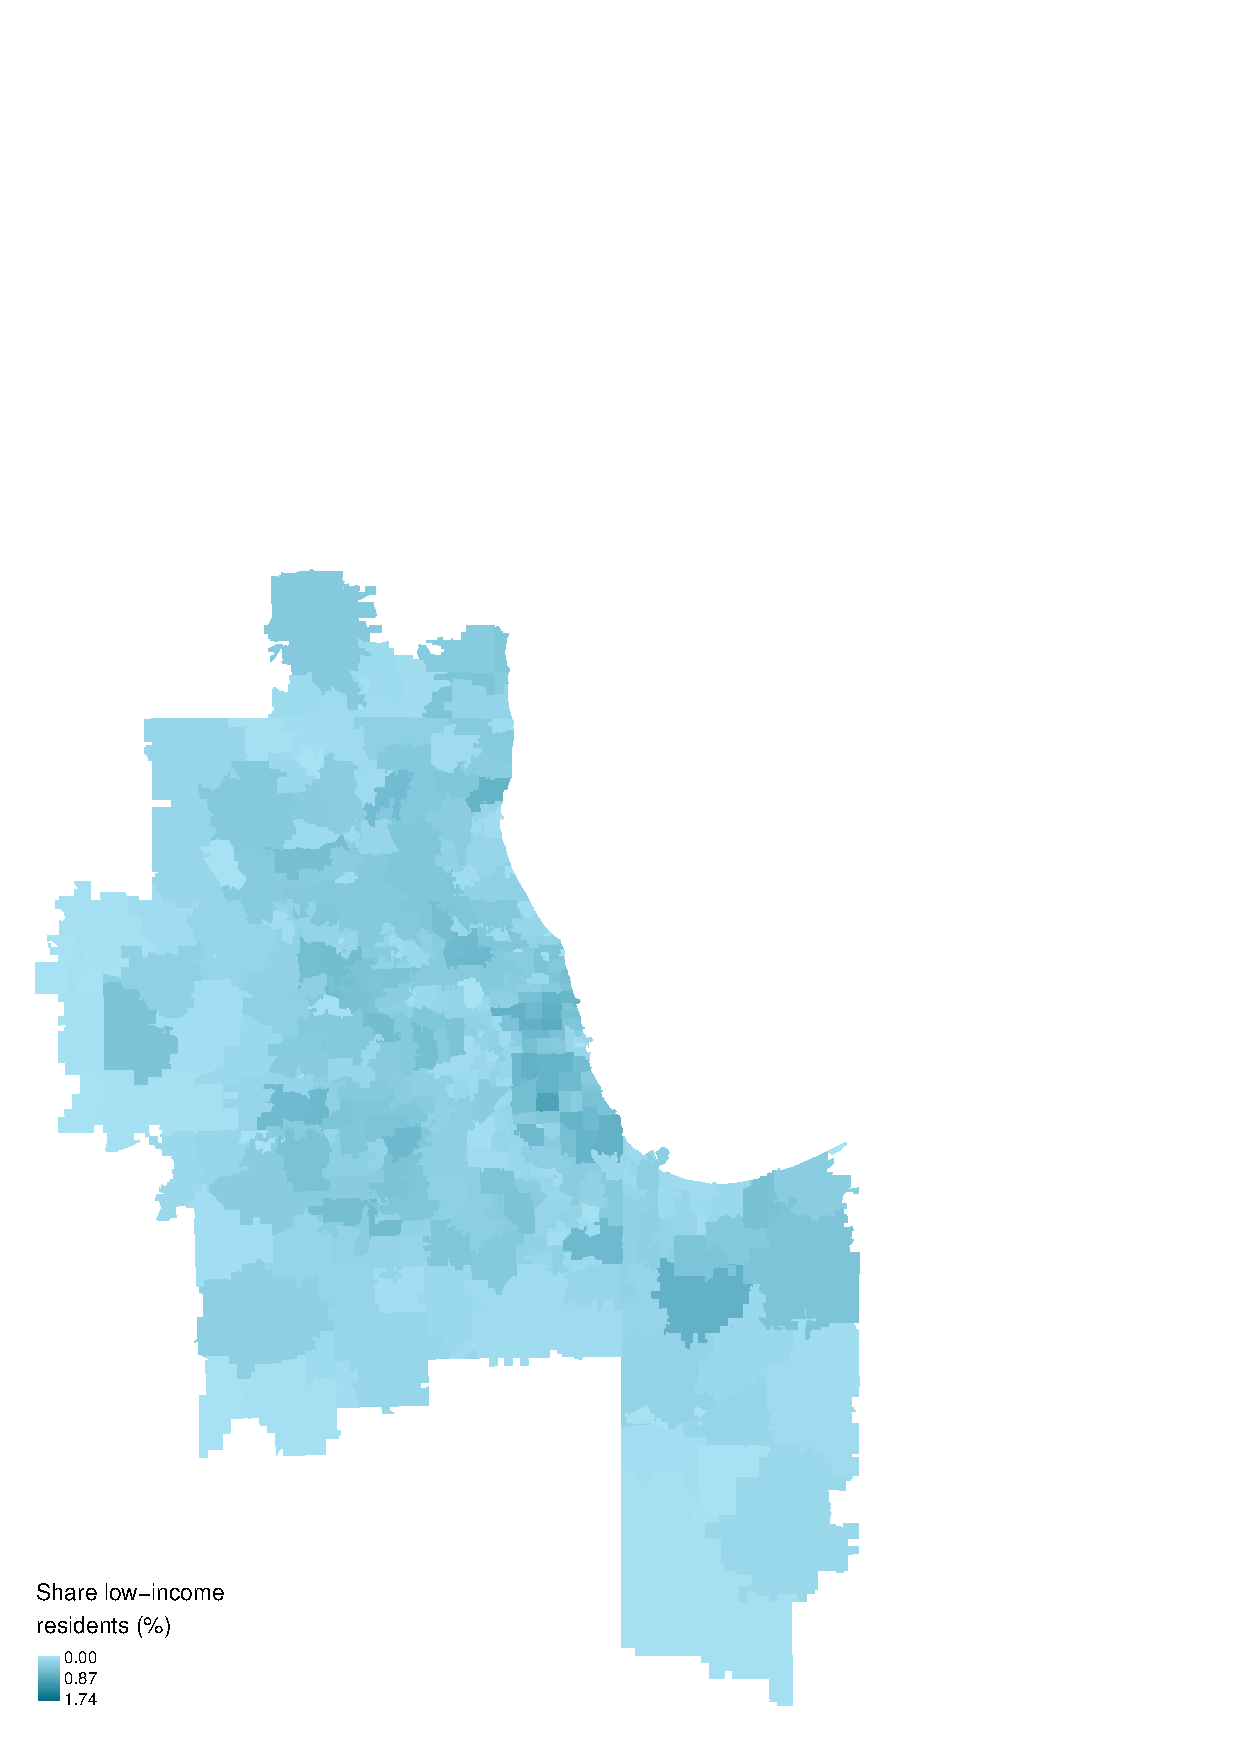
\includegraphics[width = 1\textwidth]
            {maps_shares/output/chicago2018_share_residents_lowinc}
    \end{subfigure}%
    \begin{subfigure}{.5\textwidth}
        \caption{Workers}
        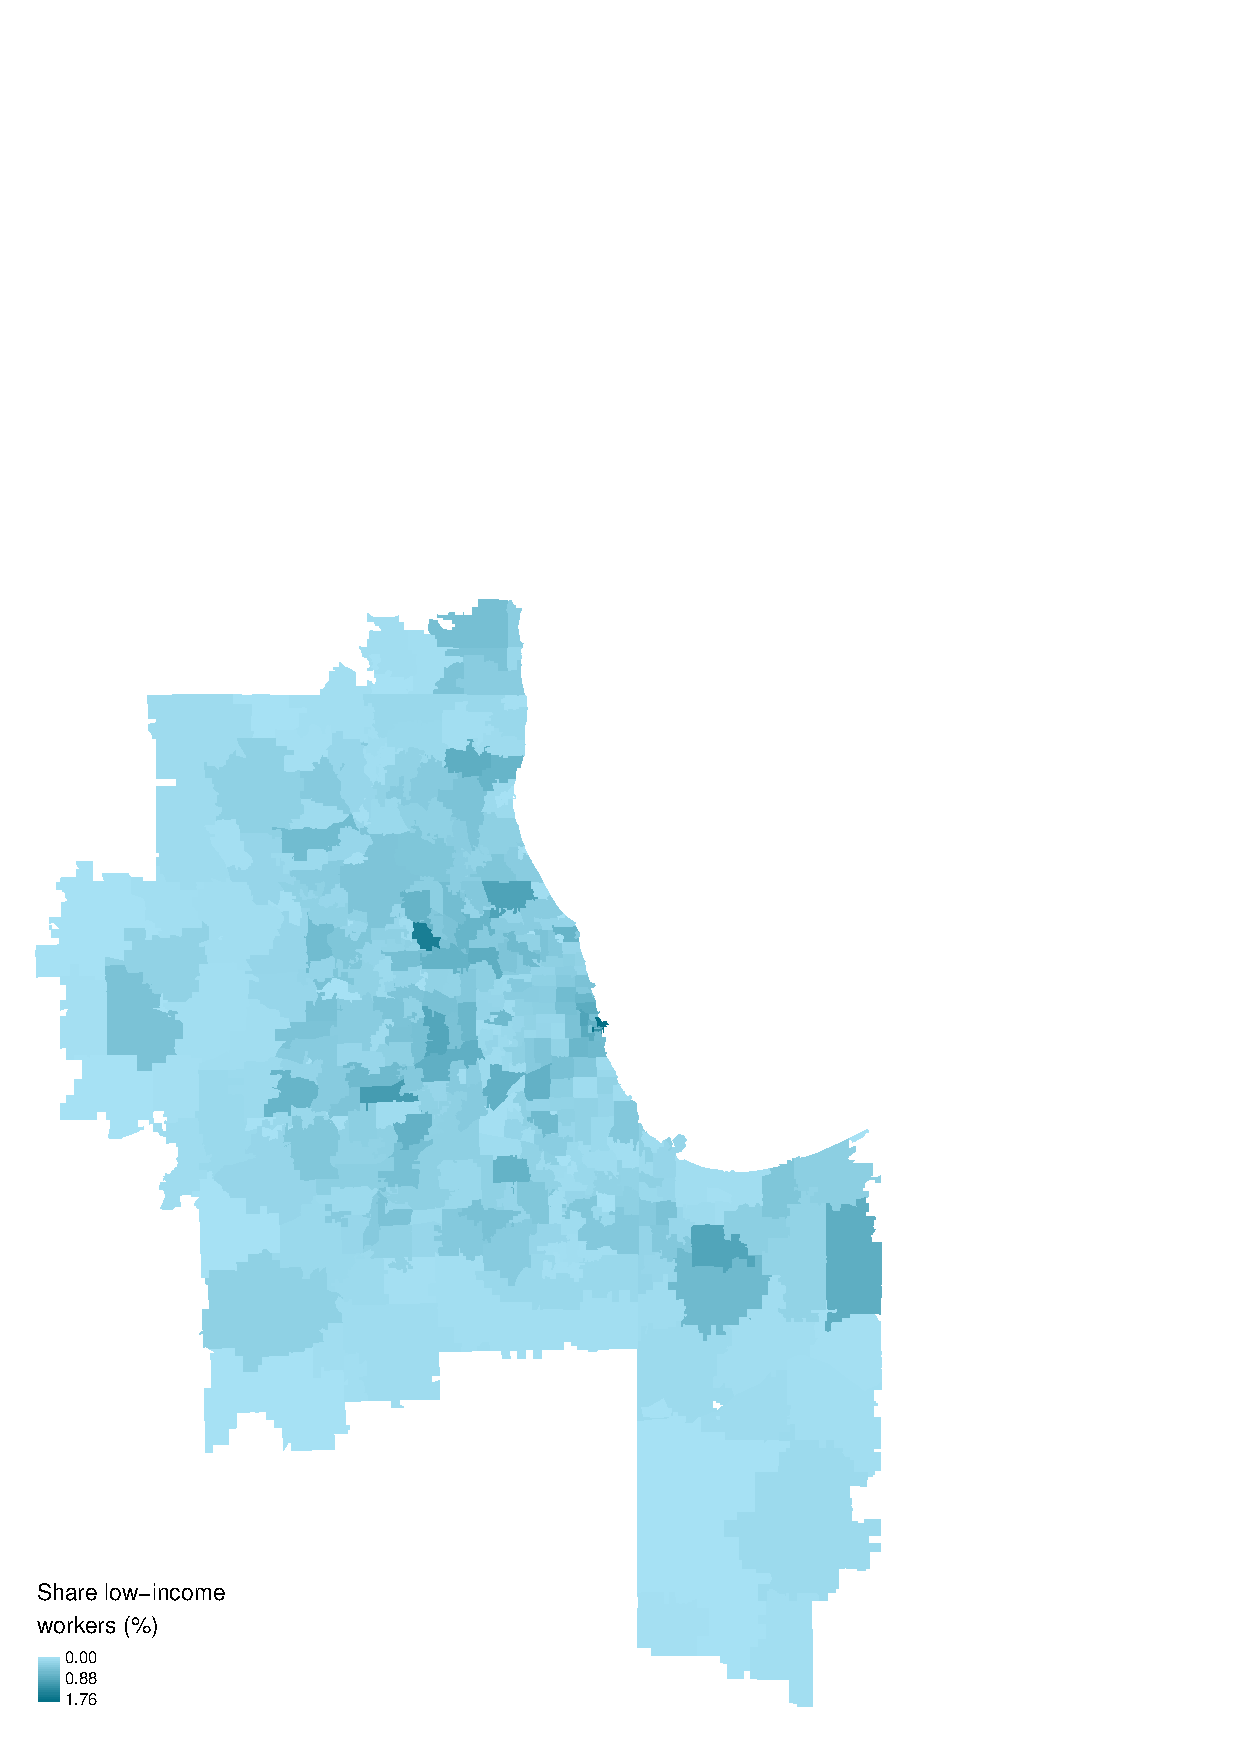
\includegraphics[width = 1\textwidth]
            {maps_shares/output/chicago2018_share_workers_lowinc}
    \end{subfigure}

    \begin{minipage}{.95\textwidth} \footnotesize
        \vspace{3mm}
        Notes:
        Data are from LODES \parencite{LODES} aggregated at the ZIP code level.
        The figure shows the share of low-income residents and workers out of
        the CBSA total in each ZIP code.
        Low-income workers are defined as those earning less than \$1,251 per
        month.
    \end{minipage}
\end{figure}

\clearpage
\begin{figure}[h!]
    \centering
    \caption{Distribution of statutory minimum wage changes}
    \label{fig:mw_changes_dist}

    \begin{subfigure}{.7\textwidth}
        \caption{Intensity}
        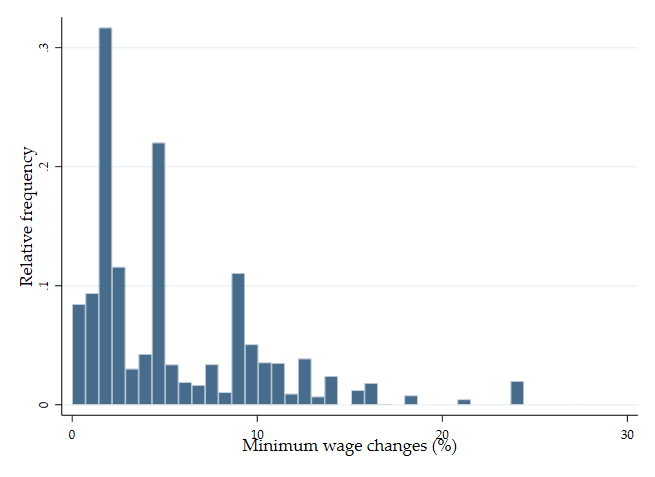
\includegraphics[width = \textwidth]
            {estimation_samples/output/pct_ch_mw_dist}
    \end{subfigure}\\
    \begin{subfigure}{.7\textwidth}
        \caption{Timing}
        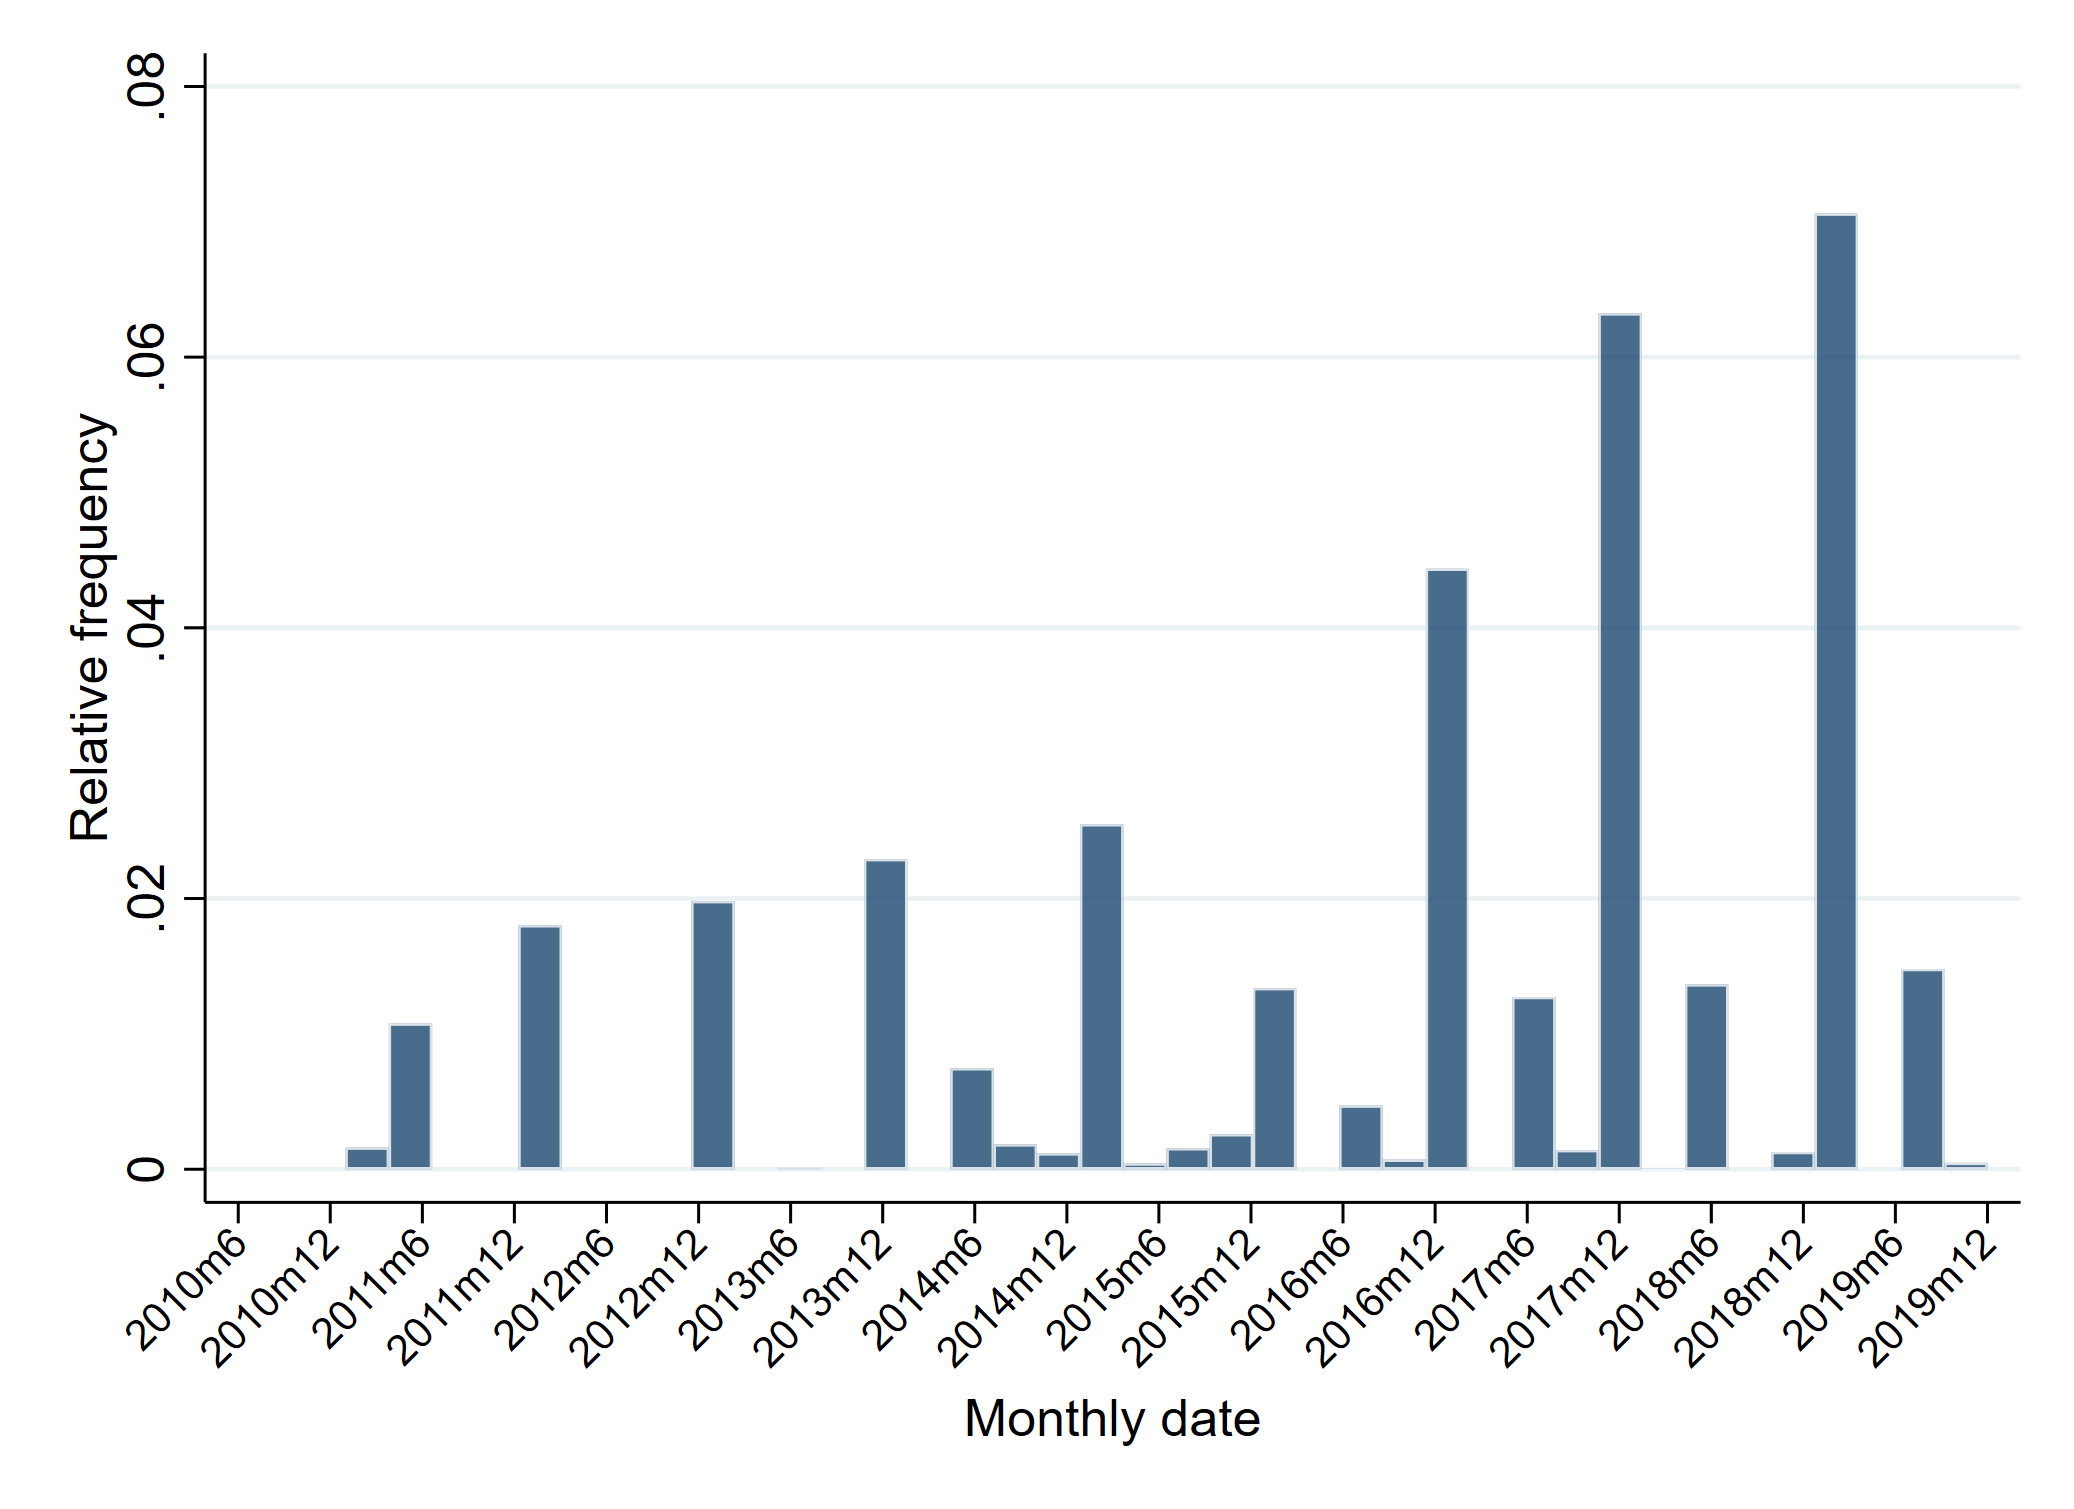
\includegraphics[width = \textwidth]
            {estimation_samples/output/pct_ch_mw_date_dist}
    \end{subfigure}

    \begin{minipage}{.95\textwidth} \footnotesize
        \vspace{3mm}
        Notes:
        Data are from the minimum wage panel described in 
        Section \ref{sec:mw_construction}.
        The histograms show the distribution of positive MW changes in the full 
        sample of ZIP codes available in the Zillow data.
        Panel (a) reports the intensity of the changes in percentage terms.
        Panel (b) plots the distribution of such changes over time.
    \end{minipage}
\end{figure}

\clearpage
\begin{figure}[h!]
    \centering
    \caption{Changes in minimum wage measures in the Chicago-Naperville-Elgin CBSA, July 2019}
    \label{fig:map_mw_chicago_jul2019}

    \begin{subfigure}{0.5\textwidth}
        \centering
        \caption*{Residence MW}
        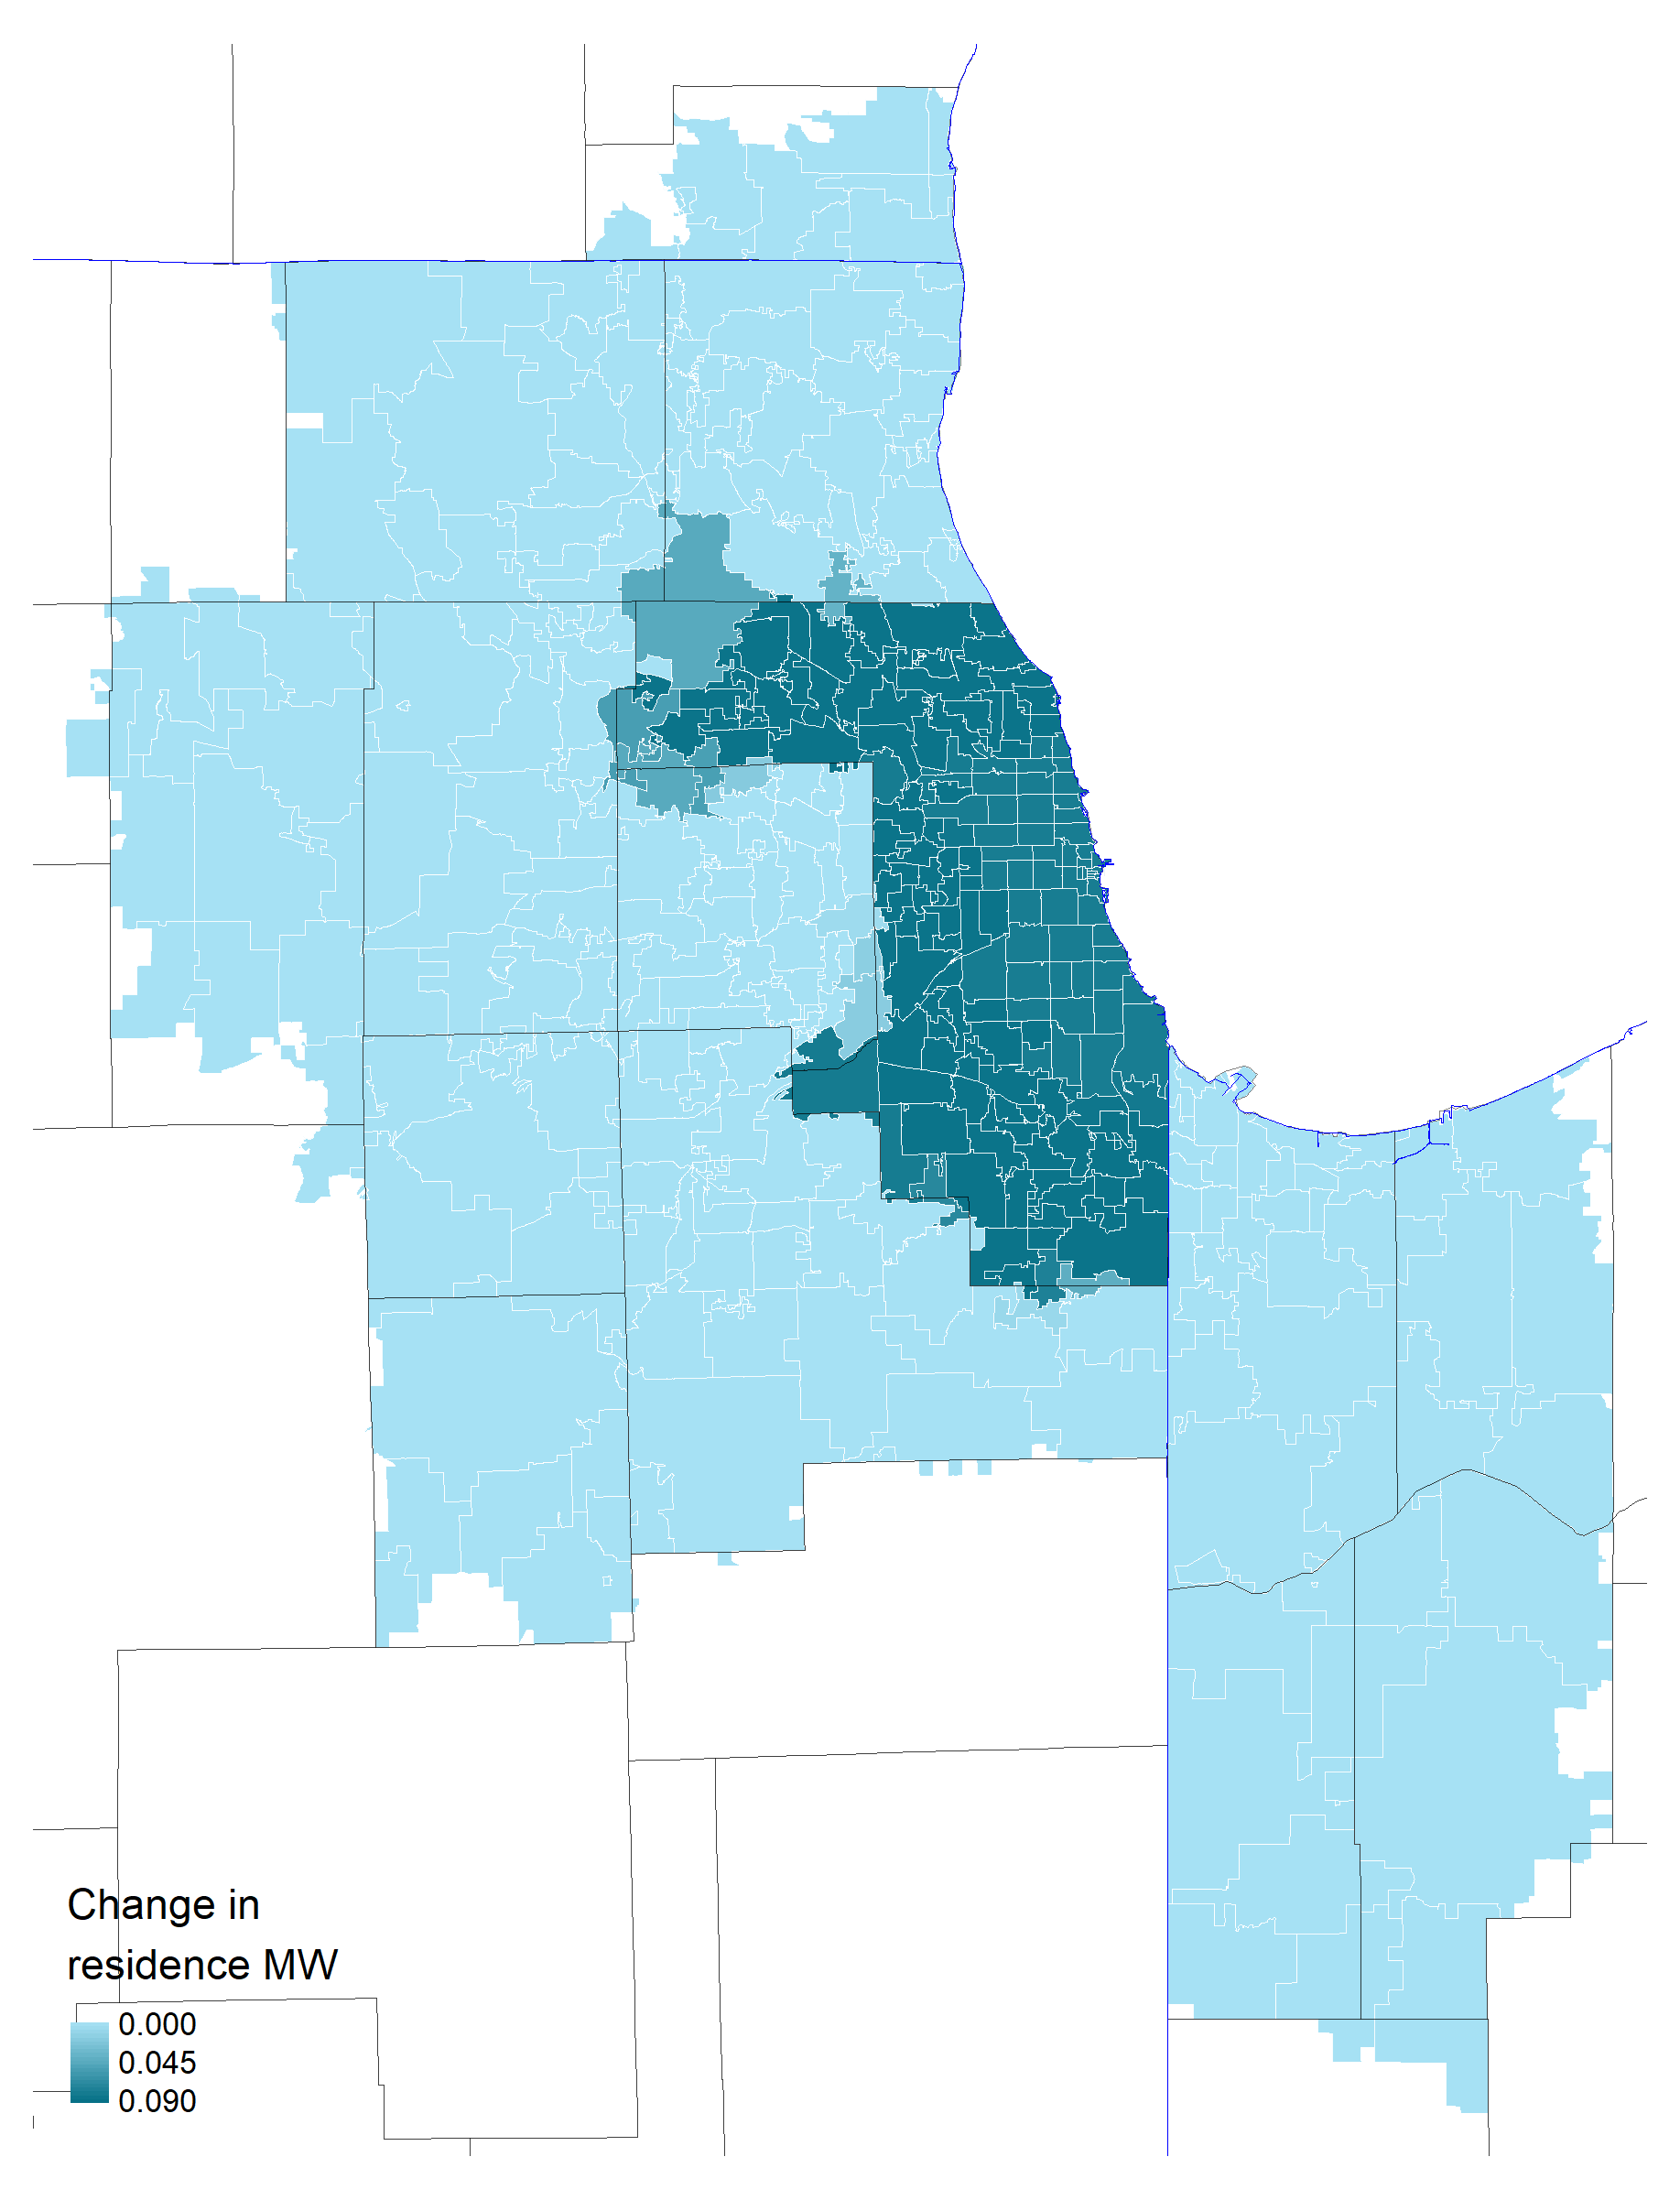
\includegraphics[width = 1\textwidth]
            {maps_events/output/chicago_2019-6_statutory_mw}
    \end{subfigure}%
    \begin{subfigure}{0.5\textwidth}
        \centering
        \caption*{Workplace MW}
        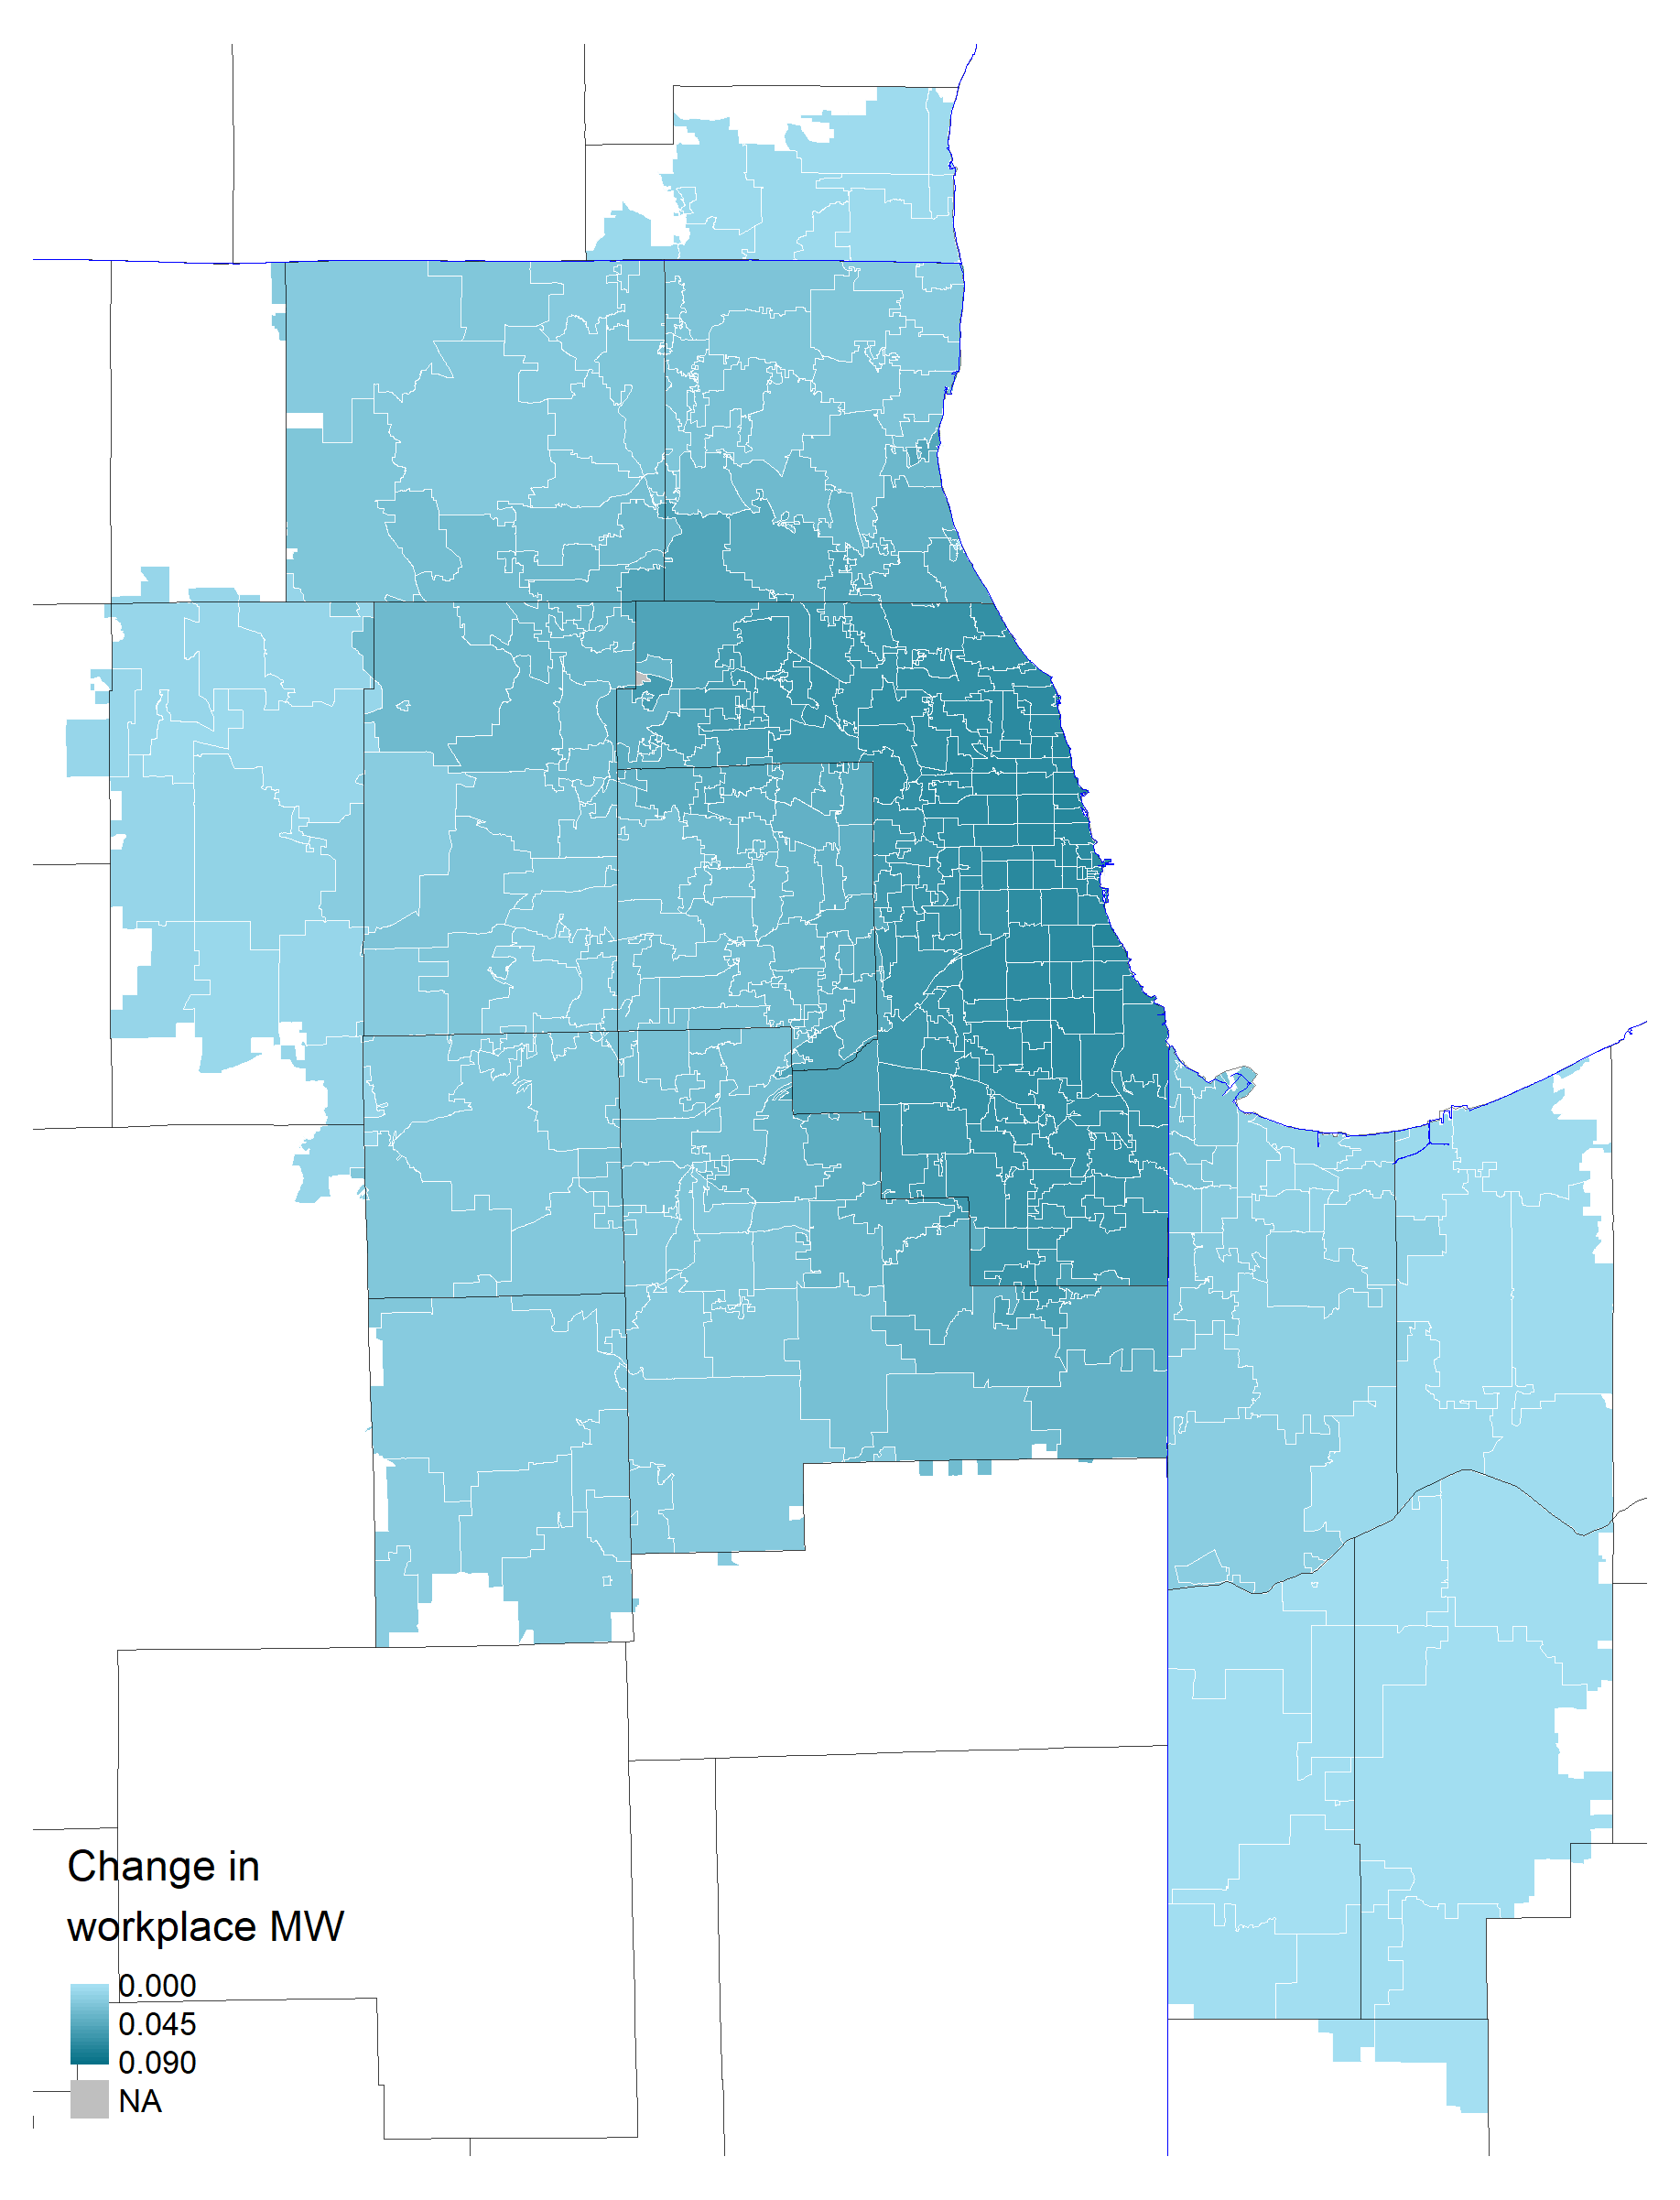
\includegraphics[width = 1\textwidth]
            {maps_events/output/chicago2019-6_wkp_mw}
    \end{subfigure}

    \begin{minipage}{.95\textwidth} \footnotesize
        \vspace{3mm}
        Notes: 
        Data are from the MW panel described in
        Section \ref{sec:data_mw_panel} and from LODES.
        The figures show changes in the MW measures in July 2019 in the 
        metropolitan area of Chicago.
        The figure on the left shows the change in the residence MW.
        The figure on the right shows the change in the workplace MW. 
        The residence MW is defined as the log of the statutory MW of the given
        ZIP code.
        The workplace MW is defined as the weighted average of the log of the
        statutory MW levels in workplace locations of a ZIP code's residents,
        where weights are given by commuting shares.
    \end{minipage}
\end{figure}

\clearpage

\begin{figure}[h!]
    \centering
    \caption{Estimates of the effect of the minimum wage on rents, baseline sample
             including leads and lags}
    \label{fig:dynamic_baseline}

    \begin{subfigure}{.65\textwidth}
        \caption{Leads and lags of the workplace MW}
        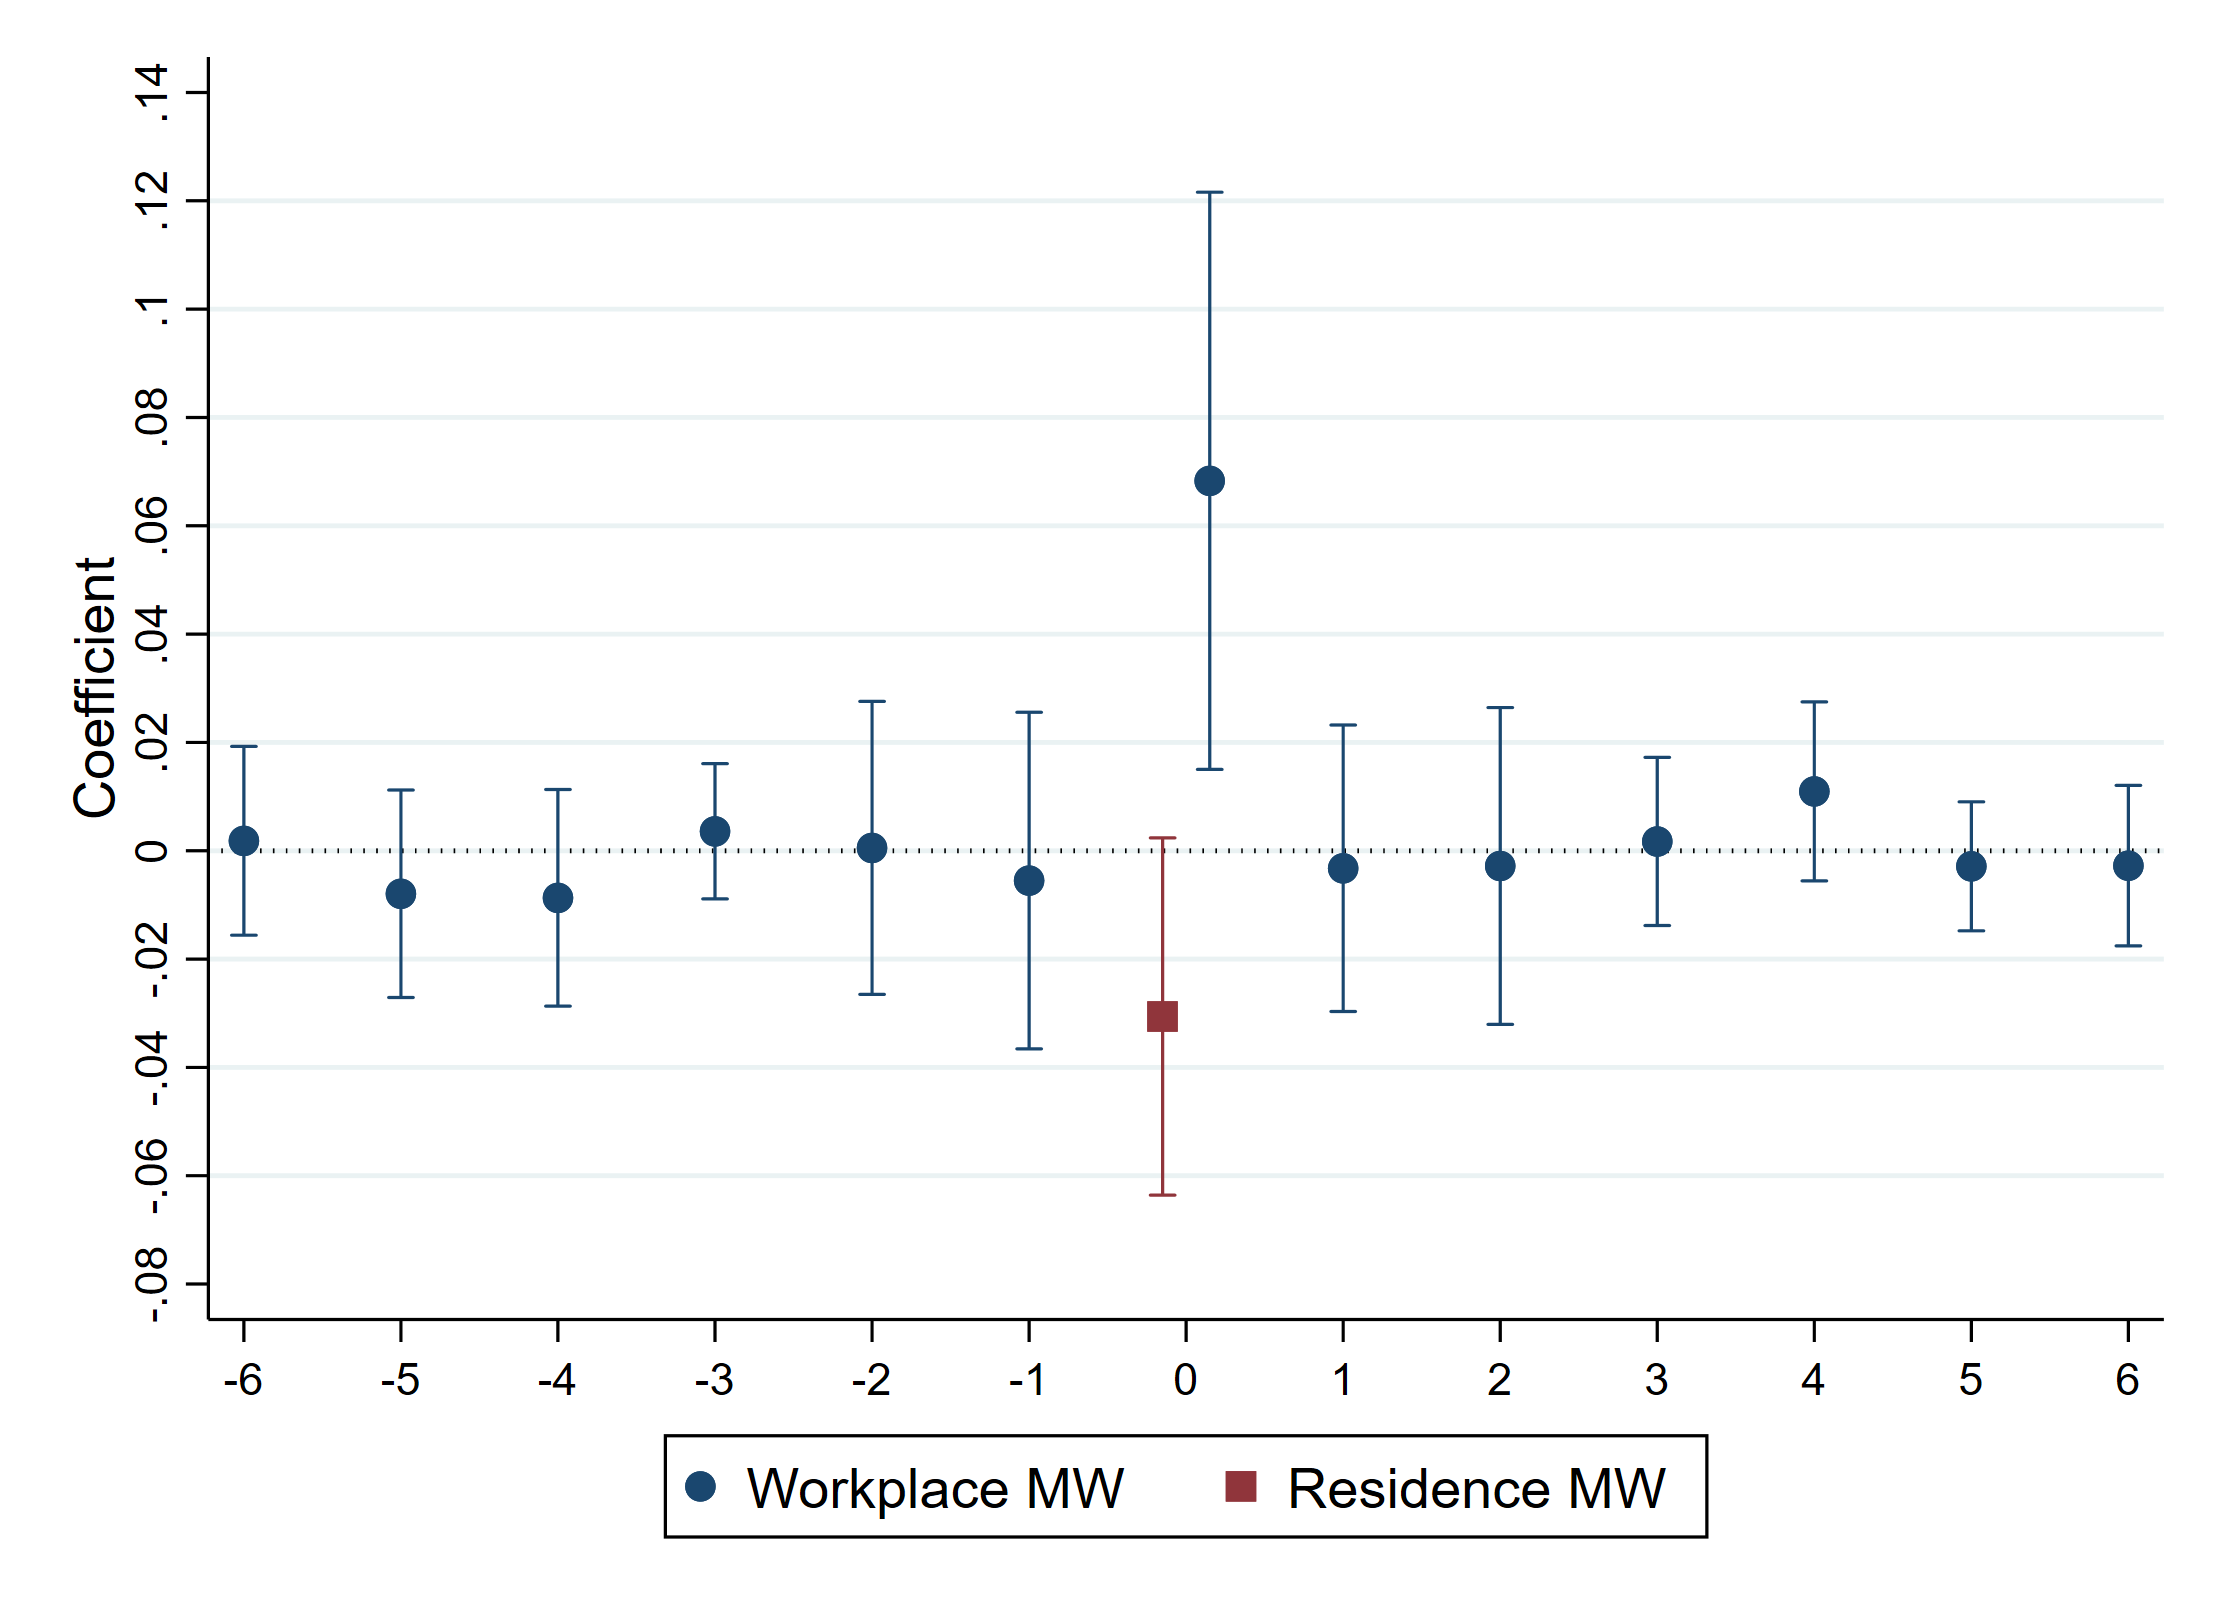
\includegraphics[width = 1\textwidth]
            {fd_baseline/output/fd_both_mw_wkp_only_dynamic}
    \end{subfigure}\\
    \begin{subfigure}{.65\textwidth}
        \caption{Leads and lags of the residence MW}
        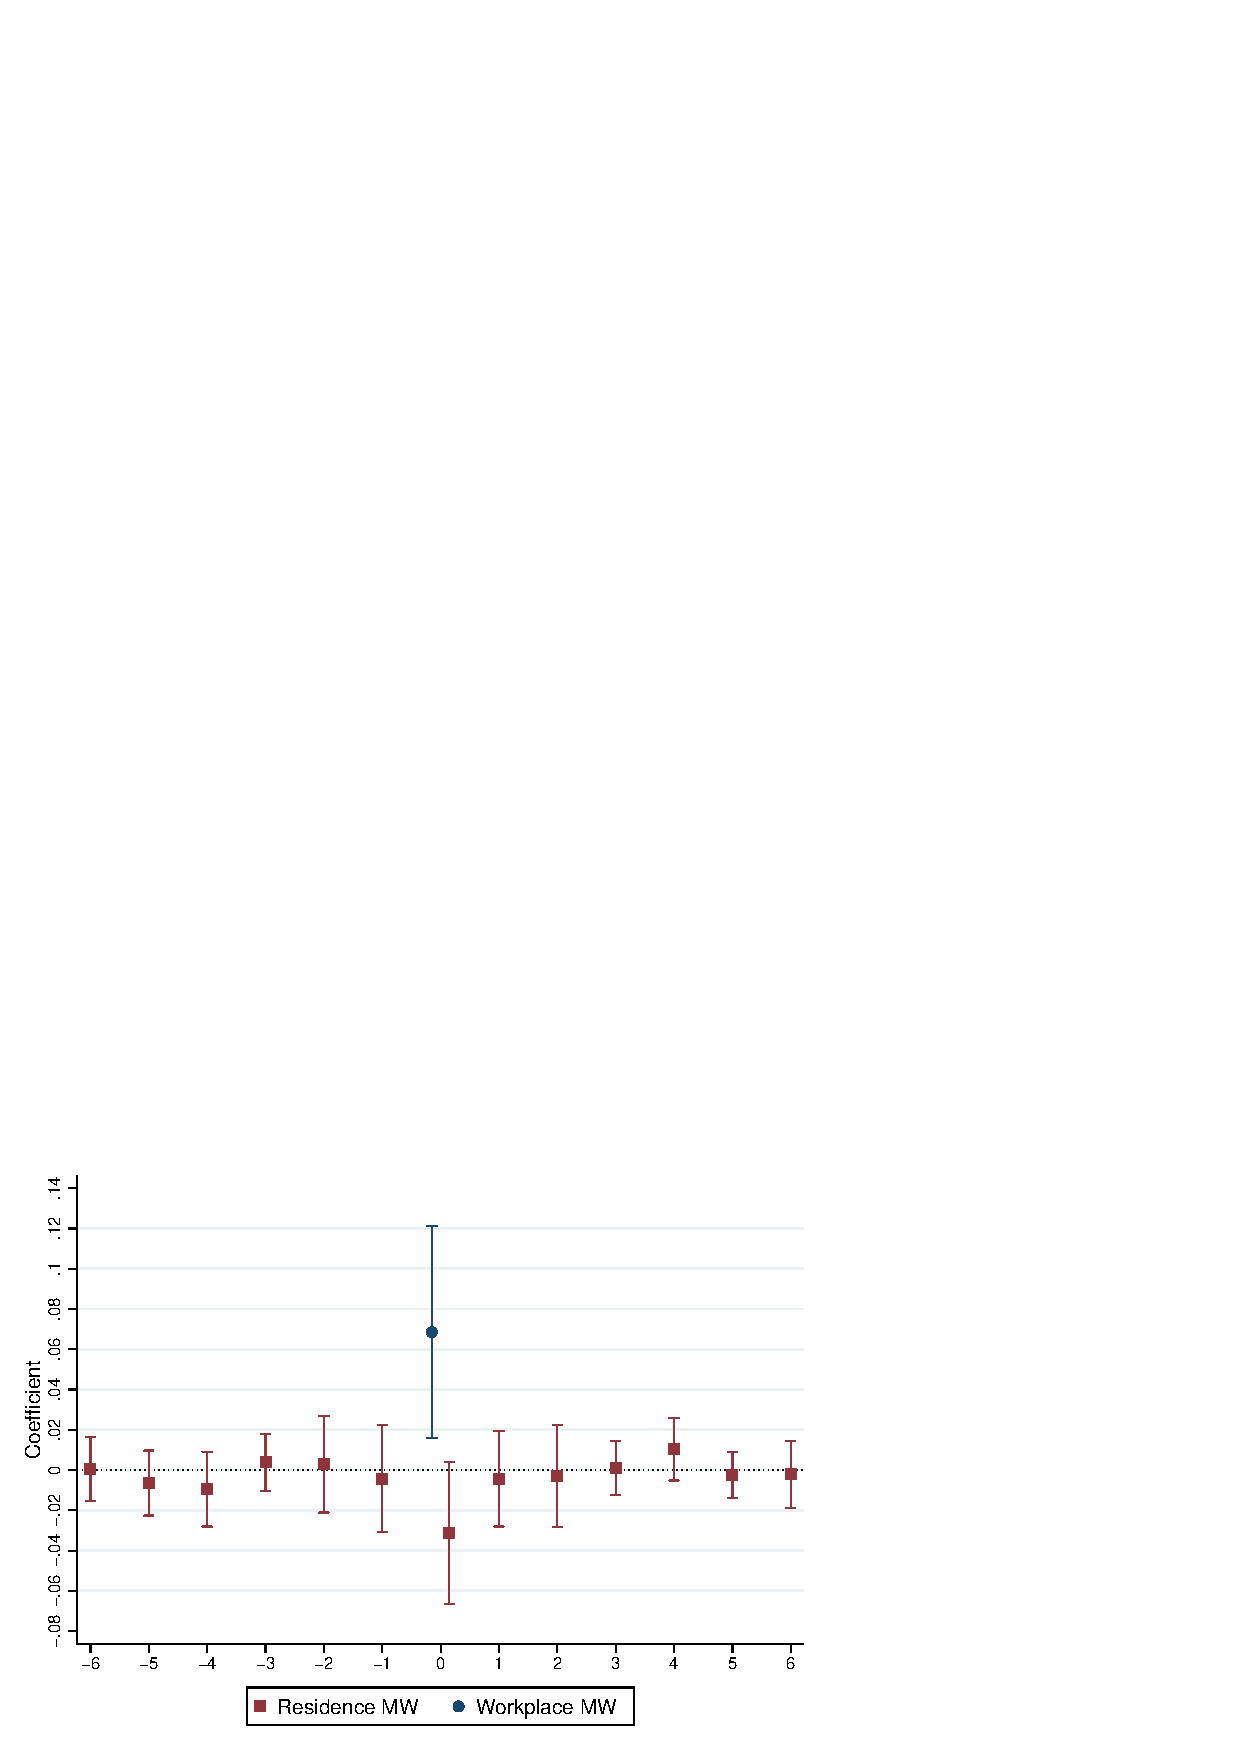
\includegraphics[width = 1\textwidth]
            {fd_baseline/output/fd_both_mw_res_only_dynamic}
    \end{subfigure}

    \begin{minipage}{.95\textwidth} \footnotesize
        \vspace{3mm}
        Notes:
        Data are from the baseline estimation sample described in Section 
        \ref{sec:data_final_panel}.
        All panels plot coefficients from regressions of the log of rents per
        square foot on the residence and workplace MW measures, varying the 
        number of leads and lags of each MW variable included.
        Panel (a) includes six leads and lags of the workplace MW measure.
        Panel (b) includes six leads and lags of the residence MW measure.
        All regressions are estimated in first differences and include 
        time-period fixed effects and economic controls that vary at the 
        county by month and county by quarter levels.
        The measure of rents per square foot correspond to the Single Family, 
        Condominium and Cooperative houses from Zillow described in Section
        \ref{sec:data_rents}.
        The residence MW is defined as the log statutory MW in the same ZIP code.
        The workplace MW is defined as the log statutory MW where the average 
        resident of the ZIP code works, constructed using LODES 
        origin-destination data described in Section \ref{sec:data_mw_measures}.
        Economic controls from the QCEW (Section \ref{sec:data_other}) include the
        change of the following variables: the log of the average wage, the log
        of employment, and the log of the establishment count for the sectors 
        ``Information,'' ``Financial activities,'' and ``Professional and 
        business services.''
        95\% pointwise confidence intervals are obtained from standard errors 
        clustered at the state level.
    \end{minipage}
\end{figure}

\clearpage
\begin{figure}[h!]
    \centering
    \caption{Distributions of estimated shares pocketed by landlords under a 
            counterfactual federal MW policy of \$9, urban ZIP codes}
    \label{fig:cf_hist_rents_wages_shares}

    \begin{subfigure}{0.65\textwidth}
        \caption*{Share of additional income pocketed by landlords}
        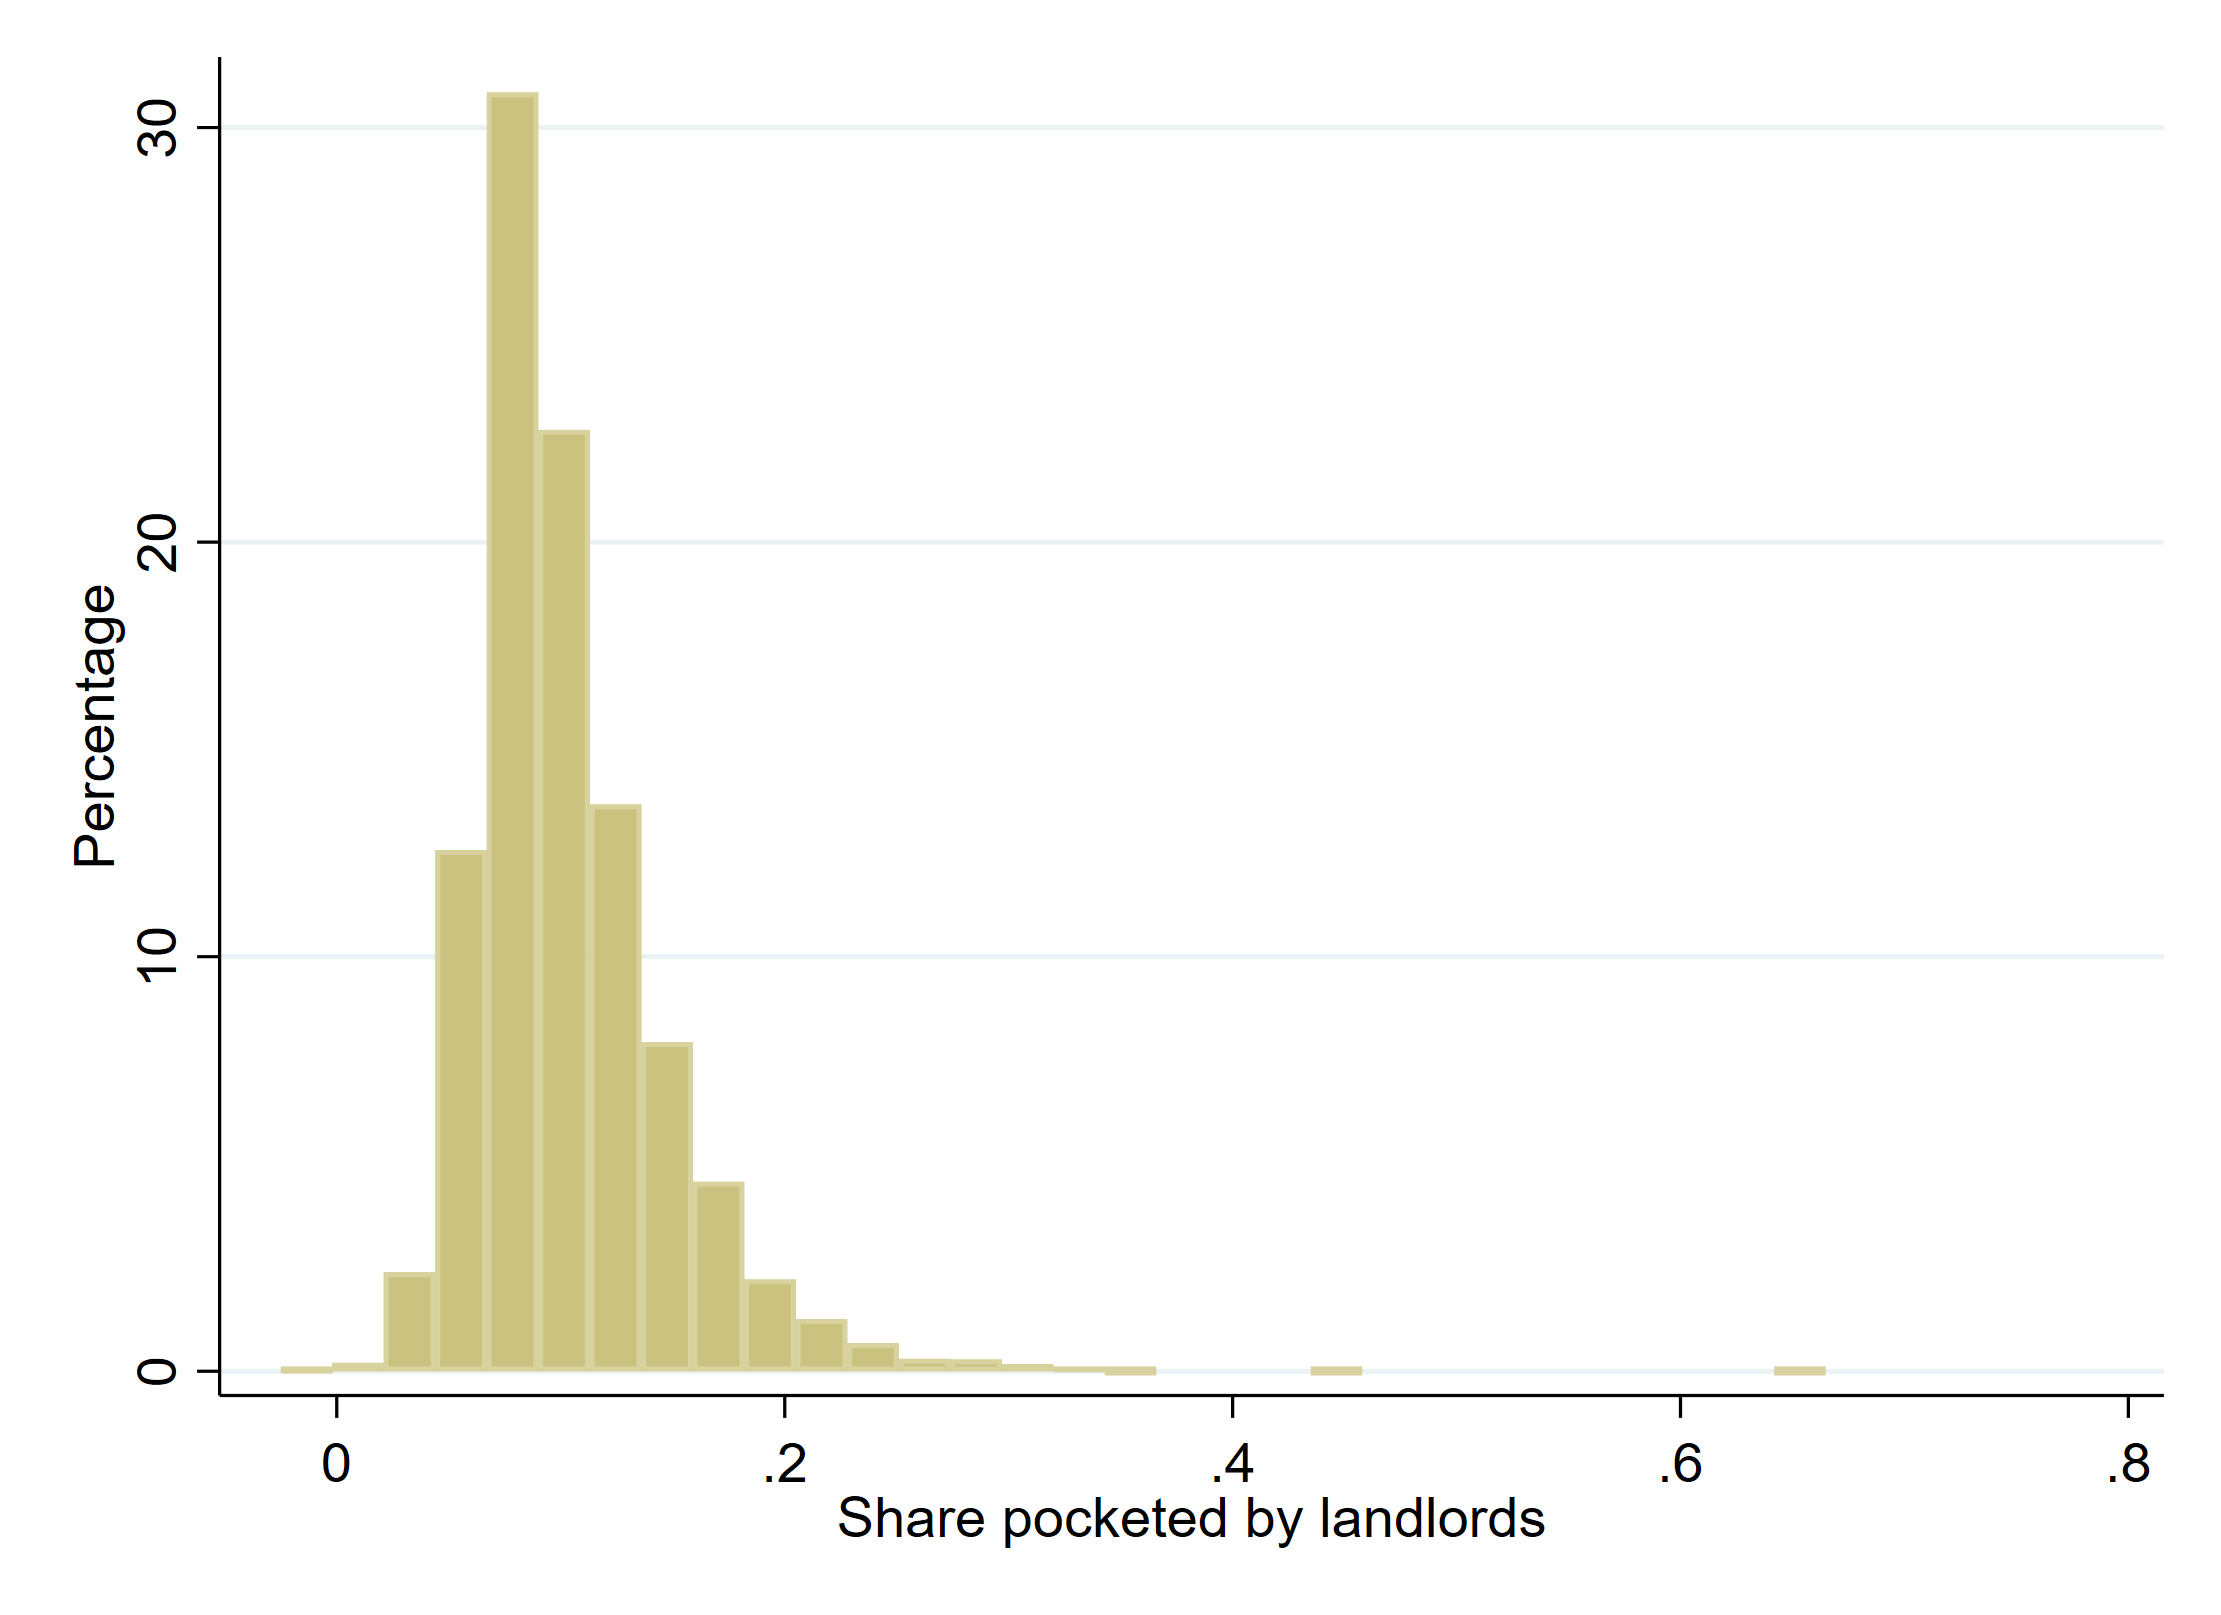
\includegraphics[width = 1\textwidth]{counterfactuals/output/hist_rho.png}
    \end{subfigure}\\
    \begin{subfigure}{0.5\textwidth}
        \caption*{Change in log rents}
        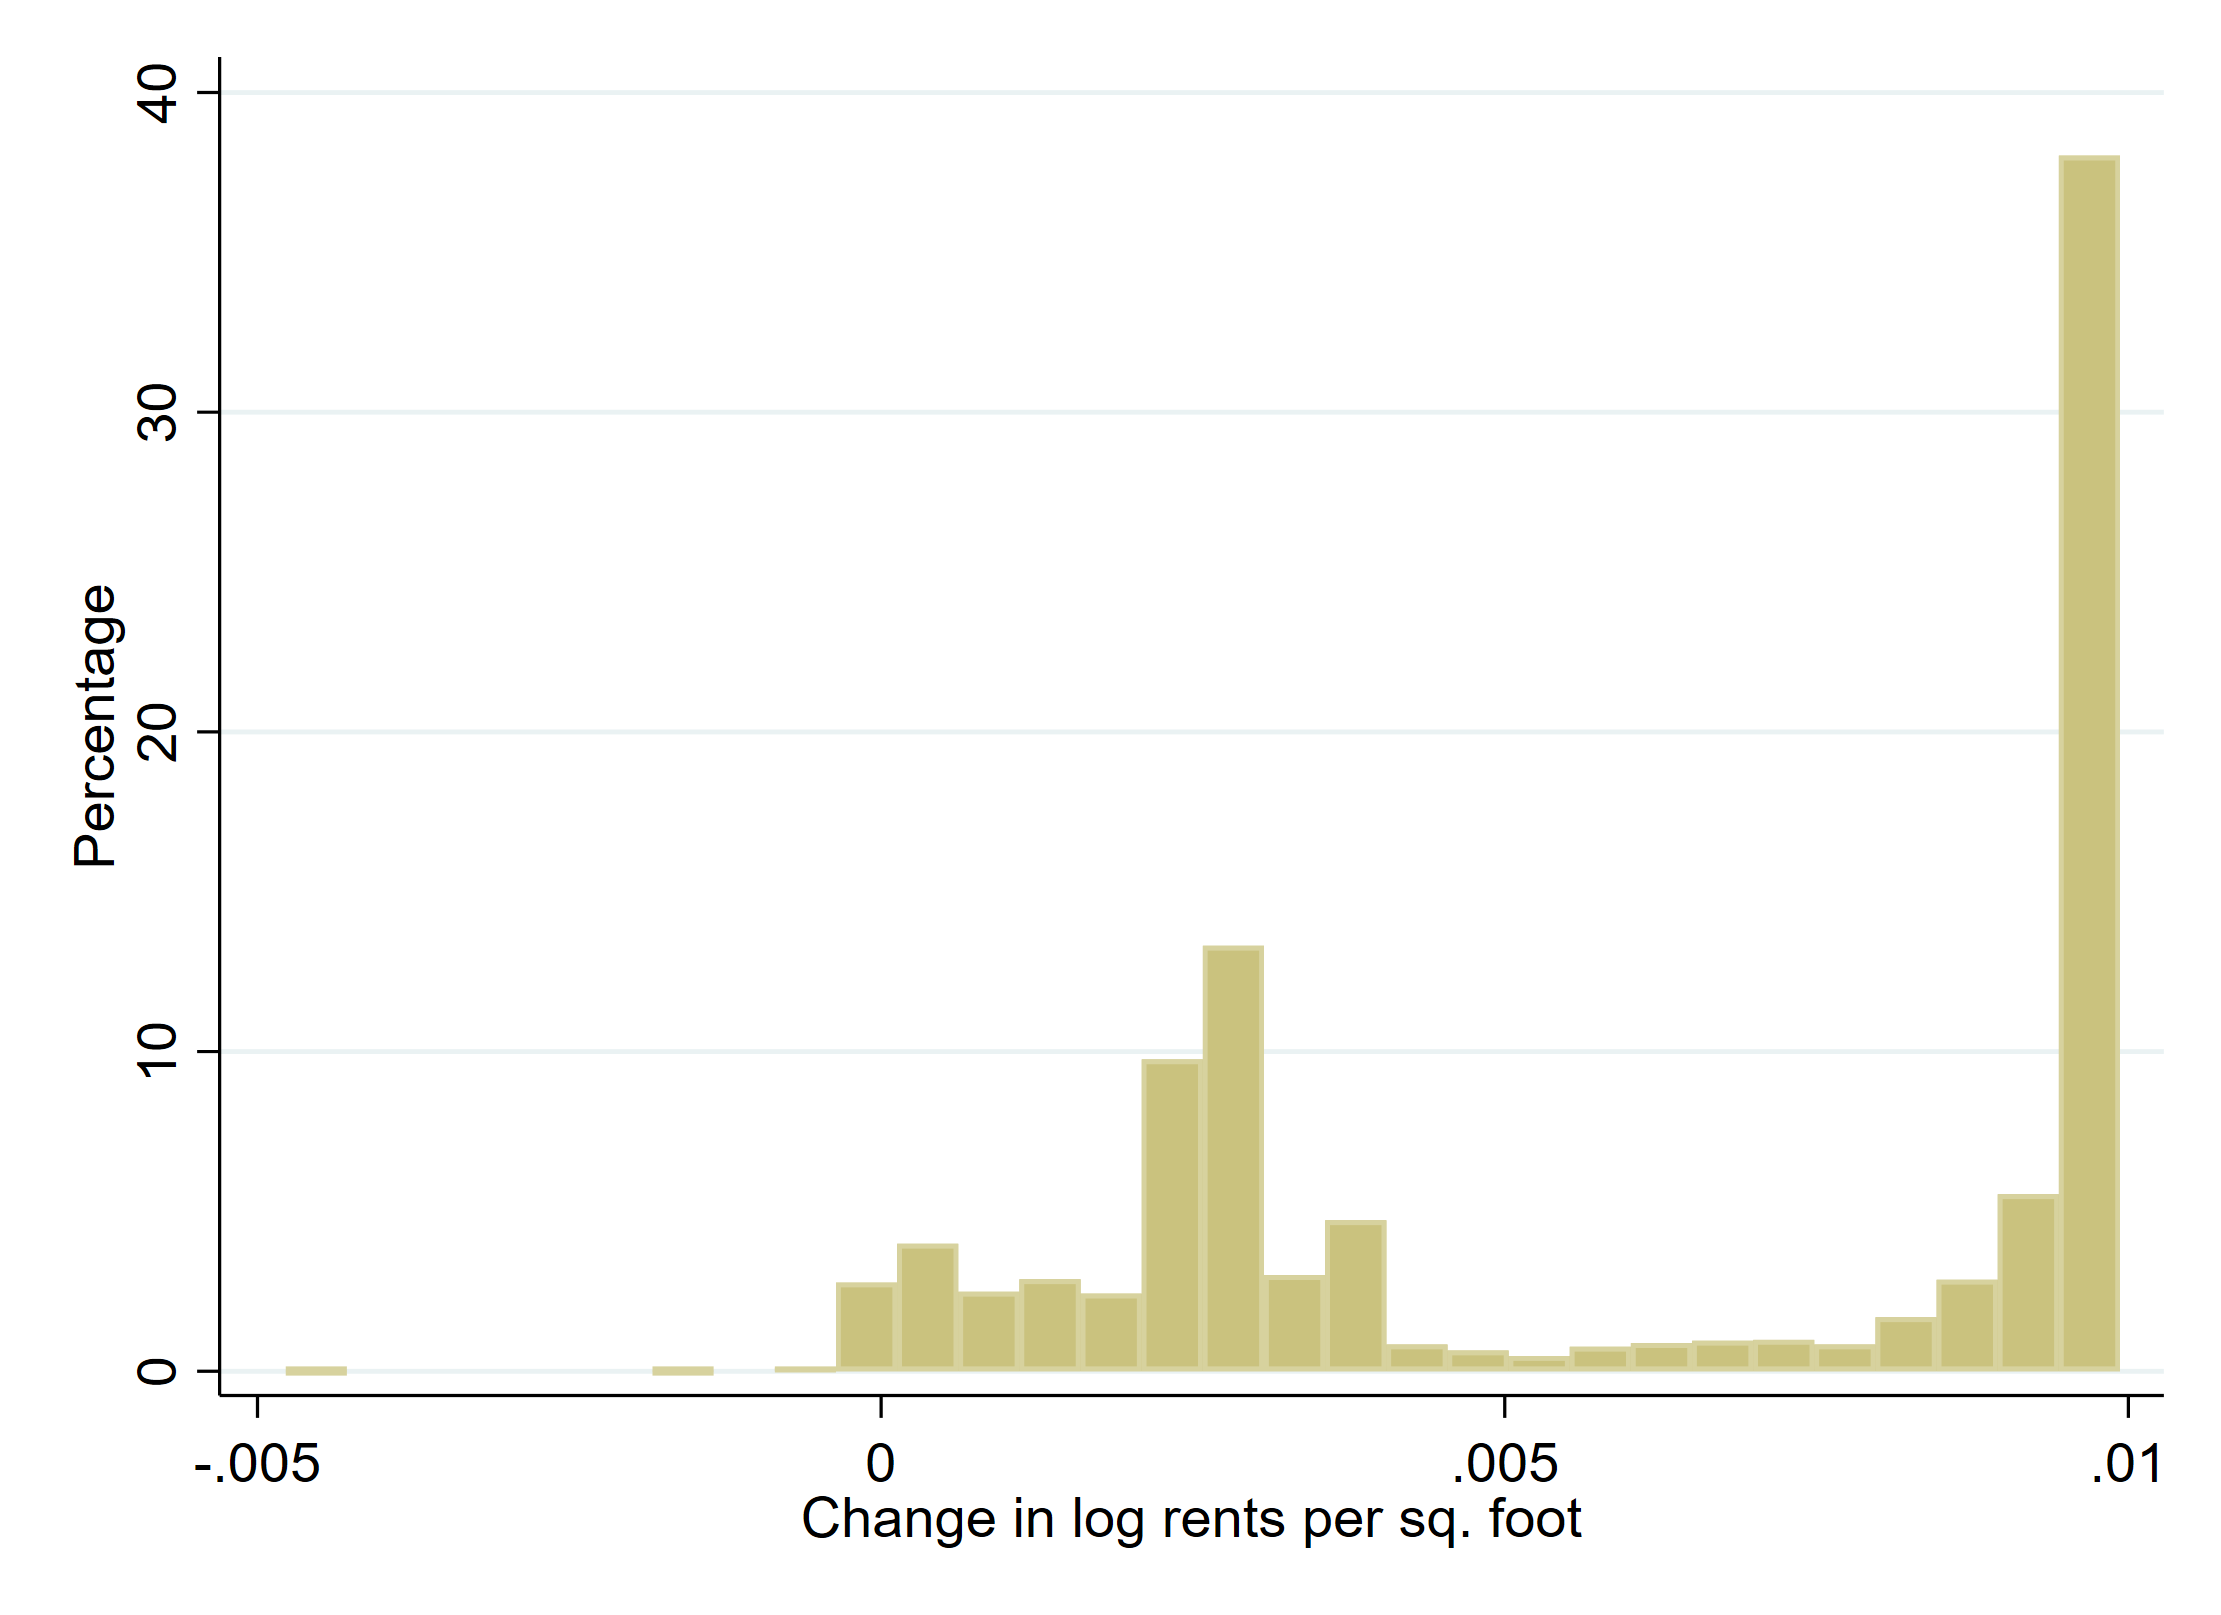
\includegraphics[width = .95\textwidth]{counterfactuals/output/hist_change_ln_rents.png}
    \end{subfigure}%
    \begin{subfigure}{0.5\textwidth}
        \caption*{Change in log total wages}
        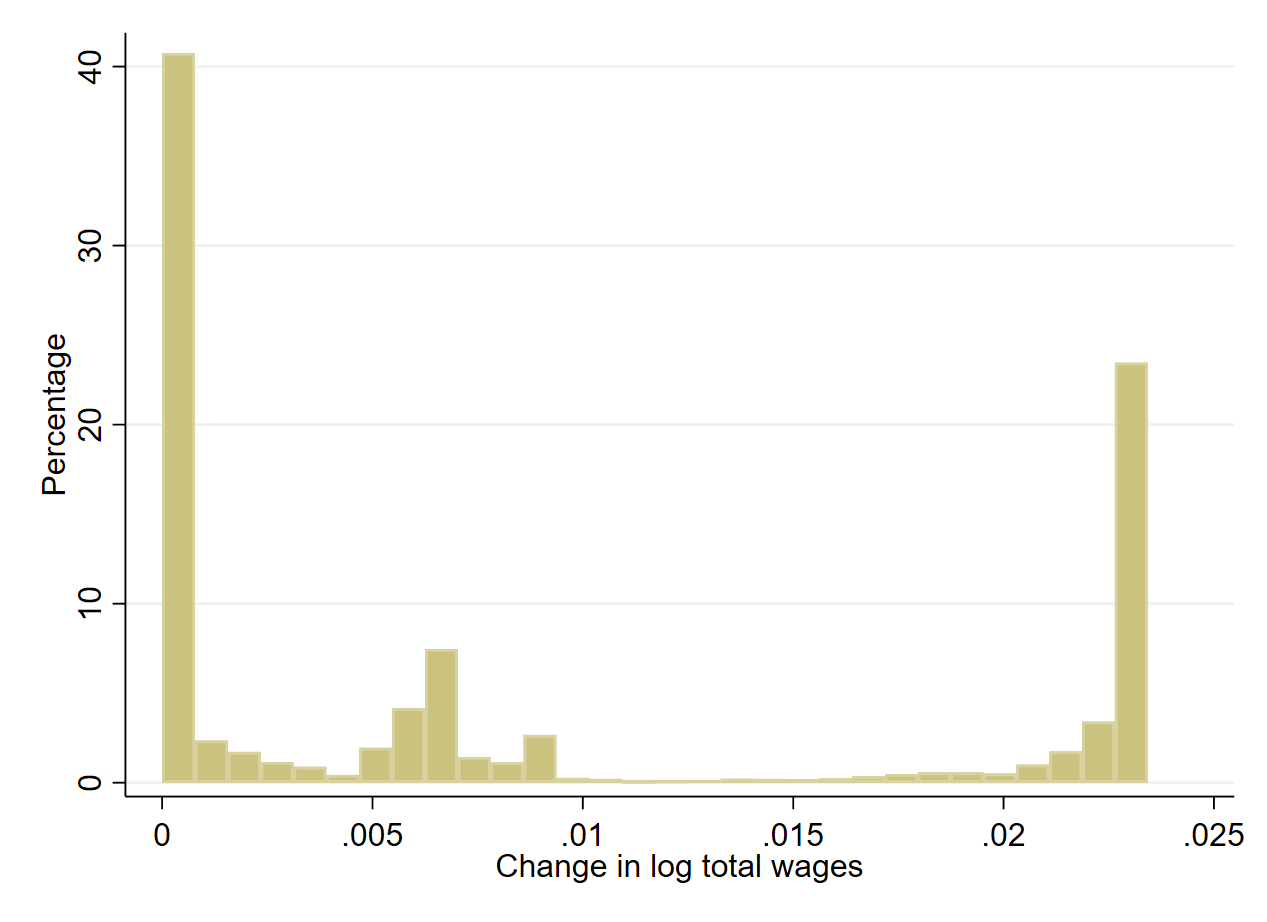
\includegraphics[width = .95\textwidth]{counterfactuals/output/hist_change_ln_wagebill.png}
    \end{subfigure}

    \begin{minipage}{.95\textwidth} \footnotesize
        \vspace{3mm}
        Notes:
        Data are from the MW panel and from LODES, described in
        Section \ref{sec:data_mw_panel}.
        The top figure shows the distribution of the estimated ZIP code-specific
        shares of the additional income pocketed by landlords (``share pocketed''), 
        the bottom left figure shows estimated changes in log rents, and 
        the bottom right figure shows estimated changes in log total wages.
        The computations are based on a counterfactual increase to \$9 in the 
        federal MW in January 2020, holding constant other MW policies in their 
        December 2019 levels.
        The unit of observation is the urban ZIP code, where we define a ZIP code 
        as urban if it belongs to a CBSA with at least 80\% of its population 
        classified as urban by the 2010 Census.
        The share pocketed is defined as the ratio between the percent increase 
        in rents and the percent increase in total wages multiplied by the share 
        of housing expenditure in the ZIP code.
        To estimate it we follow the procedure described in Section 
        \ref{sec:counterfactual}, assuming the following parameter values: 
        $\beta = 0.0546$, $\gamma = -0.0207$, $\varepsilon = 0.1083$, and 
        $s = 0.35$.
    \end{minipage}
\end{figure}

\clearpage
\begin{figure}[h!]
    \centering
    \caption{Estimated landlord shares and counterfactual increases in log rents
            and log total wages, ZIP codes in the Chicago-Naperville-Elgin CBSA}
    \label{fig:map_chicago_cf_rents_wages_shares}

    \begin{subfigure}{.5\textwidth}
        \caption*{Landlord share}
        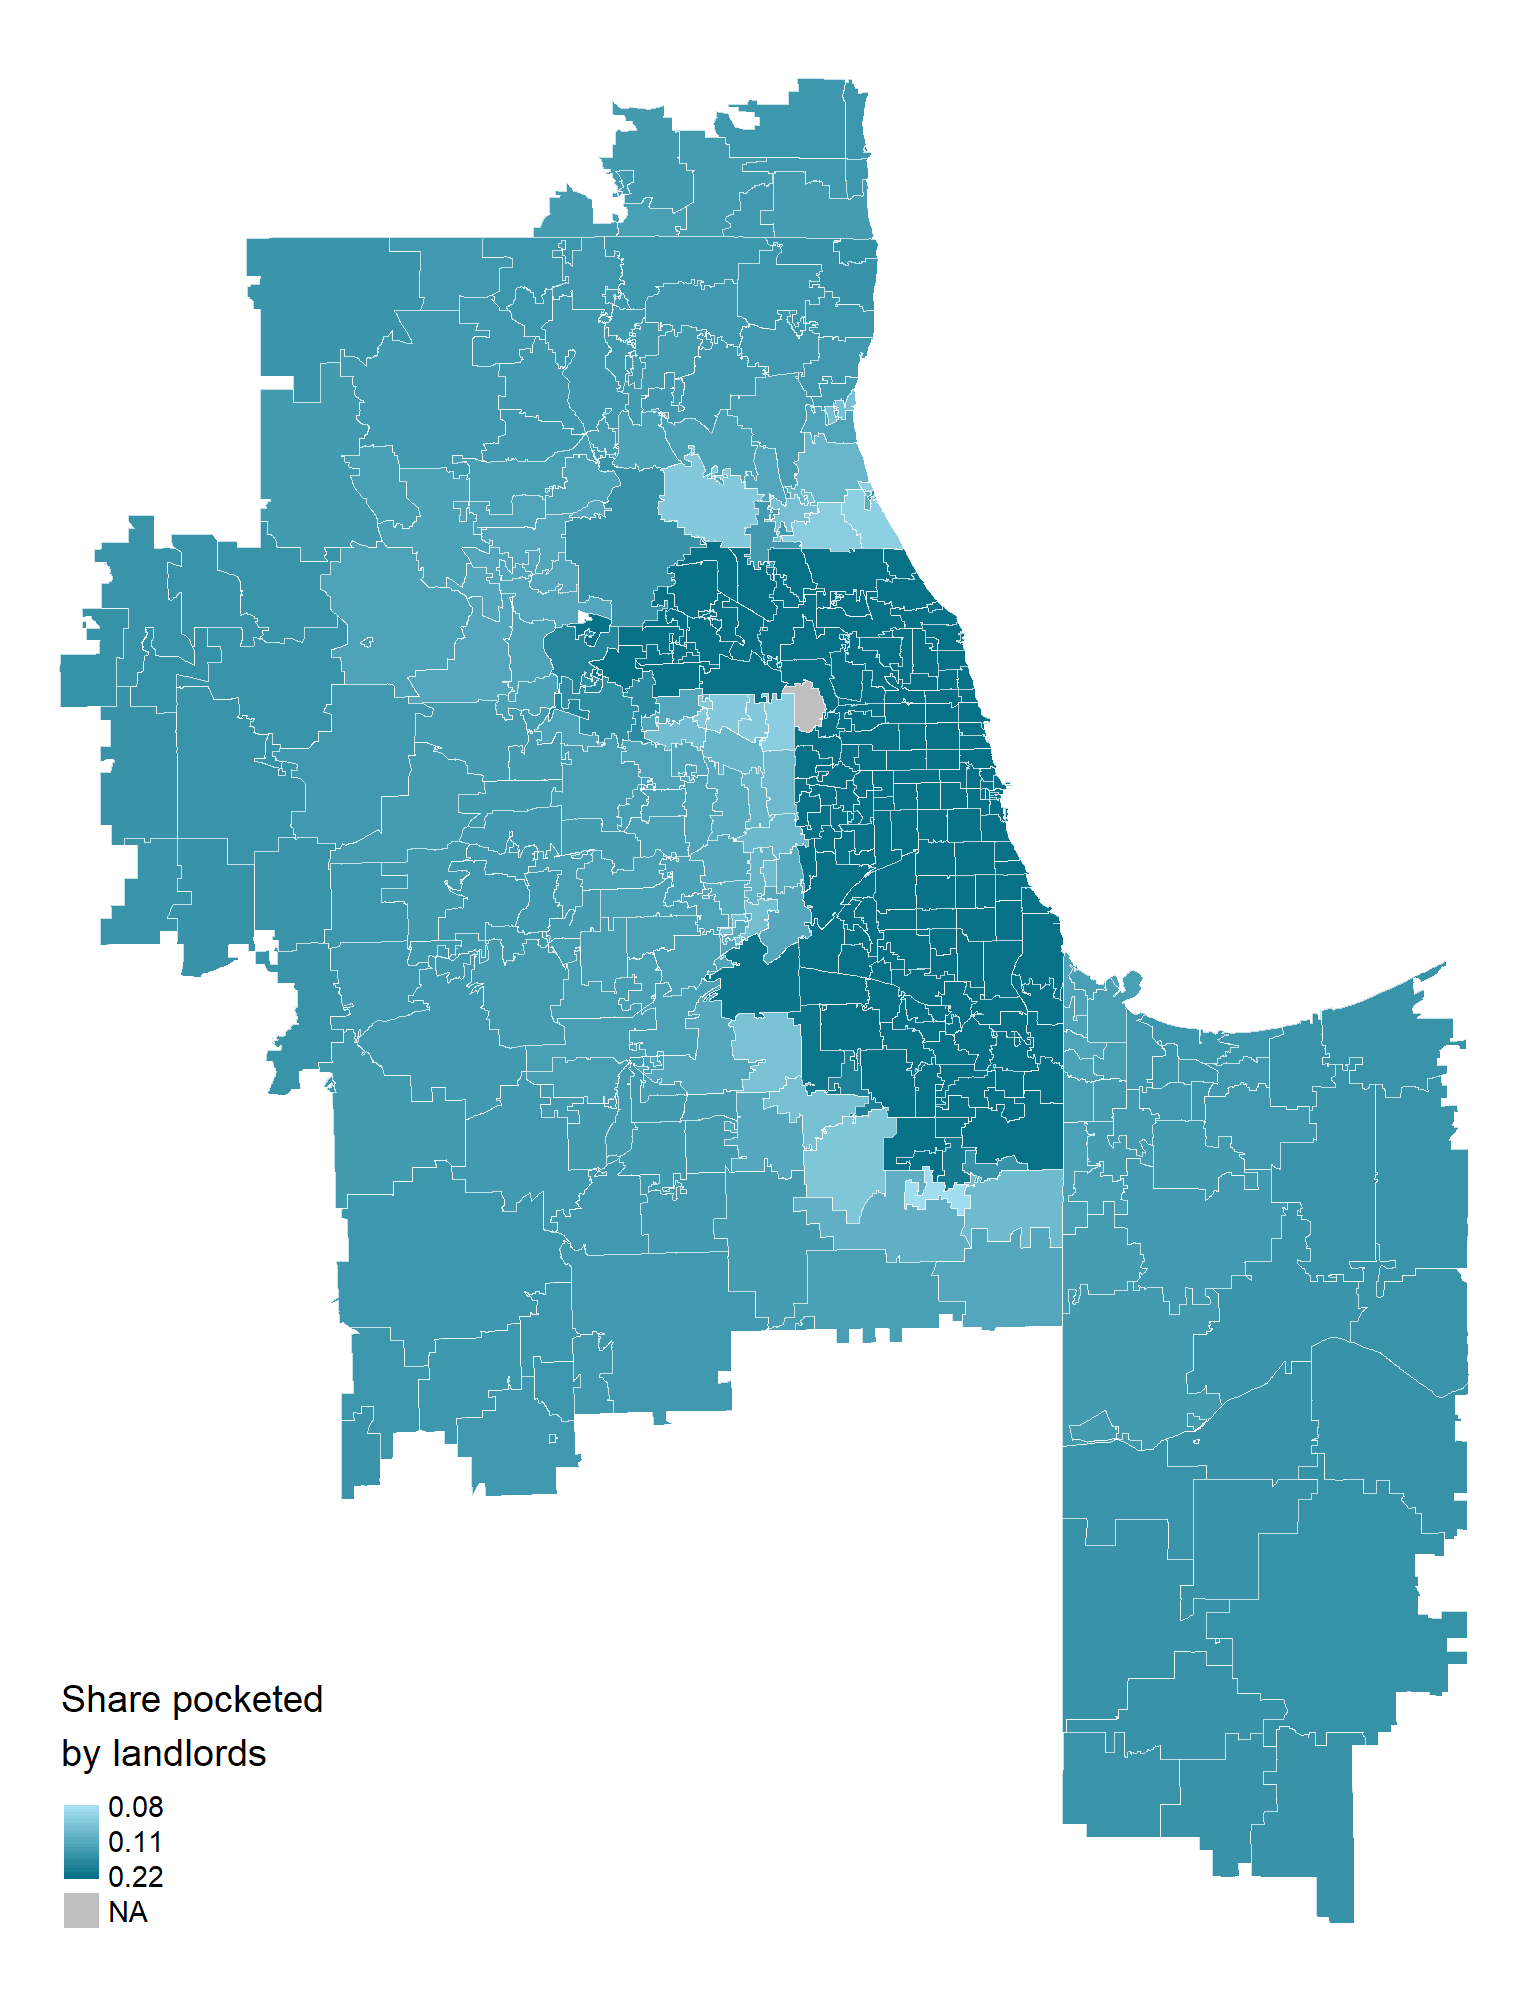
\includegraphics[width = 1\textwidth]
            {counterfactuals/output/chicago_rho.png}
    \end{subfigure}\\
    \begin{subfigure}{.35\textwidth}
        \caption*{Changes in log rents}
        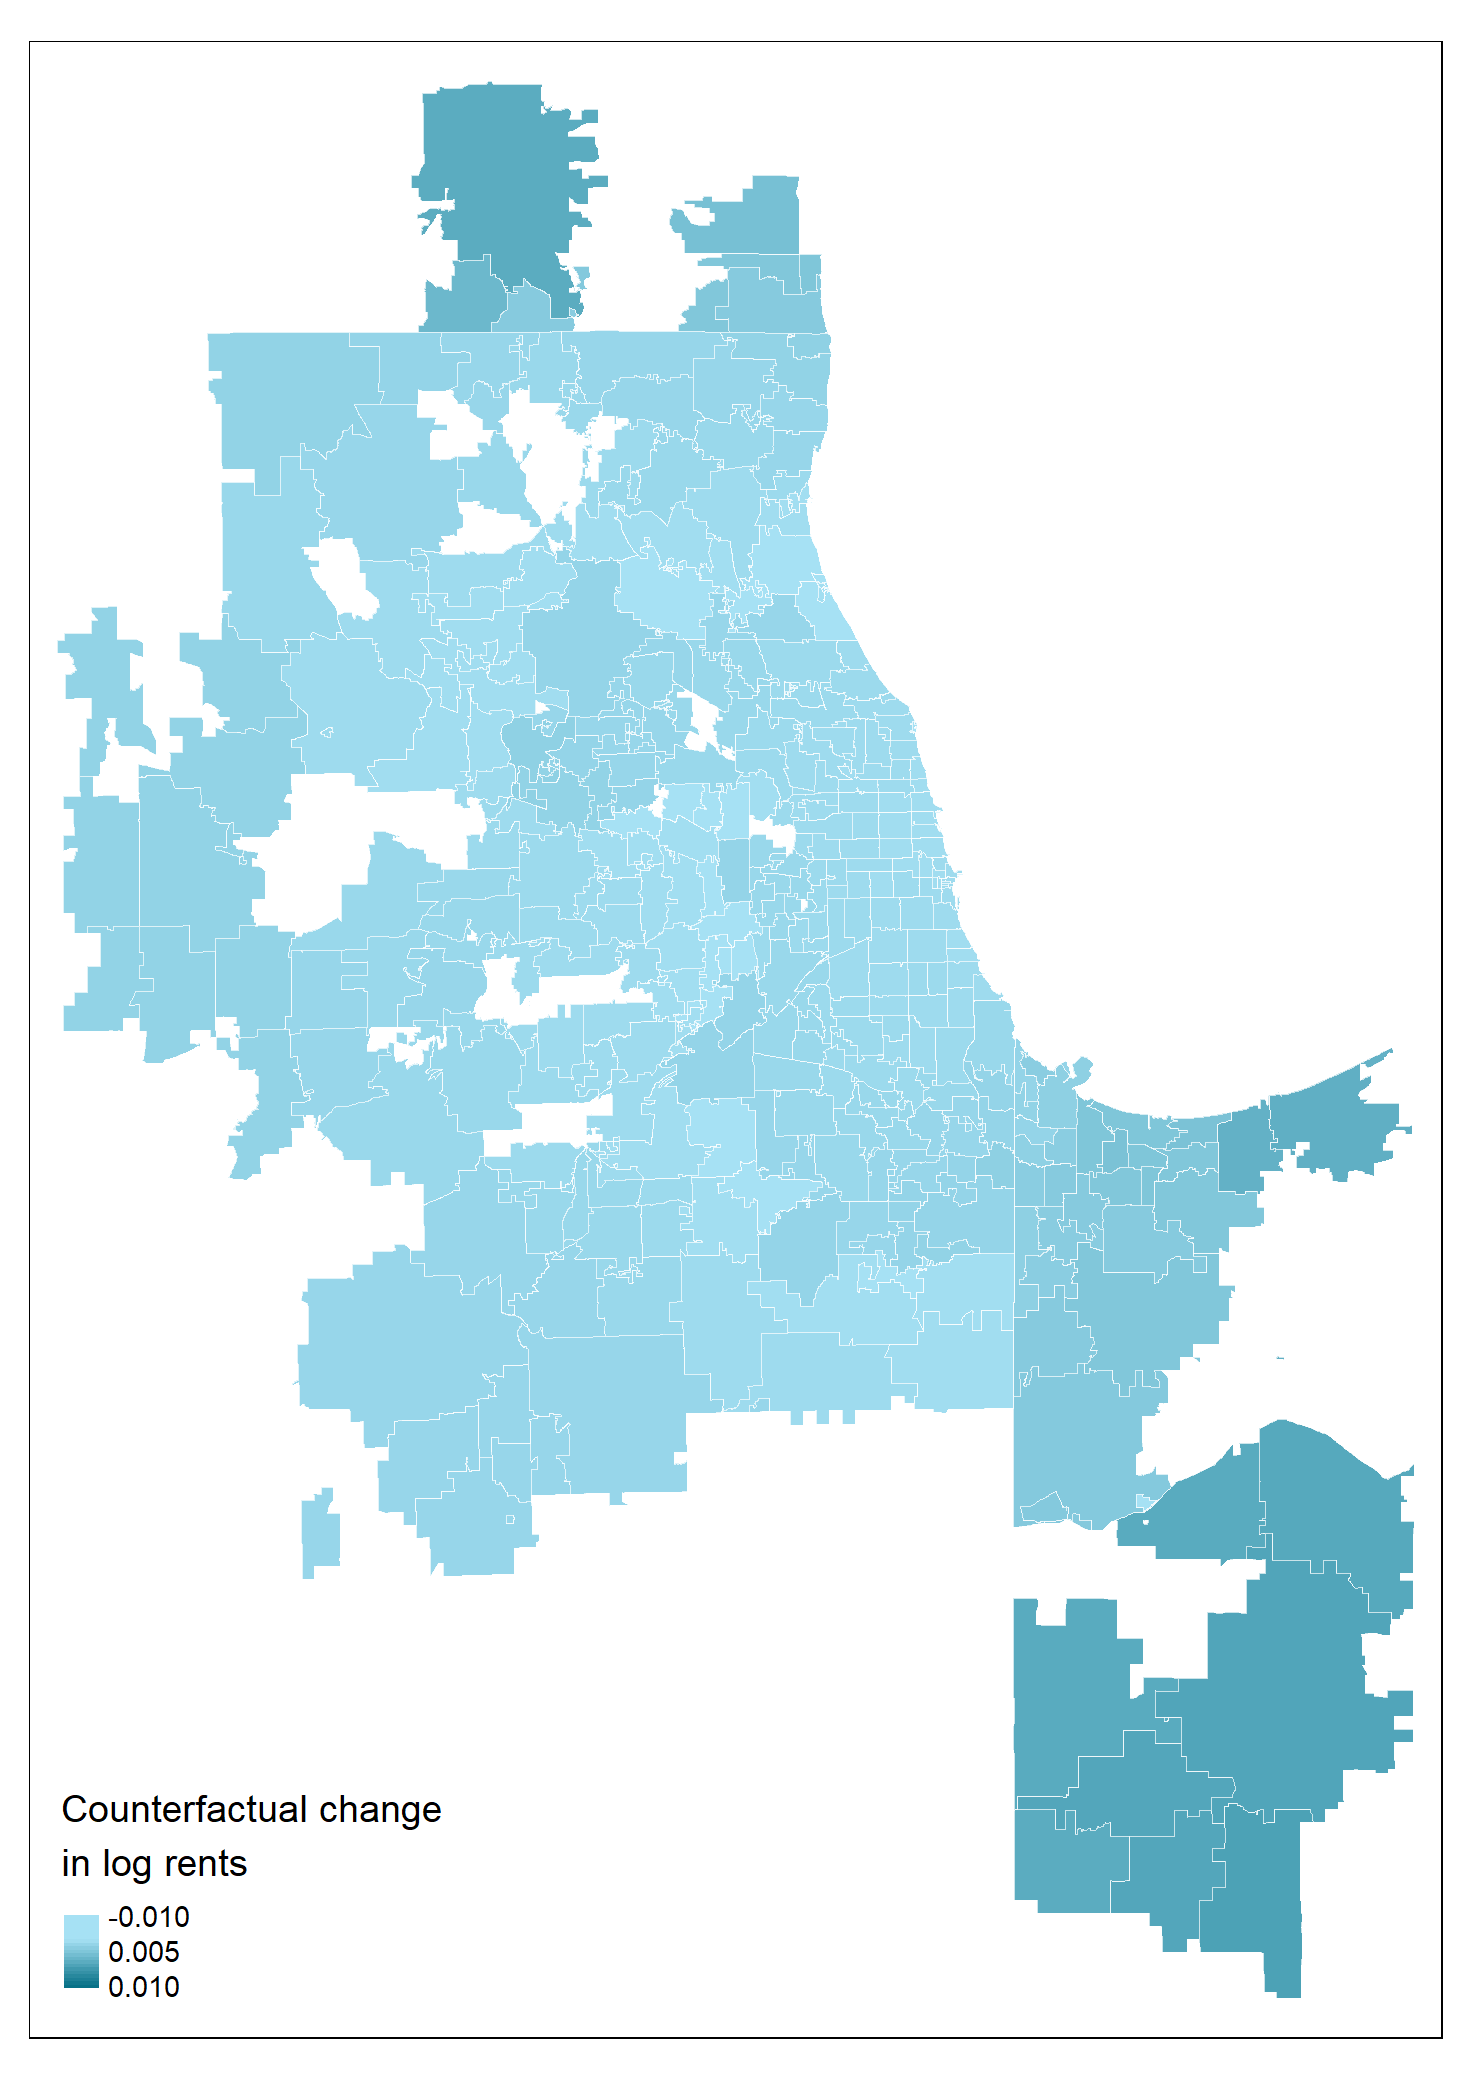
\includegraphics[width = 1\textwidth]
            {counterfactuals/output/chicago_d_ln_rents.png}
    \end{subfigure}%
    \begin{subfigure}{.35\textwidth}
        \caption*{Changes in log total wages}
        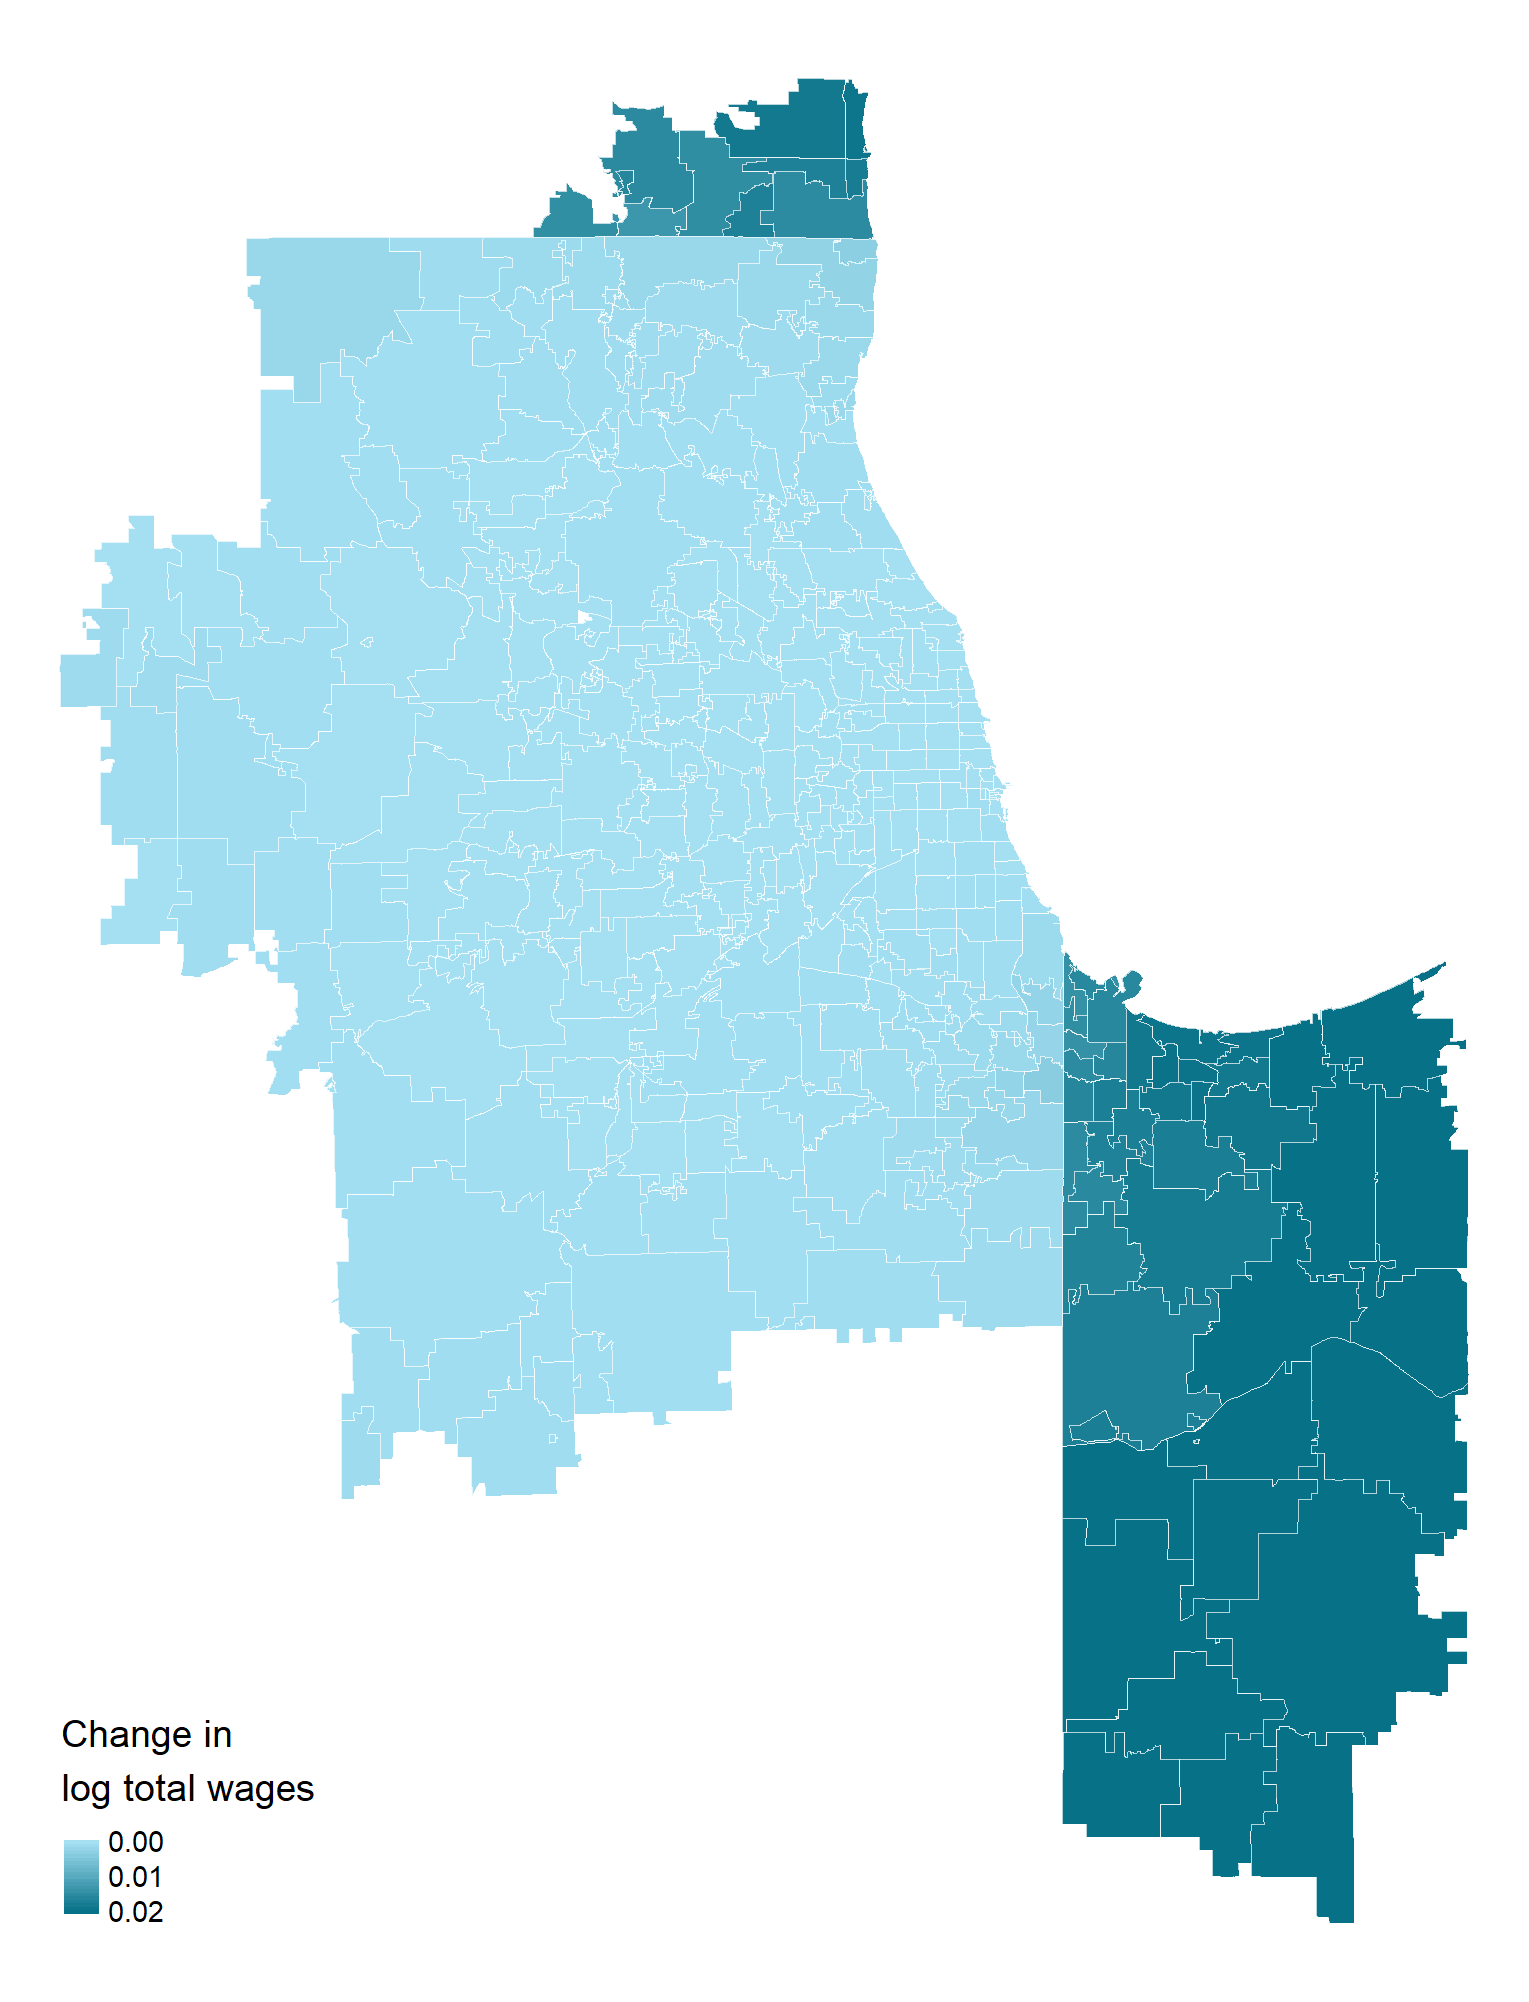
\includegraphics[width = 1\textwidth]
            {counterfactuals/output/chicago_d_ln_wagebill.png}
    \end{subfigure}

    \begin{minipage}{.95\textwidth} \footnotesize
        \vspace{3mm}
        Notes: 
        Data are from LODES and the minimum wage panel described in Section 
        \ref{sec:mw_construction}.
        The top figures maps the distribution of estimated landlord shares, 
        the bottom left figure maps estimated changes in log rents, and 
        the bottom right figure maps estimated changes in log total wages,
        for ZIP codes in the Chicago-Naperville-Elgin CBSA.
        The computations are based on a counterfactual increase to \$9 in the 
        federal MW in January 2020, holding constant other MW policies in their 
        December 2019 levels.
        The landlord share is defined as the ratio between the percent increase 
        in rents and the percent increase in total wages multipled by the share 
        of housing expenditure in the ZIP code.
        To estimate it we follow the procedure described in Section 
        \ref{sec:counterfactual}, assuming the following parameter values: 
        $\beta = 0.0546$, $\gamma = -0.0207$, $\varepsilon = 0.1083$, and 
        $s = 0.35$.
    \end{minipage}
\end{figure}

\clearpage
\begin{figure}[h!]
    \centering
    \caption{Estimates of the share pocketed by landlords by the relative 
             change in workplace MW to change in residence MW, urban ZIP codes}
    \label{fig:rho_by_decile_MW_gap}

	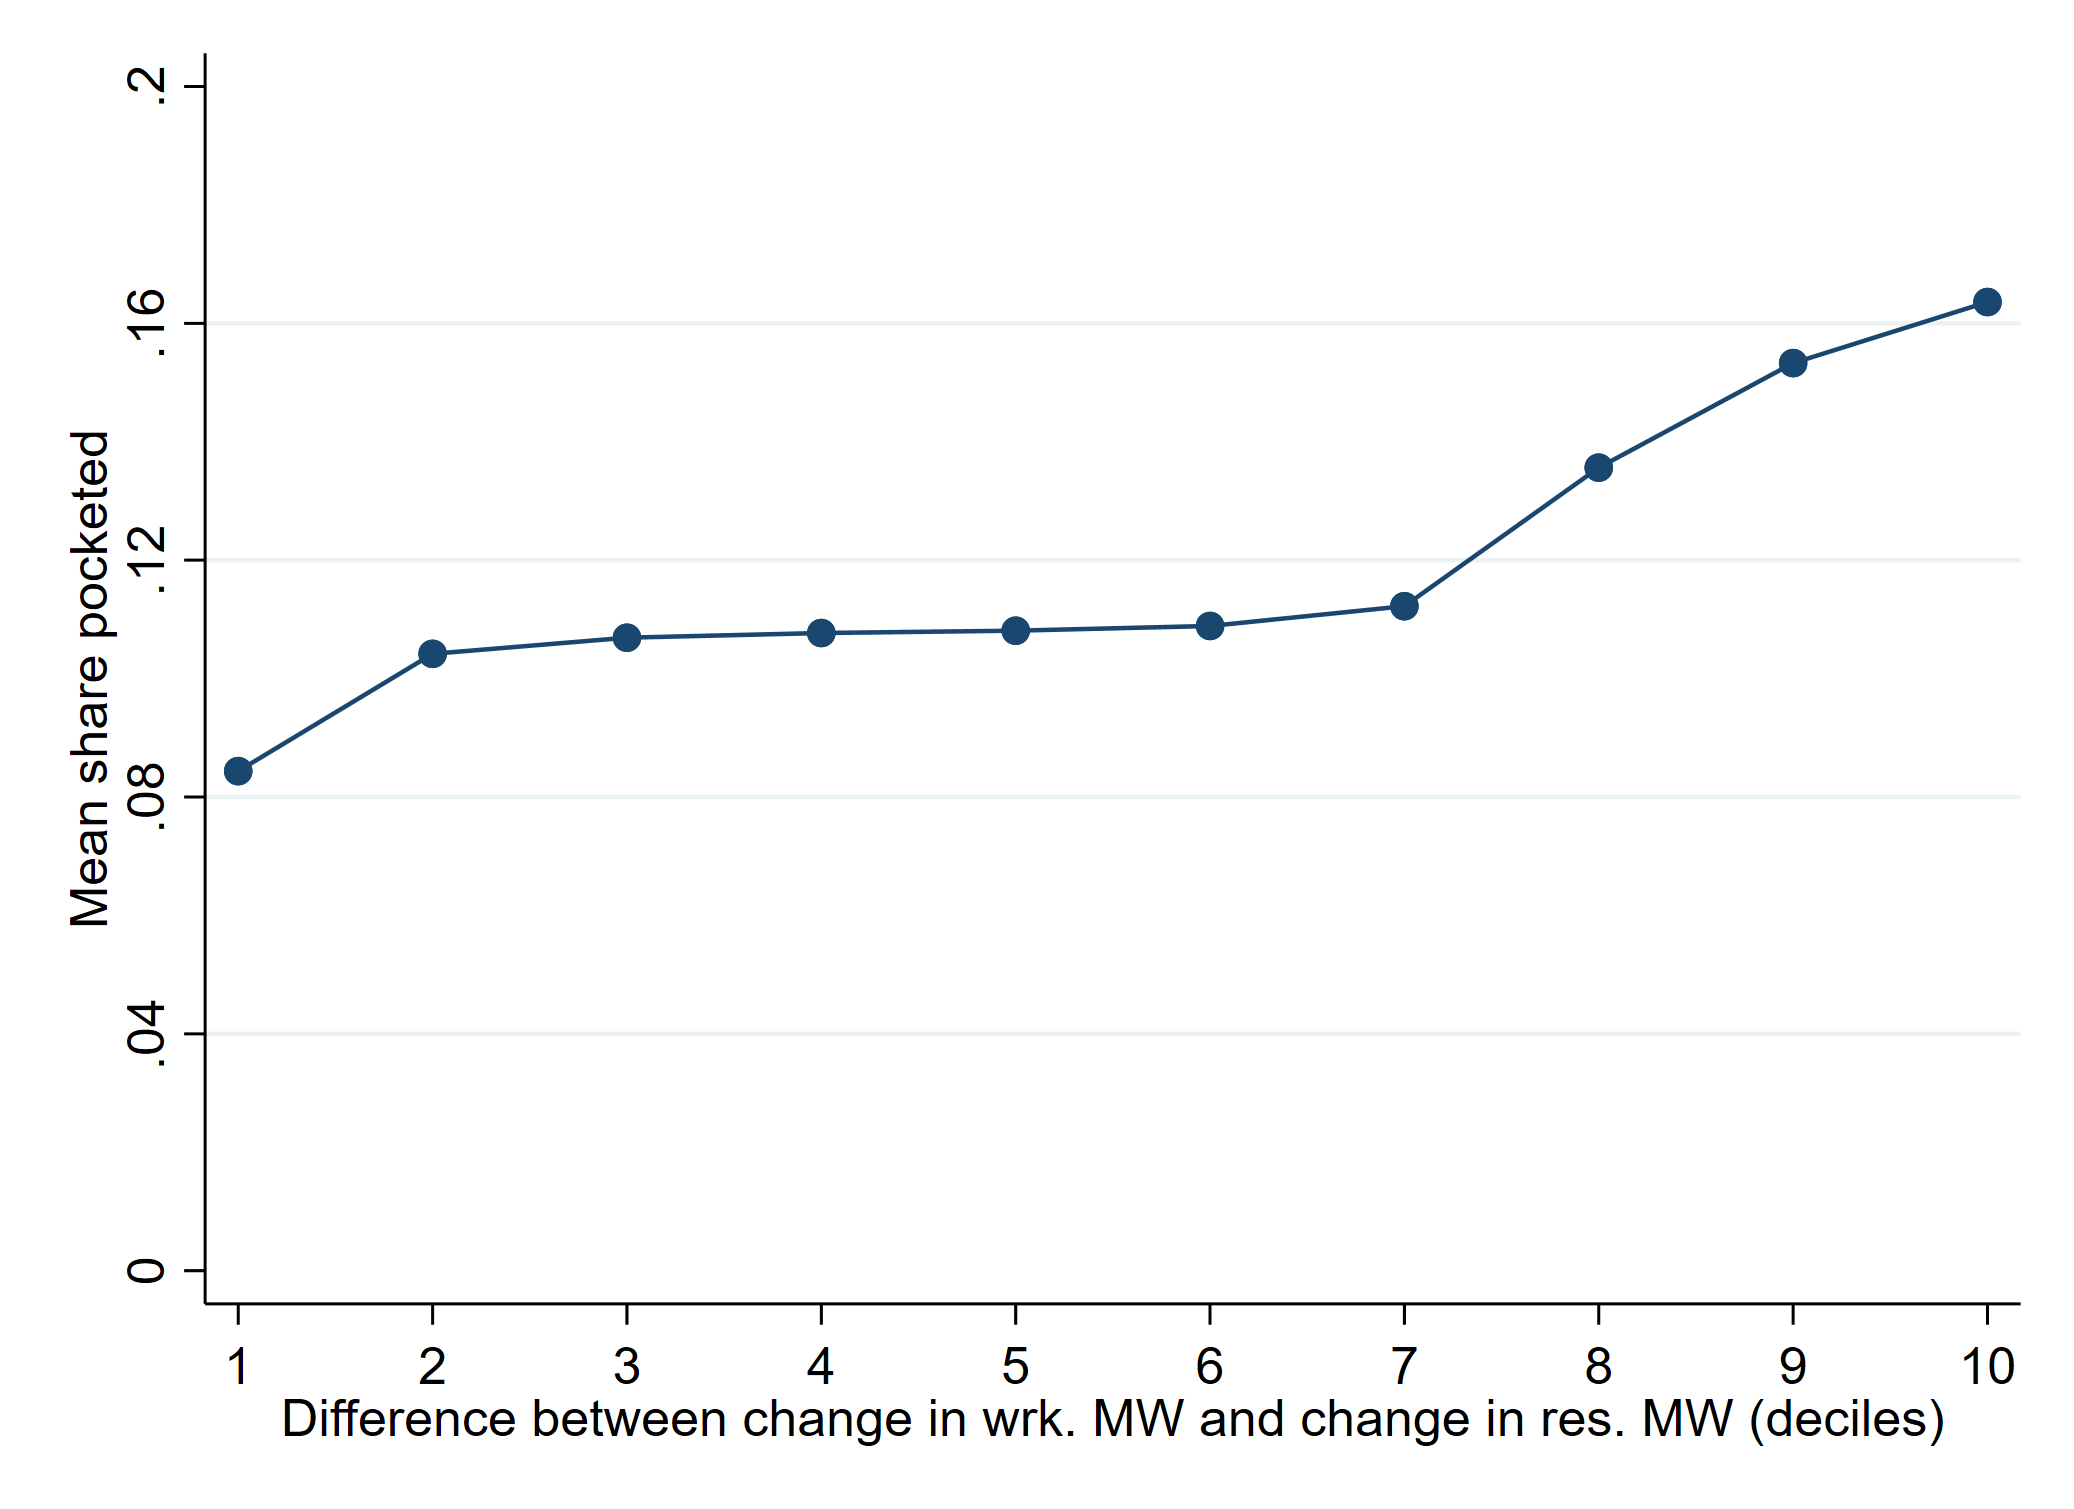
\includegraphics[width = 0.75\textwidth]{counterfactuals/output/deciles_diff.png}

    \begin{minipage}{.95\textwidth} \footnotesize
        \vspace{3mm}
        Notes:
        Data are from the minimum wage panel described in 
        Section \ref{sec:data_mw_panel} and from LODES.
        The figure shows the average estimate of the shares of the additional 
        income pocketed by landlords $\rho_i$ for each decile of the 
        difference $\Delta \mw_i^{\wkp} - \Delta \mw_i^{\res}$.
        Estimates for lower deciles correspond to ZIP codes where the increase 
        in residence MW was relatively large.
        The unit of observation is the urban ZIP code, where we define a ZIP code 
        as urban if it belongs to a CBSA with at least 80\% of its population 
        classified as urban by the 2010 Census.
        The share pocketed is defined as the ratio between the percent increase 
        in rents and the percent increase in total wages multiplied by the share 
        of housing expenditure in the ZIP code.
        To estimate it we follow the procedure described in Section 
        \ref{sec:counterfactual}, assuming the following parameter values: 
        $\beta = \betaCf$, $\gamma = \gammaCf$, $\varepsilon = \epsilonCf$, and 
        $s = 0.35$.
        The figure excludes ZIP codes located in the $\cbsaLowIncFedNine$ CBAs for which the average
        estimated change in log total wages was below 0.1\%.
    \end{minipage}
\end{figure}


\clearpage

\begin{table}[hbt!] \centering
    \caption{Descriptive statistics of different samples of ZIP codes}
    \label{tab:stats_zip_samples}
    \begin{tabular}{@{}lcccc@{}}
        \toprule
                                                        & \multicolumn{1}{c}{All ZIP codes} 
                                                        & \multicolumn{1}{c}{Urban ZIP codes} 
                                                        & \multicolumn{1}{c}{Zillow sample} 
                                                        & \multicolumn{1}{c}{Baseline sample}      \\ \midrule
        (a) Mean population, 2011                       & #2,# & #2,#  & #2,#  & #2,#    \\
        (b) Mean number of households, 2011             & #2,#  & #2,#  & #2,#  & #2,#      \\
        (c) Mean household size, 2011                   & #2,#    & #2,#  & #2,#  & #2,#         \\
        (d) Share urban ZIP codes, YYYY                 & #3#    & #3#   & #3#   & #3#          \\
        (e) Share renter households, 2011               & #3#    & #3#   & #3#   & #3#          \\
        (f) Share black population, 2011                & #3#    & #3#   & #3#   & #3#          \\
        (g) Share hispanic population, 2011             & #3#    & #3#   & #3#   & #3#          \\
        (h) Share households with wage income, 2010     & #3#    & #3#   & #3#   & #3#          \\
        (i) Share households with business income, 2010 & #3#    & #3#   & #3#   & #3#          \\
        (j) Mean wage income per household (\$), 2010   & #2,#   & #2,#  & #2,#  & #2,#         \\
        (k) Mean AGI per household (\$), 2010           & #2,#   & #2,#  & #2,#  & #2,#         \\
        (l) Mean 40th percentile 2BR apt.\ rent, 2012   & #2,#   & #2,#  & #2,#  & #2,#         \\
        (m) Min statutory MW, Feb.\ 2010                & #2,#    & #2,#  & #2,#  & #2,#         \\
        (n) Mean statutory MW, Feb.\ 2010               & #2,#    & #2,#  & #2,#  & #2,#         \\
        (o) Max statutory MW, Feb.\ 2010                & #2,#   & #2,#   & #2,#  & #2,#         \\
        (p) Number of ZIP codes                         & #0,#  & #0,#  & #0,#  & #0,#      \\ \bottomrule
    \end{tabular}

    \begin{minipage}{.95\textwidth} \footnotesize
        \vspace{2mm}
        Notes: The table shows characteristics of different samples of ZIP codes.
        The first column uses all valid USPS ZIP codes.
        The second restricts to urban ZIP codes, according to \textcite{MissouriCDC}.
        The third and fourth columns use the ZIP codes with valid SFCC rents 
        data, and the ones used in the baseline estimation, as described in
        Section \ref{sec:data}.
        Each row shows a given characteristic obtained from different a data 
        source.
        Rows (a)--(c) and (e)--(g) are constructed from the 2011 ACS \textcite{ACS}.
        Row (d) is based on an indicator obtained from \textcite{MissouriCDC}.
        Rows (h)--(k) are obtained from 2011 IRS ZIP code-level statiscs \textcite{IRS}.
        AGI is an acronym for the Average Gross Income of a ZIP code.
        Row (l) is obtained from SAFMR \textcite{hudSAFMR}.
        Rows (m)--(o) are computed using the panel of minimum wage levels 
        described in Section \ref{sec:data}.
    \end{minipage}
\end{table}

\clearpage
\begin{table}[hbt!] \centering
    \caption{Estimates of the effect of the MW on rents, baseline sample}
    \label{tab:static}
    \begin{tabular}{l*{4}{c}}
        \toprule
        & \multicolumn{1}{c}{\shortstack{Change wkp.\ MW\\$\Delta\mw_{it}^{\wkp}$}}
            & \multicolumn{3}{c}{\shortstack{Change log rents\\$\Delta r_{it}$}} \\ \cmidrule(lr){2-2}\cmidrule(lr){3-5}
                                           & (1)   & (2)   & (3)   & (4)            \\ \midrule
        Change residence MW 
                  $\Delta\mw_{it}^{\res}$  &  0.8627  &  0.0372  &       &  -0.0219     \\
                                           & (0.0374) & (0.0145) &       & (0.0175)    \\
        Change workplace MW 
                   $\Delta\mw_{it}^{\wkp}$ &       &       &  0.0449  & 0.0685      \\
                                           &       &       & (0.0156) & (0.0288)    \\ \midrule
        Sum of coefficients                &       &       &       &  0.0466     \\
                                           &       &       &       & (0.0158)    \\ \midrule
        County-quarter economic controls   &  Yes  & Yes   & Yes   & Yes      \\
        P-value equality                   &       &       &       & 0.0514      \\
        R-squared                          &  0.9444  &  0.0212  &  0.0213  & 0.0213      \\
        Observations                       & 80,241  & 80,241  & 80,241  & 80,241     \\\bottomrule
    \end{tabular}

    \begin{minipage}{.95\textwidth} \footnotesize
        \vspace{2mm}
        Notes:
        Data are from the baseline estimation sample described in Section 
        \ref{sec:data_final_panel}.
        Column (1) shows the results of a regression of the workplace MW measure
        on the residence MW measure.
        Column (2) through (4) show the results of regressions of the log of 
        median rents per square foot on our MW-based measures.
        All regressions are estimated in first differences and include 
        time-period fixed effects and economic controls that vary at the 
        county and month levels.
        The measure of rents per square foot corresponds to the Single Family, 
        Condominium and Cooperative houses from Zillow.
        The residence MW is defined as the log statutory MW in the same ZIP code.
        The workplace MW is defined as the statutory MW where the average 
        resident of the ZIP code works, constructed using LODES 
        origin-destination data.
        Economic controls from the QCEW include the log of the average wage, 
        the log of employment, and the log of the establishment count from the 
        sectors ``Information'', ``Financial activities'', and ``Professional
        and business services''.
        Standard errors in parentheses are clustered at the state level.
    \end{minipage}
\end{table}

\clearpage
\begin{table}
    \caption{Static model, sample selection concerns}
    \label{tab:static_sample}

    \begin{tabular}{@{}lcccccc@{}}
        \toprule
                                             & \multicolumn{6}{c}{Change log rents}                                     \\ \cmidrule(l){2-7} 
                                             & \shortstack{Baseline\\(1)}       & \shortstack{Baseline\\Reweighted (2)}
                                             & \shortstack{Unbalanced\\(3)}     & \shortstack{Unbalanced\\Reweighted (4)}
                                             & \shortstack{Fully-balanced\\(5)} & \shortstack{Fully-balanced\\Reweighted (6)}  \\ \midrule
        Change residence minimum wage        & -0.0196      & -0.0071        & -0.0223       & -0.0142      & -0.0185     & 0.0041            \\
                                             & (0.0169)    & (0.0176)      & (0.0198)     & (0.0190)    & (0.0199)   & (0.0160)          \\
        Change workplace minimum wage        & 0.0531      & 0.0455        & 0.0435       & 0.0347      & 0.0666     & 0.0482            \\
                                             & (0.0284)    & (0.0304)      & (0.0304)     & (0.0342)    & (0.0310)   & (0.0295)          \\ \midrule
        P-value equality                     & 0.1074      & 0.2649        & 0.1820       & 0.3474      & 0.0916     & 0.3255            \\
        R-squared                            & 0.0208      & 0.0204        & 0.0160       & 0.0146      & 0.0214     & 0.0204            \\
        Observations                         & 131,306     & 125,425       & 193,081      & 184,987     & 78,853    & 75,388           \\ \bottomrule
    \end{tabular}

    \begin{minipage}{.95\textwidth} \footnotesize
        \vspace{2mm}
        Notes: 
    \end{minipage}
\end{table}

\clearpage
\begin{landscape}
\begin{table}[ht!]
    \centering
    \caption{Estimates of the effect of the MW on rents, robustness}
    \label{tab:robustness}
        
    \begin{tabular}{@{}lccccc@{}}
        \toprule
                                                         & \shortstack{Change wkp.\\MW $\Delta\mw_{it}^{\wkp}$} 
                                                         & \multicolumn{3}{c}{\shortstack{Change log rents\\$\Delta r_{it}$}} 
                                                         &                                                                           \\ \cmidrule(lr){2-2}\cmidrule(lr){3-5}
                                                             & \multicolumn{1}{c}{\shortstack{Change res.\\MW $\Delta\mw_{it}^{\res}$}}
                                                             & \multicolumn{1}{c}{\shortstack{Change res.\\MW $\Delta\mw_{it}^{\res}$}}
                                                             & \multicolumn{1}{c}{\shortstack{Change wkp.\\MW $\Delta\mw_{it}^{\wkp}$}} 
                                                             & \shortstack{Sum of\\coefficients}
                                                             & N                                                                      \\ \midrule
        $\quad$(a) Baseline                                  &  0.8648  &  -0.0204  &  0.0545  &  0.0342  & 131,383 \\
                                                             & (0.0300) & (0.0169) & (0.0283) & (0.0155) &      \\
        \textit{Panel A: Vary specification}                 &       &       &       &       &      \\
        $\quad$(b) No controls                               &  0.8656  &  -0.0184  &  0.0523  &  0.0339  & 132,255 \\
                                                             & (0.0299) & (0.0173) & (0.0288) & (0.0159) &      \\
        $\quad$(c) County $\times$ time FE                   &  0.2851  &  -0.0256  &  0.0315  &  0.0059  & 123,674 \\
                                                             & (0.0397) & (0.0399) & (0.0604) & (0.0500) &      \\
        $\quad$(d) CBSA $\times$ time FE                     &  0.5073  &  -0.0373  &  0.0908  &  0.0535  & 128,240 \\
                                                             & (0.0341) & (0.0289) & (0.0592) & (0.0321) &      \\
        $\quad$(e) State $\times$ time FE                    &  0.5284  &  0.0135  &  -0.0175  &  -0.0040  & 131,726 \\
                                                             & (0.0591) & (0.0213) & (0.0444) & (0.0268) &      \\
        $\quad$(f) ZIP code-specific linear trend            &  0.8628  &  -0.0216  &  0.0561  &  0.0345  & 131,383 \\
                                                             & (0.0308) & (0.0157) & (0.0272) & (0.0147) &      \\
        \textit{Panel B: Vary workplace MW measure}          &       &       &       &       &      \\
        $\quad$(g) 2014 commuting shares                     &  0.8658  &  -0.0202  &  0.0542  &  0.0341  & 131,383 \\
                                                             & (0.0309) & (0.0186) & (0.0296) & (0.0154) &      \\
        $\quad$(h) 2018 commuting shares                     &  0.8660  &  -0.0209  &  0.0550  &  0.0342  & 131,383 \\
                                                             & (0.0305) & (0.0175) & (0.0293) & (0.0155) &      \\
        $\quad$(i) Time-varying commuting shares             &  0.8794  &  -0.0286  &  0.0649  &  0.0362  & 115,378 \\
                                                             & (0.0303) & (0.0195) & (0.0301) & (0.0161) &      \\
        $\quad$(j) 2017 commuting shares, low-income workers &  0.8588  &  -0.0296  &  0.0656  &  0.0360  & 131,383 \\
                                                             & (0.0297) & (0.0207) & (0.0339) & (0.0161) &      \\
        $\quad$(k) 2017 commuting shares, young workers      &  0.8615  &  -0.0312  &  0.0673  &  0.0361  & 131,383 \\
                                                             & (0.0308) & (0.0167) & (0.0290) & (0.0155) &      \\ \bottomrule
    \end{tabular}

    \begin{minipage}{.95\linewidth} \footnotesize
        \vspace{2mm}
        Notes: 
        Data are from the baseline estimation sample described in Section 
        \ref{sec:data_final_panel}.
        Each row of the table shows two estimations on the same sample of ZIP 
        codes and months.
        The first column shows the results of a regression of the change in the 
        workplace MW measure on the change in the residence MW measure.
        The second through fourth columns show the results of a regression of 
        the change in log rents on the change in the residence MW and the 
        workplace MW, with the fifth column showing the sum of the coefficients 
        on the MW measures.
        The rents variable corresponds to the median rent per square foot in
        the Zillow data.
        Row (a) repeats the results of Table \ref{tab:static}, including fixed
        effects for each year month and economic controls at the 
        county $\times$ quarter level.
        Specifications in Panel A vary the set of controls included in the 
        regression relative to row (a).
        Row (f) includes ZIP code fixed effects in the first-differenced model,
        which in the level model can be interpreted as a ZIP-code specific 
        linear trend.
        Specifications in Panel B vary the commuting shares used to construct 
        the workplace MW measure relative to row (a).
        Standard errors in parenthesis are clustered at the state level.
    \end{minipage}
\end{table}
\end{landscape}

\clearpage
\begin{table}[hbt!]
    \centering
    \caption{Effect of an increase in federal MW to \$9 in January 2020, urban ZIP codes}
    \label{tab:counterfactuals_fed_9usd}

    \begin{tabular}{@{}lccccc@{}}
        \toprule
                            &   & \multicolumn{2}{c}{Average change in...}
                                & \multicolumn{2}{c}{Avg.\ landlord share}       \\ \cmidrule(lr){3-4}\cmidrule(lr){5-6}
                            & N & Res.\ MW & Wkp.\ MW
                            & $s = $ 0.25  & $s = $ 0.45                           \\ \midrule
        Effect in ZIP codes with...          &      &       &       &     &      \\
        $\quad$previous MW $\leq\$9\quad$    & 17,185 &  0.161 & 0.153  & 0.075 &  0.136   \\
        $\quad$previous MW $>\$9\quad$       & 5,321 &  0.000 & 0.005  & 0.126 & 0.227    \\ \bottomrule
    \end{tabular}
    
    \begin{minipage}{.95\textwidth} \footnotesize
        \vspace{2mm}
        Notes: 
        Data are from LODES and the minimum wage panel described in Section 
        \ref{sec:mw_construction}.
        The table shows averages of the ZIP code-specific landlord share ($\rho_i$),
        defined as the ratio of the increase in income to the increase in rents.
        Increases in income and rents are simulated following the procedure
        described in Section \ref{sec:counterfactual}, where we assume 
        an increase in the federal MW to \$9.
        We assume the following parameter values: 
        $\beta = 0.0546$, $\gamma = -0.0207$, $\varepsilon = 0.1083$, and 
        $s\in\{0.25, 0.45\}$.
        We carry out our computations only for urban ZIP codes, defined as 
        those that belong to a CBSA with at least 80\% of urban population
        according to the 2010 census.
    \end{minipage}
\end{table}

%%%%%%%%%%%%%%%%%%%%%%%%%%%%%%%%%%%%%%%%%%%%%%%%%%%%%%%%%%%%%%%%%%%%%%%%%%%%%%%%
%%%%                             APPENDIX                                   %%%%
%%%%%%%%%%%%%%%%%%%%%%%%%%%%%%%%%%%%%%%%%%%%%%%%%%%%%%%%%%%%%%%%%%%%%%%%%%%%%%%%

\clearpage

\section*{\centering{Appendix}}
\vspace{5mm}

\appendix

\renewcommand\thetable{\arabic{table}} 
\renewcommand\thefigure{\arabic{figure}}
\renewcommand{\tablename}{Appendix Table}
\renewcommand{\figurename}{Appendix Figure}
\setcounter{table}{0}
\setcounter{figure}{0}

%%%%%%%%%%%%%%%%%%%%%%%%%%%%%%%%%%%%%%%%%%%%%%%%%%%%%%%%%%%%%%%%%%%%%%%%%%%%%%%%%
%%%%%                           ONLINE APPENDIX                              %%%%
%%%%%%%%%%%%%%%%%%%%%%%%%%%%%%%%%%%%%%%%%%%%%%%%%%%%%%%%%%%%%%%%%%%%%%%%%%%%%%%%%
%%%%%%%%%%%%%%%%%%%%%%%%%%%%%%%%%%%%%%%%%%%%%%%%%%%%%%%%%%%%%%%%%%%%%%%%%%%%%%%%%
\section{Appendix Tables}

\begin{table}[h!]
	\caption{Extended Descriptive Statistics of Estimating Panel}
	\label{tab:estimating_panel_stats_long}
	\centering
	
% Table created by stargazer v.5.2.2 by Marek Hlavac, Harvard University. E-mail: hlavac at fas.harvard.edu
% Date and time: Mon, Nov 30, 2020 - 11:59:19 AM
\begin{tabular}{@{\extracolsep{5pt}}lccccc} 
\\[-1.8ex]\hline 
\hline \\[-1.8ex] 
Statistic & \multicolumn{1}{c}{N} & \multicolumn{1}{c}{Mean} & \multicolumn{1}{c}{St. Dev.} & \multicolumn{1}{c}{Min} & \multicolumn{1}{c}{Max} \\ 
\hline \\[-1.8ex] 
Statutory MW & 156,600 & 8.08 & 1.21 & 7 & 16 \\ 
Experienced MW (total jobs) & 156,600 & 8.06 & 1.20 & 6.29 & 14.98 \\ 
Experienced MW (low inc.) & 156,600 & 8.06 & 1.20 & 5.81 & 15.02 \\ 
Experienced MW (young) & 156,600 & 8.06 & 1.20 & 6.19 & 15.07 \\ 
Median rent psqft. 2BR & 24,789 & 1.96 & 0.97 & 0.53 & 6.51 \\ 
Median rent psqft. MFR5plus & 37,588 & 1.96 & 1.05 & 0.55 & 6.69 \\ 
Median rent psqft.SFCC & 113,375 & 1.27 & 0.83 & 0.47 & 7.25 \\ 
Median rent SFCC & 125,644 & 1,651.10 & 702.99 & 595.00 & 6,595.00 \\ 
Avg. wage Fin. activities & 152,334 & 1,561.78 & 965.27 & 0.00 & 9,557.00 \\ 
Employment Fin. activities & 152,334 & 59,554.22 & 75,796.09 & 0.00 & 397,839.00 \\ 
Estab. count Fin. activities & 152,334 & 5,103.83 & 5,200.06 & 31.00 & 30,405.00 \\ 
Avg. wage Prof. and bus. serv. & 152,334 & 1,252.94 & 434.75 & 226.00 & 4,727.00 \\ 
Employment Prof. and bus. serv. & 152,334 & 134,280.40 & 143,863.40 & 329.00 & 640,795.00 \\ 
Estab. count Prof. and bus. serv. & 152,334 & 9,999.11 & 9,479.67 & 60.00 & 56,758.00 \\ 
Avg. wage Information & 152,334 & 1,505.07 & 619.82 & 0.00 & 7,380.00 \\ 
Employment Information & 152,334 & 21,041.80 & 35,131.53 & 0.00 & 238,776.00 \\ 
Estab. count Information & 152,334 & 920.54 & 1,381.95 & 4.00 & 13,271.00 \\ 
\hline \\[-1.8ex] 
\end{tabular} 

	\begin{minipage}{0.95\textwidth} \footnotesize
		\vspace{3mm} 
		\textit{Notes}: The table shows summary statistics of our baseline estimating panel.
		Variables included are the statutory and experienced MW, constructed using different
		sets of weights as explained in \autoref{sec:mw_construction}; median monthly rents 
		per square foot in the categories 2 bedroom (2BR), multi family houses with 5 or more 
		units (MFR5plus), and SFCC, and absolute median rents for the SFCC category, all taken
		directly from Zillow; and average weekly wage, employment and establishment count 
		for three industries used in our estimation, obtained from the QCEW.
	\end{minipage}
\end{table}

\clearpage
\begin{table}[h!] \centering
	\caption{Comparison of level and first difference models}
	\label{tab:level_auto}
	{
\def\sym#1{\ifmmode^{#1}\else\(^{#1}\)\fi}
\begin{tabular}{l*{2}{c}}
\hline\hline
          &\multicolumn{1}{c}{(1)}&\multicolumn{1}{c}{(2)}\\
          &\multicolumn{1}{c}{Level}&\multicolumn{1}{c}{First Difference}\\
\hline
$\ln(MW)$ &   0.0369         &                  \\
          & (0.0688)         &                  \\
[1em]
$\Delta\ln(MW)$&                  &   0.0259\sym{*}  \\
          &                  & (0.0129)         \\
\hline
P-value autocorrelation test&                  &   0.0000         \\
Observations&  113,375         &  112,232         \\
\hline\hline
\end{tabular}
}

	\begin{minipage}{0.95\textwidth} \footnotesize
		\vspace{3mm} 
		\textit{Notes}: In column (1) we report results from a regression of median SFCC rent on 
		MW levels with ZIP code and year-month fixed effects. In column (2), we report the same 
		regression but in first differences (note that the ZIP code  fixed effects drop out). For 
		the model in first differences, we also report an AR 1 auto-correlation test. We proceed 
		as in \parencite[][section 10.6.3]{wooldridge2010}. We compute the residuals of the model 
		estimated in column (2), and we regress those residuals on their lag. We call that 
		coefficient $\rho$. The model in levels is efficient assuming no auto-correlation of the 
		error term, which would imply that the residuals of the first difference model are 
		auto-correlated with $\rho = -0.5$. We report the p-value of testing that hypothesis.
	\end{minipage} 
\end{table}

\clearpage
\begin{table}[h!]
	\caption{Results from Static Model Controlling for Parametric Trends}
	\label{tab:did_trend}
	\centering
	\resizebox{1\textwidth}{!}{
	{
\def\sym#1{\ifmmode^{#1}\else\(^{#1}\)\fi}
\begin{tabular}{l*{6}{c}}
\hline\hline
          &\multicolumn{1}{c}{(1)}         &\multicolumn{1}{c}{(2)}         &\multicolumn{1}{c}{(3)}         &\multicolumn{1}{c}{(4)}         &\multicolumn{1}{c}{(5)}         &\multicolumn{1}{c}{(6)}         \\
\hline
$\Delta \ln \underline{w}_{ict}$&   0.0260\sym{**} &   0.0257\sym{**} &   0.0255\sym{**} &   0.0258\sym{**} &   0.0248\sym{**} &   0.0242\sym{**} \\
          & (0.0128)         & (0.0120)         & (0.0117)         & (0.0124)         & (0.0116)         & (0.0111)         \\
\hline
\vspace{-2mm}&                  &                  &                  &                  &                  &                  \\
Zipcode-specifc linear trend&       No         &      Yes         &      Yes         &       No         &      Yes         &      Yes         \\
Zipcode-specific quadratic trend&       No         &       No         &      Yes         &       No         &       No         &      Yes         \\
Local economy controls&       No         &       No         &       No         &      Yes         &      Yes         &      Yes         \\
R-squared &    0.022         &    0.024         &    0.026         &    0.022         &    0.024         &    0.027         \\
Observations&  112,232         &  112,232         &  112,232         &  107,814         &  107,814         &  107,814         \\
\hline\hline
\end{tabular}
}

	}
	\begin{minipage}{0.95\textwidth} \footnotesize
		\vspace{3mm} 
		\textit{Notes}: The table reports coefficients from versions of \autoref{eq:did} 
		estimated on the balanced panel of ZIP code-months described in \autoref{sec:data}. 
		The dependent variable is the difference in the natural logarithm of median	rents 
		per	square foot in the Single Family, Condos and Condominiums category in Zillow, 
		whereas the main independent variable is the difference in the natural logarithm
		of the statutory minimum wage. All columns include controls for monthly date fixed 
		effects. In addition, column (2) controls for ZIP code-specific linear trend (which 
		in a differenced model amounts to including a ZIP code fixed effect), and column (3) 
		controls for ZIP code-specific linear and quadratic trends (which amount to 
		including a ZIP code fixed effect and a ZIP code-specific trend). Columns (4), (5), 
		and (6) replicate the specifications presented in columns (1)-(3) respectively, while 
		including economic controls from the industries ``Professional and business services'', 
		``Information'', and ``Financial activities'' from the QCEW. Economic controls are 
		the difference in the natural logarithm of average weekly wages, the difference in 
		the natural logarithm of employment, and the difference in the natural logarithm 
		of number of establishments. Wages and employment vary at the county-month level,
		whereas establishment count varies at the country-quarter level.
		Standard errors clustered at the state level are reported in parenthesis. Significance 
		codes: *** $p < 0.01$, ** $p < 0.05$, * $p < 0.1$.
	\end{minipage}
\end{table}

\clearpage
\begin{table}[h!]
	\caption{Complete Results of Dynamic Model}
	\label{tab:dynamic_lags_leads_main}
	\centering
	{
\def\sym#1{\ifmmode^{#1}\else\(^{#1}\)\fi}
\begin{tabular}{l*{5}{c}}
\hline\hline
          &\multicolumn{1}{c}{(1)}         &\multicolumn{1}{c}{(2)}         &\multicolumn{1}{c}{(3)}         &\multicolumn{1}{c}{(4)}         &\multicolumn{1}{c}{(5)}         \\
\hline
$\Delta \ln \underline{w}_{ic,t-5}$&  -0.0148         &  -0.0144         &  -0.0144         &  -0.0146         &  -0.0144         \\
          & (0.0090)         & (0.0089)         & (0.0089)         & (0.0090)         & (0.0089)         \\
[1em]
$\Delta \ln \underline{w}_{ic,t-4}$&  -0.0024         &  -0.0019         &  -0.0020         &  -0.0022         &  -0.0019         \\
          & (0.0116)         & (0.0116)         & (0.0115)         & (0.0116)         & (0.0115)         \\
[1em]
$\Delta \ln \underline{w}_{ic,t-3}$&   0.0011         &   0.0005         &   0.0007         &   0.0004         &  -0.0002         \\
          & (0.0092)         & (0.0094)         & (0.0092)         & (0.0091)         & (0.0092)         \\
[1em]
$\Delta \ln \underline{w}_{ic,t-2}$&   0.0060         &   0.0063         &   0.0062         &   0.0060         &   0.0064         \\
          & (0.0116)         & (0.0118)         & (0.0116)         & (0.0115)         & (0.0117)         \\
[1em]
$\Delta \ln \underline{w}_{ic,t-1}$&  -0.0002         &  -0.0004         &  -0.0005         &   0.0000         &  -0.0005         \\
          & (0.0123)         & (0.0123)         & (0.0124)         & (0.0122)         & (0.0123)         \\
[1em]
$\Delta \ln \underline{w}_{ic,t}$&   0.0271\sym{**} &   0.0257\sym{**} &   0.0259\sym{**} &   0.0269\sym{**} &   0.0259\sym{**} \\
          & (0.0126)         & (0.0123)         & (0.0124)         & (0.0126)         & (0.0124)         \\
[1em]
$\Delta \ln \underline{w}_{ic,t+1}$&   0.0136\sym{*}  &   0.0146\sym{**} &   0.0142\sym{*}  &   0.0135\sym{*}  &   0.0146\sym{*}  \\
          & (0.0072)         & (0.0072)         & (0.0072)         & (0.0072)         & (0.0072)         \\
[1em]
$\Delta \ln \underline{w}_{ic,t+2}$&  -0.0070         &  -0.0066         &  -0.0064         &  -0.0068         &  -0.0064         \\
          & (0.0133)         & (0.0133)         & (0.0132)         & (0.0133)         & (0.0132)         \\
[1em]
$\Delta \ln \underline{w}_{ic,t+3}$&   0.0036         &   0.0045         &   0.0047         &   0.0031         &   0.0040         \\
          & (0.0081)         & (0.0078)         & (0.0078)         & (0.0079)         & (0.0077)         \\
[1em]
$\Delta \ln \underline{w}_{ic,t+4}$&   0.0108         &   0.0093         &   0.0104         &   0.0107         &   0.0096         \\
          & (0.0069)         & (0.0066)         & (0.0064)         & (0.0069)         & (0.0065)         \\
[1em]
$\Delta \ln \underline{w}_{ic,t+5}$&   0.0086         &   0.0095         &   0.0099         &   0.0088         &   0.0099         \\
          & (0.0069)         & (0.0065)         & (0.0065)         & (0.0067)         & (0.0065)         \\
\hline
\vspace{-2mm}&                  &                  &                  &                  &                  \\
Cumulative effect&    0.057         &0.057\sym{*}         &0.059\sym{*}         &    0.056         &0.058\sym{*}         \\
          &  (0.035)         &  (0.034)         &  (0.034)         &  (0.034)         &  (0.034)         \\
\hline    &                  &                  &                  &                  &                  \\
P-value no pretrends&    0.568         &    0.612         &    0.599         &    0.594         &    0.629         \\
Wage controls&       No         &      Yes         &       No         &       No         &      Yes         \\
Employment controls&       No         &       No         &      Yes         &       No         &      Yes         \\
Establishment-count controls&       No         &       No         &       No         &      Yes         &      Yes         \\
R-squared &    0.022         &    0.022         &    0.022         &    0.022         &    0.022         \\
Observations&  106,446         &  105,463         &  105,463         &  106,160         &  105,463         \\
\hline\hline
\end{tabular}
}

	\begin{minipage}{0.95\textwidth} \footnotesize
		\vspace{3mm} 
		\textit{Notes}: The table reports coefficients from versions of 
		\autoref{eq:leads_lags} estimated on the balanced panel of ZIP code-months
		described in \autoref{sec:data}. The dependent variable is the difference in 
		the natural logarithm of median	rents per square foot in the Single Family, Condos 
		and Condominiums category in Zillow. We report coefficients of five leads and lags 
		of the difference in the logarithm of the statutory minimum wage. All columns 
		control for monthly date fixed effects. In addition, columns (2) to (5) include 
		economic controls from the industries ``Professional and business services'', 
		``Information'', and ``Financial activities'' from the QCEW. Wage controls are 
		the difference in the natural logarithm of average weekly wages, employment 
		controls are the difference in the natural logarithm of employment, and 
		establishment count controls refer to the difference in the natural logarithm 
		of number of establishments. Wages and employment vary at the county-month level,
		whereas establishment count varies at the country-quarter level. The row 
		``Cumulative Effect'' shows the cumulative 	sum of the sum of all coefficients. 
		Standard errors clustered at the state level are reported in parenthesis. 
		Significance codes: *** $p < 0.01$, ** $p < 0.05$, * $p < 0.1$.
	\end{minipage}
\end{table}


\begin{table}[h!]\centering
	\caption{Complete Results for Static, Dynamic, and Panel models}
	\label{tab:horse_race_ab}
	\resizebox{\textwidth}{!}{
	{
\def\sym#1{\ifmmode^{#1}\else\(^{#1}\)\fi}
\begin{tabular}{l*{8}{c}}
\hline\hline
          &\multicolumn{1}{c}{(1)}&\multicolumn{1}{c}{(2)}&\multicolumn{1}{c}{(3)}&\multicolumn{1}{c}{(4)}&\multicolumn{1}{c}{(5)}&\multicolumn{1}{c}{(6)}&\multicolumn{1}{c}{(7)}&\multicolumn{1}{c}{(8)}\\
          &\multicolumn{1}{c}{DiD}&\multicolumn{1}{c}{Distributed leads and lags}&\multicolumn{1}{c}{Distributed Lags}&\multicolumn{1}{c}{AB distributed leads and lags}&\multicolumn{1}{c}{AB distributed lags}&\multicolumn{1}{c}{est6}&\multicolumn{1}{c}{est7}&\multicolumn{1}{c}{est8}\\
\hline
\Delta ln(MW)_{t-5}&                  &  -0.0146         &                  &  -0.0159         &  -0.0134         &                  &  -0.0167         &                  \\
          &                  &(0.00910)         &                  &(0.00991)         &(0.00910)         &                  & (0.0155)         &                  \\
[1em]
\Delta ln(MW)_{t-4}&                  & -0.00232         &                  & -0.00576         &  0.00494         &                  & -0.00886         &                  \\
          &                  & (0.0116)         &                  & (0.0129)         & (0.0105)         &                  & (0.0347)         &                  \\
[1em]
\Delta ln(MW)_{t-3}&                  &  0.00137         &                  &  0.00100         &  0.00222         &                  & 0.000503         &                  \\
          &                  &(0.00931)         &                  & (0.0106)         &(0.00918)         &                  & (0.0152)         &                  \\
[1em]
\Delta ln(MW)_{t-2}&                  &  0.00608         &                  &  0.00625         &  0.00581         &                  &  0.00647         &                  \\
          &                  & (0.0115)         &                  & (0.0107)         & (0.0139)         &                  & (0.0102)         &                  \\
[1em]
\Delta ln(MW)_{t-1}&                  &-0.000280         &                  & -0.00141         & -0.00531         &                  &-0.000132         &                  \\
          &                  & (0.0123)         &                  &(0.00995)         & (0.0151)         &                  & (0.0154)         &                  \\
[1em]
\Delta ln(MW)_{t}&   0.0259\sym{*}  &   0.0270\sym{**} &   0.0261\sym{*}  &   0.0269\sym{**} &   0.0294\sym{*}  &   0.0288\sym{*}  &   0.0267\sym{**} &   0.0256\sym{**} \\
          & (0.0129)         & (0.0127)         & (0.0129)         & (0.0111)         & (0.0157)         & (0.0160)         & (0.0104)         & (0.0106)         \\
[1em]
\Delta ln(MW)_{t+1}&                  &   0.0136\sym{*}  &   0.0161\sym{**} &   0.0205\sym{**} & 0.000887         &  0.00401         &   0.0267         &   0.0304         \\
          &                  &(0.00715)         &(0.00750)         &(0.00860)         &(0.00733)         &(0.00788)         & (0.0514)         & (0.0536)         \\
[1em]
\Delta ln(MW)_{t+2}&                  & -0.00702         & -0.00673         & -0.00389         &  -0.0131         &  -0.0142         & -0.00102         &  0.00170         \\
          &                  & (0.0133)         & (0.0125)         & (0.0138)         & (0.0128)         & (0.0120)         & (0.0286)         & (0.0354)         \\
[1em]
\Delta ln(MW)_{t+3}&                  &  0.00364         &  0.00392         &  0.00211         &  0.00651         &  0.00692         & 0.000616         & 0.000316         \\
          &                  &(0.00808)         &(0.00799)         &(0.00972)         &(0.00798)         &(0.00764)         & (0.0158)         & (0.0173)         \\
[1em]
\Delta ln(MW)_{t+4}&                  &   0.0108         &   0.0105         &   0.0112         &  0.00897         &  0.00850         &   0.0120         &   0.0122         \\
          &                  &(0.00693)         &(0.00684)         &(0.00737)         &(0.00736)         &(0.00737)         & (0.0108)         & (0.0119)         \\
[1em]
\Delta ln(MW)_{t+5}&                  &  0.00862         &  0.00637         &   0.0102         &  0.00384         &  0.00163         &   0.0124         &   0.0112         \\
          &                  &(0.00686)         &(0.00675)         &(0.00655)         &(0.00878)         &(0.00870)         & (0.0160)         & (0.0174)         \\
[1em]
\Delta ln(y)_{t-1}&                  &                  &                  &   -0.240\sym{***}&    0.421\sym{***}&    0.436\sym{***}&   -0.451         &   -0.531         \\
          &                  &                  &                  &(0.00646)         & (0.0238)         & (0.0231)         &  (1.634)         &  (1.812)         \\
\hline
Observations& 1.12e+05         & 1.06e+05         & 1.12e+05         & 1.05e+05         & 1.04e+05         & 1.10e+05         & 1.05e+05         & 1.11e+05         \\
\hline\hline
\end{tabular}
}

	}
	\begin{minipage}{0.95\textwidth} \footnotesize
		\vspace{3mm} 
		\textit{Notes:} The table reports coefficients from versions of \autoref{eq:did} 
		and	\autoref{eq:leads_lags} estimated on the balanced panel of ZIP code-months
		described in \autoref{sec:data}. The dependent variable is the difference in the 
		natural logarithm of median	rents per square foot in the Single Family, Condos and 
		Condominiums category in Zillow. Column 1, 2, and 3 reports the baseline static, 
		dynamic and distributed-lags models respectively. Column 4 presents estimates for 
		a dynamic model where we additionally control for the lagged values of the dependent 
		variable. The model is estimated following \textcite{ArellanoBond1991},	where 
		$\Delta \ln y_{ic, t-1}$ is instrumented with $\Delta \ln y_{ic, t-2}$. Column 5 
		replicates column 4 specification while restricting leads of changes in (log) MW to 
		be zero. Column 6 replicates the same model restricting the number of lags to 1.
		All columns control for monthly date fixed effects. All columns additionally  
		include economic controls from the industries ``Professional and business services'', 
		``Information'', and ``Financial activities'' from the QCEW. The controls include, 
		for each sector, the difference in the natural logarithm of average weekly wages, 
		the difference in the natural logarithm of employment, and the difference in the 
		natural logarithm of number of establishments. Wages and employment vary at the 
		county-month level,	whereas establishment count varies at the country-quarter level. 
		The row ``Cumulative Effect'' shows the cumulative sum of the sum of all coefficients
		in the model. 
		Standard errors clustered at the state level are reported in parenthesis. Significance 
		codes: *** $p < 0.01$, ** $p < 0.05$, * $p < 0.1$.
	\end{minipage}
\end{table}


%\clearpage
%\begin{table}[h!]
%    \caption{Comparison between unbalanced and baseline panel model estimation}
%    \label{tab:comparison_unbal_base}
%    \centering
%     \resizebox{\textwidth}{!}{
%    \vspace{0pt}    
%    {
\def\sym#1{\ifmmode^{#1}\else\(^{#1}\)\fi}
\begin{tabular}{l*{6}{c}}
\hline\hline
          &\multicolumn{3}{c}{Unbalanced Panel}                    &\multicolumn{3}{c}{Baseline Panel}                      \\\cmidrule(lr){2-4}\cmidrule(lr){5-7}
          &\multicolumn{1}{c}{(1)}&\multicolumn{1}{c}{(2)}&\multicolumn{1}{c}{(3)}&\multicolumn{1}{c}{(4)}&\multicolumn{1}{c}{(5)}&\multicolumn{1}{c}{(6)}\\
          &\multicolumn{1}{c}{DiD}&\multicolumn{1}{c}{\shortstack{Distributed \\ leads and lags}}&\multicolumn{1}{c}{\shortstack{Distributed \\ Lags}}&\multicolumn{1}{c}{DiD}&\multicolumn{1}{c}{\shortstack{Distributed \\ leads and lags}}&\multicolumn{1}{c}{\shortstack{Distributed \\ Lags}}\\
\hline
$\Delta \ln(MW)_{t-5}$&                  &  -0.0115         &                  &                  &  -0.0153         &                  \\
          &                  &(0.00810)         &                  &                  &(0.00915)         &                  \\
[1em]
$\Delta \ln(MW)_{t-4}$&                  & -0.00812         &                  &                  & -0.00306         &                  \\
          &                  &(0.00792)         &                  &                  & (0.0110)         &                  \\
[1em]
$\Delta \ln(MW)_{t-3}$&                  & -0.00171         &                  &                  & 0.000380         &                  \\
          &                  &(0.00864)         &                  &                  &(0.00829)         &                  \\
[1em]
$\Delta \ln(MW)_{t-2}$&                  & -0.00233         &                  &                  &  0.00531         &                  \\
          &                  &(0.00743)         &                  &                  & (0.0121)         &                  \\
[1em]
$\Delta \ln(MW)_{t-1}$&                  &  0.00552         &                  &                  &-0.000798         &                  \\
          &                  &(0.00823)         &                  &                  & (0.0126)         &                  \\
[1em]
$\Delta \ln(MW)_{t}$&   0.0220\sym{*}  &   0.0218\sym{*}  &   0.0229\sym{*}  &   0.0257\sym{**} &   0.0265\sym{**} &   0.0268\sym{**} \\
          & (0.0111)         & (0.0117)         & (0.0115)         & (0.0120)         & (0.0119)         & (0.0126)         \\
[1em]
$\Delta \ln(MW)_{t+1}$&                  &  0.00473         &  0.00788         &                  &   0.0128\sym{*}  &   0.0162\sym{*}  \\
          &                  &(0.00574)         &(0.00586)         &                  &(0.00739)         &(0.00816)         \\
[1em]
$\Delta \ln(MW)_{t+2}$&                  &  0.00405         &  0.00558         &                  & -0.00785         & -0.00623         \\
          &                  &(0.00915)         &(0.00772)         &                  & (0.0135)         & (0.0128)         \\
[1em]
$\Delta \ln(MW)_{t+3}$&                  &  0.00347         &  0.00638         &                  &  0.00277         &  0.00359         \\
          &                  &(0.00632)         &(0.00636)         &                  &(0.00751)         &(0.00830)         \\
[1em]
$\Delta \ln(MW)_{t+4}$&                  &  0.00515         &  0.00505         &                  &  0.00994         &   0.0108         \\
          &                  &(0.00688)         &(0.00684)         &                  &(0.00695)         &(0.00704)         \\
[1em]
$\Delta \ln(MW)_{t+5}$&                  & 0.000767         & -0.00261         &                  &  0.00778         &  0.00641         \\
          &                  &(0.00774)         &(0.00800)         &                  &(0.00735)         &(0.00691)         \\
\hline
Observations&   194295         &   177659         &   194209         &   112232         &   106446         &   112161         \\
\hline\hline
\end{tabular}
}

%    }
%    \begin{minipage}{.95\textwidth} \footnotesize
%		\vspace{3mm} 
%		\textit{Notes}: The table compares estimates from our main specifications (\textit{static DiD}, 
%		\textit{distributed leads and lags DiD}, and \textit{distributed lags DiD}) obtained using the 
%		baseline sample with estimates obtained using the unbalanced, full sample of ZIP codes. Columns 
%		(1), (2), and (3) show results from from \autoref{eq:did}, (\ref{eq:leads_lags}), and (\ref{eq:lags}) 
%		respectively, using the unbalanced sample. All three columns additionally control for ``cohort 
%		$\times$ period" FE to account for differences in the each ZIP codes time series. Columns (4), (5), 
%		and (6) replicates our main results obtained with the baseline sample and presented in 
%		\autoref{tab: did_main}, column (2), \autoref{tab: dynamic_lags_leads_main}, column (2) and 
%		\autoref{tab:horse_race_main}. All specifications control for ZIP code-level linear trends. 
%		Standard errors clustered at the state level. *** $p < 0.01$, ** $p < 0.05$, * $p < 0.1$.  
%	\end{minipage}
%\end{table}

%\clearpage
%\begin{table}[h!]
%    \caption{Comparison between baseline and re-weighted panel model estimation}
%    \label{tab:comparison_wgt_base}
%    \centering
%    \resizebox{\textwidth}{!}{
%	    \vspace{0pt}    
%	    {
\def\sym#1{\ifmmode^{#1}\else\(^{#1}\)\fi}
\begin{tabular}{l*{6}{c}}
\hline\hline
          &\multicolumn{3}{c}{Reweighted Panel}                    &\multicolumn{3}{c}{Baseline Panel}                      \\\cmidrule(lr){2-4}\cmidrule(lr){5-7}
          &\multicolumn{1}{c}{(1)}&\multicolumn{1}{c}{(2)}&\multicolumn{1}{c}{(3)}&\multicolumn{1}{c}{(4)}&\multicolumn{1}{c}{(5)}&\multicolumn{1}{c}{(6)}\\
          &\multicolumn{1}{c}{DiD}&\multicolumn{1}{c}{\shortstack{Distributed \\ leads and lags}}&\multicolumn{1}{c}{\shortstack{Distributed \\ Lags}}&\multicolumn{1}{c}{DiD}&\multicolumn{1}{c}{\shortstack{Distributed \\ leads and lags}}&\multicolumn{1}{c}{\shortstack{Distributed \\ Lags}}\\
\hline
$\Delta \ln(MW)_{t-5}$&                  & -0.00832         &                  &                  &  -0.0153         &                  \\
          &                  &(0.00687)         &                  &                  &(0.00915)         &                  \\
[1em]
$\Delta \ln(MW)_{t-4}$&                  &  0.00566         &                  &                  & -0.00306         &                  \\
          &                  &(0.00726)         &                  &                  & (0.0110)         &                  \\
[1em]
$\Delta \ln(MW)_{t-3}$&                  &  0.00821         &                  &                  & 0.000380         &                  \\
          &                  &(0.00905)         &                  &                  &(0.00829)         &                  \\
[1em]
$\Delta \ln(MW)_{t-2}$&                  &-0.000403         &                  &                  &  0.00531         &                  \\
          &                  & (0.0115)         &                  &                  & (0.0121)         &                  \\
[1em]
$\Delta \ln(MW)_{t-1}$&                  & -0.00860         &                  &                  &-0.000798         &                  \\
          &                  & (0.0116)         &                  &                  & (0.0126)         &                  \\
[1em]
$\Delta \ln(MW)_{t}$&   0.0365\sym{***}&   0.0369\sym{***}&   0.0372\sym{***}&   0.0257\sym{**} &   0.0265\sym{**} &   0.0268\sym{**} \\
          & (0.0124)         & (0.0127)         & (0.0132)         & (0.0120)         & (0.0119)         & (0.0126)         \\
[1em]
$\Delta \ln(MW)_{t+1}$&                  &  0.00782         &  0.00942         &                  &   0.0128\sym{*}  &   0.0162\sym{*}  \\
          &                  &(0.00706)         &(0.00730)         &                  &(0.00739)         &(0.00816)         \\
[1em]
$\Delta \ln(MW)_{t+2}$&                  & -0.00822         & -0.00694         &                  & -0.00785         & -0.00623         \\
          &                  & (0.0167)         & (0.0160)         &                  & (0.0135)         & (0.0128)         \\
[1em]
$\Delta \ln(MW)_{t+3}$&                  &  0.00560         &  0.00516         &                  &  0.00277         &  0.00359         \\
          &                  &(0.00600)         &(0.00693)         &                  &(0.00751)         &(0.00830)         \\
[1em]
$\Delta \ln(MW)_{t+4}$&                  &   0.0100         &   0.0103         &                  &  0.00994         &   0.0108         \\
          &                  &(0.00939)         &(0.00935)         &                  &(0.00695)         &(0.00704)         \\
[1em]
$\Delta \ln(MW)_{t+5}$&                  &  0.00798         &  0.00781         &                  &  0.00778         &  0.00641         \\
          &                  &(0.00808)         &(0.00870)         &                  &(0.00735)         &(0.00691)         \\
\hline
Observations&  112,232         &  106,446         &  112,161         &  112,232         &  106,446         &  112,161         \\
\hline\hline
\end{tabular}
}

%    }
%    \begin{minipage}{.95\textwidth} \footnotesize
%		\vspace{3mm} 
%		\textit{Notes}: The table compares estimates from our main specifications (\textit{static 
%		DiD}, \textit{distributed leads and lags DiD}, and \textit{distributed lags DiD}) obtained 
%		using the baseline sample with estimates obtained using the reweighted sample (see 
%		\autoref{sec:sample_rest} for more details on how the weights are built). Columns (1), (2), 
%		and (3) show results from from \autoref{eq:did}, (\ref{eq:leads_lags}), and (\ref{eq:lags}) 
%		respectively, using the unbalanced sample. All three columns additionally control for 
%		``cohort $\times$ period" FE to account for differences in the each ZIP codes time series. 
%		Columns (4), (5), and (6) replicates our main results obtained with the baseline sample 
%		and presented in \autoref{tab: did_main}, column (2), \autoref{tab: dynamic_lags_leads_main}, 
%		column (2) and \autoref{tab:horse_race_main}. All specifications control for ZIP code-level 
%		linear trends. Standard errors clustered at the state level. *** $p < 0.01$, ** $p < 0.05$, 
%		* $p < 0.1$.
%	\end{minipage}
%\end{table}

\clearpage
%%%%%%%%%%%%%%%%%%%%%%%%%%%%%%%%%%%%%%%%%%%%%%%%%%%%%%%%%%%%%%%%%%%%%%%%%%%%%%%%%
\section{Appendix Figures}

\begin{figure}[!h]
	\centering
	\caption{National Time Series for Zillow and SAFMR}
	\label{fig:trend_zillow_safmrwgt}
	\includegraphics[width = 0.7\textwidth]{../../analysis/zillow_benchmark/output/trend_zillow_safmrwgt_zipcode_avg.eps}
	\begin{minipage}{0.95\textwidth} \footnotesize
		\vspace{3mm}
		\textit{Notes:} The figure plots the annual national average for median	rents in the Single 
		Family, Condos and Condominiums category in Zillow, and a weighted combination of SAFMR series 
		with different number of bedrooms. Weights are based on the US share of single family, 
		condos and cooperative houses with given number of bedrooms as recorded in the \textit{American 
		Housing Survey} (\href{https://www.census.gov/programs-surveys/ahs.html}{AHS}). The correlation
		between the series is 0.9406. % See zillow_benchmark make.log
		See footnote \ref{foot:zillow_time_series} in the paper for details on the construction of this 
		time series.  
	\end{minipage}
\end{figure}

\clearpage
\begin{figure}
	\caption{Comparison Between Zillow Sample and Population Density}
	\label{fig:maps}
	\begin{subfigure}[b]{\textwidth}\centering
		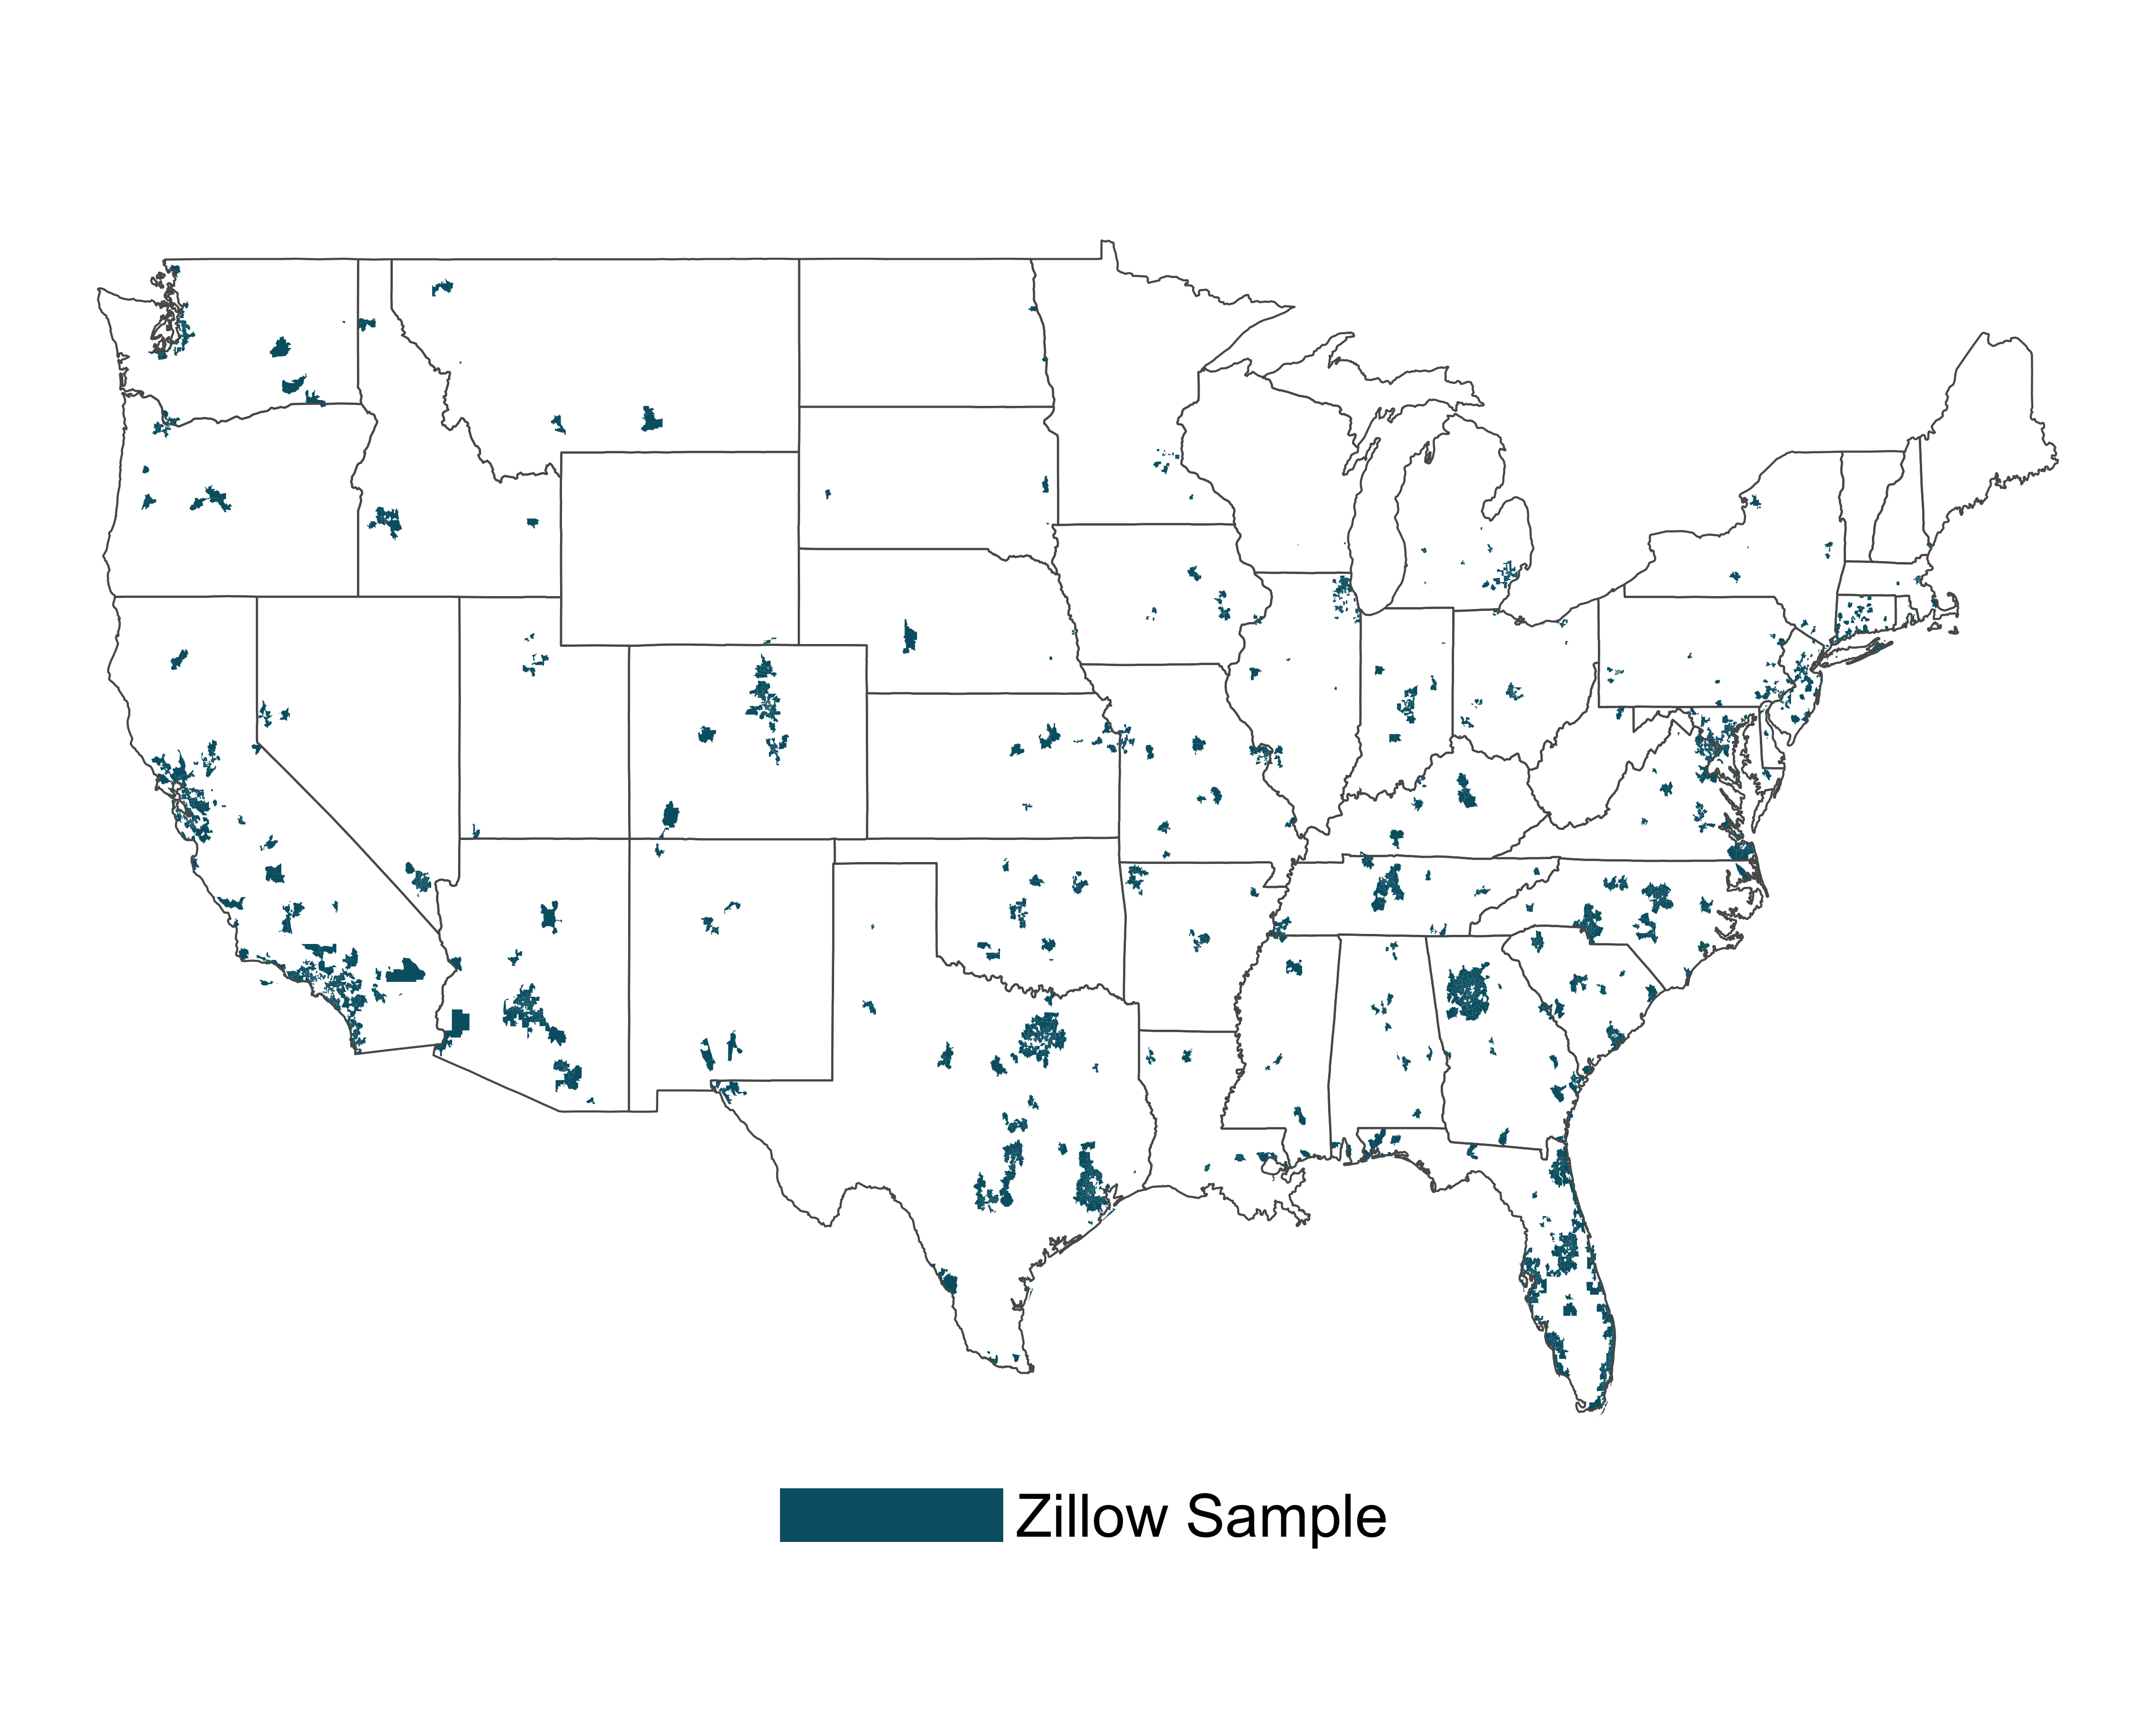
\includegraphics[width = .85\textwidth]{../../analysis/descriptive_maps/output/sample_map.png}
	\end{subfigure}
	\quad 
	\begin{subfigure}[b]{\textwidth}\centering
		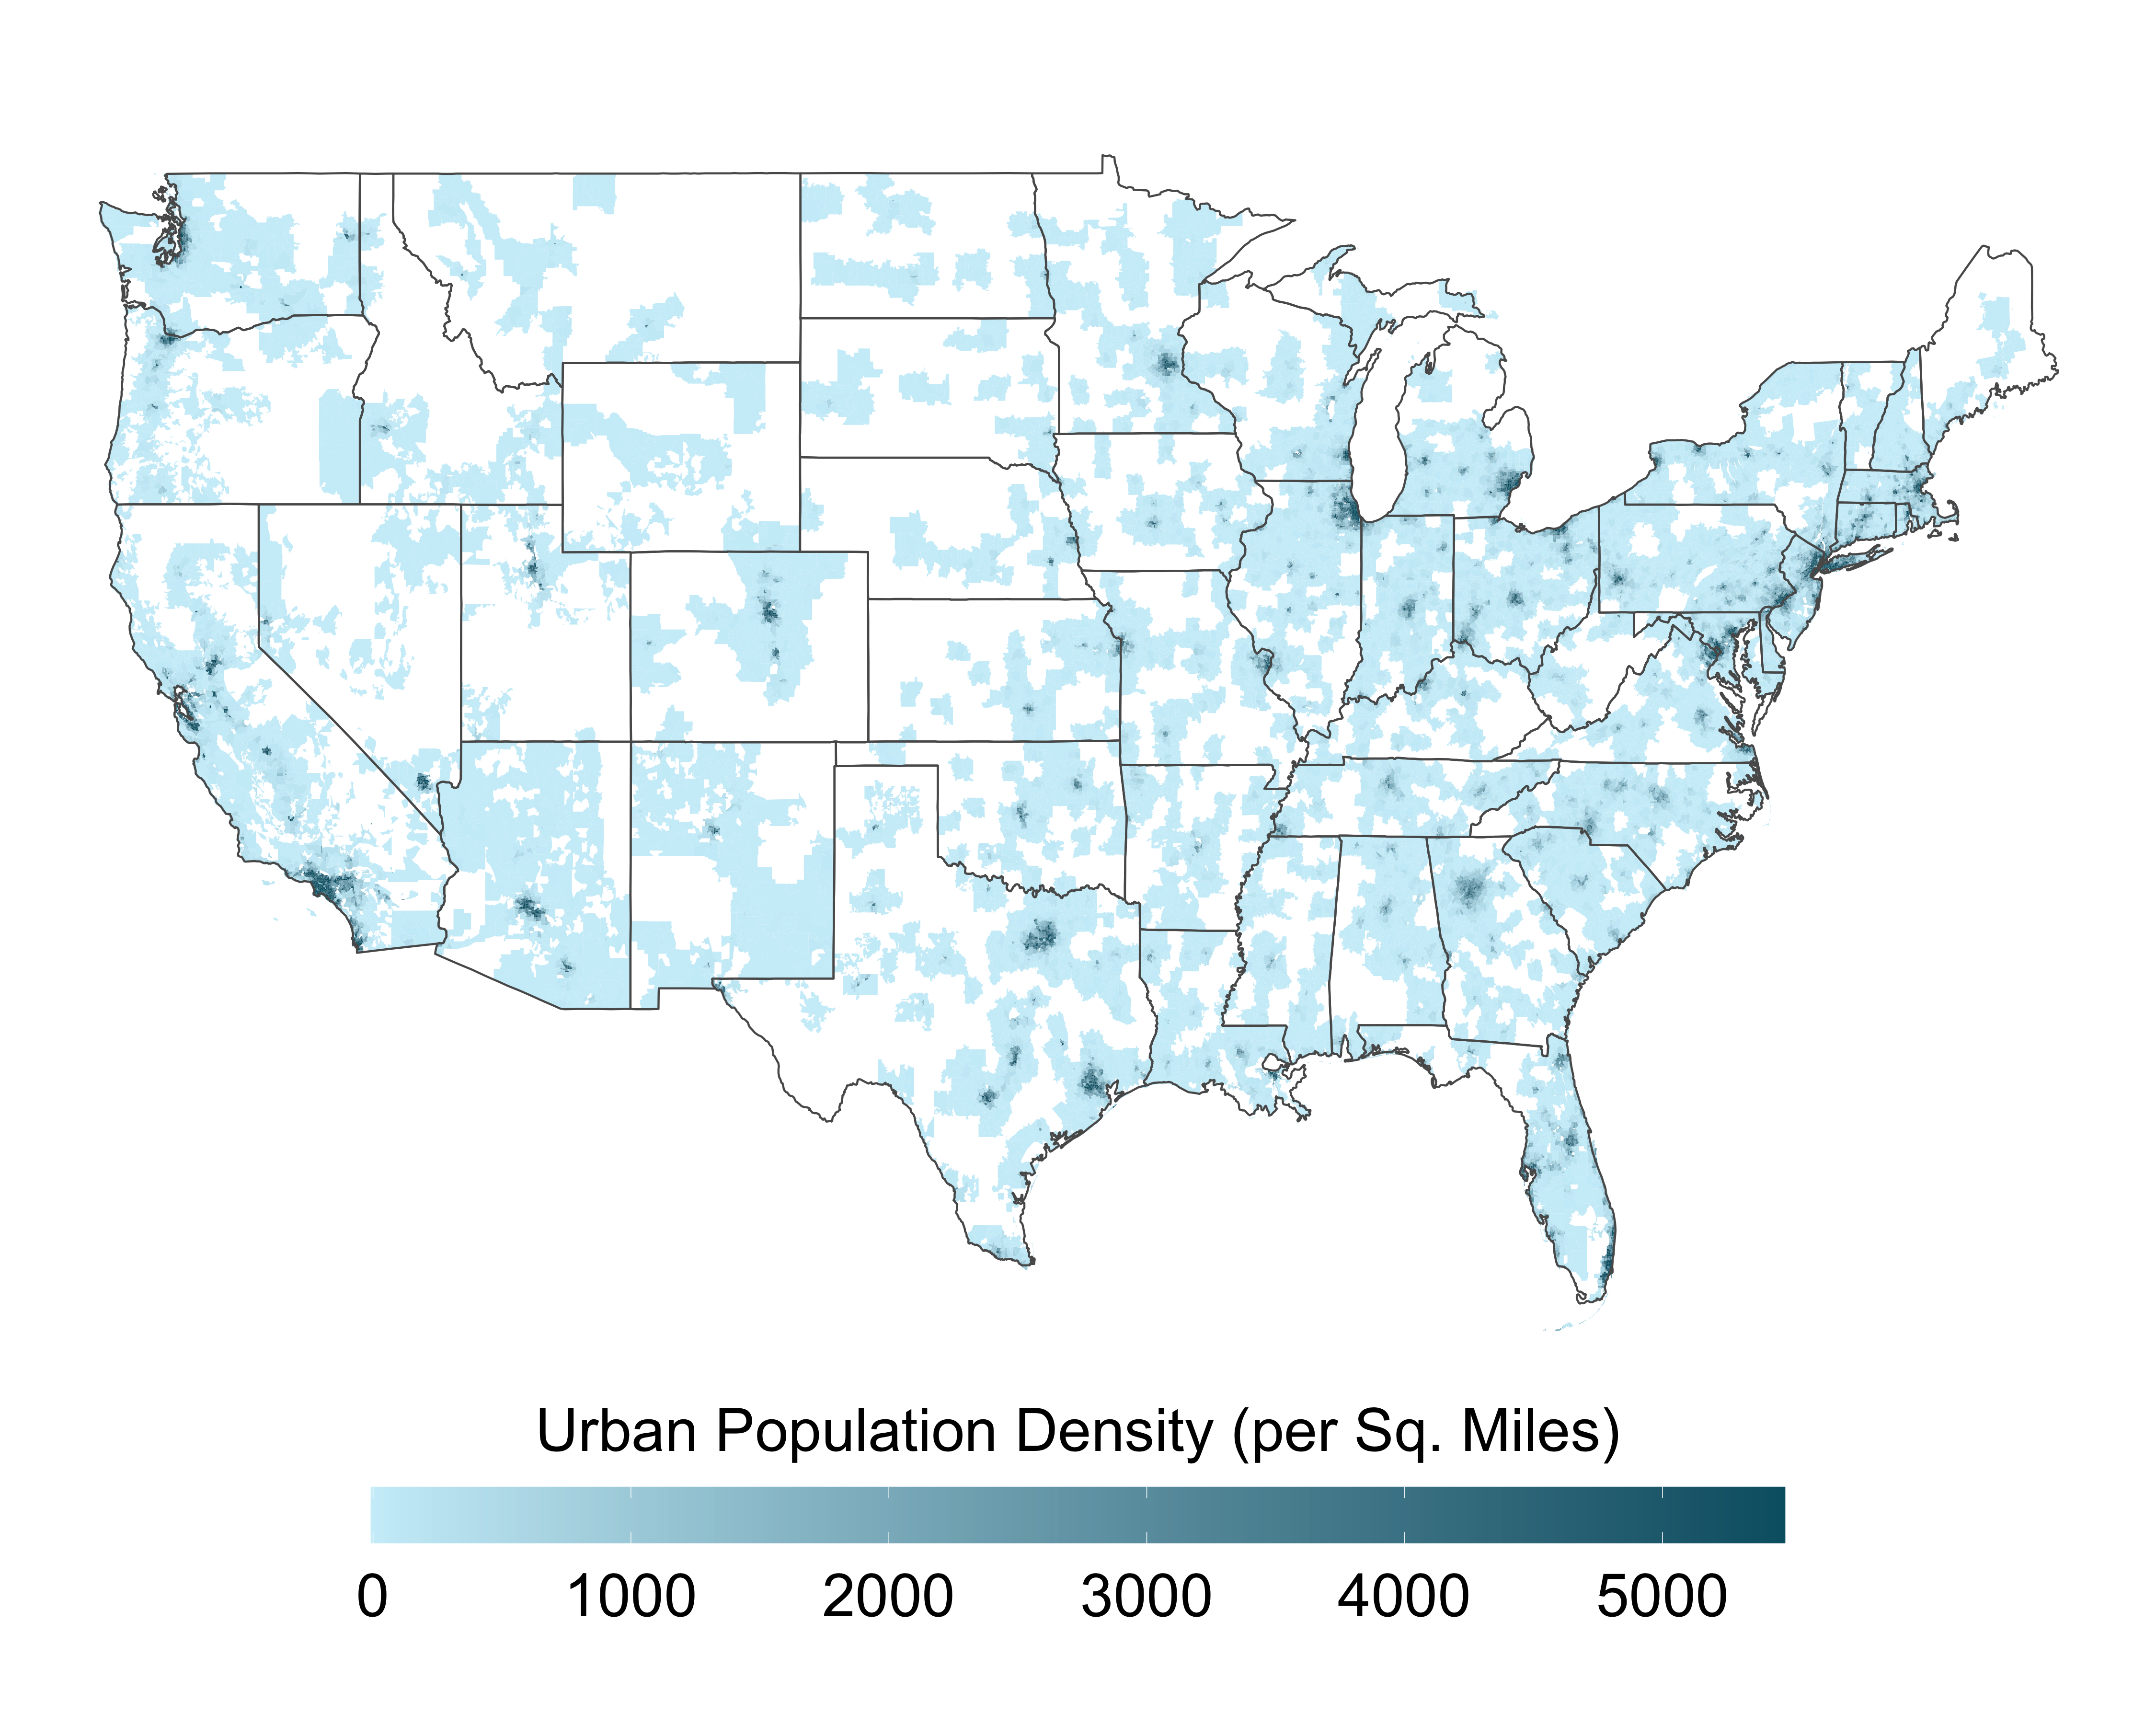
\includegraphics[width = .85\textwidth]{../../analysis/descriptive_maps/output/popurban_density_map.png}
	\end{subfigure}
		\begin{minipage}{.95\textwidth} \footnotesize
		\vspace{2mm} 
		\textit{Notes}: Panel (a) shows the geographical location of the ZIP codes present in the Zillow 
		SFCC sample used in the main analysis. Summary statistics for these units are reported in the main
		paper (\autoref{tab:desc_stats}, column 3). Panel (b) shows the urban population density for the top 
		100 metropolitan areas in the U.S. as reported in the 2008-2011 ACS. Values are winsorized at the 99 
		percentile to provide enough graphical variation.
	\end{minipage}
\end{figure}

\clearpage
\begin{figure}[!h]
	\caption{Coefficients of Dynamic Model for Different Sets of Controls}
	\label{fig:}
	\centering
	\includegraphics[width = 0.7\textwidth]
		{../../analysis/first_differences/output/fd_models_control.eps}
	\begin{minipage}{.95\textwidth} \footnotesize
		\vspace{2mm} 
		\textit{Notes}: The figure shows the estimated coefficients of the dynamic model defined 
		in equation \autoref{eq:leads_lags} when progressively adding time-varying economic controls 
		from the QCEW. The \textit{baseline} series plots coefficients taken from 
		\autoref{tab:dynamic_lags_leads_main}, column (1). The \textit{employment}, \textit{establishment}, 
		\textit{wage}, and \textit{all} results add employment controls, wage controls and establishment 
		count controls and all from the industries ``Professional and business services'', ``Information'', 
		and ``Financial activities''. These correspond to columns (2) to (5) in Appendix 
		\autoref{tab:dynamic_lags_leads_main}. 90 percent confidence intervals clustered at the state 
		level reported.
	\end{minipage}
\end{figure}

\clearpage
\begin{figure}[htb!]
	\caption{Dynamic coefficients for different window $s$}
	\label{fig:dynamic_change_window}
	\centering
	\begin{subfigure}[b]{0.5\textwidth}
		\caption{$s=3$}
		\includegraphics[width = .92\textwidth]
		{../../analysis/first_differences/output/fd_models_coeffs_w3.eps}
	\end{subfigure}\\
	\begin{subfigure}[b]{0.5\textwidth}
		\caption{$s=6$}
		\includegraphics[width = .985\textwidth]
		{../../analysis/first_differences/output/fd_models_coeffs_w6.eps}
	\end{subfigure}%
	\begin{subfigure}[b]{0.5\textwidth}
		\caption{$s=9$}
		\includegraphics[width = .985\textwidth]
		{../../analysis/first_differences/output/fd_models_coeffs_w9.eps}
	\end{subfigure}
	\begin{minipage}{0.95\textwidth} \footnotesize
		\vspace{2mm} 
		\textit{Notes}: The figure shows the estimated coefficients of the dynamic model defined 
		in equation \autoref{eq:leads_lags} for different values of the leads and lags window $s$.
		All models control for 	monthly date fixed effects. All models additionally include the
		following economic controls from the industries ``Professional and business services'', 
		``Information'', and ``Financial activities'' in the QCEW: the difference in the natural 
		logarithm of average weekly wages, the difference in the natural logarithm of employment, 
		and the difference in the natural logarithm of number of establishments. Wages and 
		employment vary at the county-month level, whereas establishment count varies at the 
		country-quarter level. Both panels	show 90 percent confidence intervals for the estimates, 
		clustered at the state level.
	\end{minipage}
\end{figure}

\begin{figure}[htb!]\centering
	\caption{Placebo Regression with Number of Listings for Sale}
	\label{fig:placebo_nlist}
	\includegraphics[width = 0.8\textwidth]
		{../../analysis/first_differences_nlist/output/fd_placebo.eps}	
	\begin{minipage}{0.95\textwidth}\footnotesize
		\textit{Notes:} The figure shows the estimated coefficients of the dynamic model defined 
		in equation \autoref{eq:leads_lags}. The dependent variable is the difference in the natural 
		logarithm of the number of listings \textit{for sale} in the Single Family, Condos, and 
		Cooperative category in Zillow. The model controls for monthly date fixed effects. In 
		addition, it includes the following economic controls from the industries ``Professional and 
		business services'', ``Information'', and ``Financial activities'' in the QCEW: the difference 
		in the natural logarithm of average weekly wages, the difference in the natural logarithm 
		of employment, and the difference in the natural logarithm of number of establishments. Wages 
		and employment vary at the county-month level, whereas establishment count varies at the 
		country-quarter level. 90 percent confidence intervals clustered at the state level reported. 
	\end{minipage}
\end{figure}

\begin{figure}[htb!]\centering
	\caption{Comparison between Dynamic Models on Baseline, Reweighted and Unbalanced Samples}
	\label{fig:dynamic_wgt_unabl_comp}
	\begin{subfigure}[b]{0.75\textwidth}
		\caption{Baseline-Re weighted Models}	
		\includegraphics[width = \textwidth]
			{../../analysis/first_differences_wgt/output/fd_model_comparison_wgt.eps}
	\end{subfigure}
	\quad
	\begin{subfigure}[b]{0.75\textwidth}
		\caption{Baseline-Unbalanced Models}		
		\includegraphics[width = \textwidth]
			{../../analysis/first_differences_unbal/output/fd_model_comparison_unbal.eps}
	\end{subfigure}
	\begin{minipage}{0.95\textwidth}\footnotesize
		\textit{Notes:} Panel (a) compares estimated coefficients of the dynamic model defined in 
		\autoref{eq:leads_lags} obtained from the baseline sample with those obtained from the 
		reweighted sample. Observations are weighted so as to match the average of the following 
		top-100 CBSA characteristics: ``share of rental houses", ``share of African-American 
		residents", ``share of college graduates", and ``median income". All characteristics are 
		obtained from the 2010 U.S. Census and the 2008-2011 ACS. See \autoref{sec:sample_rest} for 
		more details. Panel (b) compares estimated coefficients of the dynamic model defined in 
		\autoref{eq:leads_lags} obtained from the baseline sample with those obtained using the 
		unbalanced full sample of Zillow ZIP codes. The latter model controls for period of entry 
		$\times$ ZIP code fixed effects. Both panels additionally show, for each model, the 
		cumulative effect obtained by summing up estimates from a distributed lags only specification. 
		All models control for monthly date fixed effects. All models additionally include economic 
		controls from the industries ``Professional and business services'', ``Information'', and 
		``Financial activities'' from the QCEW. For each sector, we include the difference in the 
		natural logarithm of average weekly wages, the difference in the natural logarithm of 
		employment, and the difference in the natural logarithm of number of establishments. Wages 
		and employment vary at the county-month level, whereas establishment count varies at the 
		country-quarter level.
		90 percent confidence intervals clustered at the state level reported. 
	\end{minipage}
\end{figure}


\begin{figure}[h!]\centering
	\caption{Distribution of LODES-based ZIP code-level State Shares of Minimum Wage 
			Workers and Residents}
	\label{fig:lodes_share_dist}
	\begin{subfigure}[b]{0.75\textwidth}
	\caption{Share of MW Workers}	
	\includegraphics[width = \textwidth]
		{../../analysis/first_differences_expmw/output/walall_29y_lowinc_ssh_dist.eps}
	\end{subfigure}
	\quad
	\begin{subfigure}[b]{0.75\textwidth}
		\caption{Share of MW Residents}		
		\includegraphics[width = \textwidth]
			{../../analysis/first_differences_expmw/output/halall_29y_lowinc_ssh_dist.eps}
	\end{subfigure}
	\begin{minipage}{0.95\textwidth}\footnotesize
		\textit{Notes:} Panel (a) shows the distribution for the ZIP code-level state share of MW 
		\textit{workers} identified through the LODES data. Panel (b) shows the distribution of the 
		ZIP code-level state share of MW \textit{residents} identified through the LODES data. Both 
		shares are computed dividing the number of workers/residents 29 years old or younger earning 
		less than \$1,250 per month by state totals. For more details on the construction of the 
		shares, see \autoref{sec:mw_construction}.		
	\end{minipage}	
\end{figure}

\begin{figure}[htb!]\centering
	\caption{Static Effect of the Minimum Wage on Rents by Workplace and Residence of Young, 
			Low-income Workers}
	\label{fig:static_qtl_lodes}
	\begin{subfigure}[b]{.5\textwidth}
		\caption{State Share, Workplace}
		\includegraphics[width = \textwidth]
			{../../analysis/first_differences_expmw/output/fd_static_heter_walall_29y_lowinc_ssh_st_qtl.eps}
	\end{subfigure}%
	\begin{subfigure}[b]{.5\textwidth}
		\caption{State Share, Residence}
		\includegraphics[width = \textwidth]
			{../../analysis/first_differences_expmw/output/fd_static_heter_halall_29y_lowinc_ssh_st_qtl.eps}
	\end{subfigure}\\
	\begin{subfigure}[b]{.5\textwidth}
		\caption{ZIP code Share, Workplace}
		\includegraphics[width = \textwidth]
			{../../analysis/first_differences_expmw/output/fd_static_heter_walall_29y_lowinc_zsh_st_qtl.eps}
	\end{subfigure}%
	\begin{subfigure}[b]{.5\textwidth}
		\caption{ZIP code Share, Residence}
		\includegraphics[width = \textwidth]
			{../../analysis/first_differences_expmw/output/fd_static_heter_halall_29y_lowinc_zsh_st_qtl.eps}
	\end{subfigure}
	\begin{minipage}{0.95\textwidth}\footnotesize
		\vspace{3mm}	
		\textit{Notes:} The figure reports the estimated static effect of MW on rents for different 
		quartile groups across the distribution of young, low-income workers. More precisely, we estimate
		our static model interacting the MW variable with indicators for quartile groups of ZIP code-level 
		characteristics, as explained in \autoref{sec:strategy_heterogeneity}. All figures use counts of 
		workplace and residence of young, low-income workers constructed from LODES data. The top 
		row assigns to each ZIP code the share of young, low-income workers that work or live there out 
		of state totals. The bottom row constructs a ZIP code share of young, low-income workers out of 
		the working population of that ZIP code. All models control for monthly date fixed effects. All 
		models additionally include economic controls from the industries ``Professional and business 
		services'', ``Information'', and ``Financial activities'' from the QCEW, as specified throughout
		the paper. 90 percent confidence intervals clustered at the state level reported. 
	\end{minipage}
\end{figure}

\begin{figure}[htb!]\centering
	\caption{Residual Variation in the Experienced Minimum Wage and Different Types of Events}
	\label{fig:residu_expmw}
	\begin{subfigure}[b]{.7\textwidth}
		\caption{State Events}
		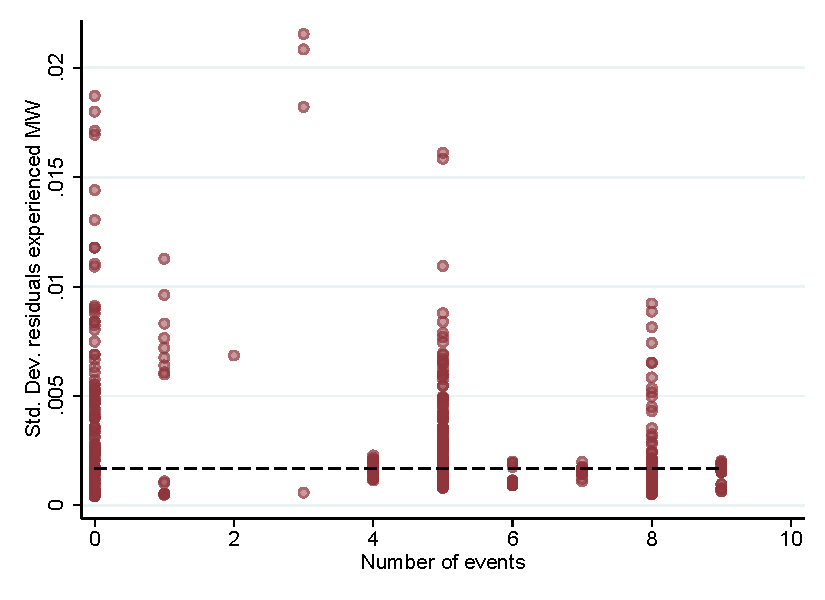
\includegraphics[width = \textwidth]
			{../../analysis/first_differences_expmw/output/resid_expmw_state_event.pdf}
	\end{subfigure}\\
	\begin{subfigure}[b]{.7\textwidth}
		\caption{Local Events}
		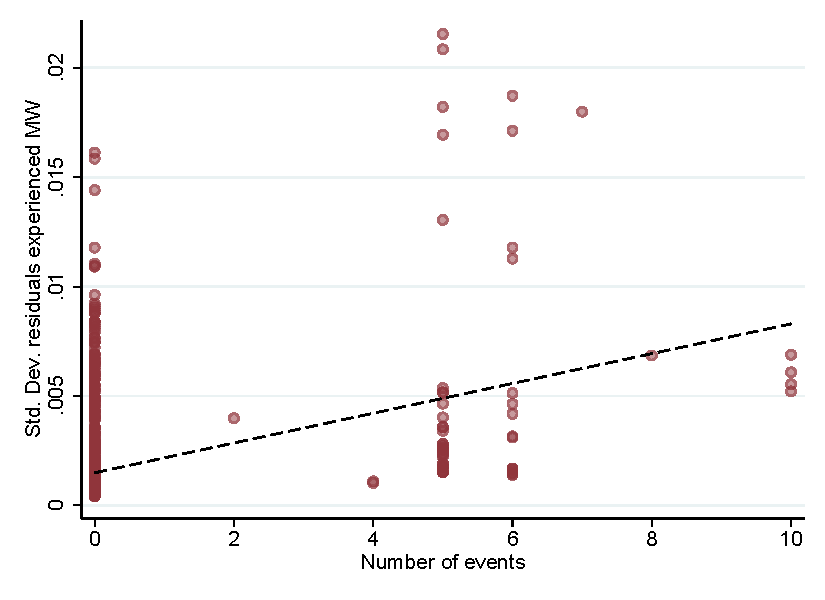
\includegraphics[width = \textwidth]
			{../../analysis/first_differences_expmw/output/resid_expmw_local_event.pdf}
	\end{subfigure}
	\begin{minipage}{0.95\textwidth}\footnotesize
		\vspace{3mm}	
		\textit{Notes:} The figures show a scatter plot of the residual variation in the 
		experienced MW versus the number of MW events of a certain type, where each dot represents 
		a ZIP code. The y-axis corresponds to the standard deviation of the residuals from the static 
		model using the difference in the natural logarithm of the experienced MW as dependent variable. 
		These regressions use the set of our preferred economic controls from the QCEW, and corresponds 
		to results reported in the first column of \autoref{tab:expmw_main} in the main paper. The 
		x-axis counts the number of MW events arising either from the state or local levels in the 
		given ZIP code. The dashed line shows the OLS fit between the variables.
	\end{minipage}
\end{figure}

\begin{figure}[!h]
	\centering
	\caption{Dynamic Effect Experienced MW Changes on Rents}
	\label{fig:expmw_dynamic}
	\includegraphics[width = .75\textwidth]
		{../../analysis/first_differences_expmw/output/fd_model_comparison_expmw.eps}
	\begin{minipage}{.95\textwidth}\footnotesize
		\textit{Notes:} The figure compares estimated coefficients of the dynamic model defined in 
		\autoref{eq:leads_lags} obtained from the baseline sample with those obtained when replacing 
		the statutory MW with the experienced MW as main explanatory variable. The plot additionally 
		shows, for each model, the cumulative effect obtained by summing up estimates from a 
		distributed lags only specification. All models control for monthly date fixed effects. 
		All models additionally include economic controls from the industries ``Professional and 
		business services'', ``Information'', and ``Financial activities'' from the QCEW. For each
		sector, we include the difference in the natural logarithm of average weekly wages, the 
		difference in the natural logarithm of employment, and the difference in the natural 
		logarithm of number of establishments as controls. Wages and employment vary at the 
		county-month level, whereas establishment count varies at the country-quarter level.
		90 percent confidence intervals clustered at the state level reported. 
	\end{minipage}
\end{figure}

\clearpage
%%%%%%%%%%%%%%%%%%%%%%%%%%%%%%%%%%%%%%%%%%%%%%%%%%%%%%%%%%%%%%%%%%%%%%%%%%%%%%%%%
\section{The Rationale for Selecting Economic Controls}\label{sec:app_econ_control}

Throughout the paper we use wages, employment, and establishment-count from the QCEW to control 
for the local business cycle. However, those variables may themselves be impacted directly by 
changes in the MW. As a result, incorporating those controls raises the concern of a ``bad 
control'' problem \parencite{AngristPischke2009}. In the scenario that the MW affects the 
controls used in the regression, this approach will not unveil the average treatment effect of 
the MW on rents even if the policy is known to be \textit{randomly assigned}. The reason is 
that conditioning on these variables opens a potential alternative channel through which the MW 
affects rents, introducing bias in our estimates.

To avoid the ``bad controls" problem, while at the same time include control variables that 
proxy for the local economic conditions, we select QCEW county-level time-series for the sectors 
that we think are unlikely to be affected by MW legislation: "Professional and Business Services", 
"Information", and "Finance". Our interpretation of the effects of the MW on rents as causal 
relies on the assumption that these controls are not influenced by the MW. In this appendix we 
provide evidence in favor of this assumption.

We start by noting that these sectors employ a rather small portion of MW labor. According to 
\textcite[][table 5]{MinWorkersReportBLS}, in 2019 such industries accounted for 3.5, 1, and 
1.2 percent of the total number of MW workers, respectively. These low percentages make direct
impacts unlikely. However, these sectors may be influenced by MW legislation indirectly. We 
test this possibility by using a version of the dynamic model to analyze whether MW affects 
either wages, employment, or establishment-count in these sectors. The presence of significant 
pre-treatment trends would suggest that these sectors react to MW, and cast doubt on the 
identification strategy discussed in the paper.

For each industry, we observe employment at the county and month levels, and average weekly 
wages and establishment-count at the county and quarter levels. As a result, estimation of the 
dynamic model defined at the zipcode and month level is not straightforward. To be able to 
estimate our model, we aggregate MW zipcode-month information at the county-month level by 
taking, for each period, the weighted average of MW levels in each zipcode associated with a 
given county, using the number of housing units as weights. We call this our MW variable 
$\underline{w}_{ct}$, where $(c, t)$ is a county and monthly date cell.\footnote{For counties 
	without city level ordinances this procedure would simply reflect the state- or 
	county-level 	MW. For places with a MW at the city level our MW variable corresponds to a 
	weighted average between places affected by the city MW and places not affected by it.}

Given that we observe employment with monthly frequency, we are able to estimate the following 
model:

\begin{equation} \label{eq:dynamic_econ_cont_month}
\Delta \ln y_{ct} = \delta_{t} 
+ \sum_{r=-s}^{s} \beta_r \Delta \ln \underline{w}_{c,t+r} 
+ \Delta \nu_{ct} ,
\end{equation}
where $y_{ct}$ is the outcome variable (employment) in county $c$ and month $t$, and $s$ defines 
the number of leads and lags in the model.

Because the QCEW provides average weekly wages and establishment-count at the county-quarter level, 
we estimate the model for these variables in quarterly averages of monthly observations. We compute 
quarterly average of QCEW measures as $\overline{\Delta y}_{cq} = \frac{1}{3} \Delta y_{cq}$. As for 
MW data, we define $\underline{w}_{cq}$ as the third month in each quarter $q$. We are then able to 
compute the quarterly average for MW changes, $\overline{\Delta \ln \underline{w}}_{cq} = \frac{1}{3} 
\Delta \ln \underline{w}_{cq}$. The estimating model then becomes

\begin{equation} \label{eq:dynamic_econ_cont_quarter}
\overline{\Delta \ln y}_{cq} = \overline{\delta}_q 
+ \sum_{r=\tau}^{\tau} \rho_r \overline{\Delta \ln \underline{w}}_{c,q+r}
+ \overline{\Delta \nu}_{ct} ,
\end{equation}
where $\tau$ defines the quarterly window. We interpret the $\rho_r$ coefficients in 
\autoref{eq:dynamic_econ_cont_quarter} as averages of the monthly coefficients $\beta_r$ in 
\autoref{eq:dynamic_econ_cont_month}. The reason is that the average change over a quarter is a 
linear combination of monthly changes.\footnote{To see this, let's define $q_1, q_2, q_3$ as the 
	first, second, and third months in a quarter $q$, respectively. Then, for any variable $x$,
	\begin{equation*}
	\begin{split}
	\frac{1}{3}\Delta x_{cq} 
	& = \frac{1}{3} \left( x_{cq} - x_{c,q-1} \right) 
	= \frac{1}{3} \left( x_{cq_3} - x_{c,q_3-1} \right) \\
	& = \frac{1}{3} \left( x_{cq_3} - x_{cq_2} 
	+ x_{cq_2} - x_{cq_1} + x_{cq_1} - x_{c,q_3-1} \right) \\ 
	& = \frac{1}{3} \left( \Delta x_{cq_3} + \Delta x_{cq_2}  + \Delta x_{cq_1} \right) .
	\end{split}
	\end{equation*}}

\autoref{fig:controls_models} shows the results of our estimation for the three industries 
selected as controls. Even though some of the coefficients are significant, we interpret the 
results as suggestive of a noisy zero effect. The most worrisome sector is ``Professional 
and Business Services'', which shows a significant same quarter coefficient of average weekly
wages, and a slight negative pre-trend in employment. While we decided to keep this sector as
control in our main models, we stress that our results are virtually identical when dropping it.

\begin{figure}[htb!]\centering
	\caption{Dynamic Models Using Economic Controls as Dependent Variable}
	\label{fig:controls_models}
	\begin{subfigure}[b]{.55\textwidth}
		\caption{Financial activities}
		\includegraphics[width = \textwidth]
			{../../analysis/first_differences_controls/output/fd_models_fin_w3.eps}
	\end{subfigure}\\
	\begin{subfigure}[b]{.55\textwidth}
		\caption{Professional and business services}
		\includegraphics[width = \textwidth]
			{../../analysis/first_differences_controls/output/fd_models_bizserv_w3.eps}
	\end{subfigure}\\
	\begin{subfigure}[b]{.55\textwidth}
		\caption{Information}
		\includegraphics[width = \textwidth]
			{../../analysis/first_differences_controls/output/fd_models_info_w3.eps}
	\end{subfigure}
	\begin{minipage}{0.95\textwidth}\footnotesize
		\vspace{3mm}	
		\textit{Notes:} The figures shows estimates of the dynamic model using economic variables 
		from the QCEW as dependent variable. All variables in the QCEW are defined at the county level.
		We aggregate our statutory MW variable at the county as explained in the text. For average weekly 
		wage and establishment count, provided by the QCEW with quarterly frequency, we regress the average 
		difference in that variable on the average difference in the natural logarithm of the MW, three 
		leads and lags of that	same variable, and time-period fixed effects. For employment, provided at a 
		monthly frequency, we regress its monthly difference on the monthly difference in (log) MW, nine 
		leads and lags, and time-period fixed effects. We report the coefficients on the MW variables in 
		each case, together with 90\% confidence bands. Standard errors are clustered at the state level.
	\end{minipage}
\end{figure}





\clearpage
%%%%%%%%%%%%%%%%%%%%%%%%%%%%%%%%%%%%%%%%%%%%%%%%%%%%%%%%%%%%%%%%%%%%%%%%%%%%%%%%
\section{Additional Tables and Figures}

\begin{table}[hbt!] \centering
    \caption{Summary statistics of baseline panel}
    \label{tab:stats_est_panel}
    \begin{tabular}{@{}lccccc@{}}
        \toprule
                                          & \multicolumn{1}{c}{N} 
                                          & \multicolumn{1}{c}{Mean} 
                                          & \multicolumn{1}{c}{St. Dev.} 
                                          & \multicolumn{1}{c}{Min} 
                                          & \multicolumn{1}{c}{Max}                 \\ \midrule
        \textit{Minimum wage variables:}              &       &       &       &       &       \\
        $\quad$Statutory MW $\MW_{it}$                & 133,600  & 8.20  & 1.34  & 7.25  & 16.00  \\
        $\quad$Residence MW $\mw^{\res}_{it}$         & 133,600  & 2.092  & 0.144  & 1.981  & 2.773  \\
        $\quad$Workplace MW $\mw^{\wkp}_{it}$         & 133,600  & 2.095  & 0.141  & 1.981  & 2.694  \\
        $\quad$Workplace MW, low-income workers       & 133,600  & 2.094  & 0.139  & 1.981  & 2.681  \\
        $\quad$Workplace MW, young workers            & 133,600  & 2.094  & 0.140  & 1.981  & 2.707  \\[.3em]
        \textit{Median Rents:}                        &       &       &       &       &       \\
        $\quad$SFCC                                   & 114,525  & 1,658.78  & 822.41  & 595.00  & 30,000.00  \\
        $\quad$SFCC per sqft.                         & 133,600  & 1.23  & 0.90  & 0.42  & 22.20  \\
        $\quad$Log(SFCC per sqft.)                    & 133,600  & 0.08  & 0.46  & -0.87  & 3.10  \\
        $\quad$Log(single family (SF) per sqft.)      & 99,783  & -0.04  & 0.37  & -0.87  & 3.10  \\
        $\quad$Log(condo/cooperatives (CC) per sqft.) & 24,735  & 0.63  & 0.47  & -0.54  & 1.92  \\
        $\quad$Log(Studio per sqft.)                  & 14,545  & 0.31  & 0.75  & -0.85  & 1.97  \\
        $\quad$Log(1 Bedroom per sqft.)               & 25,947  & 0.73  & 0.40  & -0.31  & 1.90  \\
        $\quad$Log(2 Bedroom per sqft.)               & 43,770  & 0.43  & 0.43  & -0.69  & 1.87  \\
        $\quad$Log(3 Bedroom per sqft.)               & 48,672  & 0.05  & 0.39  & -0.68  & 1.87  \\
        $\quad$Log(multifamily 5+ units per sqft.)    & 55,640  & 0.44  & 0.44  & -0.67  & 1.90  \\[.3em]
        \textit{Economic controls:}                   &       &       &       &       &       \\
        $\quad$Avg.\ wage Business services           & 133,600  & 11.15  & 1.36  & 5.80  & 13.39  \\
        $\quad$Employment Business services           & 133,600  & 8.69  & 1.24  & 4.13  & 10.96  \\
        $\quad$Estab. count Business services         & 133,600  & 7.09  & 0.31  & 5.42  & 8.43  \\
        $\quad$Avg.\ wage Financial services          & 132,909  & 9.00  & 1.53  & 2.40  & 12.39  \\
        $\quad$Employment Financial services          & 133,600  & 6.11  & 1.33  & 1.39  & 9.53  \\
        $\quad$Estab. count Financial services        & 132,909  & 7.27  & 0.34  & 5.89  & 8.91  \\
        $\quad$Avg.\ wage Information services        & 133,576  & 10.20  & 1.42  & 4.75  & 12.90  \\
        $\quad$Employment Information services        & 133,600  & 7.98  & 1.20  & 3.50  & 10.34  \\
        $\quad$Estab. count Information services      & 133,576  & 7.25  & 0.37  & 6.22  & 9.16  \\ \bottomrule
    \end{tabular}

    \begin{minipage}{.95\textwidth} \footnotesize
        \vspace{2mm}
        Notes: This table shows summary statistics of the panel of ZIP codes 
        used in our baseline results, constructed as explained in Section 
        \ref{sec:data_final_panel}.
        All workplace MW variables use 2017 commuting data from LODES.
        The workplace MW variables ``Workplace MW, low-income workers'' and 
        ``Workplace MW, young workers'' are constructed using data for 
        workers who earn less \$1,251 and aged less than 29, respectively.
        We exclude rental categories with less than 10,000 non-missing ZIP code 
        by month observations.
        Excluded categories are ``4 Bedroom,'' ``5 bedroom,'' and 
        ``Duplex and triplex.''
    \end{minipage}
\end{table}

\clearpage
\begin{table}[hbt!] \centering
	\caption{Autocorrelation}
	\label{tab:autocorrelation}
    \begin{tabular}{@{}lcc@{}}
		\toprule
        & \multicolumn{2}{c}{Log rents}                                 \\ \cmidrule(l){2-3} 
        & \shortstack{Level}           & \shortstack{First Difference}  \\ \midrule
		                                   &  (1)   &  (2)              \\ \midrule
		Residence minimum wage             &  0.0862   &  -0.0204              \\
		                                   & (0.2144)  & (0.0169)             \\
		Workplace minimum wage             &  -0.0660   &  0.0545              \\
		                                   & (0.2159)  & (0.0283)             \\ \midrule
		County-quarter economic controls   &  Yes   &  Yes              \\
		P-value autocorrelation test       &        &  0.0000              \\
		Observations                       &  132,897  &  131,383             \\\bottomrule
	\end{tabular}

    \begin{minipage}{.95\textwidth} \footnotesize
        \vspace{2mm}
        \textit{Notes}: In column (1) we report results from a regression of log median SFCC rents 
        on residence and workplace MW levels with ZIP code and year-month fixed effects. 
        In column (2), we report the same regression but in first differences (note that the ZIP code 
        fixed effects drop out). For the model in first differences, we also report an AR 1 auto-correlation 
        test. We proceed as in \parencite[][section 10.6.3]{wooldridge2010}. We compute the residuals of 
        the model estimated in column (2), and we regress those residuals on their lag. We call that 
        coefficient $\rho$. The model in levels is efficient assuming no auto-correlation of the 
        error term, which would imply that the residuals of the first difference model are 
        auto-correlated with $\rho = -0.5$. We report the p-value of testing that hypothesis.
    \end{minipage}
\end{table}

\clearpage
\begin{table}[hbt!] \centering
    \caption{Estimates of the effect of the MW on rents, stacked sample}
    \label{tab:stacked_w6}
    \begin{tabular}{l*{4}{c}}
        \toprule
        & \multicolumn{1}{c}{\shortstack{Change wkp.\ MW\\$\Delta\mw_{it}^{\wkp}$}}
            & \multicolumn{3}{c}{\shortstack{Change log rents\\$\Delta r_{it}$}} \\ \cmidrule(lr){2-2}\cmidrule(lr){3-5}
                                            & (1)   & (2)   & (3)   & (4)            \\ \midrule
        Change residence MW 
                    $\Delta\mw_{it}^{\res}$  &  0.5461  &  0.0051  &       &  -0.0444     \\
                                            & (0.0316) & (0.0109) &       & (0.0174)    \\
        Change workplace MW 
                    $\Delta\mw_{it}^{\wkp}$ &       &       &  0.0242  & 0.0906      \\
                                            &       &       & (0.0216) & (0.0391)    \\ \midrule
        Sum of coefficients                &       &       &       &  0.0463     \\
                                            &       &       &       & (0.0266)    \\ \midrule
        County-quarter economic controls   &  Yes  & Yes   & Yes   & Yes      \\
        P-value equality                   &       &       &       & 0.0208      \\
        R-squared                          &  0.9763  &  0.0539  &  0.0540  & 0.0540      \\
        Observations                       & 98,326  & 98,326  & 98,326  & 98,326     \\\bottomrule
    \end{tabular}

    \begin{minipage}{.95\textwidth} \footnotesize
        \vspace{2mm}
        Notes: 
        Data are from Zillow \parencite{ZillowData}, 
        the minimum wage panel described in Section \ref{sec:data_mw_panel}, 
        LODES origin-destination statistics \parencite{CensusLODES},
        and the QCEW \parencite{QCEW}.
        The table mimics the estimates in Table \ref{tab:static} using a 
        ``stacked'' sample.
        To construct the sample we proceed as follows.
        First, we define a CBSA-month as treated if in that month there is at 
        least one ZIP code that had a change in the binding MW.
        We drop events that have less than 10 ZIP codes.
        For each of the selected CBSA-months we assign a unique event ID. 
        Second, for each event we take a window $w = 6$, and we keep all months 
        within that window for the ZIP codes that belong to the treated CBSA.
        If a ZIP code has missing data for some month within the window, we drop 
        the entire ZIP code from the respective event.
        For each column, we estimate the same regression as the analogous column 
        in Table \ref{tab:static} but include event indicators $\times$ year-month
        fixed effects.
    \end{minipage}
\end{table}

\clearpage
\begin{table}
    \caption{Static model with lagged dependent variable}
    \label{tab:static_ab}

    \begin{tabular}{@{}lcc@{}}
        \toprule
                               & \multicolumn{2}{c}{Change log rents}                       \\ \cmidrule(l){2-3}
                               & \shortsack{Baseline\\(1)} & \shortsack{Arellano-Bond\\(2)} \\ \midrule
        Change residence minimum wage     &  -0.0302           &  -0.0324                           \\
                                          & (-0.0302)          & (-0.0324)                          \\
        Change workplace minimum wage     &  0.0169           & 0.0205                            \\
                                          & (0.0169)          & (0.0205)                          \\
        Lagged change log rents           &                & 0.0645                            \\
                                          &                & (0.0689)                          \\ \midrule
        County-quarter economic controls  & Yes            & Yes                            \\
        P-value equality                  & 0.0645            & 0.0689                            \\
        R-squared                         & 0.0274            & 0.0356                            \\
        Observations                      & 0           & 0                           \\ \bottomrule
    \end{tabular}

    \begin{minipage}{.95\textwidth} \footnotesize
        \vspace{2mm}
        Notes: 
    \end{minipage}
\end{table}

\clearpage
\begin{landscape}
\begin{table}[ht!]
    \centering
    \caption{Comparison of estimates of the effect of the MW on rents, different
             Zillow categories}
    \label{tab:zillow_categories}
        
    \begin{tabular}{@{}lccccc@{}}
        \toprule
                                             & \multicolumn{1}{c}{\shortstack{Change wkp.\ MW\\$\Delta\mw_{it}^{\wkp}$}} 
                                             & \multicolumn{3}{c}{\shortstack{Change log rents\\$\Delta r_{it}$}}
                                             &                                                                         \\ \cmidrule(lr){2-2}\cmidrule(lr){3-5}
                                                 & \multicolumn{1}{c}{\shortstack{Change res.\ MW\\$\Delta\mw_{it}^{\res}$}}
                                                 & \multicolumn{1}{c}{\shortstack{Change res.\ MW\\$\Delta\mw_{it}^{\res}$}} 
                                                 & \multicolumn{1}{c}{\shortstack{Change wkp.\ MW\\$\Delta\mw_{it}^{\wkp}$}} 
                                                 & \shortstack{Sum of\\coefficients} 
                                                 & N                                    \\ \midrule
        $\quad$(a) Baseline (SFCC)               &  0.8705  &  -0.0207  &  0.0546  &  0.0339  & 131,383 \\
                                                 & (0.0298) & (0.0171) & (0.0281) & (0.0153) &      \\
        $\quad$(b) Single family (SF)            &  0.8820  &  0.0101  &  0.0299  &  0.0400  & 97,808 \\
                                                 & (0.0356) & (0.0469) & (0.0527) & (0.0127) &      \\
        $\quad$(c) Condo/Cooperatives (CC)       &  0.8018  &  -0.0317  &  0.0951  &  0.0634  & 24,315 \\
                                                 & (0.0421) & (0.0272) & (0.0524) & (0.0281) &      \\
        $\quad$(d) Studio                        &  0.8342  &  -0.0503  &  0.0455  &  -0.0048  & 14,290 \\
                                                 & (0.0443) & (0.0443) & (0.0553) & (0.0257) &      \\
        $\quad$(d) 1 Bedroom                     &  0.7835  &  0.0289  &  -0.0419  &  -0.0130  & 25,277 \\
                                                 & (0.0459) & (0.0257) & (0.0446) & (0.0219) &      \\
        $\quad$(e) 2 Bedroom                     &  0.8100  &  -0.0123  &  0.0040  &  -0.0083  & 42,732 \\
                                                 & (0.0330) & (0.0400) & (0.0502) & (0.0182) &      \\
        $\quad$(f) 3 Bedroom                     &  0.7998  &  -0.0932  &  0.1366  &  0.0434  & 47,426 \\
                                                 & (0.0487) & (0.0407) & (0.0658) & (0.0385) &      \\
        $\quad$(g) Multifamily 5+ units          &  0.8294  &  0.0027  &  0.0069  &  0.0096  & 54,520 \\
                                                 & (0.0313) & (0.0253) & (0.0370) & (0.0170) &      \\ \bottomrule
    \end{tabular}

    \begin{minipage}{.95\linewidth} \footnotesize
        \vspace{2mm}
        Notes:
        Data are from the baseline estimation sample described in Section 
        \ref{sec:data_final_panel}.
        Each row of the table shows two estimations on the same sample of ZIP 
        codes and months.
        The first column shows the results of a regression of the change in the 
        workplace MW measure on the change in the residence MW measure.
        The second through fourth columns show the results of a regression of 
        the change in log rents on the change in the residence MW and the 
        workplace MW, with the fifth column showing the sum of the coefficients 
        on the MW measures.
        All rent variables correspond to the median per square foot rent in a 
        Zillow category.
        All estimated regressions include fixed effects for each year-month and 
        economic controls at the county $\times$ quarter level from the QCEW.
        Row (a) repeats the results of Table \ref{tab:static}, using the 
        Single Family, Condominium and Cooperative Houses category.
        Rows (b) through (g) estimate the same regression using an analogous 
        rent variable for different Zillow categories.
        Excluded categories are ``4 Bedroom'', ``5 bedroom'', and 
        ``Duplex and triplex''.
        Standard errors in parentheses are clustered at the state level.
    \end{minipage}
\end{table}
\end{landscape}

\clearpage
\begin{landscape}
\begin{table}[ht!]
    \centering
    \caption{Comparison of estimates of the effect of the MW on rents across 
             geographies and time frames}
    \label{tab:static_geos_times}
    
    \begin{tabular}{@{}lccccc@{}}
        \toprule
                                                         & \multicolumn{1}{c}{\shortstack{Change workplace\\MW $\Delta\mw_{it}^{\wkp}$}} 
                                                         & \multicolumn{3}{c}{\shortstack{Change log rents\\$\Delta r_{it}$}}
                                                         &                                                                         \\ \cmidrule(lr){2-2}\cmidrule(lr){3-5}
                                                             & \multicolumn{1}{c}{\shortstack{Change residence\\MW $\Delta\mw_{it}^{\res}$}}
                                                             & \multicolumn{1}{c}{\shortstack{Change residence\\MW $\Delta\mw_{it}^{\res}$}}
                                                             & \multicolumn{1}{c}{\shortstack{Change workplace\\MW $\Delta\mw_{it}^{\wkp}$}} 
                                                             & \shortstack{Sum of\\coefficients}
                                                             & N                                                                    \\ \midrule
        \textit{Panel A: Baseline (ZIP code $\times$ Month)}          &       &       &       &       &      \\
        $\quad$(i) Residence MW only                         &       &  0.0393  &       &       & 78,912 \\
                                                             &       & (0.0150) &       &       &      \\
        $\quad$(ii) Workplace MW only                        &       &       &  0.0473  &       & 78,912 \\
                                                             &       &       & (0.0161) &       &      \\
        $\quad$(iii) Both residence and workplace MW         &  0.8617  &  -0.0199  &  0.0687  &  0.0488  & 78,912 \\
                                                             & (0.0382) & (0.0195) & (0.0298) & (0.0162) &      \\
        \textit{Panel B: County $\times$ Month}              &       &       &       &       &      \\
        $\quad$(i) Residence MW only                         &       &  0.0057  &       &       & 27,267 \\
                                                             &       & (0.0188) &       &       &      \\
        $\quad$(ii) Workplace MW only                        &       &       &  0.0102  &       & 27,267 \\
                                                             &       &       & (0.0219) &       &      \\
        $\quad$(iii) Both residence and workplace MW         &  0.8768  &  -0.0509  &  0.0646  &  0.0137  & 27,267 \\
                                                             & (0.0199) & (0.0387) & (0.0506) & (0.0227) &      \\
        \textit{Panel C: ZIP code $\times$ Year}             &       &       &       &       &      \\
        $\quad$(i) Residence MW only                         &       &  0.0072  &       &       & 6,696 \\
                                                             &       & (0.0637) &       &       &      \\
        $\quad$(ii) Workplace MW only                        &       &       &  0.0092  &       & 6,696 \\
                                                             &       &       & (0.0701) &       &      \\
        $\quad$(iii) Both residence and workplace MW         &  0.8993  &  -0.0205  &  0.0308  &  0.0103  & 6,696 \\
                                                             & (0.0263) & (0.0891) & (0.1139) & (0.0698) &      \\ \bottomrule
    \end{tabular}
    
    \begin{minipage}{.95\linewidth} \footnotesize
        \vspace{2mm}
        Notes:
        Data are from the baseline estimation samples described in Section 
        \ref{sec:data_final_panel}.
        The first column and rows labeled (iii) show the results of a regression 
        of the change in the workplace MW measure on the change in the 
        residence MW measure.
        The second through fourth columns show the results of regressions of the 
        change in log rents on either the change in the residence MW---rows (i)---
        or the workplace MW---rows (ii)--- 
        or both---rows (iii)---, with the fifth column showing the sum of the 
        coefficients on the MW measures.
        The last column shows the number of observations, fixed within each row.
        All regressions include economic controls from the QCEW, as defined in
        Table \ref{tab:static}.
        Regressions estimated at a yearly frequency use the yearly average of
        the change in the MW measures and the change in the economic controls.
        Panel A repeats our baseline results from Table \ref{tab:static}, where 
        the unit of observation is the ZIP code $\times$ month.
        Panel B shows results for a panel where the unit of observation is the 
        county $\times$ month.
        Panel C shows results for a panel where the unit of observation is the 
        ZIP code $\times$ year.
        In all panels,
        (i) displays the results of a regression of the change in log rents on 
        the residence MW only;
        (ii) displays the results of a regression of the change in log 
        rents on the workplace MW only; and
        (iii) displays the results of a regression of the change in workplace
        MW on the change in residence MW (column 1), and of the change in 
        log rents on both MW measures (columns 2--5).
        Standard errors in parentheses are clustered at the state level.
    \end{minipage}
\end{table}
\end{landscape}

\clearpage
\begin{table}[hbt!]
    \centering
    \caption{Estimates of the effect of the minimum wage on income, full sample}
    \label{tab:static_wages}

    \begin{tabular}{@{}lccccc@{}}
        \toprule
                                & \multicolumn{4}{c}{Log wage income}
                                & \multicolumn{1}{c}{Log div.}                             \\ \cmidrule(lr){2-5}\cmidrule(lr){6-6}
                                & (1)       & (2)      & (3)      & (4)       & (5)        \\ \midrule
        Wkp.\ MW            & #4#       & #4#      & #4#      & #4#       & #4#        \\
                                & (#4#)     & (#4#)    & (#4#)    & (#4#)     & (#4#)      \\
        Wkp.\ MW $\times$ Std.\ 
            sh.\ of MW workers &           &          &          & #4#       &            \\
                                &           &          &          & (#4#)     &            \\ \midrule
        Economic controls       & No        & Yes      & Yes      & Yes       & Yes        \\
        CBSA $\times$ year FE   & No        & No       & Yes      & Yes       & Yes        \\
        Within R-squared        & #4#       & #4#      & #4#      & #4#       & #4#        \\
        Observations            & #0,#      & #0,#     & #0,#     & #0,#      & #0,#       \\ \bottomrule
    \end{tabular}

    \begin{minipage}{.95\textwidth} \footnotesize
        \vspace{2mm}
        Notes: 
        Income data are from the IRS, commuting data are from LODES, and MW
        data are from the panel described in Section \ref{sec:data_mw_panel}.
        The table shows different estimations of the effect of the workplace MW
        on income measures using a regression model that includes ZIP code and 
        year fixed effects.
        The sample includes all ZIP codes with valid income data for the years 
        2014--2019.
        The workplace MW and the economic controls are defined as the yearly 
        average of the respective variables used in our baseline estimates of 
        Section \ref{sec:results_main}.
        Columns (1) through (3) show estimates of a regression of log total wage
        income on the workplace MW and ZIP code and year fixed effects.
        Column (2) adds time-varying economic controls from the QCEW.
        Column (3) interacts the year fixed effects with indicators for each
        Core-Based Statistical Area (CBSA).
        Column (4) interacts the workplace MW with the standardized share of MW 
        workers (``Std.\ sh.\ of MW workers'') discussed in Section 
        \ref{sec:data_income_housing}.
        Column (5) repeats the estimation in column (3) but using the log of 
        total dividends (``Log div.'') as dependent variable.
        Standard errors in parentheses are clustered at the state level.
    \end{minipage}
\end{table}


\clearpage
\begin{table}[hbt!]
    \centering
    \caption{Effect of an increase in federal MW to \$7.97 and to \$15 in January 2020, 
             urban ZIP codes}
    \label{tab:counterfactuals_other}

    \begin{tabular}{@{}lccccc@{}}
        \toprule
                            &   & \multicolumn{2}{c}{Average change in...}
                                & \multicolumn{2}{c}{Avg.\ share pocketed}             \\ \cmidrule(lr){3-4} \cmidrule(l){5-6}
                            & N & Res.\ MW & Wkp.\ MW
                            & $s = $ 0.25  & $s = $ 0.45                                 \\ \midrule
        \textit{Panel A: Fed.\ MW to \$7.97}         &      &       &       &     &      \\
        $\quad $Effect in ZIP codes with...          &      &       &       &     &      \\
        $\quad \quad$previous MW $\leq\$7.97\quad$   & 3,751 &  0.095 & 0.090  & 0.074 &  0.134   \\
        $\quad \quad$previous MW $>\$7.97\quad$      & 1,235 &  0 & 0.008  & 0.126 & 0.227    \\[.3em]
        \textit{Panel B: Fed.\ MW to \$15}          &      &       &       &     &      \\
        $\quad $Effect in ZIP codes with...          &      &       &       &     &      \\
        $\quad \quad$previous MW $\leq\$15\quad$     & 10,994 &  0.494 & 0.480  & 0.075 &  0.135   \\
        $\quad \quad$previous MW $>\$15\quad$        & 260 &  0 & 0.054  & 0.126 & 0.226    \\ \bottomrule
    \end{tabular}
    
    \begin{minipage}{.95\textwidth} \footnotesize
        \vspace{2mm}
        Notes: 
        Data are from LODES and the minimum wage panel described in Section 
        \ref{sec:mw_construction}.
        The table shows averages of the estimated ZIP-code specific shares of the 
        additional income pocketed by landlords (``share pocketed''),
        defined as the ratio of the increase in income to the increase in rents.
        Increases in income and rents are simulated following the procedure
        described in Section \ref{sec:counterfactual}. 
        Panel A assumes a 10\% increase in the federal MW, and
        Panel B assumes an increase in the federal MW to \$15.
        We assume the following parameter values:
        $\beta = 0.0546$, $\gamma = -0.0207$, $\varepsilon = 0.1083$, and 
        $s\in\{0.25, 0.45\}$.
        We carry out our computations only for urban ZIP codes, defined as 
        those that belong to a CBSA with at least 80\% of urban population
        according to the 2010 census.
        The figure excludes ZIP codes located in CBAs for which the average
        estimated change in log total wages was below 0.1\% in the respective
        counterfactual scenario.
    \end{minipage}
\end{table}

\clearpage
\begin{figure}[h!]
    \centering
    \caption{Changes in Chicago-Naperville-Elgin CBSA due to a counterfactual raise 
    	     of the federal MW to \$9 in January 2020}
    \label{fig:map_chicago_cf_wkp_res}
    
    \begin{subfigure}{.49\textwidth}
        \caption*{Changes in residence MW}
        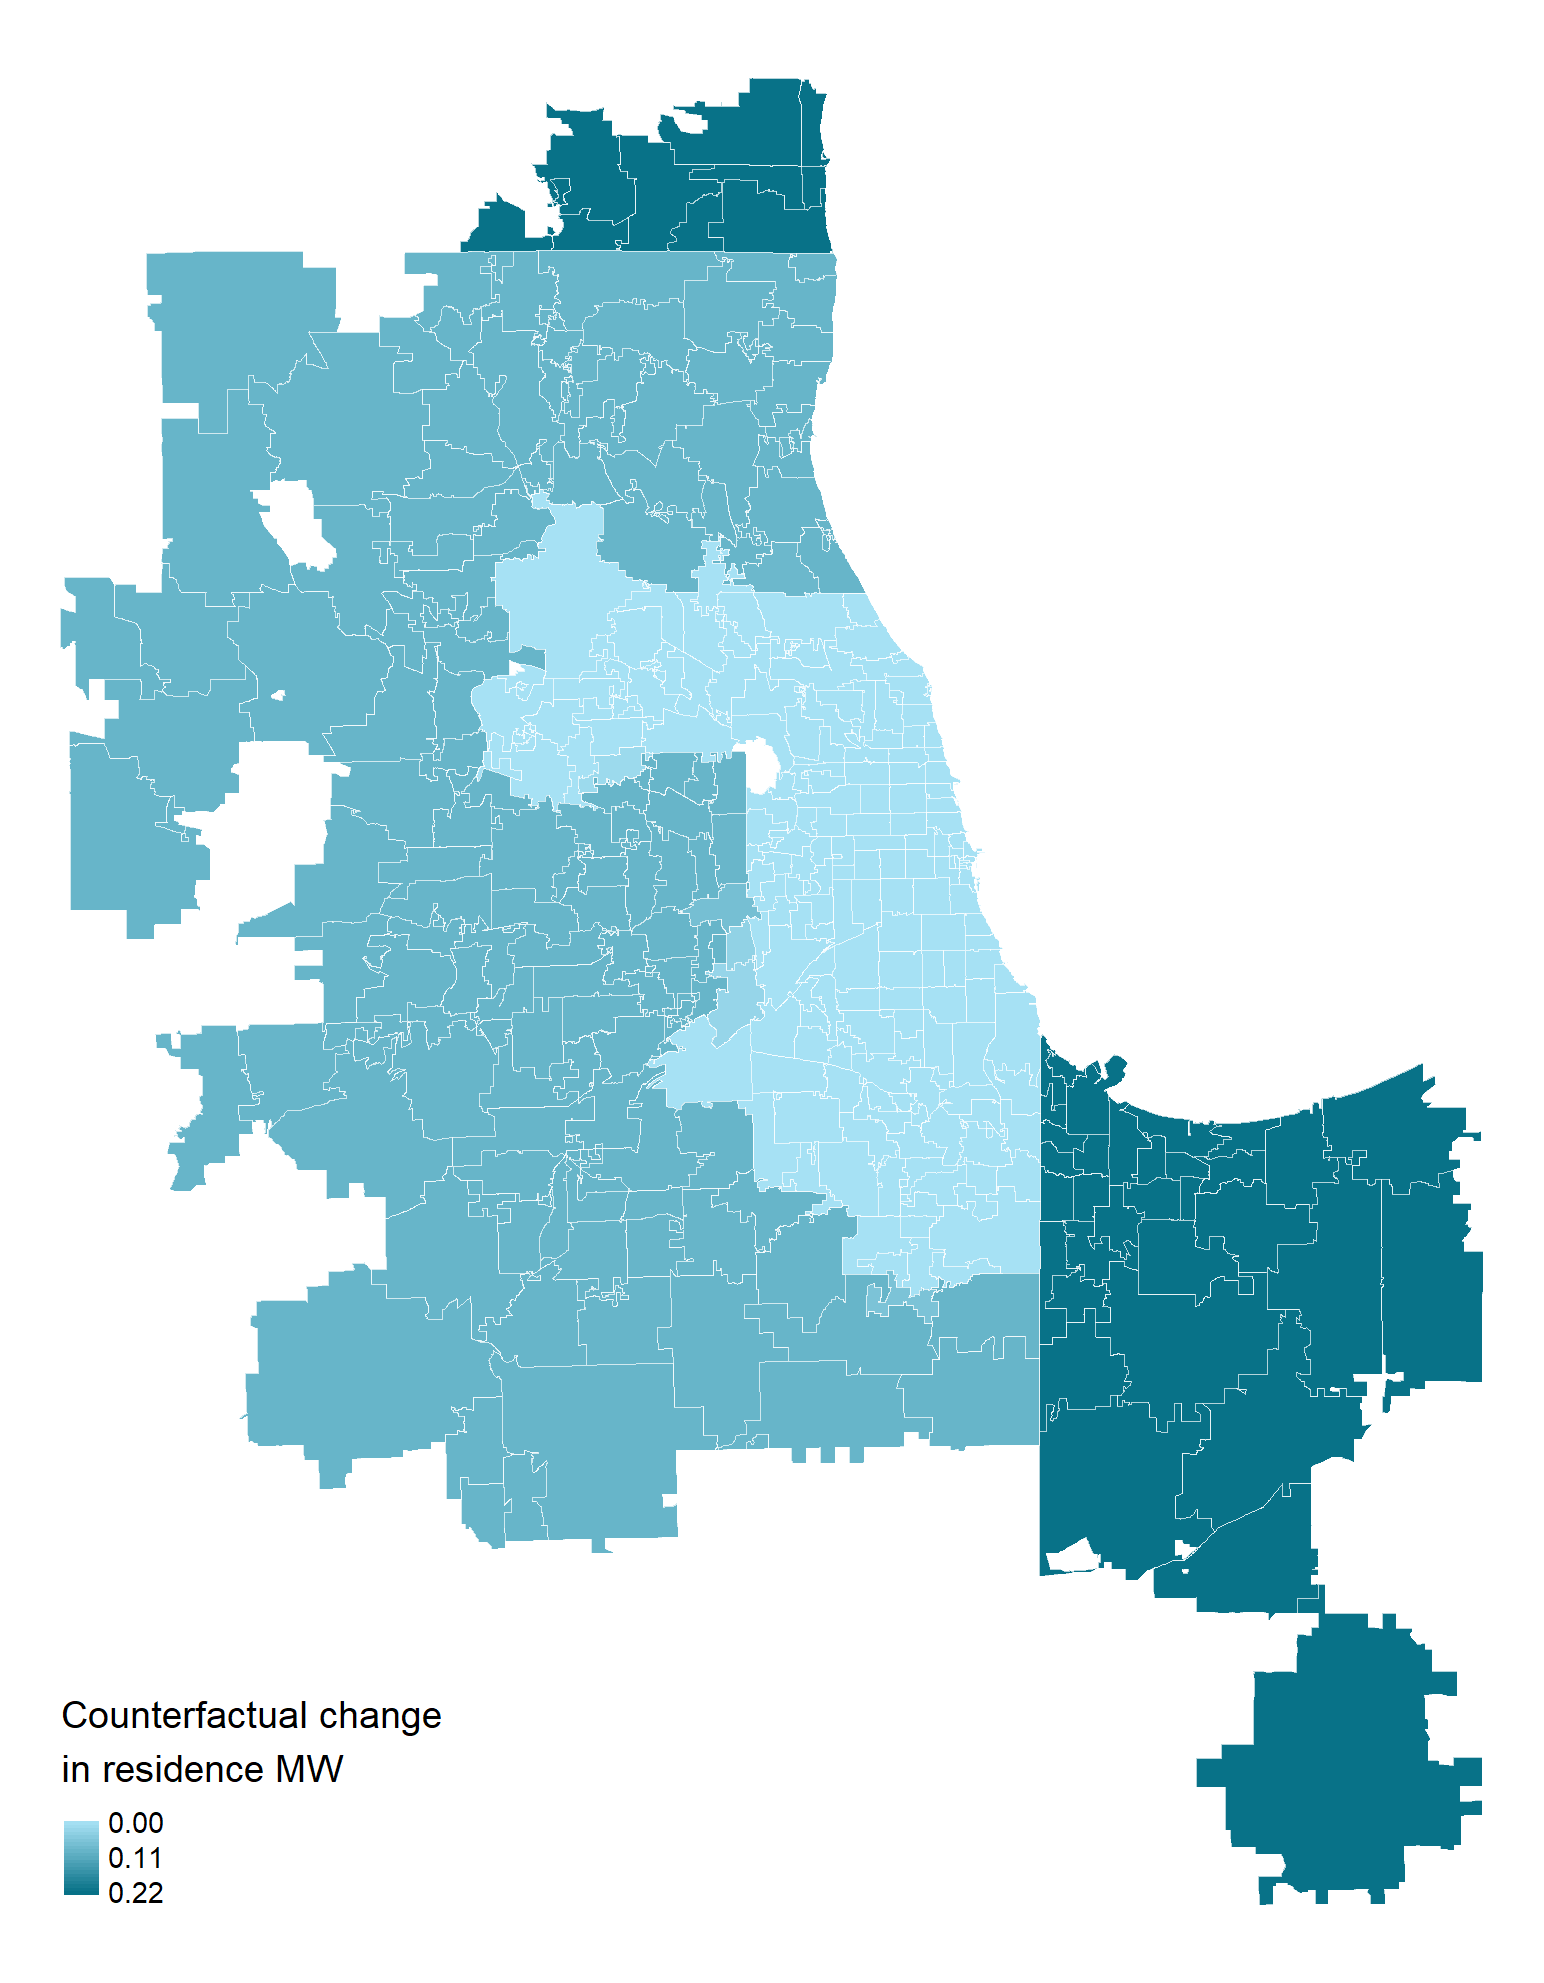
\includegraphics[width = 1\textwidth]
            {counterfactuals/output/chicago_d_mw_res.png}
    \end{subfigure}%
    \begin{subfigure}{.49\textwidth}
        \caption*{Changes in workplace MW}
        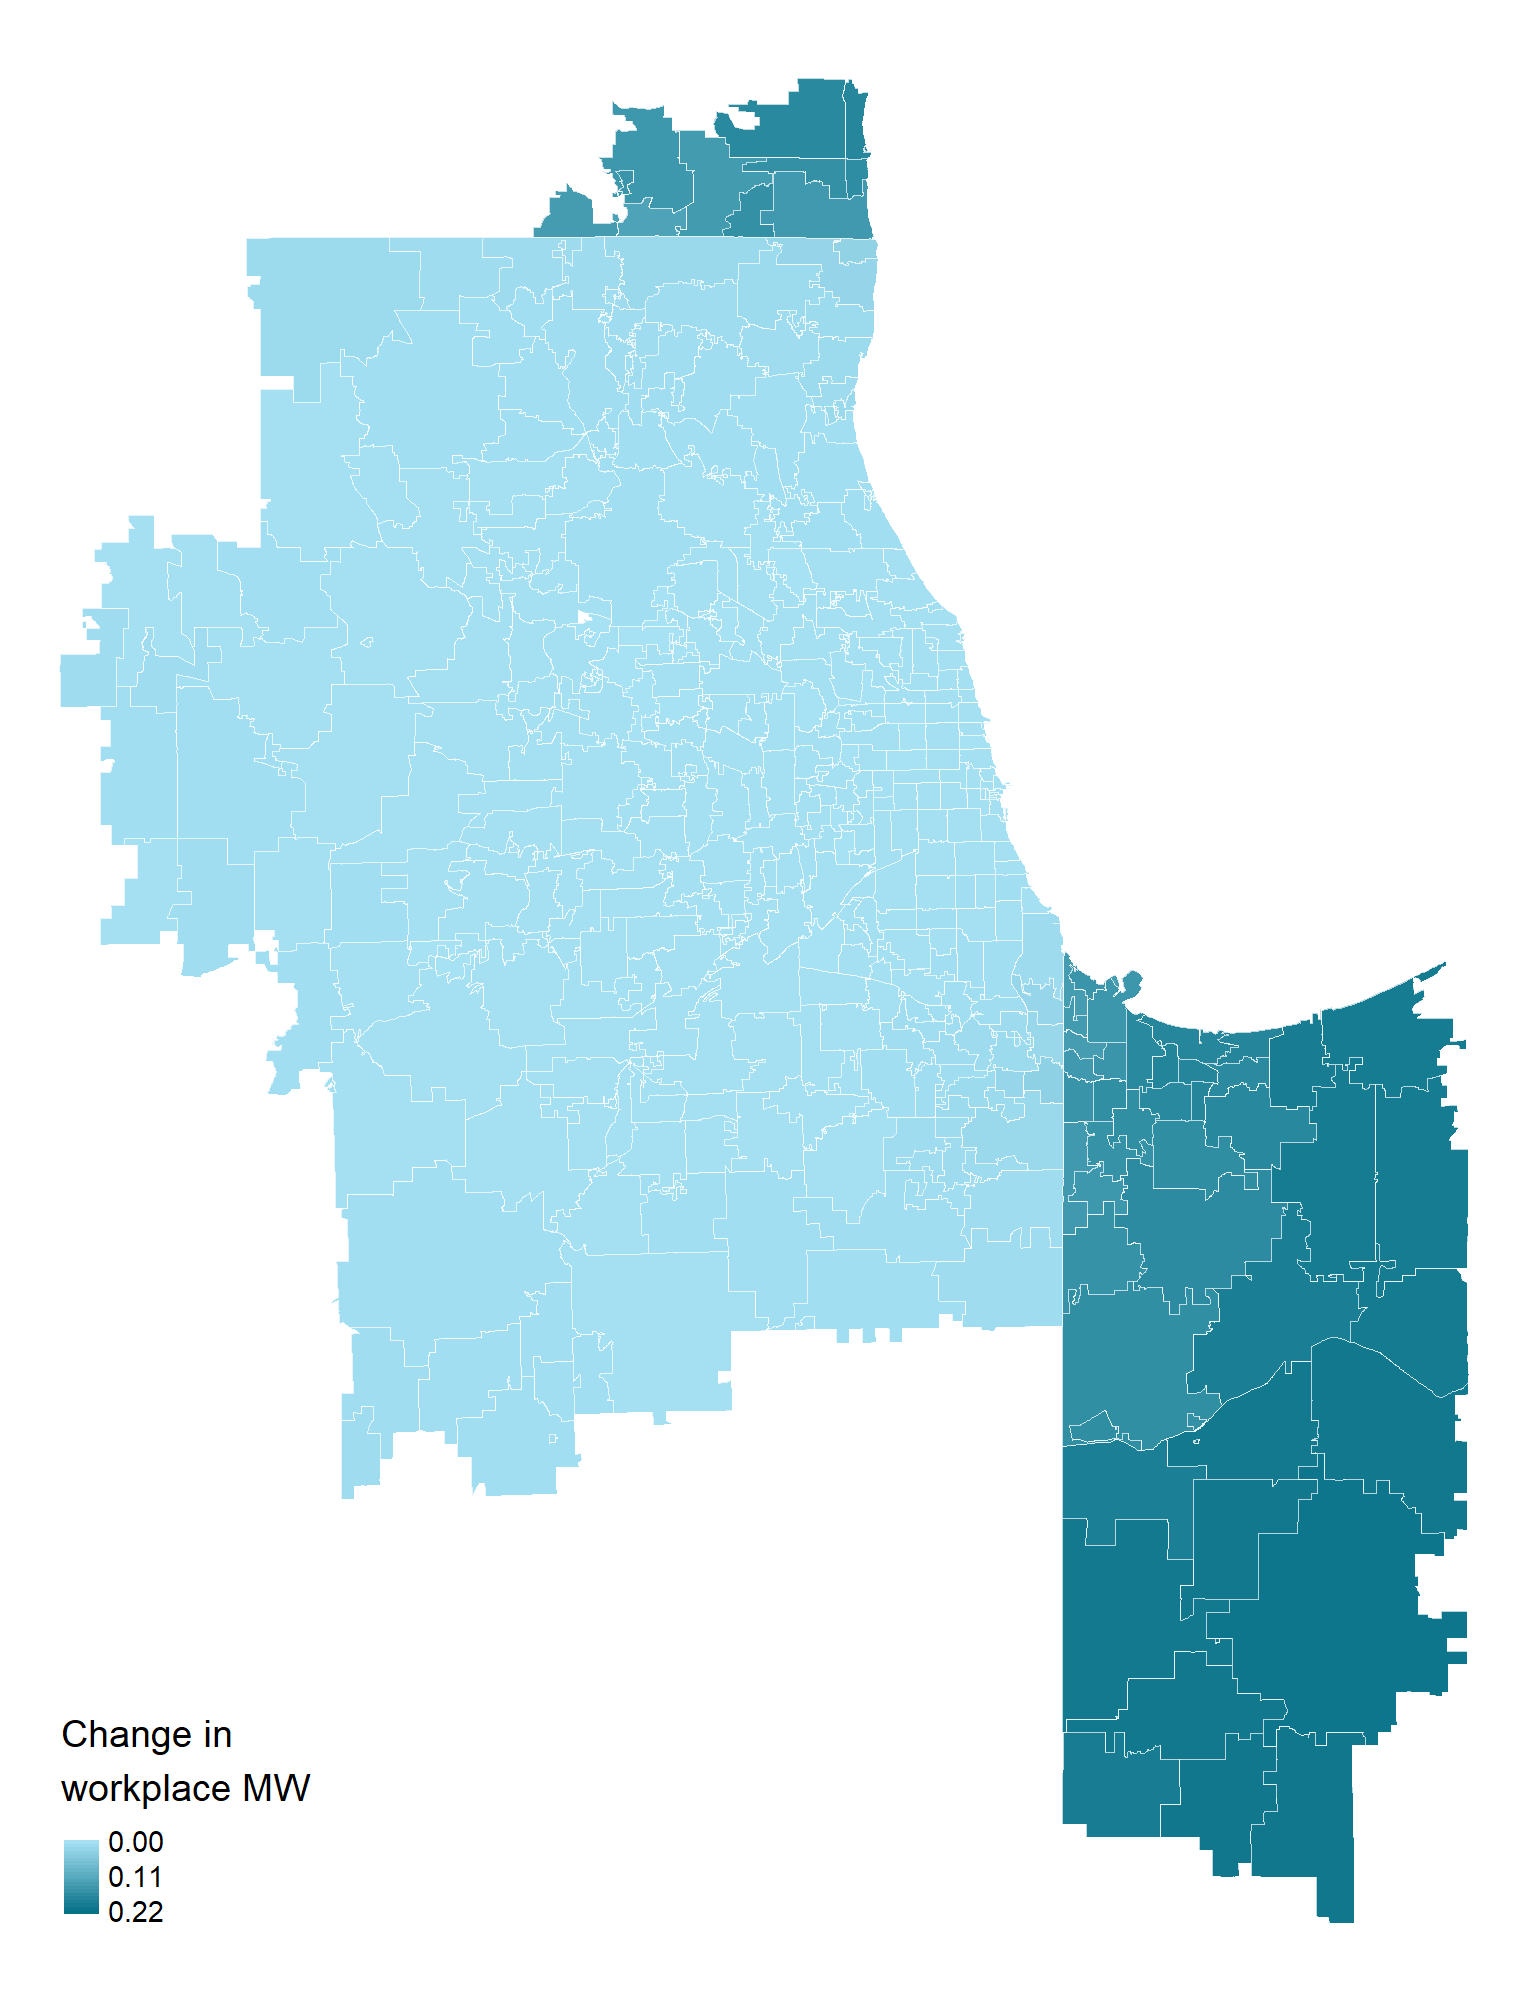
\includegraphics[width = 1\textwidth]
            {counterfactuals/output/chicago_d_mw_wkp.png}
    \end{subfigure}

    \begin{minipage}{.95\textwidth} \footnotesize
        \vspace{3mm}
        Notes:
        Data are from the minimum wage panel described in 
        Section \ref{sec:data_mw_panel} and from LODES.
        The figures map changes in the residence and workplace MW measures 
        generated by a counterfactual increase to \$9 in the federal MW in 
        January 2020, holding constant other MW policies at their December 2019 
        levels.
    \end{minipage}
\end{figure}


\clearpage

\begin{figure}[h!]
    \centering
    \caption{Sample of ZIP codes in Zillow data vs.\ population density}
    \label{fig:map_zillow_sample}

    \begin{subfigure}{1\textwidth}
        \caption{Zillow ZIP codes}
        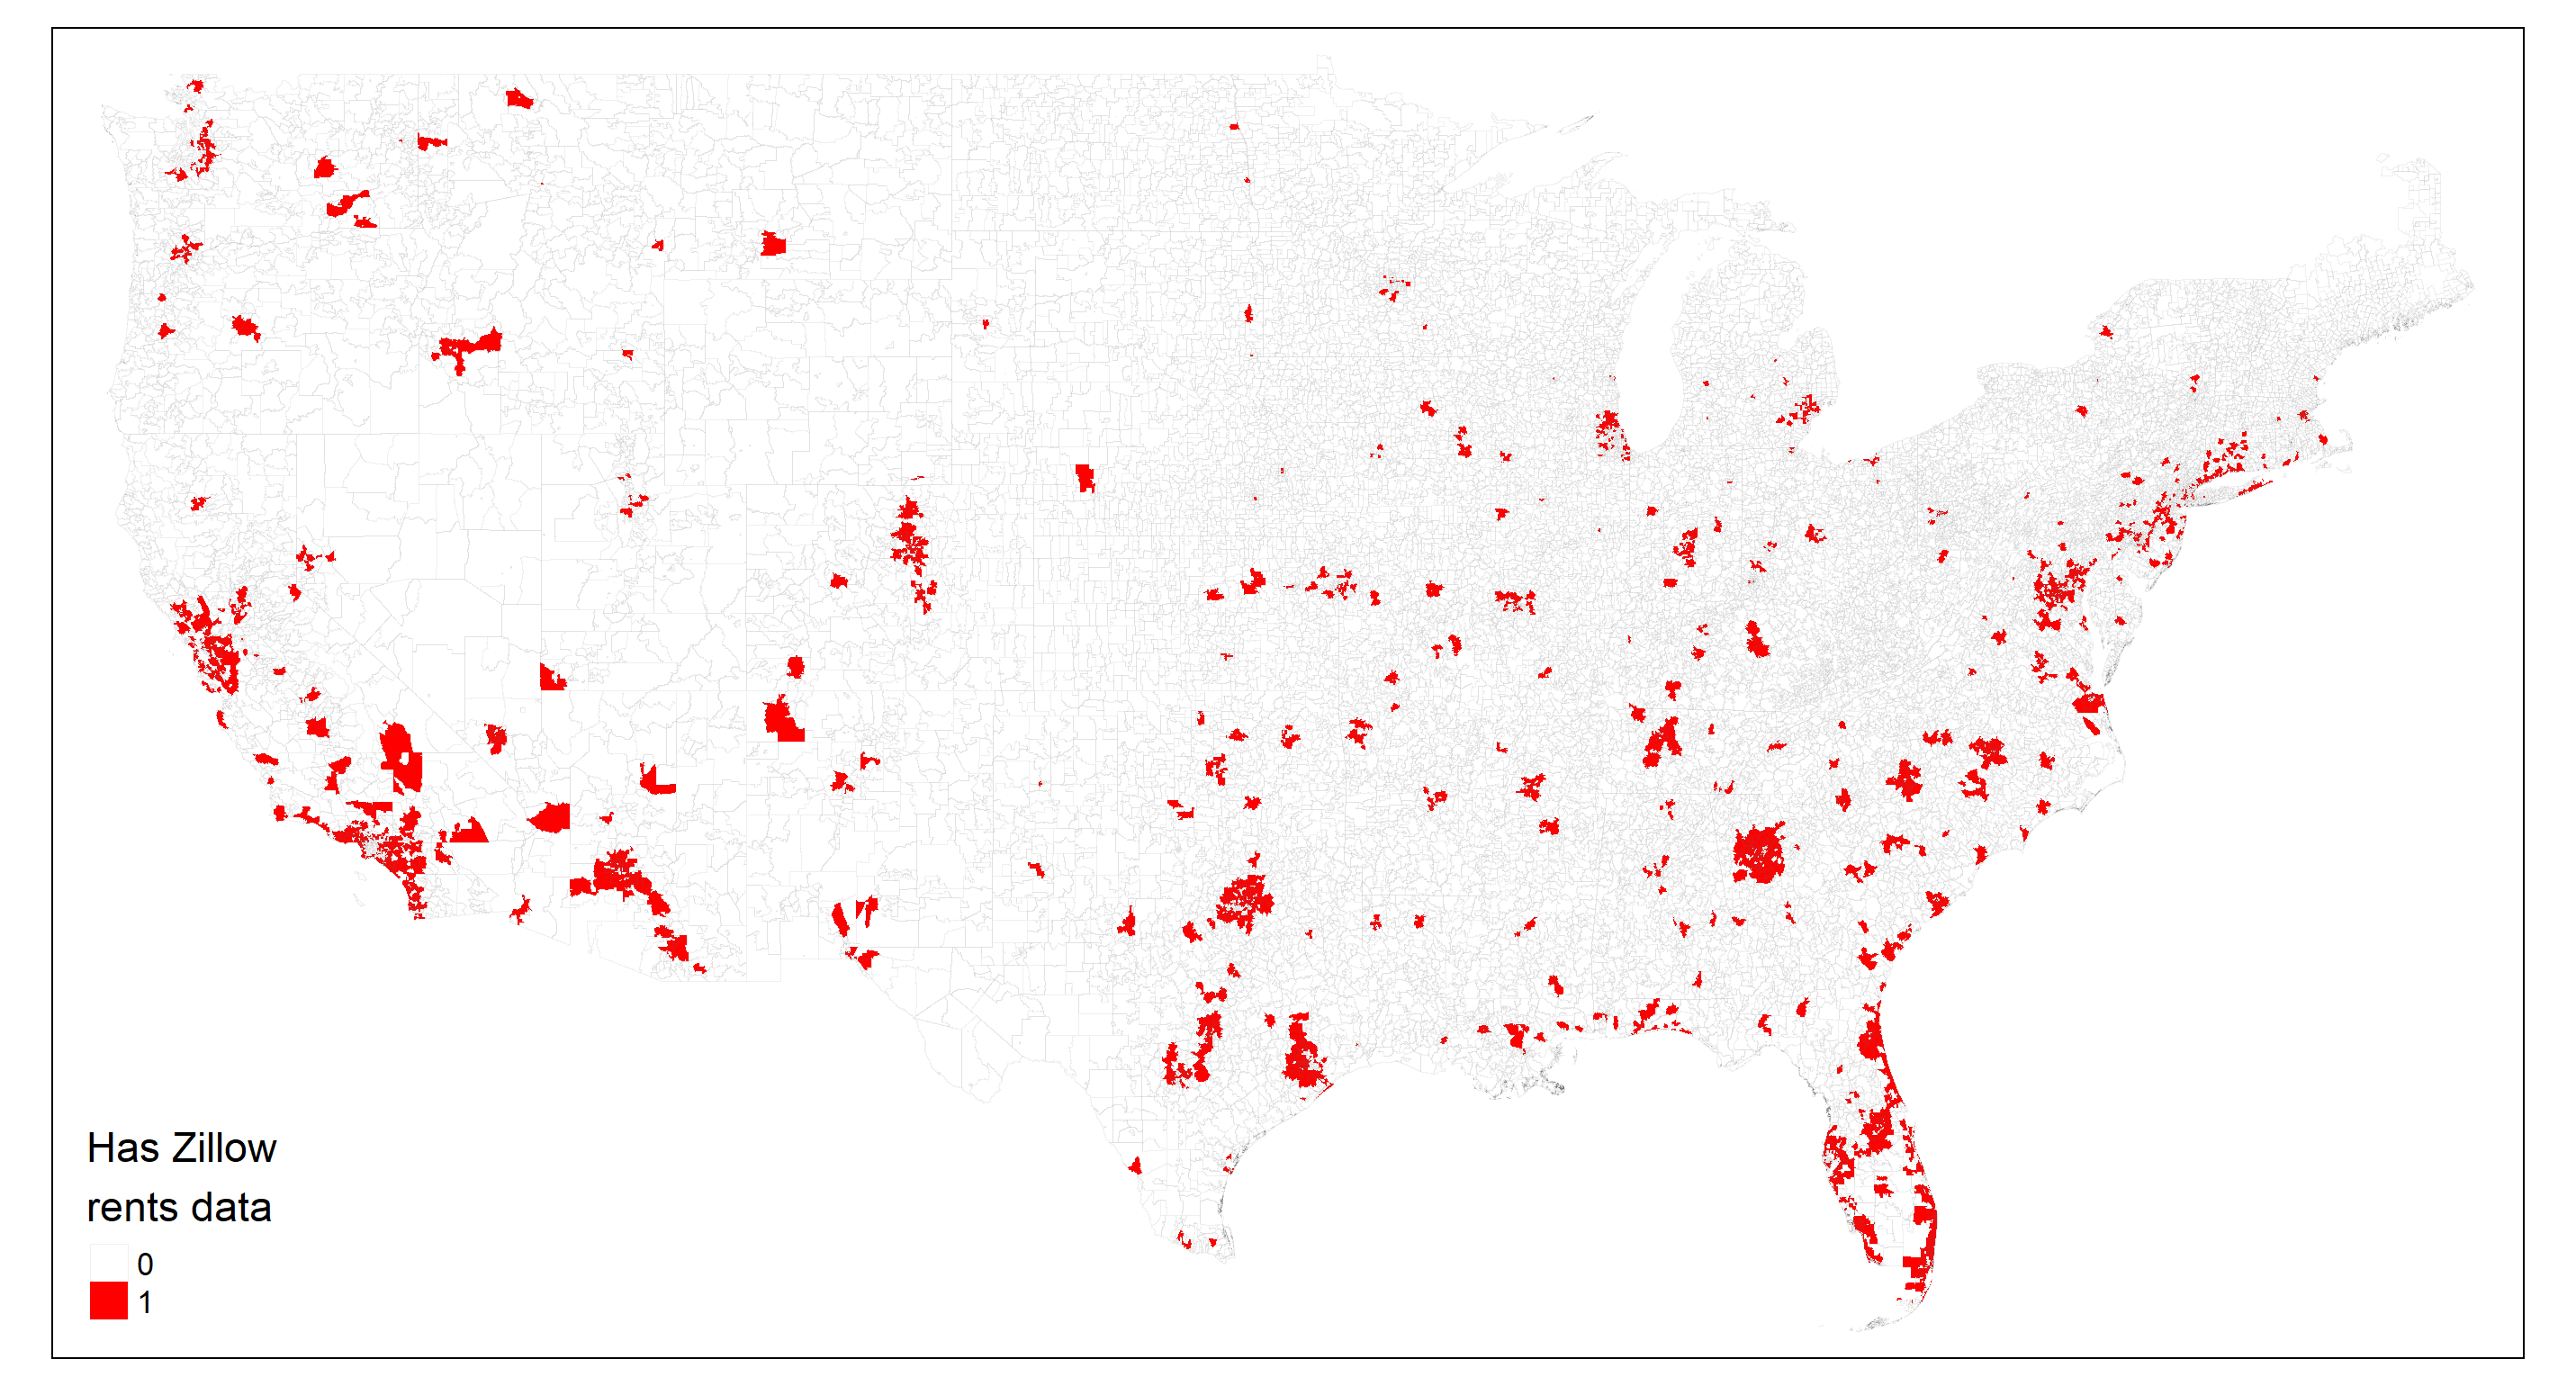
\includegraphics[width = 0.95\textwidth]
            {maps_US/output/USPS_zipcodes_zillow_data.png}
    \end{subfigure}\\
    \begin{subfigure}{1\textwidth}
        \caption{Population Density}
        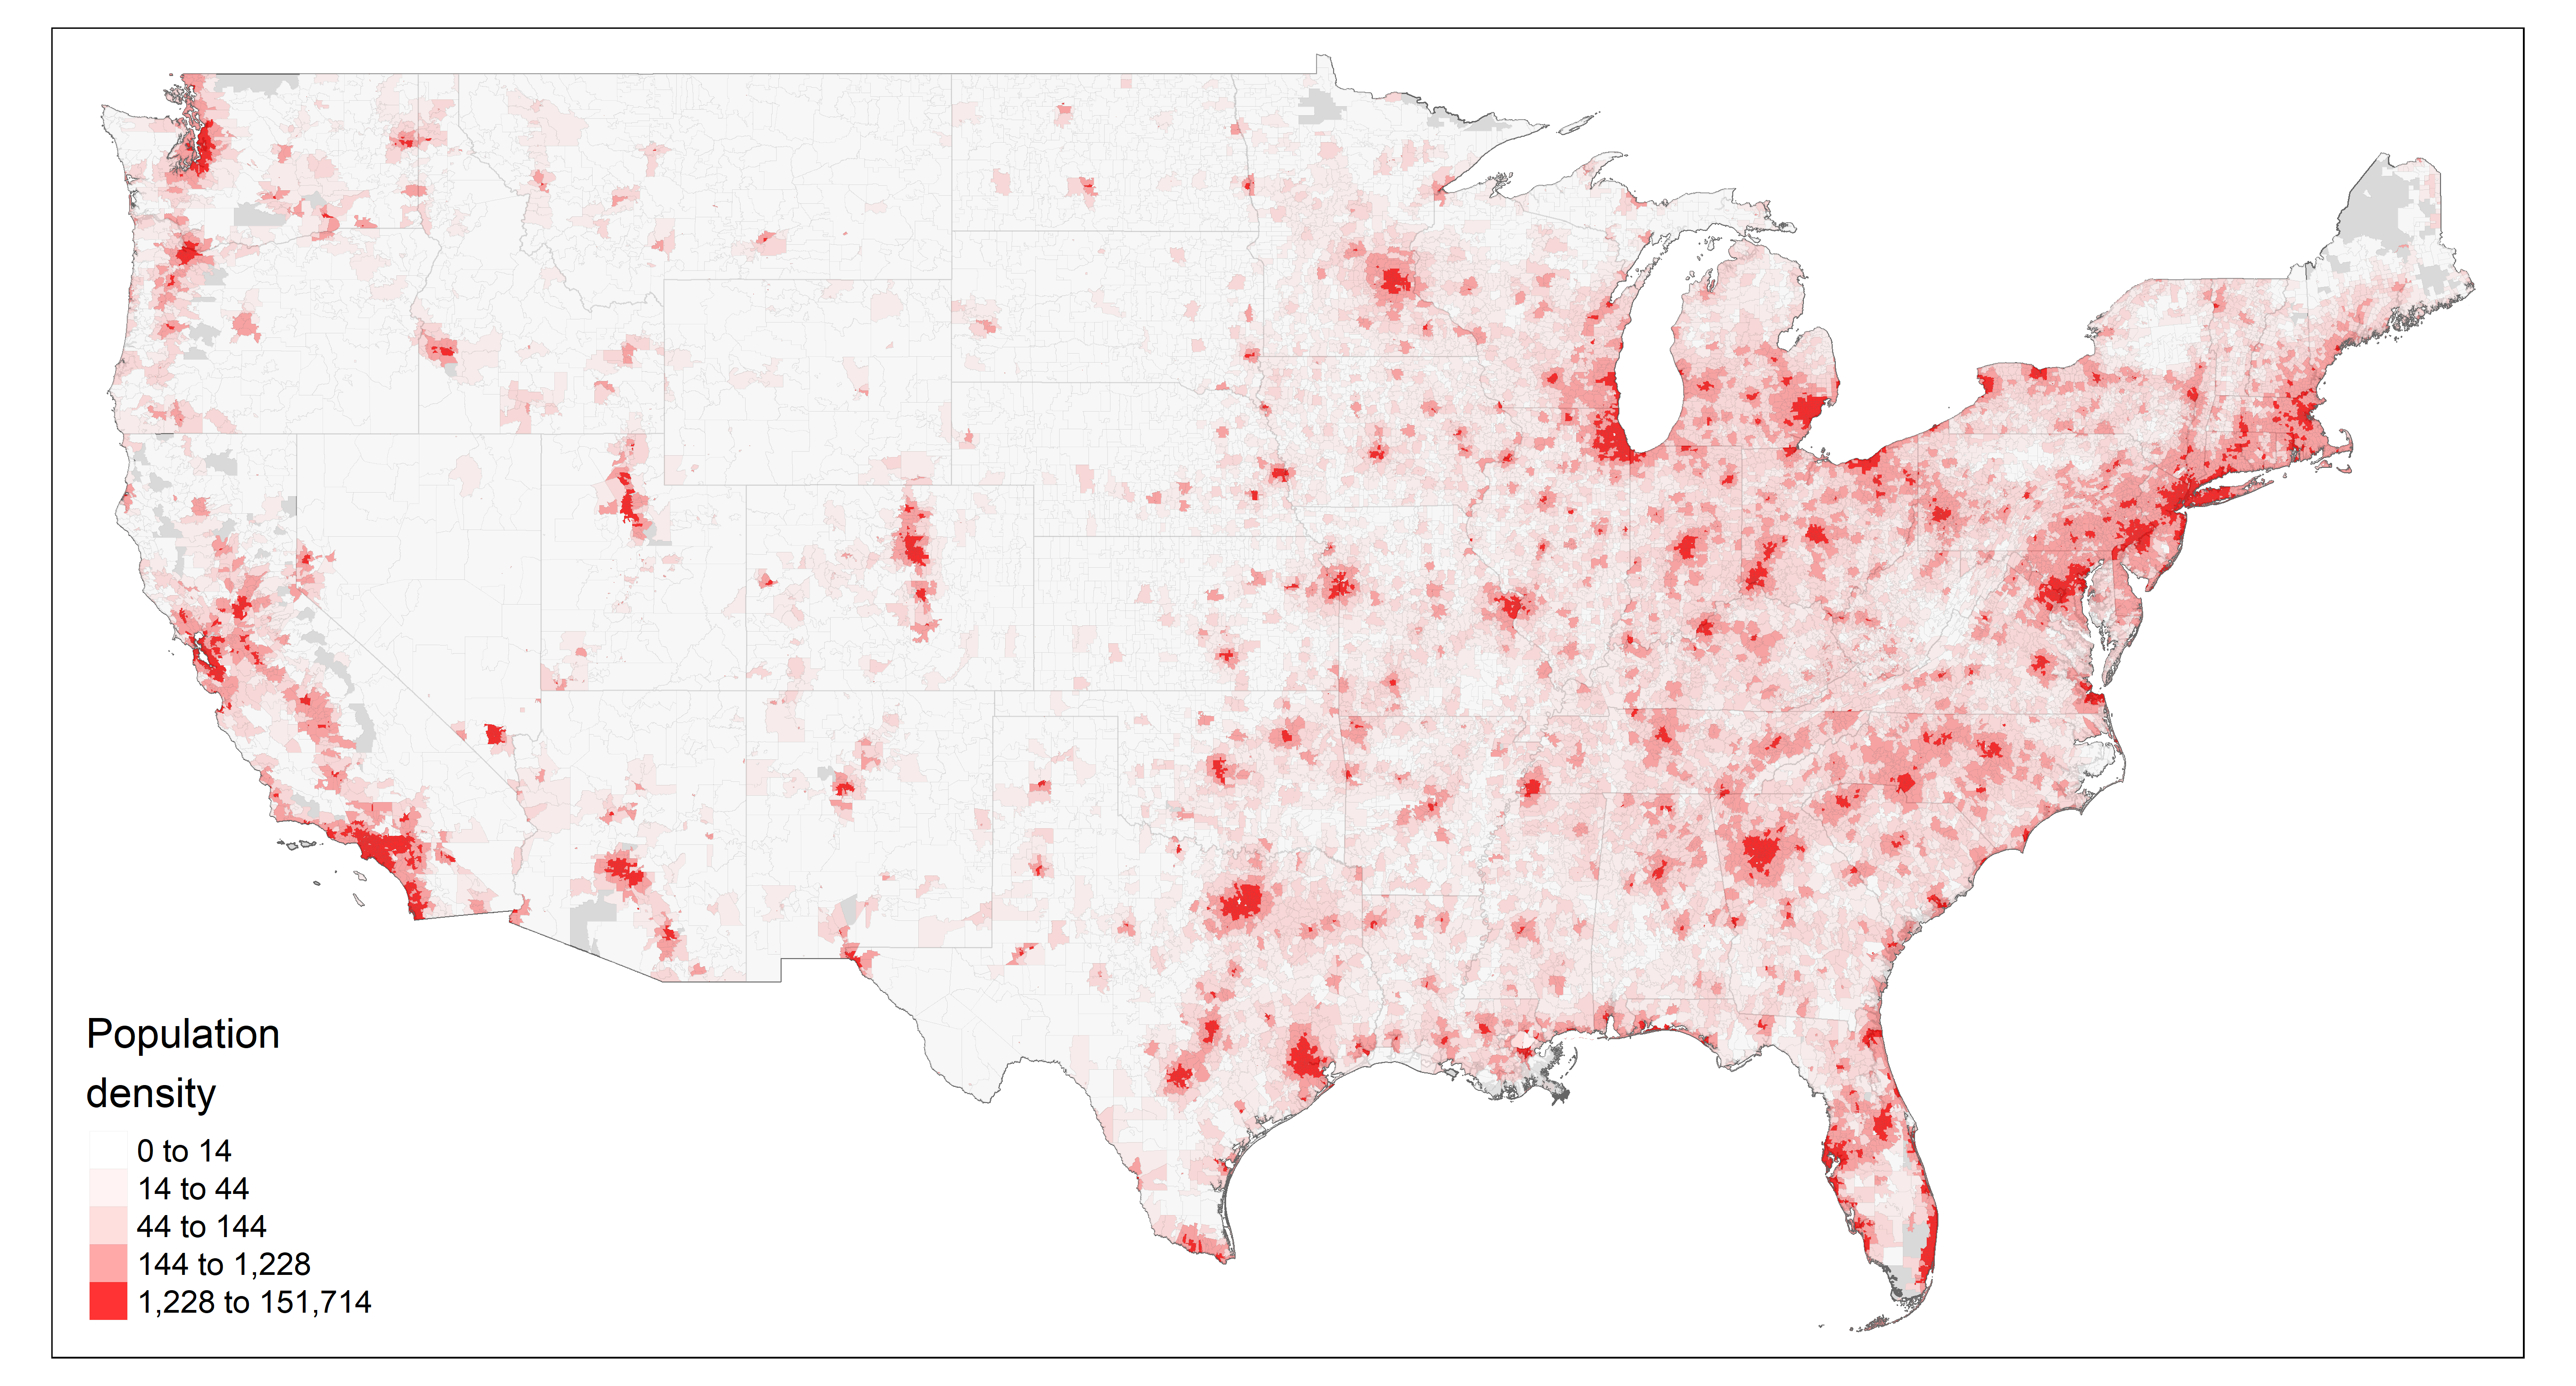
\includegraphics[width = 0.95\textwidth]
            {maps_US/output/USPS_zipcodes_pop_density.png}
    \end{subfigure}

    \begin{minipage}{.95\textwidth} \footnotesize
        \vspace{3mm}
        Notes:
        Data are from \textcite{ZillowData} and CENSO (YYYY).
        %%
        %% SH: Add cite of census data used in the map
        %%
        The figure compares the USPS ZIP codes available in Zillow to the 
        population density.
        Panel (a) shows the sample of the ZIP codes that have rents data in the 
        SFCC category at any point in the period 2010--2019.
        Panel (b) shows quintiles of population density, measured in people per
        square kilometer.
        %%
        %% SH: Is this the right unit of pop density?
        %%
        %%  Comments on map, after seeing it in PDF
        %%     Can we add the unit of pop density to the map?
        %%     Can we drop the box around the maps?
        %%     Can we make the white fill color coincide with the background white?
        %% 
    \end{minipage}
\end{figure}

\clearpage

\begin{figure}[h!]
    \centering
    \caption{Time trends in rents according to Zillow and SAFMR}
    \label{fig:trend_zillow_safmr}

	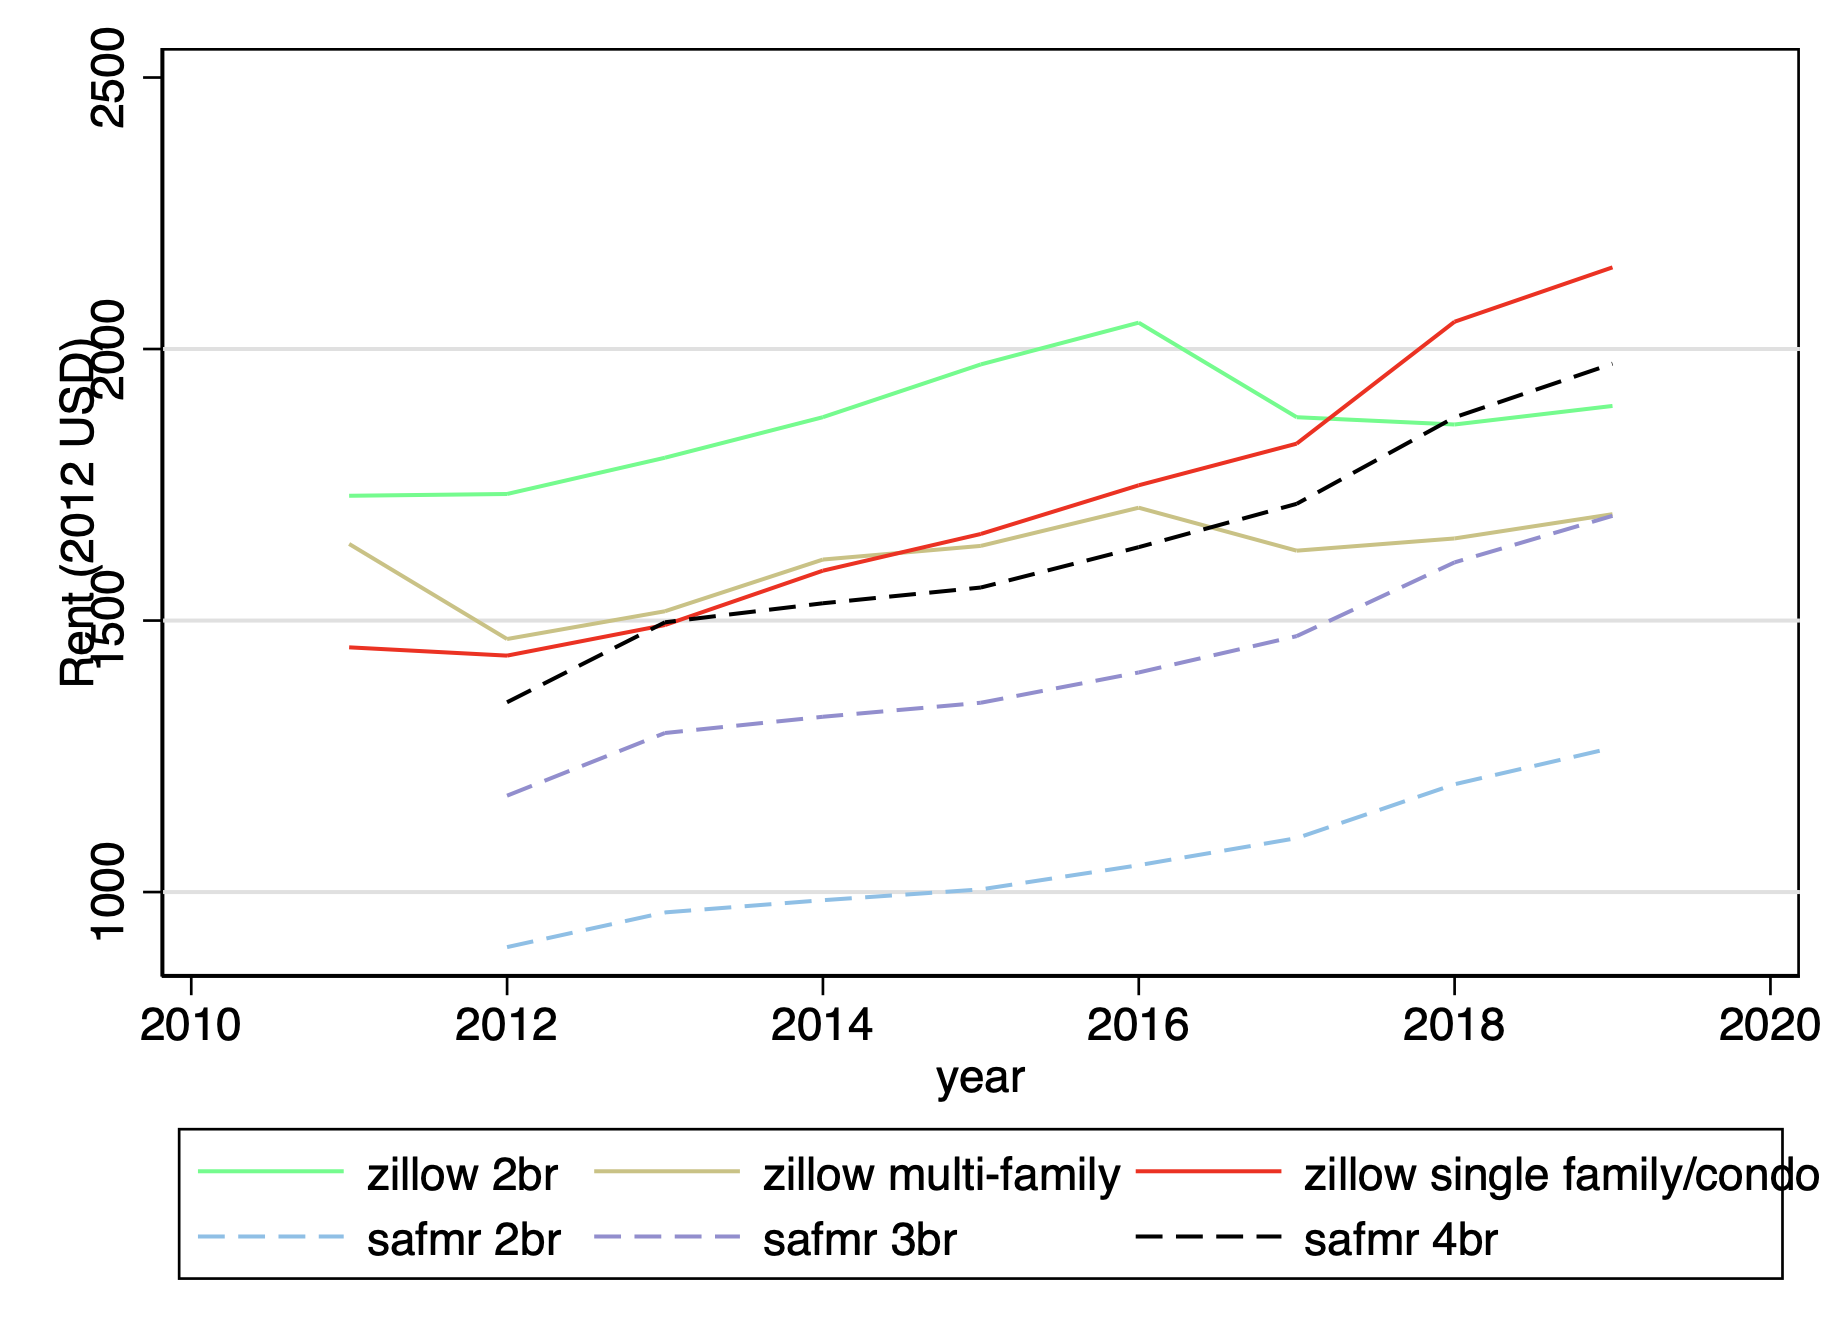
\includegraphics[width = 0.8\textwidth]
        {zillow_benchmark/output/trend_zillow_safmr_zipcode_m1.png}

    \begin{minipage}{.95\textwidth} \footnotesize
        \vspace{3mm}
        Notes:
        Data are from \textcite{ZillowData} and Small Area Fair Market Rents 
        (\citeyear[SAFMR]{hudSAFMR}).
        The figure compares the evolution of the median rental value in Zillow
        to three SAFMRs series, for 2, 3, and 4 or more bedrooms.
    \end{minipage}
\end{figure}

\clearpage
\begin{figure}[h!]
    \centering
    \caption{Spatial Distribution of Minimum Wage Changes}
    \label{fig:map_mw_perc_changes}

    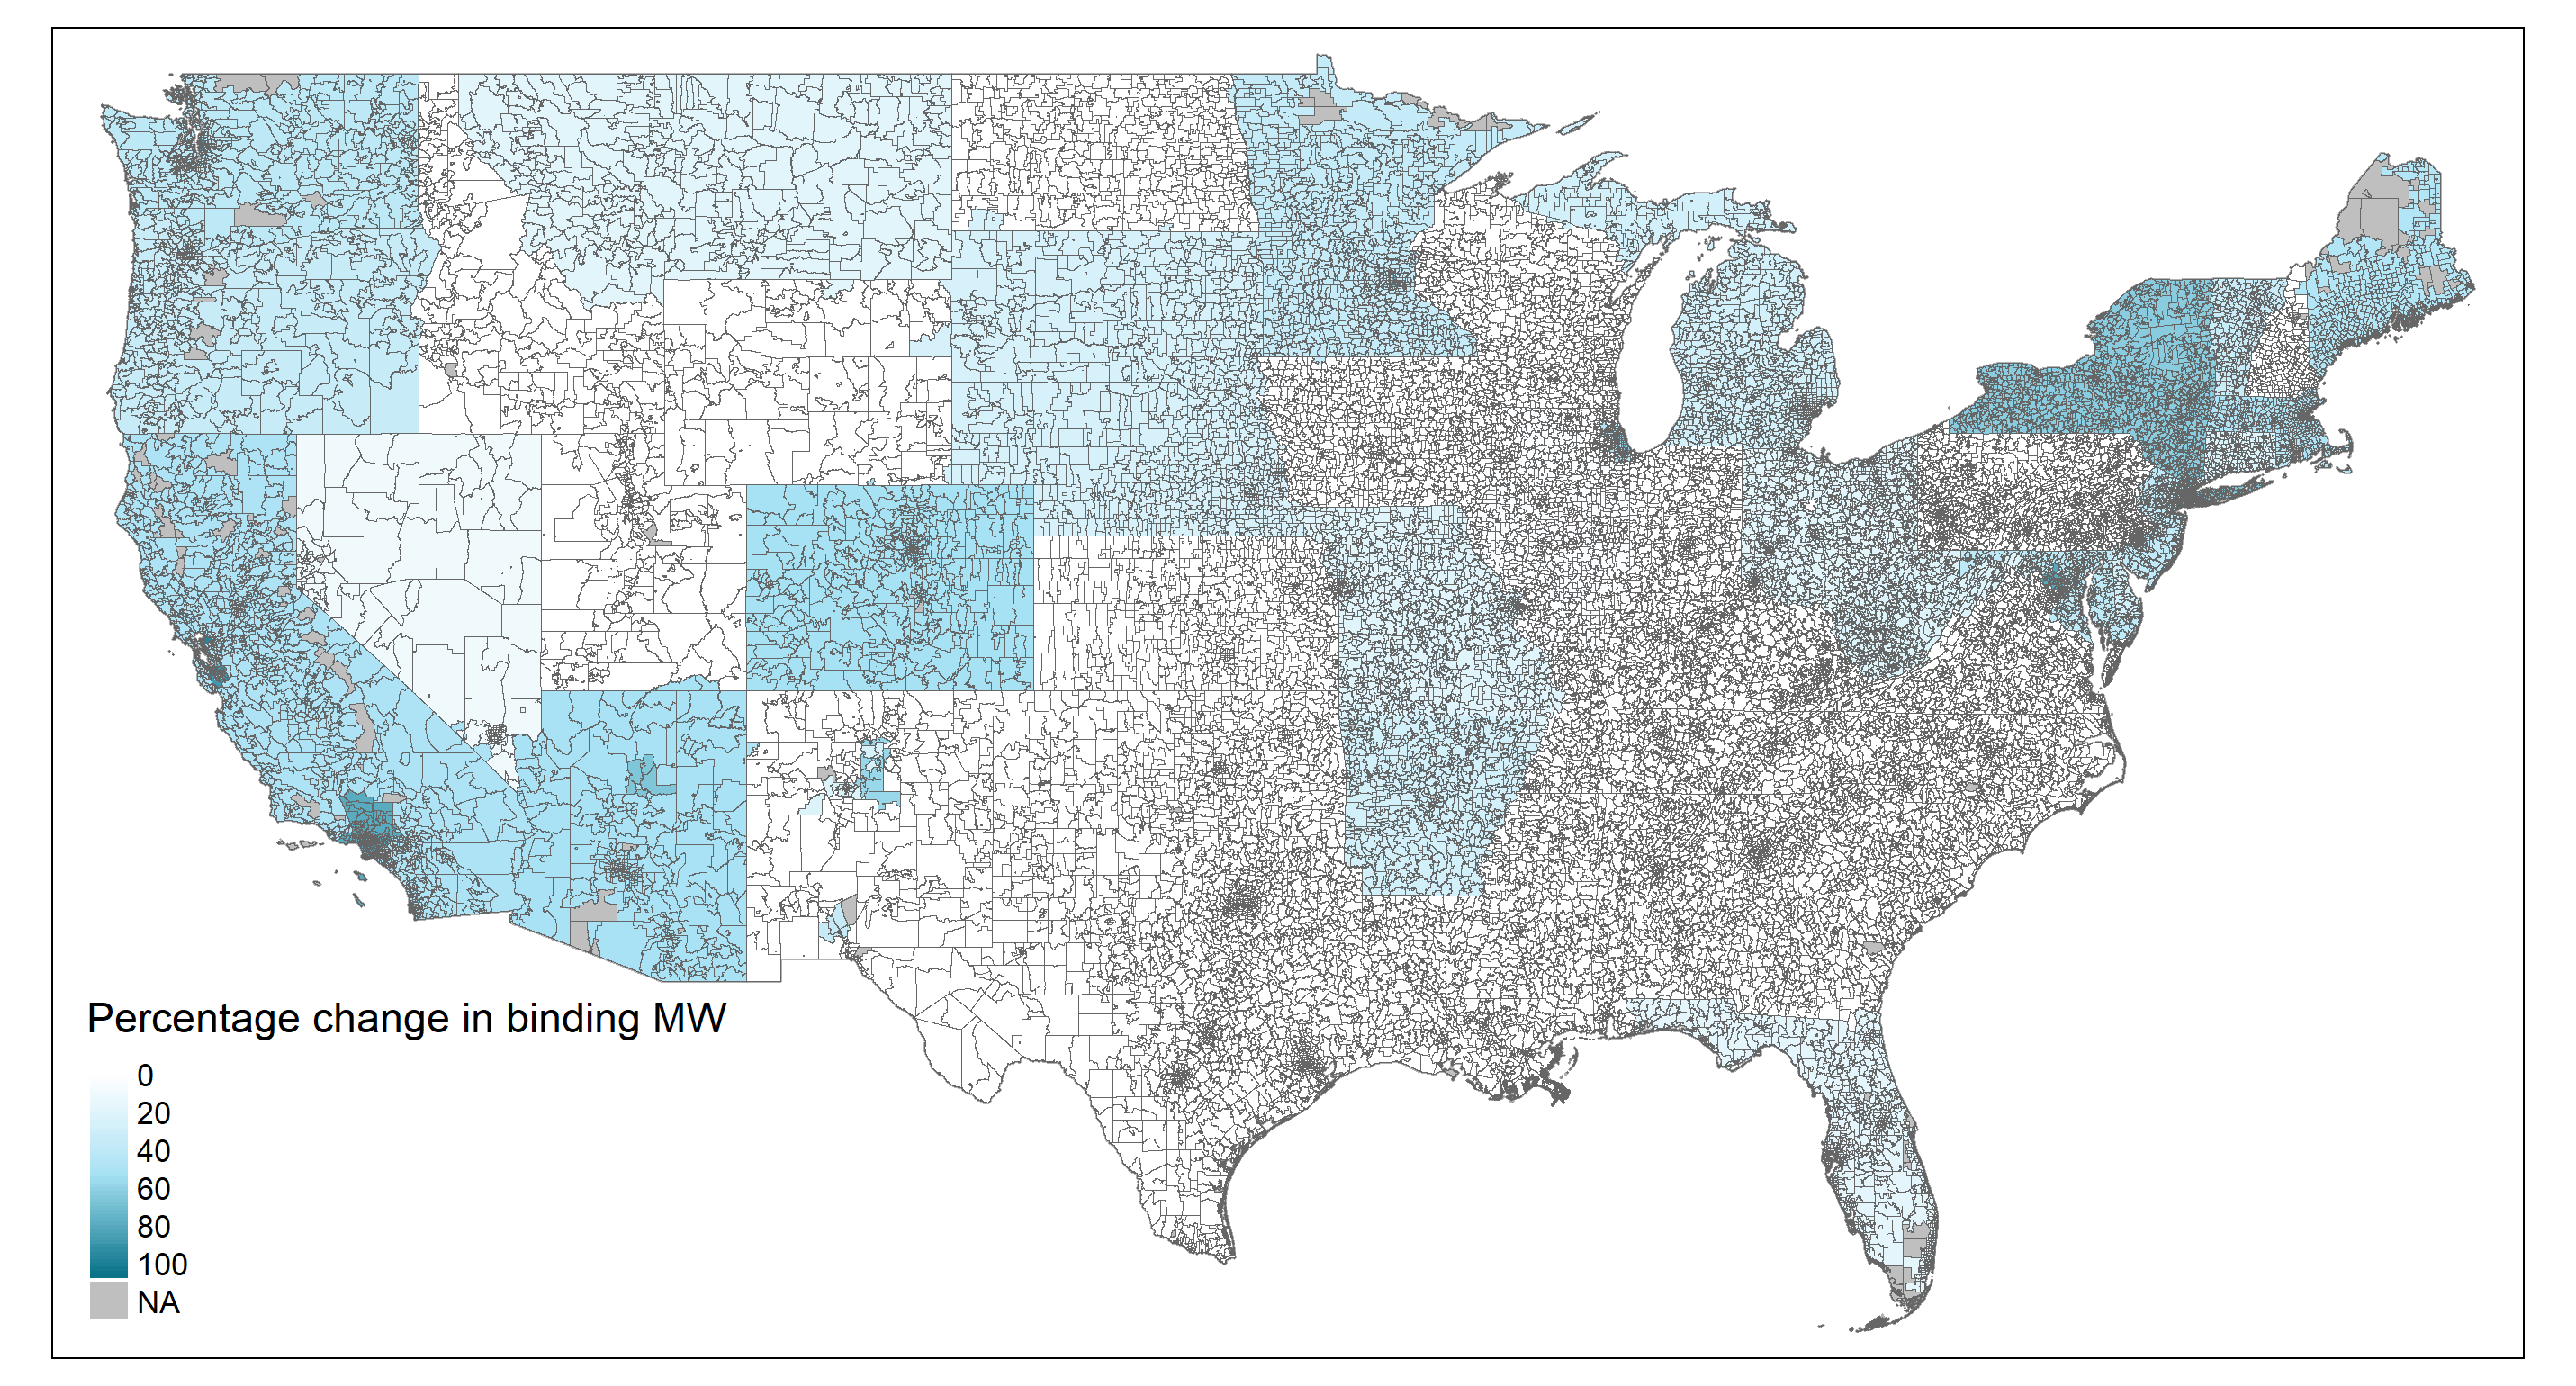
\includegraphics[width = 0.95\textwidth]
        {maps_mw_long_run/output/USchange_perc_actual_mw.png}

    \begin{minipage}{.95\textwidth} \footnotesize
        \vspace{3mm}
        Notes: 
        The figure maps the percentage change in the statutory minimum wage 
        level in each USPS ZIP code from January 2010 to December 2019.
    \end{minipage}
\end{figure}

\clearpage
\begin{figure}[h!]
    \centering
    \caption{Changes in rents in Chicago on July 2019}
    \label{fig:map_rents_chicago_jul2019}

    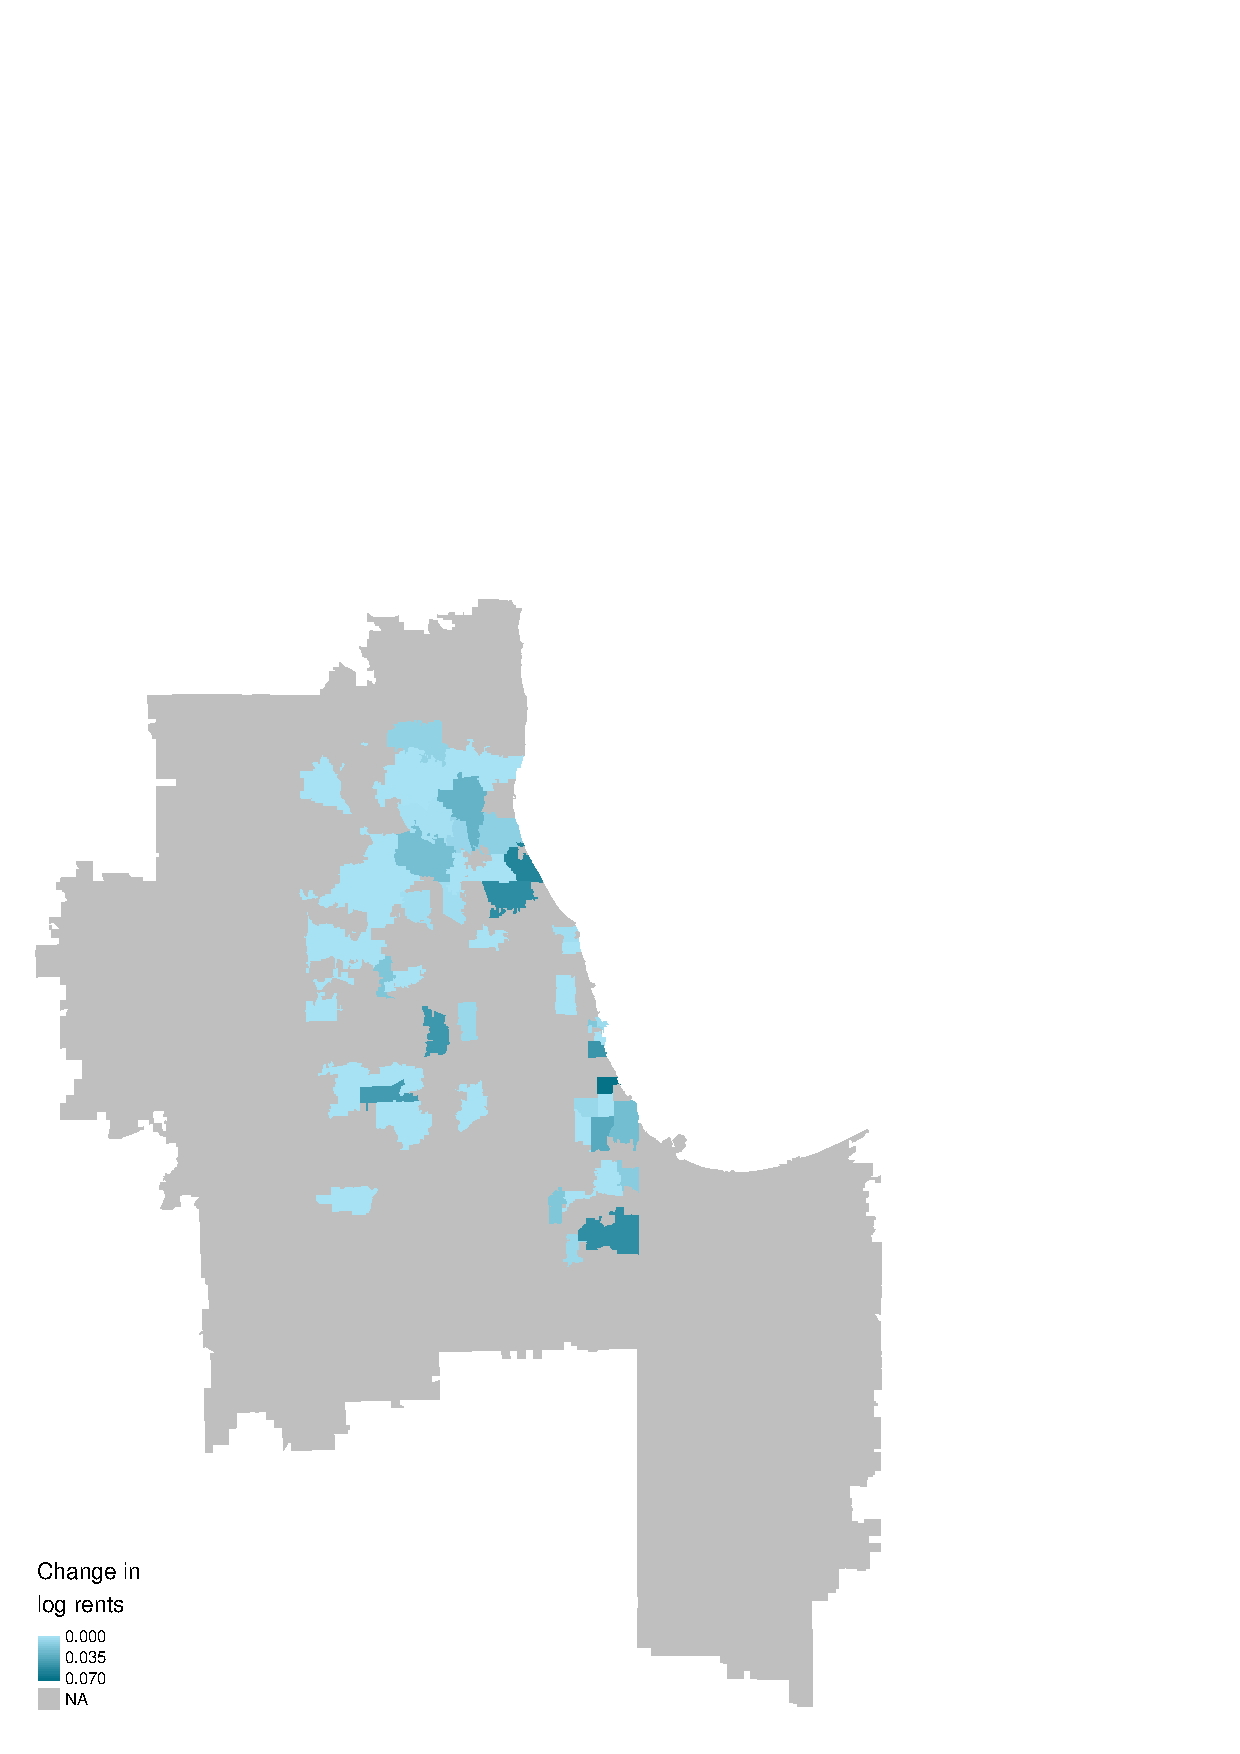
\includegraphics[width = 0.7\textwidth]
            {maps_events/output/chicago2019-6_rents}


    \begin{minipage}{.95\textwidth} \footnotesize
        \vspace{3mm}
        Notes: 
        Data are from Zillow \parencite{ZillowData}.
        The figure shows the change in the log of median rents in the SFCC 
        category in the month of June 2019 in ZIP codes located in the
        metropolitan area of Chicago.
    \end{minipage}
\end{figure}

\clearpage
\begin{figure}[h!]
    \centering
    \caption{Changes in residuals of baseline estimates in the 
             Chicago-Naperville-Elgin CBSA, July 2019}
    \label{fig:map_residuals_chicago_jul2019}

    \begin{subfigure}{0.5\textwidth}
        \centering
        \caption{Residualized workplace MW}
        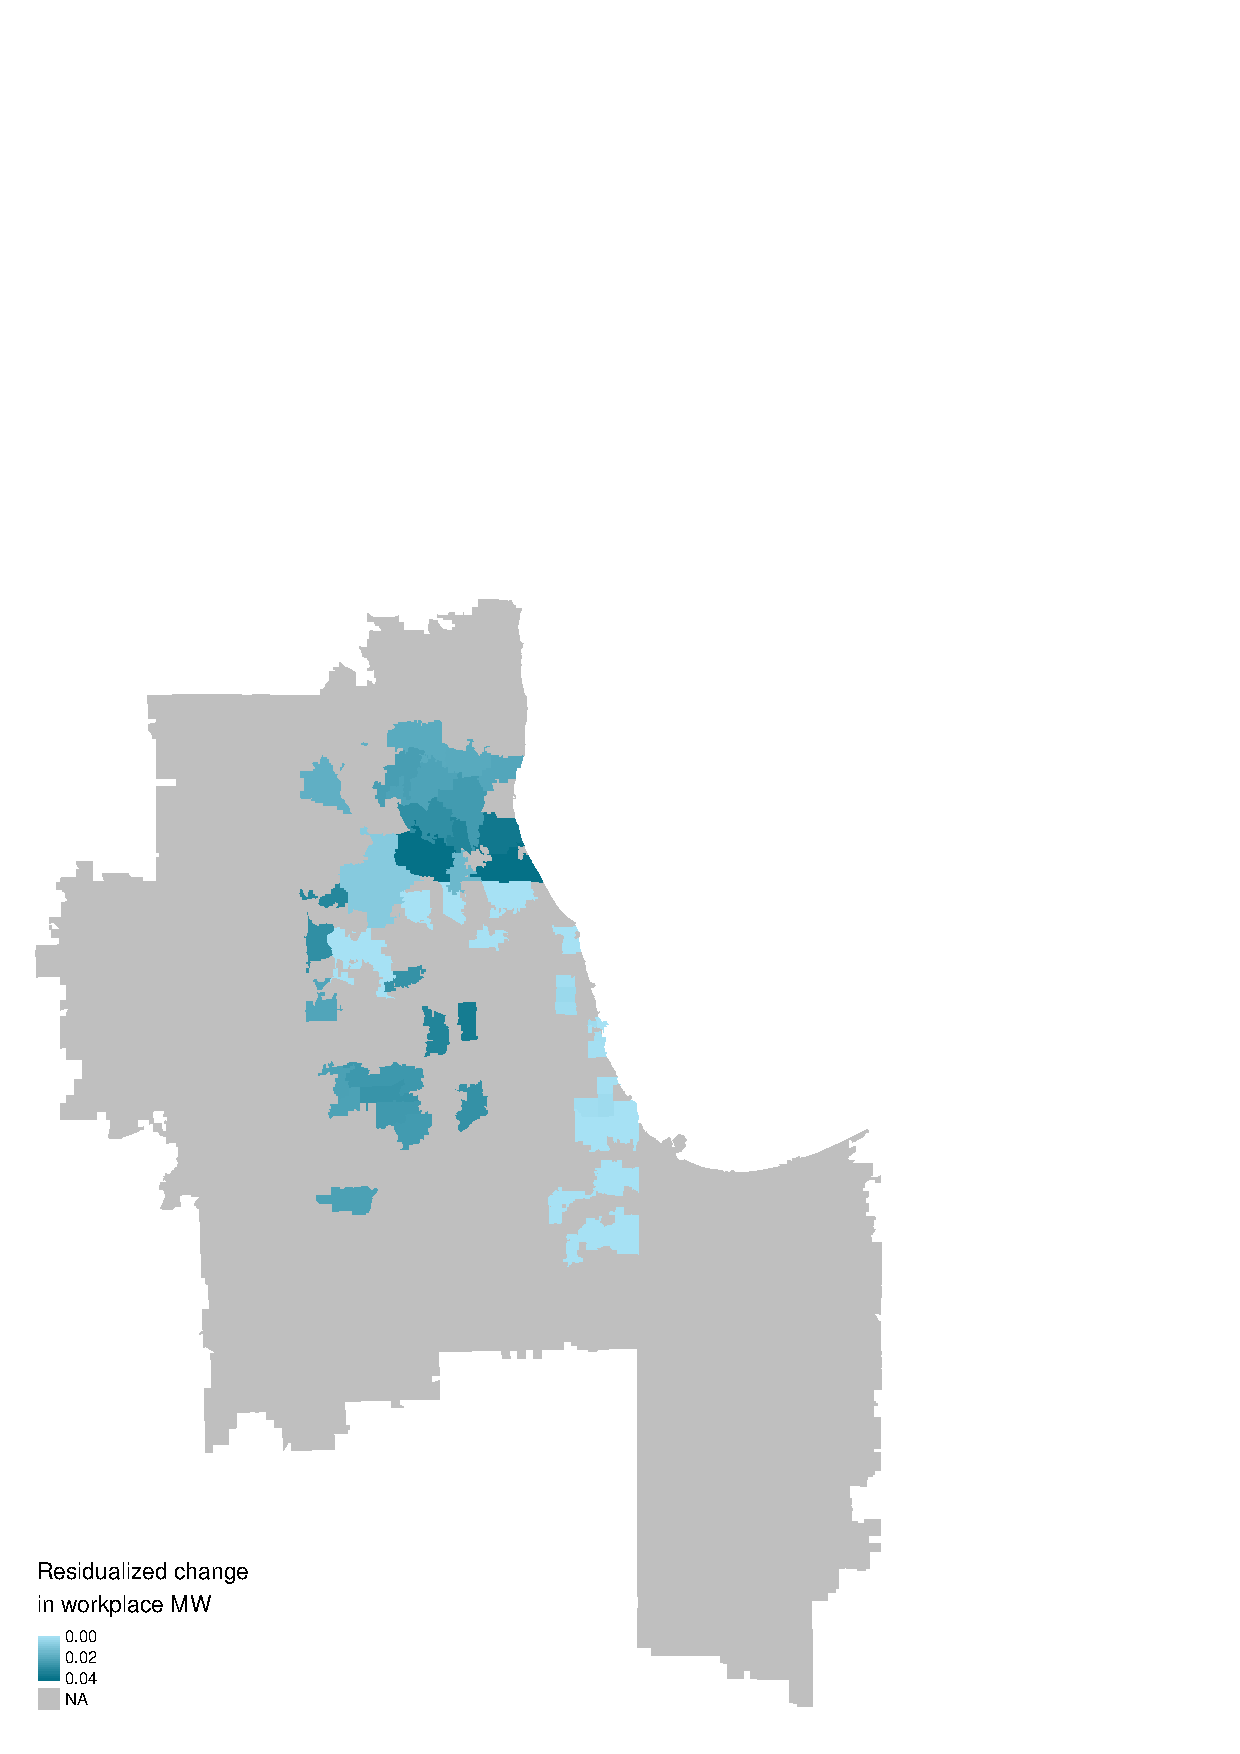
\includegraphics[width = 1\textwidth]
            {maps_events/output/chicago2019-6_r_wkp}
    \end{subfigure}%
    \begin{subfigure}{0.5\textwidth}
        \centering
        \caption{Residualized log rents}
        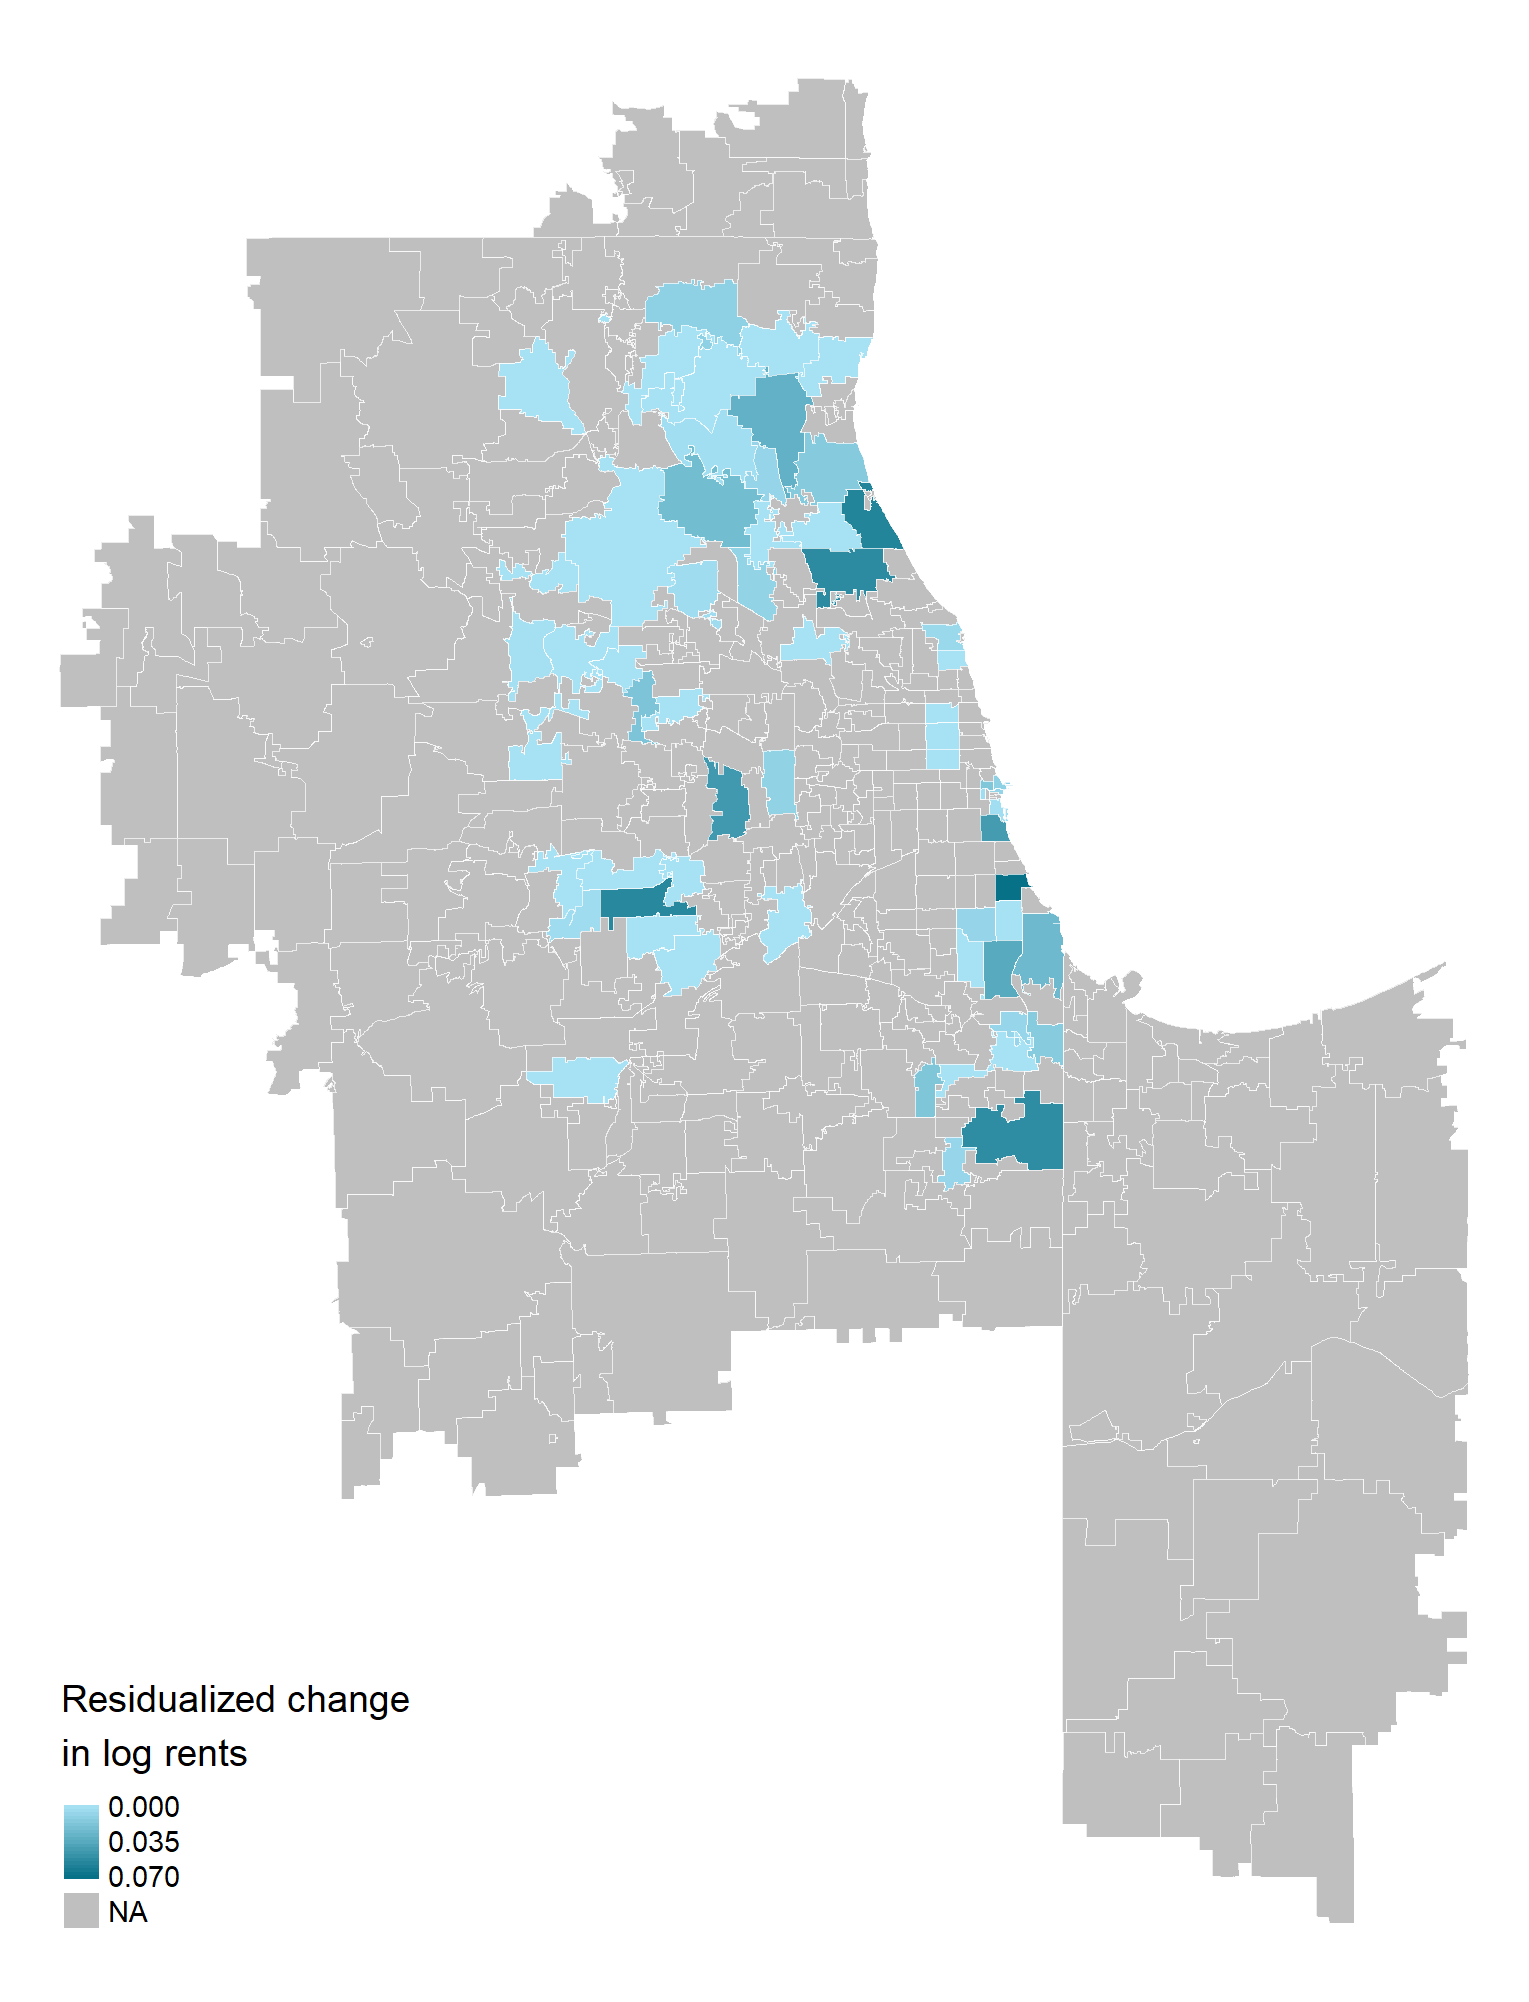
\includegraphics[width = 1\textwidth]
            {maps_events/output/chicago2019-6_r_rents}
    \end{subfigure}

    \begin{minipage}{.95\textwidth} \footnotesize
        \vspace{3mm}
        Notes: 
        Data are from the unbalanced estimation panel described in Section
        \ref{sec:data_final_panel}.
        Panel (a) maps the residuals of a regression of the change in the 
        workplace MW measure on the change in the residence MW measure, 
        including economic controls and year month fixed effects.
        Panel (b) maps the residuals of a regression of the change in log 
        rents on economic controls and year month fixed effects.
        The residence MW is defined as the log statutory MW in the same ZIP code.
        The workplace MW is defined as the statutory MW where the average 
        resident of the ZIP code works, constructed using LODES 
        origin-destination data.
        Economic controls from the QCEW include the change of the following 
        variables: the log of the average wage, the log of employment, and the 
        log of the establishment count for the sectors ``Information,''
        ``Financial activities,'' and ``Professional and business services.''
    \end{minipage}
\end{figure}

\clearpage

\begin{figure}[h!]
    \centering
    \caption{Estimates of the effect of the MW on rents, using County-month data}
    \label{fig:dynamic_county_month}

	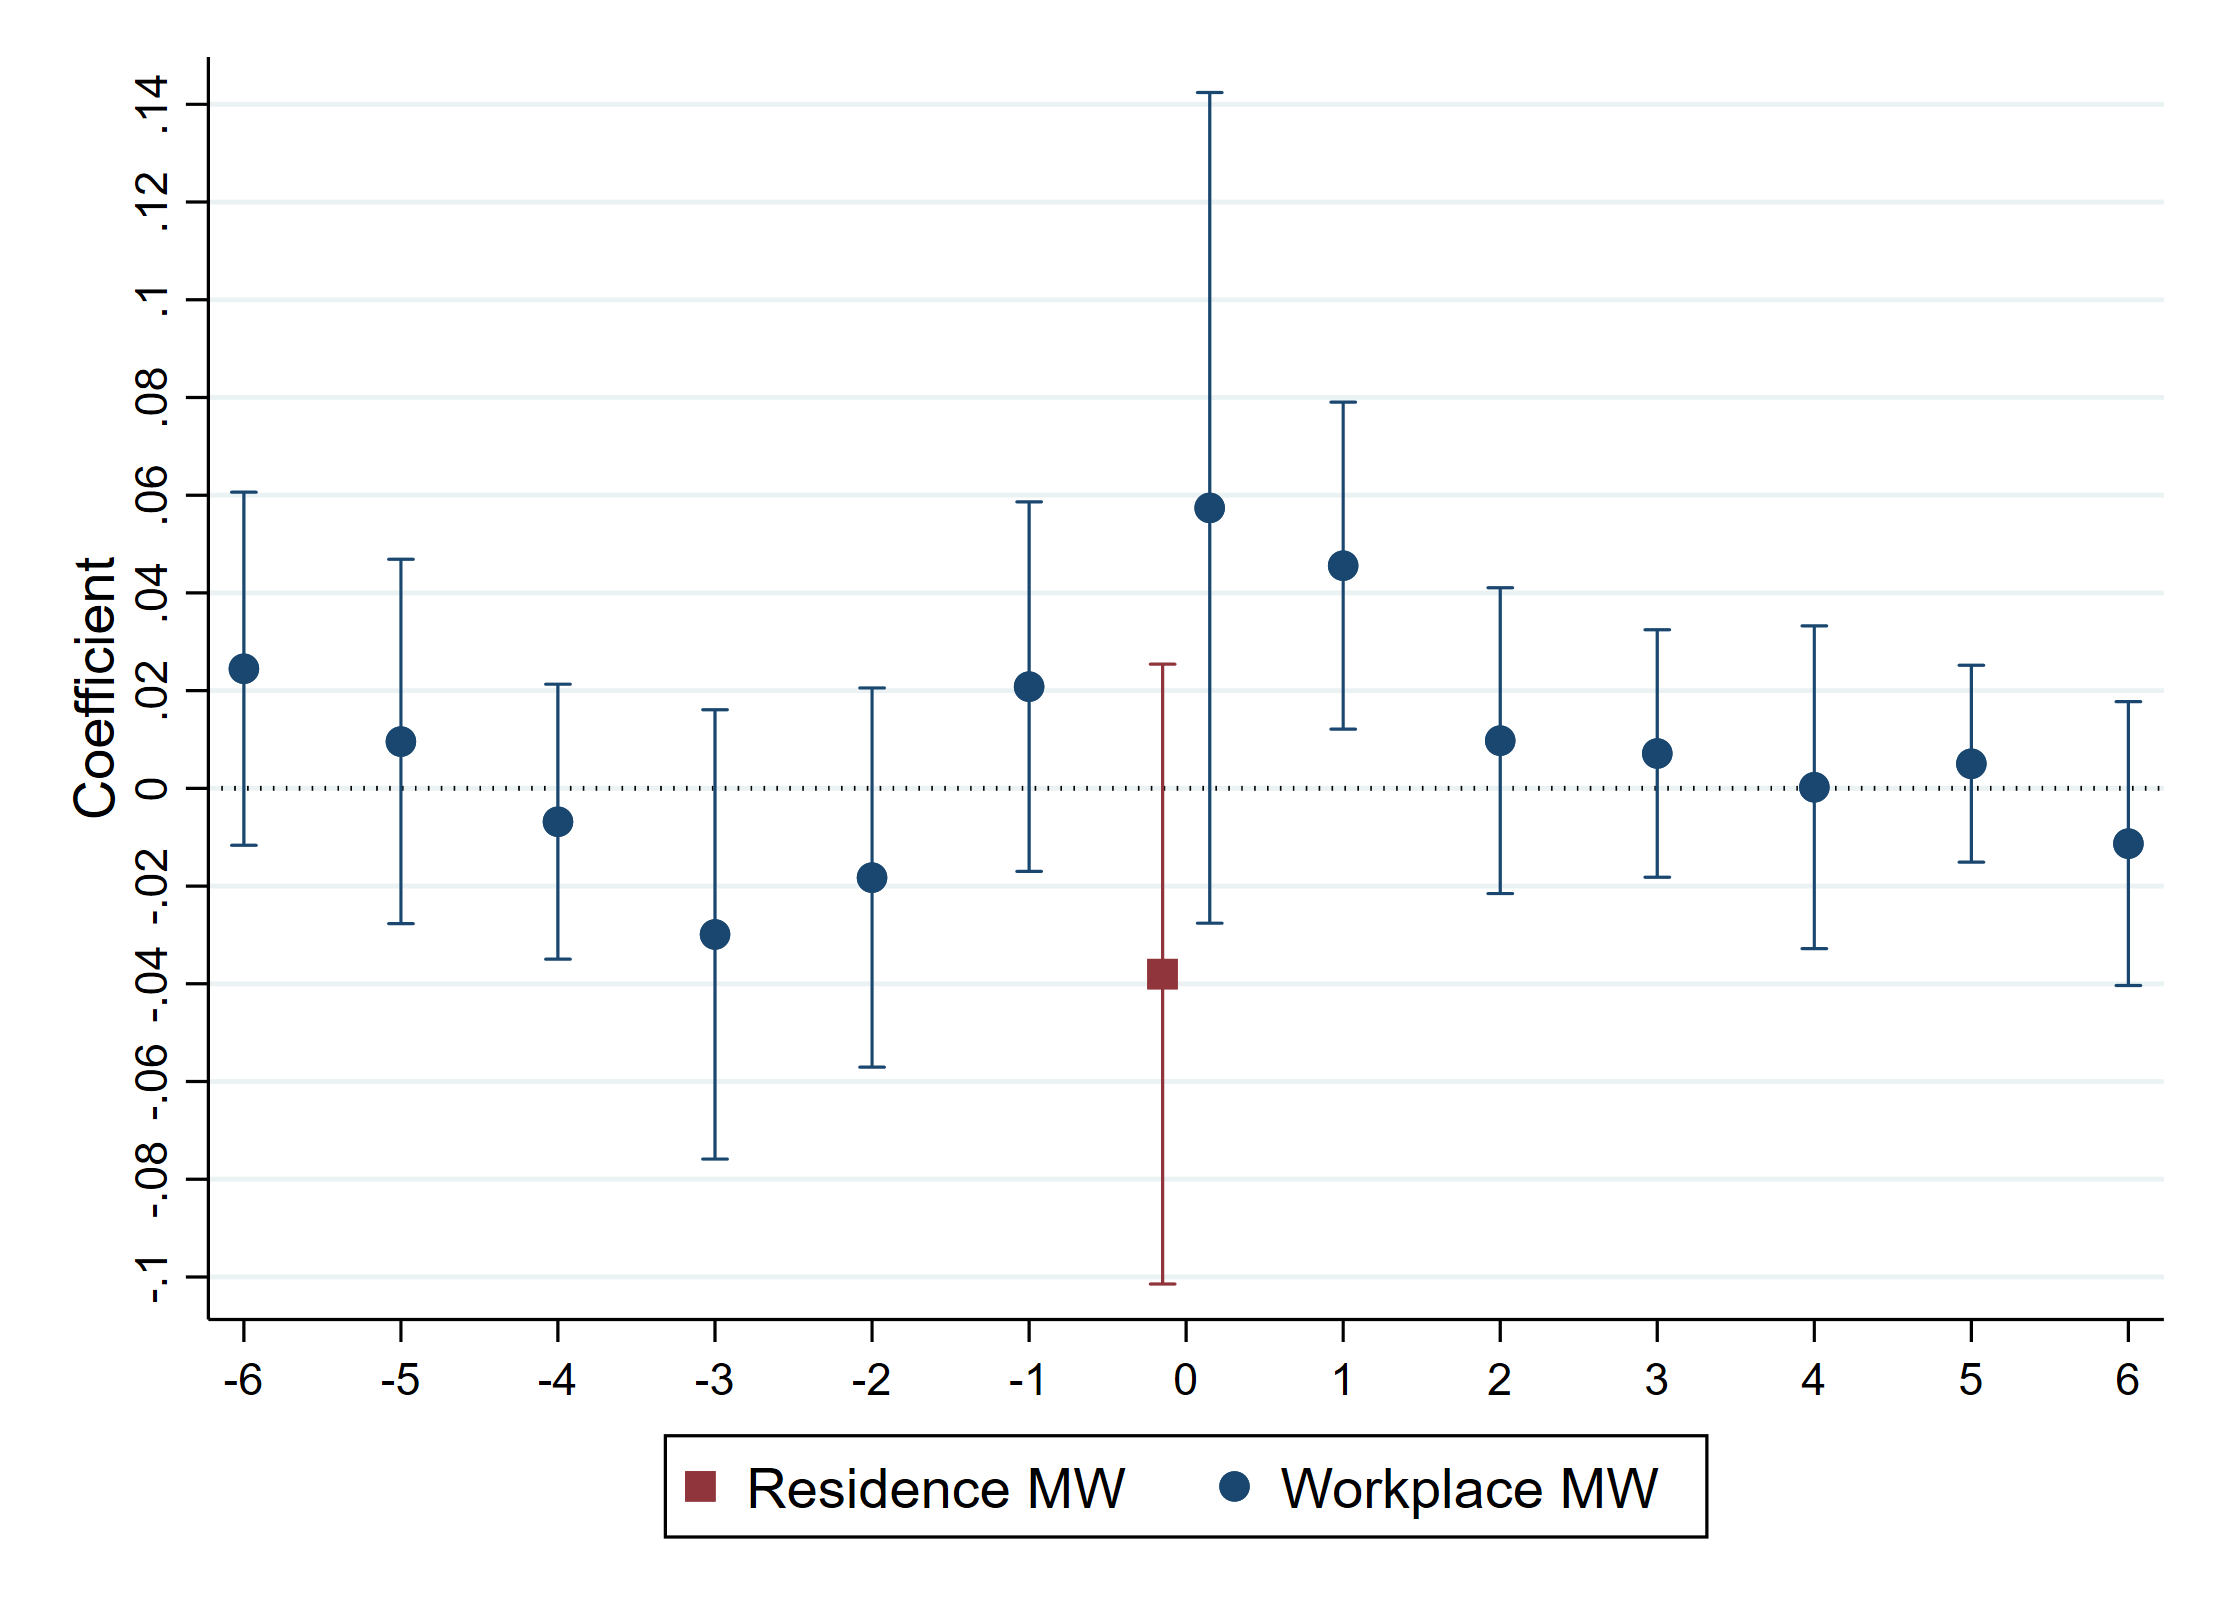
\includegraphics[width = 0.8\textwidth]{fd_geos_times/output/fd_both_mw_wkp_only_dynamic.png}

    \begin{minipage}{.95\textwidth} \footnotesize
        \vspace{3mm}
        Notes:
        Data are from the a county by month panel described in Section 
        \ref{sec:data_final_panel}.
        We plot coefficients from regressions of the log of rents per
        square foot on the residence and workplace MW measures, including 
        six leads and lags of the workplace MW measure.
        All regressions are estimated in first differences and include 
        time-period fixed effects and economic controls that vary at the 
        county and month levels.
        The measure of rents per square foot correspond to the Single Family, 
        Condominium and Cooperative houses from Zillow.
        The residence MW is defined as the log statutory MW at the County.
        The workplace MW is defined as the log statutory MW where the average 
        resident of the county works, constructed using LODES 
        origin-destination data.
        Economic controls from the QCEW include the change of the following 
        variables: the log of the average wage, the log of employment, and the 
        log of the establishment count for the sectors ``Information,'' 
        ``Financial activities,'' and ``Professional and business services.''
        95\% pointwise confidence intervals are obtained from standard errors 
        clustered at the state level.
    \end{minipage}
\end{figure}

\clearpage
\begin{figure}[h!]
    \centering
    \caption{Distribution of counterfactual increases in minimum wage measures,
             urban ZIP codes}
    \label{fig:cf_hist_res_and_wkp_mw}
    \begin{subfigure}{0.5\textwidth}
        \caption*{Residence MW}
        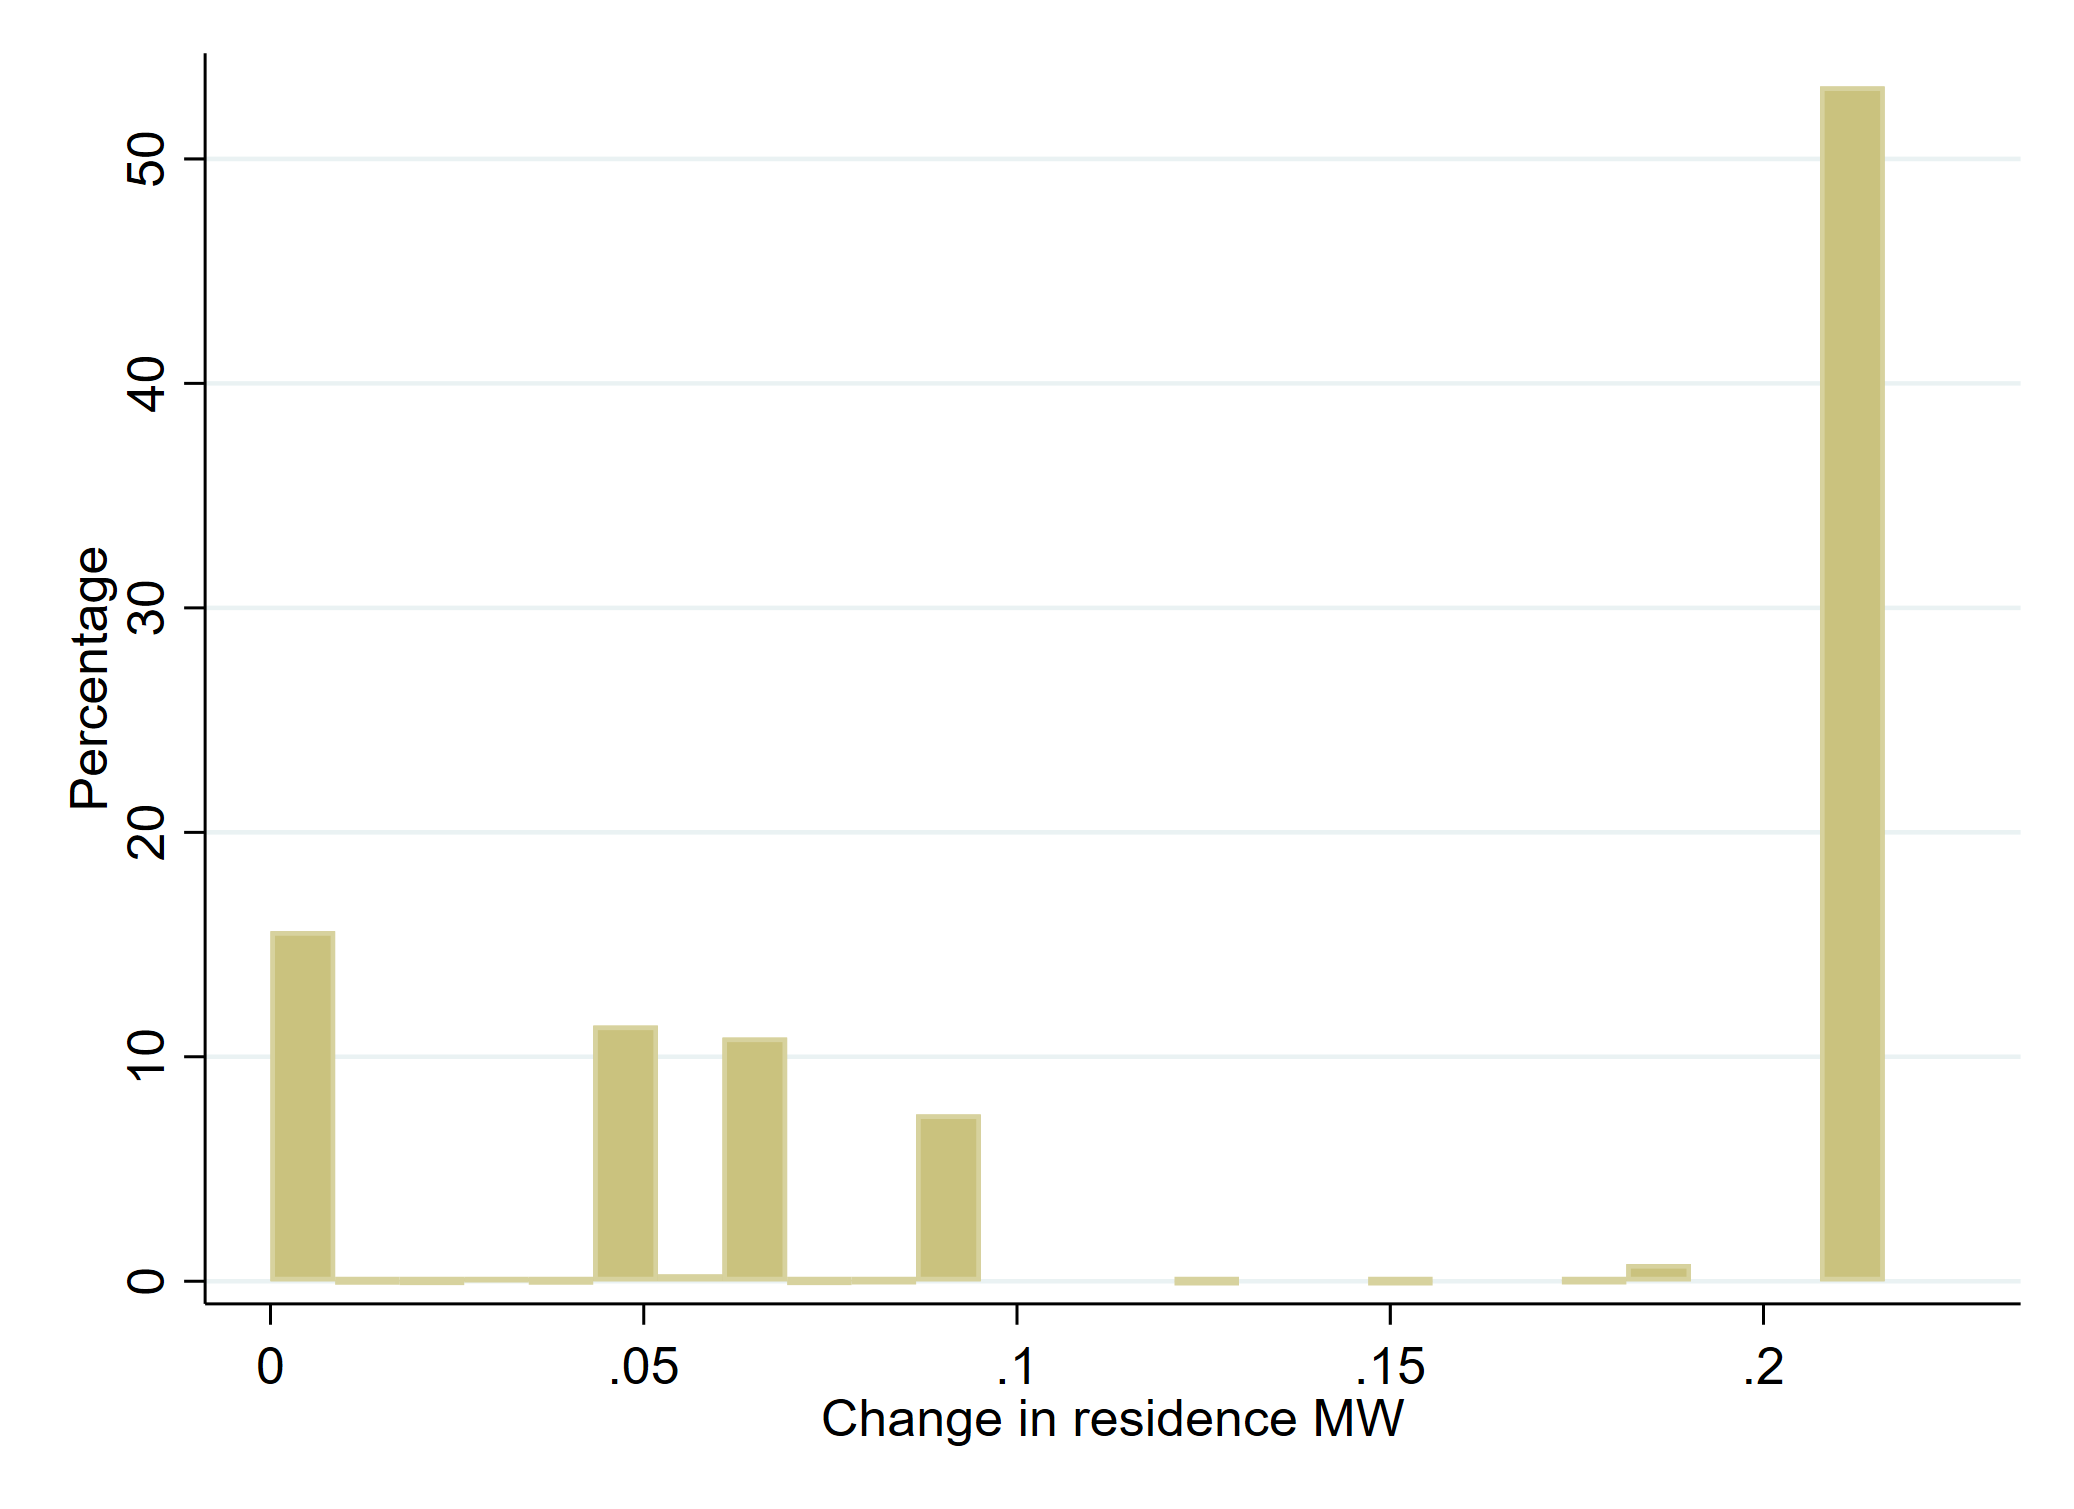
\includegraphics[width = 1\textwidth]{counterfactuals/output/hist_d_mw_res.png}
    \end{subfigure}%
    \begin{subfigure}{0.5\textwidth}
        \caption*{Workplace MW}
        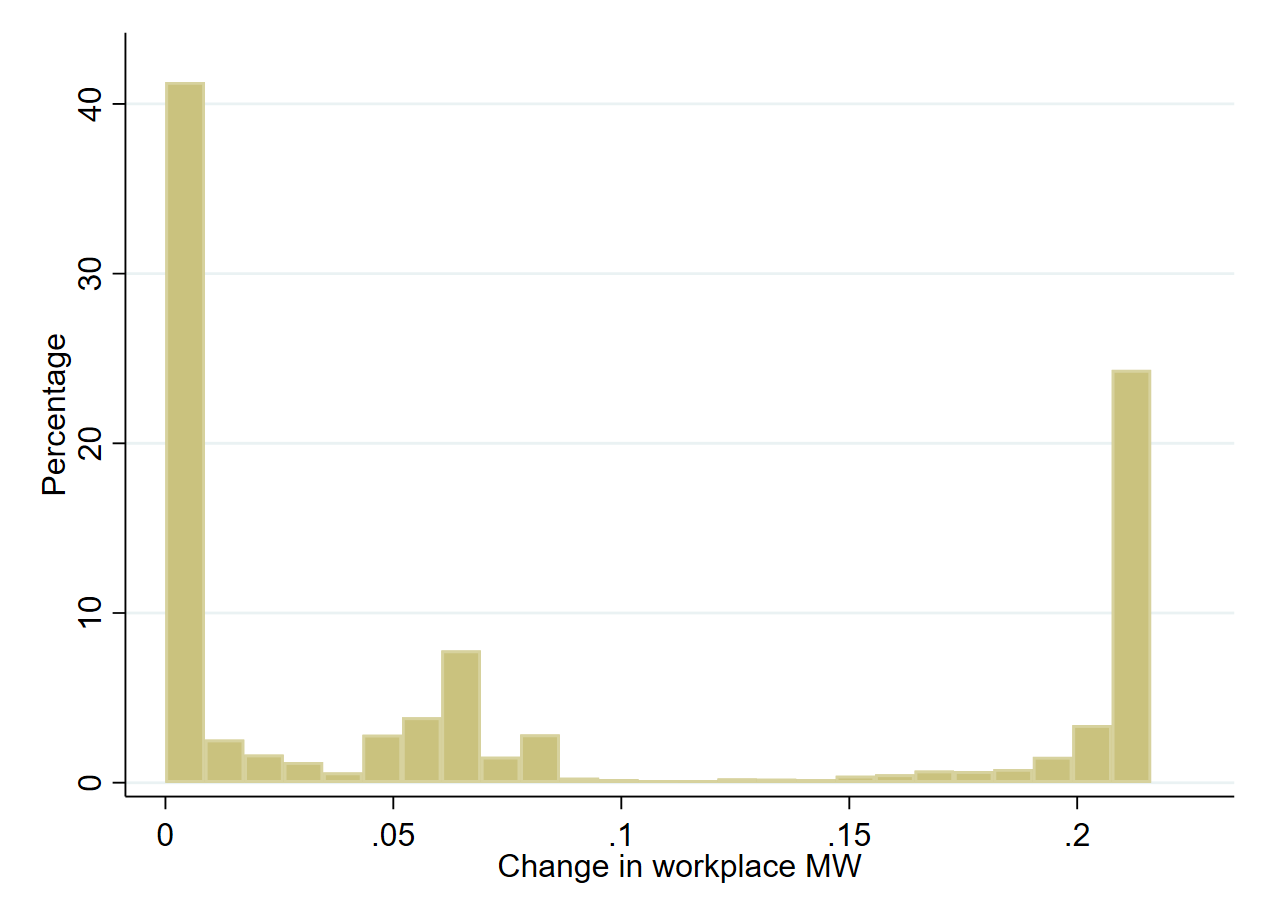
\includegraphics[width = 1\textwidth]{counterfactuals/output/hist_d_mw_wkp.png}
    \end{subfigure}

    \begin{minipage}{.95\textwidth} \footnotesize
        \vspace{3mm}
        Notes:
        Data are from LODES and the MW panel described in Section
        \ref{sec:data_mw_panel}.
        The figures show the distribution of changes in the residence and 
        workplace MW measures generated by a counterfactual increase to \$9 
        in the federal MW in January 2020, holding constant other MW policies 
        in their December 2019 levels.
        The unit of observation is the urban ZIP code, where we define a ZIP code 
        as urban if it belongs to a CBSA with at least 80\% of its population 
        classified as urban by the 2010 Census.
    \end{minipage}
\end{figure}



\end{document}
